\documentclass[11pt,a4paper]{article}
\usepackage[utf8]{inputenc}
\usepackage{cmap}
\usepackage[T1]{fontenc}
\usepackage[english]{babel}
\usepackage[margin=2cm]{geometry}
\usepackage[table]{xcolor}
\usepackage{enumitem}
\usepackage[hypertexnames=false]{hyperref}
\usepackage{tcolorbox}
\tcbuselibrary{breakable}
\usepackage{titlesec}
\usepackage{graphicx}
\usepackage{float}
\usepackage{booktabs}
\usepackage{tikz}
\usetikzlibrary{shapes.geometric, positioning, arrows, calc}
\usepackage{forest}
\usepackage{amsmath}
\usepackage{amssymb}
\usepackage{eurosym}
\usepackage[final]{microtype}
\microtypesetup{expansion=false}

% ===================================================================
% Color Palette: Tech Blue + Grey + Black + Orange Accent
% ===================================================================
\definecolor{primaryColor}{HTML}{0054A6}   % Tech blue
\definecolor{secondaryColor}{HTML}{374151}  % Dark grey
\definecolor{backgroundColor}{HTML}{F5F6FA} % Light grey
\definecolor{borderColor}{HTML}{D1D5DB}    % Medium grey
\definecolor{accentGreen}{HTML}{059669}    % Tech green
\definecolor{accentOrange}{HTML}{EA580C}   % Orange accent
\definecolor{accentRed}{HTML}{DC2626}      % Red
\definecolor{accentPurple}{HTML}{7C3AED}  % Purple — solweb.tper.it
\definecolor{accentViolet}{HTML}{8B5CF6}  % Violet — Punti Tper
\definecolor{accentTeal}{HTML}{0D9488}    % Teal — Tabaccherie
\definecolor{sectionBg}{HTML}{EBF0F7}      % Light blue bg

\hypersetup{
    colorlinks=true,
    linkcolor=primaryColor,
    urlcolor=primaryColor,
}

% ===================================================================
% Tcolorbox Styles (consistent palette, all breakable)
% ===================================================================
\tcbset{
    breakable,
    base/.style={
        colback=backgroundColor,
        colframe=borderColor,
        arc=2mm,
        left=6pt, right=6pt, top=6pt, bottom=6pt,
        boxsep=0pt,
    },
    sectionbox/.style={
        colback=primaryColor!8,
        colframe=primaryColor,
        arc=1mm,
        left=6pt, right=6pt, top=6pt, bottom=6pt,
        boxsep=0pt,
    },
    personabox/.style={
        colback=backgroundColor,
        colframe=primaryColor,
        arc=2mm,
        left=6pt, right=6pt, top=6pt, bottom=6pt,
        boxsep=0pt,
    },
    warningbox/.style={
        colback=accentOrange!5,
        colframe=accentOrange,
        arc=1mm,
        left=6pt, right=6pt, top=6pt, bottom=6pt,
        boxsep=0pt,
    },
    rffield/.style={
        colback=sectionBg,
        colframe=primaryColor,
        arc=1mm,
        left=6pt, right=6pt, top=6pt, bottom=6pt,
        boxsep=0pt,
    },
}

% ===================================================================
% Section Formatting (sans-serif headings, Tech Blue)
% ===================================================================
\titleformat{\section}
  {\color{primaryColor}\normalfont\Large\bfseries\sffamily}
  {}{0em}{}
  [\color{borderColor}\titlerule]

\titleformat{\subsection}
  {\color{secondaryColor}\normalfont\large\bfseries\sffamily}
  {}{0em}{}

\titleformat{\subsubsection}
  {\color{secondaryColor}\normalfont\normalsize\bfseries\sffamily}
  {}{0em}{}

% ===================================================================
% PGFPlots for charts
% ===================================================================
\usepackage{longtable}
\usepackage{pgfplots}
\pgfplotsset{compat=1.18}

% ===================================================================
% Screenshot / wireframe helper
% ===================================================================
\newcommand{\wfgraphic}[1]{%
  \includegraphics[width=\textwidth,keepaspectratio]{#1}%
}

% ===================================================================
% List spacing (compact)
% ===================================================================
\setlist{nosep, leftmargin=*}
\setlist[enumerate]{leftmargin=*, itemsep=2pt}
\setlist[itemize]{leftmargin=*, itemsep=2pt}

\begin{document}

\begin{tcolorbox}[colback=primaryColor,colframe=primaryColor,arc=1.5mm,halign=center,valign=center,height=2.5cm]
    \color{white}\LARGE\bfseries\sffamily UX DESIGN PROJECT: HELP PEOPLE HELP PEOPLE \\[0.2cm]
    \color{white!80}\small\sffamily TPER S.p.A. --- Design Proposal 2025/2026
\end{tcolorbox}

\vspace{0.3cm}

% ================================================================
% TEAM CARD — Valid for the entire project
% ================================================================
\section*{Team Card}

\vspace{0.2cm}

\begin{tcolorbox}[base]
\small
\textbf{Team Name}: UX Design Project --- Help People Help People \\[6pt]
This document constitutes the redesign project for the TPER S.p.A. digital ecosystem,
developed as part of the \textit{UUXD Design} course at the University of Bologna,
A.Y.\ 2025/2026. The Team Card is unique and valid for all project phases (Phase A, B, C, D).
\end{tcolorbox}

\vspace{0.3cm}

\begin{minipage}[t]{0.48\textwidth}
\begin{tcolorbox}[personabox]
    \textbf{Member 1} \\[4pt]
    \textbf{Name:} Francesco Castaldi \\[2pt]
    \textbf{Student ID:} 0001230662 \\[2pt]
    \textbf{Email:} francesco.castaldi4@studio.unibo.it \\[2pt]
    \textbf{Course:} Computer Science and Engineering (L-08)
\end{tcolorbox}
\end{minipage}
\hfill
\begin{minipage}[t]{0.48\textwidth}
\begin{tcolorbox}[personabox]
    \textbf{Member 2} \\[4pt]
    \textbf{Name:} Stefano Mercurio \\[2pt]
    \textbf{Student ID:} 1237578 \\[2pt]
    \textbf{Email:} stefano.mercurio@studio.unibo.it \\[2pt]
    \textbf{Course:} Computer Science and Engineering (L-08)
\end{tcolorbox}
\end{minipage}

\vspace{0.4cm}

\section{Client Card}

\subsection{Name of the Client}
\textbf{TPER S.p.A.} (Trasporto Passeggeri Emilia-Romagna).

\subsection{Description of the Client}
TPER is the main public transport company of Emilia-Romagna,
established in 2012 through the merger of ATC (Bologna and Ferrara) and FER
(Ferrovie Emilia Romagna). It operates on rubber --- urban, suburban, and
interurban mobility in the provinces of Bologna and Ferrara --- and on rail
with regional service. Headquartered in Bologna; main shareholders are
the Emilia-Romagna Region, the Municipality of Bologna, and the Metropolitan
City of Bologna.

\subsection{Name of the Tool}
\textbf{TPER Digital Ecosystem: Official Website}
(\url{https://www.tper.it}) and e-commerce platform
(\url{https://solweb.tper.it}).

\subsection{How to access the Tool?}
Access is via the web at two levels:
\begin{enumerate}[leftmargin=*]
    \item \textbf{Open:} consultation of timetables, alerts, and real-time
    journey planning, without registration.
    \item \textbf{Authenticated:} purchase and renewal of subscriptions,
    card management, document upload for concessions, Boost top-up, and
    penalty payment --- operations that currently require registration
    with personal credentials on the \texttt{solweb.tper.it} platform.
    Some services (title verification, zone calculation, tax code
    calculation) are already accessible without login.
\end{enumerate}

\subsection{Why should the Client want a new Tool?}
\begin{itemize}[leftmargin=*]
    \item The site is designed for users already experienced with public
    transport; vulnerable categories --- elderly, foreigners, people with low
    digital literacy --- struggle to navigate between the two platforms.
    \item Intermediaries (counter staff, social workers, volunteers,
    family members) lack tools to show, explain, and train in a
    structured way.
    \item At the counter, the public website is systematically bypassed
    in favour of proprietary terminals: the user remains a passive spectator
    and learns nothing. A platform designed for co-navigation would turn
    every contact into training.
\end{itemize}
Current impact: \textbf{queues} at counters, \textbf{digital autonomy}
blocked, increase in \textbf{procedural errors} and \textbf{refunds} handled
manually by TPER.

\subsection{Product Objectives for the Client}
\begin{itemize}[leftmargin=*]

    \item \textbf{Trainer-mode for structured assistance:}
    Provide counter staff and caregivers with integrated co-navigation
    tools --- checklists, visual highlighting, step-by-step guidance ---
    so that every contact with the vulnerable user becomes training and
    not delegation. For TPER: reduced pressure on counters and progressive
    migration of flows to the digital channel.

    \item \textbf{Autonomy on recurring operations:}
    High-frequency flows --- subscription renewal,
    timetable consultation, card top-up --- must become
    completable autonomously
    after a few guided sessions. For TPER: less dependence on the physical
    channel and call center, with direct savings on operating costs.

    \item \textbf{Removal of the registration barrier:}
    On the \texttt{solweb.tper.it} platform, operations such as the renewal
    of impersonal subscriptions, Boost top-up, and penalty payment
    (bus and rail) currently require creating an
    account. The redesign must introduce a guest path for these
    operations --- with only card number or tax code verification where
    necessary --- alongside the already free services
    (verifications, zone calculation). For TPER: capture users who today
    give up before even starting, increasing the transaction
    completion rate.

    \item \textbf{Multilingual support:}
    The main flows must be available in multiple languages to serve
    the growing share of foreign users. For TPER: fulfill the
    public service mission towards the entire user base,
    including the foreign component particularly present in
    Emilia-Romagna.

\end{itemize}

\subsection{Business Goals}
\begin{itemize}[leftmargin=*]
\item \textbf{Operational cost optimisation:} reduce front-office and
telephone support costs by migrating assisted flows to the web.
\item \textbf{Increased Customer Lifetime Value:} increase the subscription
renewal rate in advanced age groups, preventing abandonment of
public transport.
\item \textbf{Back-office process automation:} minimise human
intervention on complaints and data corrections, as an indirect effect
of a more autonomous user base and fewer procedural errors.
\end{itemize}

\subsection{Brand Identity}
The project strengthens TPER as a company close to citizens, capable of
combining digital innovation and social inclusion. No longer just a ticket
seller, but a guarantor of the right to mobility for all --- in line with
the institutional mission and the expectations of the shareholder entities.

\subsection{Success Metrics}
\begin{itemize}[leftmargin=*]
    \item \textbf{SUS Score (System Usability Scale):}
    perceived satisfaction, measured before and after the redesign.
    Target: $\geq 68/100$.

    \item \textbf{Task Completion Time:}
    average time to complete an assisted transactional flow.
    Target: $\leq 180$ seconds in trainer-mode.

    \item \textbf{Reduction in procedural errors:}
    wrong clicks, backtracking, and help requests per test session.
    Target: significant reduction compared to the current website.
\end{itemize}

\newpage
\section{User Segmentation card}

\subsection{Segmentation dimensions chosen}

\begin{tcolorbox}[base]
\begin{itemize}[leftmargin=*,itemsep=4pt]
    \item \textbf{Age group} --- indicator of the generational gap
    and familiarity with the local TPL.
    \item \textbf{Origin or nationality} --- proxy for language
    barriers and systemic familiarity.
    \item \textbf{Digital competence} --- level of autonomy
    in using web interfaces.
    \item \textbf{Training context} --- physical and
    relational environment in which coaching takes place.
    \item \textbf{TPL usage frequency} --- driving factor
    of learning motivation.
\end{itemize}
\end{tcolorbox}

\vspace{0.4cm}

\subsection{Reason for choice}

The five dimensions capture the three critical axes of the HPHP project:
\textbf{who} needs help (age, origin), \textbf{what} blocks them
(digital competence, language barrier), and \textbf{where} coaching
takes place (training context, usage frequency). For example:
an elderly Italian woman has known TPER routes for decades but gets stuck in the
transition from the informational site to the purchase platform; a young
foreigner is comfortable with a smartphone but cannot decipher bureaucratic
terms.

\vspace{0.4cm}

\begin{tcolorbox}[base]
\subsection{Segments within each dimension}
\begin{itemize}[leftmargin=*,itemsep=4pt]
\item \textbf{Age} --- 18--35 / 36--64 / 65+
\item \textbf{Origin} --- Italian / Foreign
\item \textbf{Digital competence} --- Low / Medium / High
\item \textbf{Training context} --- Domestic / Institutional /
Associational
\item \textbf{Usage frequency} --- Rare / Occasional / Frequent
\end{itemize}
\end{tcolorbox}

\vspace{0.2cm}
\begin{flushleft}
\textbf{Total combinations:}
\quad $2 \times 3 \times 3 \times 3 \times 3 = \mathbf{162}$
\end{flushleft}
\vspace{0.2cm}

\subsection{Chosen segmentation combinations}

\begin{tcolorbox}[base]
\begin{itemize}[leftmargin=*,itemsep=6pt]
    \item \phantomsection\label{seg:anziana}
    \textbf{[S1] The elderly commuter}\\
    Italian / 65+ / Low competence / Domestic / Frequent
    \item \phantomsection\label{seg:straniero}
    \textbf{[S2] The foreign worker}\\
    Foreign / 18--35 / Medium competence / Associational / Frequent
    \item \phantomsection\label{seg:cittadino}
    \textbf{[S3] The citizen at the counter}\\
    Italian / 36--64 / Low competence / Institutional / Occasional
\end{itemize}
\end{tcolorbox}

\vspace{0.4cm}

\subsection{Why these three combinations}

\begin{enumerate}[leftmargin=*]
    \item \textbf{The elderly commuter} is the core of the project:
    uses TPL every day but does not access digital services, delegating
    everything to a family member. The domestic context allows prolonged
    training sessions.
    \item \textbf{The foreign worker} reverses the problem:
    has medium digital competence but faces language and systemic
    barriers. The associational context enables patient,
    language-appropriate coaching.
    \item \textbf{The citizen at the counter} embodies the most
    stressful scenario: middle-aged, low digital competence, institutional
    context with limited time. If the system works for him,
    it works for everyone.
\end{enumerate}

\vspace{0.4cm}

\subsection{Expected impact on design}

\begin{itemize}[leftmargin=*,itemsep=6pt]

    \item \textbf{Adaptation to the temporal context:}
    each flow must be completable in a short session
    (fast-track for S3) but also decomposable into saveable
    micro-objectives (deferred learning for S1).

    \item \textbf{Cognitive, linguistic, and access barrier:}
    the design acts on three levels --- flow simplification
    (step-by-step paths), language disambiguation (glossary,
    icons), and registration-free access on \texttt{solweb.tper.it}
    for impersonal subscription renewal, Boost top-up, and penalties.

    \item \textbf{Scalability of guidance tools:}
    the trainer-mode offers modular tools --- from simple
    step-by-step highlighting for short sessions (S3) to the control
    panel with checklist and progress saving for structured
    sessions (S1/S2).

\end{itemize}
% ================================================================
% MARKET RESEARCH CARD
% ================================================================

\newpage 

\section{Market Research Card \#1}

\subsection*{Segment of choice}
\begin{tcolorbox}[base]
\textbf{The elderly commuter} --- Italian / 65+ / Digital competence
low / Domestic context / Frequent TPL usage
\end{tcolorbox}

\subsection*{Reason for choice}
\begin{tcolorbox}[base]
This is the core of the project: uses TPL every day but does not access
digital services, delegating everything to a family member. ISTAT data confirm
the scale of the phenomenon at the national level, while direct
interviews explore emotional barriers and coaching dynamics.
\end{tcolorbox}

\subsection*{User research method employed: \textit{Available statistics, One-on-one interviews}}
\begin{tcolorbox}[base]
\textbf{Sources (Available statistics):}
\begin{itemize}[leftmargin=*]
  \item ISTAT, \textit{Cittadini e ICT --- Anno 2025}, comunicato stampa.\\
  \href{https://www.istat.it/comunicato-stampa/cittadini-e-ict-anno-2025/}{Link al comunicato stampa ISTAT}
  \item ISTAT, \textit{Cittadini e ICT --- Anno 2024}, 28 aprile 2025.\\
  \href{https://www.istat.it/wp-content/uploads/2025/04/REPORT_CITTADINI-E-ICT_2024.pdf}{Link al PDF del report}
\end{itemize}

\vspace{0.3cm}
\textbf{Interviews:} 3 interviews with target users (average duration
15 minutes), focused on: current digital autonomy, relational
dynamics during help requests, emotional barriers, and
willingness to learn independently.
\end{tcolorbox}

\subsection*{Overall results of the analysis}
\begin{tcolorbox}[base]
\textbf{Quantitative data (ISTAT):} \textbf{72.5\% of 65--74 year-olds}
use the Internet, a share that drops to \textbf{35.7\% among the over-75s}.
At least basic digital skills stand at \textbf{27.4\%}
in the 65--74 age group. The gender gap is marked: among women
over 75, only 30.5\% use the Internet, compared to 43.0\% of
men of the same age.

\vspace{0.2cm}
\textbf{Qualitative data (Interviews):} a strong sense of
inadequacy emerges. The typical dynamic is \textbf{total delegation}: the
family member executes without explaining. The interviewees fear ``making
irreversible damage'' but some declare themselves willing to learn,
if guided calmly, step by step.
\end{tcolorbox}

\subsection*{Expected impact on design}
\begin{tcolorbox}[base]

\begin{itemize}[leftmargin=*,itemsep=6pt]

    \item \textbf{Restructure the relational dynamic:}
    the trainer-mode must provide the intermediary with instructions on
    \textit{how} to guide --- contextual suggestions that redefine
    their role from executor to facilitator, actively inhibiting the
    total delegation observed in the interviews.

    \item \textbf{Assume no basic digital competence:}
    the ISTAT data (27.4\% digital skills in the 65--74 age group)
    requires that every interface element be self-explanatory.
    Each action must communicate its reversibility to
    neutralise the fear of irreversible error.

\end{itemize}
\end{tcolorbox}

\newpage
\section{Market Research Card \#2}

\subsection*{Segment of choice}
\begin{tcolorbox}[base]
\textbf{The citizen struggling at the counter} --- Italian /
36--64 years / Low digital competence / Institutional context /
Occasional TPL usage
\end{tcolorbox}

\subsection*{Reason for choice}
\begin{tcolorbox}[base]
Represents the most critical contact point between vulnerable user and
the TPER system. Field observation makes it possible to detect both the
real behaviour of the user and the operational constraints of the
institutional context.
\end{tcolorbox}

\subsection*{User research method employed: \textit{Field observation}}
\begin{tcolorbox}[base]
\textbf{Location:} Sportello TPER Bologna --- via Guglielmo Marconi 4
\\[0.3cm]
The observation detected: type of requests, degree of user passivity,
discomfort behaviours, handling times, and
involvement of the \texttt{tper.it} site during the interaction.
\end{tcolorbox}

\subsection*{Overall results of the analysis}
\begin{tcolorbox}[base]
Requests focus on subscription renewals, document upload,
and route information. The dynamic is one of \textbf{total passivity}:
the user waits while the operator solves everything on the proprietary terminal
(3--5 minutes for simple operations, over 10 for documentary procedures).
The public website is systematically bypassed. Queue
pressure prevents training, and when necessary documents are missing,
the user must return multiple times.
\end{tcolorbox}

\subsection*{Expected impact on design}
\begin{tcolorbox}[base]

\begin{itemize}[leftmargin=*,itemsep=6pt]

    \item \textbf{Thematic paths and visual feedback:}
    predefined flows (e.g. ``Subscription renewal'') quickly
    selectable, with a progress indicator always visible to
    mitigate queue anxiety.

    \item \textbf{Passivity is structural, not emotional:}
    unlike the domestic context, here it is the system itself ---
    the queue, the operator-facing terminal, the compressed time ---
    that excludes the user. The design must make user involvement
    the fastest path, not the slowest one.

    \item \textbf{Preventive checklist:} visual list of documents
    needed before starting a procedure, to reduce empty
    returns to the counter.

\end{itemize}
\end{tcolorbox}

% ================================================================
% Market Research Card #3 (continues)
% ================================================================
\newpage
\section{Market Research Card \#3}

\subsection*{Segment of choice \& Reason for choice}
\begin{tcolorbox}[base]
\textbf{The foreign worker} --- Foreign / 18--35 years /
Medium digital competence / Associational context / Frequent TPL
usage

\vspace{0.2cm}
Introduces a double barrier --- linguistic and systemic --- that
no other combination presents. Is comfortable with a smartphone
but struggles with technical-bureaucratic language. ISTAT data quantify
the relevance of the phenomenon at the national level.
\end{tcolorbox}
\subsection*{User research method employed: \textit{Available statistics, One-on-one interviews}}
\begin{tcolorbox}[base]
\textbf{Sources:}
\begin{itemize}[leftmargin=*]
  \item ISTAT, \textit{Indicatori demografici --- Anno 2024},
  comunicato stampa, 31 marzo 2025.\\
  \href{https://www.istat.it/comunicato-stampa/indicatori-demografici-anno-2024/}{Link al comunicato ISTAT}

  \item ISTAT, \textit{Censimento e dinamica della popolazione --- Anno 2024}, dicembre 2024.\\
  \href{https://www.istat.it/wp-content/uploads/2025/12/Censimento-e-dinamica-della-popolazione-Anno-2024.pdf}{Link al PDF del censimento}
\end{itemize}

\vspace{0.2cm}
\textbf{Interviews:} 2 one-to-one interviews with foreign workers
in an associational context (average duration 20 minutes), focused on:
browsing experience of the TPER site, understanding of bureaucratic
lexicon, strategies for bypassing language barriers, and
availability of support in the associational context.
\end{tcolorbox}
\subsection*{Overall results of the analysis}
\begin{tcolorbox}[base]
\textbf{Quantitative data (ISTAT):} as of 1 January 2025,
\textbf{5,422,000 foreign citizens} reside in
Italy (9.2\% of the population),
with an average age of \textbf{37.0 years} (vs 47.8 for Italians), confirming
a young, working-age population. \textbf{58.3\%} reside
in the North, with a strong presence in Emilia-Romagna.

\vspace{0.2cm}
\textbf{Qualitative data (Interviews):} in the associational context,
the intermediary is not always available, unlike the domestic
context. Interviewees request printable modules with
step-by-step instructions that they can consult autonomously,
especially during registration and the first purchase. The
language barrier is exacerbated when translation is missing in the
critical phases of the transactional flow.
\end{tcolorbox}
\subsection*{Expected impact on design}
\begin{tcolorbox}[base]
On the language and lexicon level: \textbf{short sentences, infinitive
verbs, no technical-bureaucratic terms} without explanation.
On the visual level: \textbf{explicit and universal icons} always
accompanied by text labels. The purchase platform offers the
interface in English only after login, making it inaccessible
precisely when the foreign user needs it most: during
registration and first access. In the associational context, where the
trainer is not always present, \textbf{printable modules} become
essential: the user must be able to carry an autonomous
reference of the steps to follow. These choices, designed for the most
extreme case, improve the experience for all vulnerable users.
\end{tcolorbox}

% ================================================================
\newpage
{\raggedright\section{Assessment of Existing Resource Card --- TPER}\par}

\textbf{This is the client's tool}\\
\textit{(i.e. the one to redesign)}

\bigskip

\subsection*{Name of Tool}

\noindent TPER Digital Ecosystem: Official Website (\url{https://www.tper.it})
and e-commerce platform (\url{https://solweb.tper.it}).

\subsection*{Platforms for Tool (devices, operating systems, etc.)}

\noindent Both platforms are accessible via browser from any
device (desktop, laptop, smartphone, tablet) on all major
operating systems. Transactional functions on \texttt{solweb.tper.it}
require registration with personal credentials (alternatively,
SPID and CIE are available). Information services, journey
planning, and some tools (title verification, zone calculation) are
accessible without login.

{\raggedright\subsection*{Main Purpose of Tool, Main Operations Allowed, Perceived Level of Adequacy to Professional Standards}\par}

\noindent The ecosystem has a dual function. On the informational site
(\texttt{tper.it}): consultation of timetables and routes in real time,
journey planning, service alerts. On the transactional platform
(\texttt{solweb}\discretionary{-}{-}{.}\texttt{tper.it}): purchase and renewal of subscriptions
(standard and discounted, nominative and impersonal), top-up of the
\textit{Mi Muovo} card, Boost top-up, penalty payment (bus and rail),
upload of documents for fare concessions. Some services
(title verification, zone calculation, tax code calculation) are accessible
without registration.

\noindent The level of adequacy to professional standards is
\textit{partial}: information functions are decently implemented,
while transactional flows present structural criticalities in terms of
label clarity, error handling, and support for non-expert
users, particularly the over-70s with low digital competence.

\subsection*{Main Strengths of Tool, Reason for Choice}

\begin{itemize}
    \item Broad functional coverage: the digital ecosystem covers both
    informational services (timetables, routes, alerts) and
    transactional ones (subscriptions, top-ups, penalties), with a
    recognisable institutional access point.
    \item Presence of journey planning and real-time service consultation.
    \item Basic accessibility guaranteed: the site is consultable without registration for information functions.
    \item Widespread system presence: TPER is the reference operator for a large territorial basin in Emilia-Romagna.
    \item Brand identity already recognisable and consolidated among local users.
\end{itemize}

\subsection*{Main Weaknesses of Tool}

\begin{itemize}
    \item Complex information architecture: the
    \texttt{tper.it} menu mixes heterogeneous items without visual hierarchy,
    while the transition to \texttt{solweb.tper.it} for transactions
    is not clearly signalled, disorienting the user.
    \item Non-simplified technical terminology: labels such as
    ``Mi Muovo card'' and ``Boost'' are used without contextual
    explanation.
    \item Mandatory registration as a barrier: the transactional
    platform requires account creation for any
    operation, without offering a guest path for impersonal
    renewals, top-ups, or penalties.
    \item No caregiver coaching mode: the site does not support shared view, co-browsable session, or trainer functions.
    \item Absence of contextual guided support: no activatable tooltip, no step-by-step flow, no voice or tactile guide.
    \item Insufficient error handling: the site does not guide the user in recovering from common errors such as failed payment or expired subscription.
    \item No progress monitoring: the intermediary has no tools to track the user's acquired skills and plan incremental training.
\end{itemize}

\subsection*{First Impressions --- Initial Exploration}

\noindent The first exploration of the \texttt{tper.it} site produces
an impression of \textbf{unmanaged complexity}. The homepage simultaneously
presents corporate news, service alerts, route calculation
widgets, and links to transactional areas, without a clear visual
hierarchy that guides the user towards the primary task. An external
observer would take several seconds to understand where to renew a
subscription. The transition to the \texttt{solweb.tper.it} platform,
with the registration requirement, constitutes a visible barrier
from the very first approach to transactional functions.

\noindent\textbf{Problems identified during the exploratory phase (pre-formal analysis):}

\begin{itemize}
    \item No guided path for first access.
    \item No visible primary CTA on the homepage.
    \item The site does not clearly communicate the path to purchase.
    \item The site does not warn in advance that transactional
    operations require creating an account on
    \texttt{solweb.tper.it}.
    \item No contextual help function.
\end{itemize}

\subsection*{Direct Analysis: System vs.\ Guidelines}

\noindent\textit{Analysis conducted according to UserFocus guidelines. For each issue, the violated guideline and its location in the system is indicated.}\\[2pt]
\raggedright\url{http://www.userfocus.co.uk/resources/guidelines.html}\par

\bigskip

\noindent The reference guidelines adopted are:

\begin{tabular}{ll}
\toprule
\textbf{\#} & \textbf{Guideline} \\
\midrule
G1 & Home page --- clarity of site objectives \\
G2 & Task orientation --- support for completing user tasks \\
G3 & Navigation and IA --- clarity of navigation structure \\
G4 & Forms and data entry --- form usability \\
G5 & Trust and credibility --- trust in the system \\
G6 & Writing and content quality --- language quality \\
G7 & Page layout and visual design --- visual hierarchy \\
G8 & Search --- content findability \\
G9 & Help, feedback and error tolerance --- error handling and support \\
G10 & Accessibility --- cognitive and motor accessibility \\
\bottomrule
\end{tabular}

\bigskip

\noindent\textbf{Issue D1 --- Violation G1, G7}\phantomsection\label{iss:D1}\\
\textit{Location: homepage tper.it}\\

\noindent The homepage does not immediately communicate the primary purpose of the
site. Corporate news, route change alerts, and transactional widgets
occupy equivalent space, without hierarchy. The elderly user cannot
identify within a few seconds where to renew a subscription. The lack
of a visible primary CTA forces menu exploration, increasing
cognitive load from the very first phases of interaction.

\bigskip

\noindent\textbf{Issue D2 — Violation G3}\phantomsection\label{iss:D2}\\
\textit{Location: main menu tper.it, general navigation structure}\\

\noindent The information architecture mixes purely
informational items (timetables, alerts) and links to the purchase platform
(renewal, top-up) without signalling the difference. The menu exceeds 200
items with a depth of up to five levels. Labels use internal
corporate terminology that does not match the target user's vocabulary.
The path to reach a subscription renewal requires more
than three clicks and is not linear.

\bigskip

\noindent\textbf{Issue D3 — Violation G6, G10}\phantomsection\label{iss:D3}\\
\textit{Location: site — labels, buttons, system messages}\\

\noindent The technical language used on the site is never simplified or contextually explained. No area offers glossaries, tooltips, or explanatory micro-copy near technical terms. For an elderly user with low digital literacy, these words are devoid of operational meaning and produce cognitive block.

\bigskip

\noindent\textbf{Issue D4 — Violation G9}\phantomsection\label{iss:D4}\\
\textit{Location: solweb.tper.it --- purchase and renewal flow}\\

\noindent The system does not guide the user in recovering from the most common errors: failed payment, expired subscription not renewed. In these cases, the site does not show clear error messages with instructions on how to proceed, generating call centre calls, counter queues, and refund requests.

\bigskip

\noindent\textbf{Issue D5 — Violation G4}\phantomsection\label{iss:D5}\\
\textit{Location: solweb.tper.it platform --- registration
flow}\\

\noindent The transactional platform \texttt{solweb.tper.it} requires
account creation for purchase and
payment operations: subscription renewal,
Boost top-up, penalty payment. No guest path exists.
Registration, while offering several access methods (personal
credentials, SPID, CIE), is not accompanied by explanations of what data
is needed, how long it takes, or whether an alternative exists. For an elderly
user with low digital competence, the mere request to ``create an
account'' is enough to cause abandonment.

\subsection*{Reverse Analysis: Guidelines vs.\ System}

\noindent\textit{Systematic guideline-by-guideline analysis, searching the system for functions that violate each guideline. Problems already identified in the Direct Analysis are omitted; only newly emerged violations are reported.}

\bigskip

\noindent\textbf{Issue R1 — Guideline G5 (Trust and Credibility)}\phantomsection\label{iss:R1}\\
\textit{Location: solweb.tper.it — purchase and online payment area}\\

\noindent The site does not provide adequate trust signals on the purchase screens: absence of payment security icons, lack of intermediate confirmations during the flow, and no order summary before final payment. For an elderly user who already distrusts online payments, this absence of reassurances increases anxiety and the probability of flow abandonment.

\bigskip

\noindent\textbf{Issue R2 — Guideline G8 (Search)}\phantomsection\label{iss:R2}\\
\textit{Location: tper.it site — internal search function}\\

\noindent The internal search function is not prominent, does not suggest related queries or autocomplete. A search for \textit{``elderly subscription''} returns results devoid of useful metadata (no date, no meaningful excerpt) to guide the user in the choice. The elderly user who uses search as a shortcut does not obtain useful answers and is forced to manually navigate the site structure.

\bigskip

\noindent\textbf{Issue R3 — Guideline G10 (Accessibility)}\phantomsection\label{iss:R3}\\
\textit{Location: tper.it site — texts, contrast, clickable areas}\\

\noindent Some sections feature text of reduced size, insufficient text/background contrast for users with mild visual impairment, and clickable areas too small for smartphone use. The dark mode present on the site does not offer genuine accessibility control (adjustable contrast, text size, accessible fonts), directly penalising the elderly target.

\bigskip

\noindent\textbf{Issue R4 — Guideline G2 (Task Orientation)}\phantomsection\label{iss:R4}\\
\textit{Location: TPER ecosystem --- distinction between planning
and purchase}\\

\noindent The separation between the informational site (\texttt{tper.it}) and the
purchase platform (\texttt{solweb.tper.it}) is not clearly
signalled. The user can plan a route on \texttt{tper.it}
without understanding that to purchase or renew a subscription they
must register on a different platform, with separate interface and
credentials. The operational risk is concrete: the user could board
the vehicle convinced they have a valid ticket.

\bigskip

\noindent\textbf{Issue R5 — Guideline G9 (Help, Feedback, Error
Tolerance)}\phantomsection\label{iss:R5}\\
\textit{Location: TPER ecosystem — absence of contextual
support and trainer mode}\\

\noindent Neither of the two platforms offers guidance tools
integrated into flows: there are no tooltips, step-by-step guides,
contextual FAQs, or assistants that can be activated during task execution.
Even more critically, there is no trainer mode that
allows an intermediary to guide the vulnerable user in a
structured and repeatable way, which is precisely the main need
of the HPHP project.

\newpage

\section{Assessment of Existing Resource Card --- ATAC}

\textbf{This is the competitor’s tool}\\
\textit{(i.e. one of the external benchmarks used for comparison)}

\subsection*{Name of the Tool}

\noindent ATAC Roma website (\url{https://www.atac.roma.it}) and
e-commerce platform MyAtac (\url{https://ecommerce.atac.roma.it}).

\subsection*{Platforms for the Tool (devices, operating systems, etc.)}

\noindent The site is accessible via browser on desktop, laptop, tablet, and smartphone, on all major operating systems. It offers online services related to tickets, subscriptions, assistance, and travel information. Some functions require access to the MyAtac area, while others are public. The site thus represents the main institutional entry point to the ATAC digital ecosystem.

\subsection*{Main Purpose of the Tool, Operations Allowed, Adequacy to Professional Standards}

\noindent The site has both an informational and a transactional function. It allows purchase and renewal of subscriptions, management of some card operations, requesting or topping up discounted tickets, accessing customer support, and consulting real-time service information. It also explains where to buy physical tickets and how to use digital tickets, including smartphone ticket validation rules. The tool is adequate on a professional level for breadth of services, but only partially so in terms of clarity for vulnerable users. 

\subsection*{Main Strengths of the Tool, Reason for Choice}

\begin{itemize}
    \item Broad coverage of user needs: tickets, subscriptions,
    assistance and information are accessible from the institutional
    site, which serves as the entry point to the digital ecosystem.
    \item \textbf{Interactive purchase guide:} a 5-step guided path
    (frequency, zone, days, number of trips) that recommends the
    most suitable ticket, reducing choice overload. It is the most
    interesting pattern to replicate for TPER.
    \item Diversified sales channels: in addition to the site, the user can
    purchase through partner apps (Tap \& Go, sms\&go, B+), offering
    alternatives to those who cannot or do not want to use the web.
    \item Support for both standard and discounted tickets, with a very
    broad user base.
    \item Availability of the English version of the site, absent on
    the TPER informational site and available on the purchase platform
    only after login.
\end{itemize}

\subsection*{Main Weaknesses of the Tool}

\begin{itemize}
    \item The site is dense and very text-heavy, thus increasing the cognitive load for new users.
    \item The main services are distributed across multiple pages and areas, and this weakens task orientation.
    \item The terminology assumes a certain familiarity with subscriptions, validation, and digital procedures.
    \item The distinction between informational pages and transactional pages is not always immediate.
    \item Support is available, but not always integrated at the exact moment when the user needs help.
\end{itemize}

\subsection*{First Impressions --- Exploratory Analysis}

\noindent The first impression of the ATAC site is that of a mature but demanding system. It offers many useful services, but presents them through a significant amount of information and with several paths that the user must interpret. For an experienced traveller this may be acceptable, but for an elderly person with low digital confidence it can be excessive. The site appears authoritative and complete, but not specifically designed to reassure the insecure user at the moment of action.

\noindent\textbf{Problems identified during the exploratory phase:}

\begin{itemize}
    \item The main objective is not always immediately visible on the homepage.
    \item The user must already know where to go before starting the task.
    \item Ticketing, assistance, and informational content are not always well separated.
    \item Some procedures are only explained after entering the right section.
    \item The site informs, but does not always reduce hesitation.
\end{itemize}

\subsection*{Direct Analysis: System vs.\ Guidelines}

\noindent\textit{Analysis conducted according to UserFocus guidelines. For each problem, the violated guideline, its location in the system, and the severity classification are indicated.}\\[2pt]
\raggedright\url{http://www.userfocus.co.uk/resources/guidelines.html}\par

\bigskip

\noindent The reference guidelines adopted are:

\begin{tabular}{ll}
\toprule
\textbf{\#} & \textbf{Guideline} \\
\midrule
G1 & Homepage --- clarity of site objectives \\
G2 & Task orientation --- support for completing tasks \\
G3 & Navigation and information architecture --- clarity of structure \\
G4 & Forms and data entry --- form usability \\
G5 & Trust and credibility --- perceived reliability \\
G6 & Writing and content quality --- language quality \\
G7 & Layout and visual design --- visual hierarchy \\
G8 & Search --- content findability \\
G9 & Help, feedback, and error tolerance --- support and recovery \\
G10 & Accessibility --- cognitive and motor accessibility \\
\bottomrule
\end{tabular}

\bigskip

\noindent\textbf{Issue D1 --- Violation G1, G7}\phantomsection\label{atac:D1}\\
\textit{Location: ATAC site homepage}\\

\noindent The homepage does not make it immediately evident what the main path is for those who want to perform a concrete action, such as buying or renewing a travel ticket. Institutional information, service content, and transactional items coexist without a sufficiently clear hierarchy. This forces the user to explore and interpret the site even before starting the task. For an elderly or insecure user, this entry threshold is too high.

\bigskip

\noindent\textbf{Issue D2 — Violation G3}\phantomsection\label{atac:D2}\\
\textit{Location: general site structure and service sections}\\

\noindent The information architecture distributes content across different sections and separate domains --- the institutional site, the MyAtac purchasing platform, support on a third domain --- without this fragmentation being made evident to the user. The user must decide alone where to start, how to move from information to action, and which section is the right one for their problem. This structure is acceptable for expert users, but not for those who need a linear and repeatable path. Navigation reaches up to four levels of depth in corporate sections. The user must decide alone where to start and how to move from information to action. This structure is acceptable for expert users, but not for those who need a linear and repeatable path.

\bigskip

\noindent\textbf{Issue D3 — Violation G6, G10}\phantomsection\label{atac:D3}\\
\textit{Location: informational texts, instructions on tickets and online services}\\

\noindent The site language is correct but often assumes familiarity with concepts such as activation, validation, MyAtac, digital ticket, and discounted tickets. Explanations are present, but not always contextual enough for a user entering the system with low confidence. As a result, the site informs, but does not always guide. Cognitive accessibility thus remains only partial, especially for users over 70.

\bigskip

\noindent\textbf{Issue D4 — Violation G9}\phantomsection\label{atac:D4}\\
\textit{Location: help pages and exception handling}\\

\noindent The site provides support and guidance, but does not build a genuine recovery experience when something goes wrong. If the user encounters a problem during purchase or ticket management, they must interpret the available instructions on their own. For someone who is already insecure, this may be enough to interrupt the process. The error is not accompanied in a sufficiently reassuring way.

\bigskip

\noindent\textbf{Issue D5 — Violation G4}\phantomsection\label{atac:D5}\\
\textit{Location: areas requiring MyAtac access and related forms}\\

\noindent Some services require access to the MyAtac area or the use of forms and preliminary steps that increase the entry threshold. Registration and profile management are functional, but add a mental load that can block users with low confidence. The problem is not the presence of the account, but the fact that the site does not make the initial transition smooth enough. For the HPHP target, this is a significant criticality.

\subsection*{Reverse Analysis: Guidelines vs.\ System}

\noindent\textit{Systematic guideline-by-guideline analysis, searching the system for functions that violate it. Problems already identified in the direct analysis are omitted; only newly emerged violations are reported.}

\bigskip

\noindent\textbf{Issue R1 — Violation G5 (Trust and Credibility)}\phantomsection\label{atac:R1}\\
\textit{Location: ATAC site as a whole}\\

\noindent The site is credible from an institutional point of view, but the number of paths and service areas can weaken the new user’s operational trust. When it is not immediately clear which channel is the right one for a given task, the user may perceive uncertainty even in a reliable system. The problem does not concern the reputation of the service, but its usability legibility. Trust is strong on the brand, less strong on the task.

\bigskip

\noindent\textbf{Issue R2 — Violation G8 (Search)}\phantomsection\label{atac:R2}\\
\textit{Location: informational pages and service sections of the site}\\

\noindent The search function is present via an icon in the header but is not immediately visible as a primary tool. It does not offer suggestions or autocomplete, and its effectiveness depends on the user's ability to formulate queries with the correct domain terminology. For vulnerable users, search does not compensate for the complexity of the architecture and does not replace a more guided structure.

\bigskip

\noindent\textbf{Issue R3 — Violation G10}\phantomsection\label{atac:R3}\\
\textit{Location: service pages, instructions and account-based paths}\\

\noindent Accessibility is present on a functional level, but the system remains demanding on a mental level. The user must distinguish between different types of content, understand the meaning of technical terms, and remember where they are in the path. This reduces the suitability of the site for users with low digital confidence. The problem is therefore cognitive before being visual or motor.

\bigskip

\noindent\textbf{Issue R4 — Violation G2}\phantomsection\label{atac:R4}\\
\textit{Location: path between information, purchase and ticket management}\\

\noindent The site supports the task, but does not make it immediately readable as a sequence of actions. Consulting, purchasing, activating, and managing a ticket are connected operations, but the system expects the user to already understand their relationship. This is poorly suited to an audience that needs a simple and reassuring mental model. The platform facilitates the task only after the user has already overcome the hardest part: understanding the task.

\bigskip

\noindent\textbf{Issue R5 — Violation G9}\phantomsection\label{atac:R5}\\
\textit{Location: support distributed throughout the site}\\

\noindent The site offers help, but not a genuine guided experience at the moment of action. In case of doubt or error, the user often has to transform instructions into concrete behaviour on their own. For the HPHP target this is not enough, because the main problem is not the lack of information but the lack of confidence in the moment of using it. The absence of more guided support therefore represents the most serious criticality.

\newpage

% ================================================================

% ================================================================
% PRELIMINARY USER TESTING CARD — Client's tool
% ================================================================

\newpage

\section{Preliminary User Testing Card --- Client's Tool}
\textit{(This test relates to the client's tool, i.e., the one that needs to be redesigned)}

\vspace{0.2cm}

\subsection*{Name of tool}
\begin{tcolorbox}[base]
TPER official website --- \url{https://www.tper.it} and \url{https://solweb.tper.it}
\end{tcolorbox}

\vspace{0.2cm}

\begin{center}
  {\color{primaryColor}\large\bfseries Testing protocol}
  \vspace{0.1cm}
  \color{borderColor}\hrule
\end{center}

\vspace{0.2cm}

\subsection*{Testing session setup}
\begin{tcolorbox}[base]
Test sessions were conducted \textbf{in person},
at the subject's home. The device used was
the researcher's laptop, with \textbf{Windows 11}
operating system, \textbf{Google Chrome} browser updated
to the latest available version, 1920{\texttimes}1080 screen resolution.
The researcher was present in the room and did not interact
with the subject during task execution but limited himself to explaining the purpose of the site and the activity, consistently
with the \textit{bottom line data} methodology.
\end{tcolorbox}

\vspace{0.2cm}

\subsection*{Testing method}
\textbf{Discount usability testing} (2--5 people)

\vspace{0.2cm}

\subsection*{List of tasks to test}
\begin{tcolorbox}[base]
\begin{enumerate}[leftmargin=*,itemsep=4pt]
  \item \textbf{Timetable search and consultation:} The user must
  find stops and timetables for a specific line (Line 39: Circolare periferica sinistra)
  \item \textbf{Route planning:} The user must use the features offered by the application to calculate a route by setting origin (Piazza Maggiore) and destination (Giardini Margherita).
  \item \textbf{Purchase of a monthly subscription:} The user
  must navigate the existing information architecture to
  find access to the purchase page for an impersonal
  monthly subscription.
  \item \textbf{Identification of concessions and requirements:}
  The user must search for the requirements and necessary documents to obtain fare reductions for the purchase of an
  annual subscription in relation to their condition (ISEE, elderly, etc.)
  \item \textbf{Subscription renewal:} The user
  must locate the area dedicated to the renewal of their travel pass.
\end{enumerate}
\end{tcolorbox}

\vspace{0.2cm}

\subsection*{Testing methodology}
\textbf{Bottom line data} --- the subject
performs the tasks alone, without interaction with the researcher.
This mode was chosen to collect clean
quantitative data on completion, time, and errors,
uninfluenced by verbalisation or dialogue with
the facilitator.

\vspace{0.2cm}

\subsection*{Metrics of Tests}
\begin{itemize}[leftmargin=*,itemsep=3pt]
  \item \textbf{Success} --- percentage of tasks completed
successfully.
  \item \textbf{Time} --- time taken to complete
each task (in seconds).
  \item \textbf{Errors} --- how many errors and which ones were made.
  \item \textbf{Satisfaction} --- measured at the end of the session
via SUS scale (10 items). Expected baseline target
$< 68/100$ on the current tool.
\end{itemize}

\vspace{0.2cm}

\subsection*{Recruitment of subjects}
\begin{tcolorbox}[base]

\textbf{Laura Palumbo} --- 70 years, F.\\[0.3cm]
\textit{Digital competence:} Low --- uses the smartphone
exclusively for calls and WhatsApp messages; has never
purchased anything online or used digital public
administration services.\\[0.2cm]
\textit{Domain competence:} Medium --- uses the city bus
daily to get to the centre of Bologna, using
a subscription acquired thanks to the help of family members.\\[0.2cm]
\textit{Similarity to the segment:} High --- profile
fully matching \textit{The elderly commuter}
\hyperref[seg:anziana]{[S1]}\\[0.2cm]
\textit{Connection with the researcher:} Researcher's aunt.

\vspace{0.2cm}

\textbf{Sergio Mercurio} --- 67 years, M.\\[0.3cm]
\textit{Digital competence:} Medium --- regularly uses
smartphone, email, and banking applications; is familiar
with web browsing but does not habitually use public
administration portals or complex online
purchase services.\\[0.2cm]
\textit{Domain competence:} Low --- does not use
TPL frequently as he does not live in the city of Bologna; may need it rarely when visiting his son who studies away from home.\\[0.2cm]
\textit{Similarity to the segment:} Good --- profile
matching the 65+ age group with medium digital competence.\\[0.2cm]
\textit{Connection with the researcher:} Researcher's father
(Stefano Mercurio).

\vspace{0.2cm}

\textbf{Chris Harper} --- 34 years, M.\\[0.3cm]
\textit{Digital competence:} High --- uses smartphone,
email, maps, and online services in English daily; is used
to searching for information on his own but does not know
Italian digital authentication and ticketing systems well.\\[0.2cm]
\textit{Domain competence:} Low-medium --- spent about 2 months in Bologna for work reasons and uses TPL
regularly to travel between home, city centre, and station; has already
purchased single tickets but has never renewed a
subscription online.\\[0.2cm]
\textit{Similarity to the segment:} High --- profile
matching \textit{the foreign worker}\hyperref[seg:straniero]{[S2]}\\[0.2cm]
\textit{Connection with the researcher:} Personal acquaintance
of the researcher through professional network.

\vspace{0.2cm}

\textbf{Maria Borriello} --- 79 years, F.\\[0.3cm]
\textit{Digital competence:} Very low --- owns a
smartphone used exclusively for scrolling
social networks (Facebook, family photos); has never
made online purchases, accessed public
administration portals, or used transactional digital
services of any kind.\\[0.2cm]
\textit{Domain competence:} Low --- uses TPL
for long journeys related to leisure visits; depends entirely on family members for everything
concerning the digital management of the travel pass.\\[0.2cm]
\textit{Similarity to the segment:} Very high --- profile
representing the most extreme case of the
\textit{The elderly commuter}\hyperref[seg:anziana]{[S1]} segment: over 75, very low digital competence
(passive device use only), no
experience with active online interactions, total dependence
on an intermediary for digital TPL management.\\[0.2cm]
\textit{Connection with the researcher:} Family acquaintance
of the researcher through proximity network.

\end{tcolorbox}

\vspace{0.2cm}
\subsection*{Modality of recruitment of subjects}
\refstepcounter{subsection}\label{sec:recruitment-modality-client}
\begin{tcolorbox}[base]
Recruitment took place thanks to the family ties of Stefano Mercurio for the first two subjects, while Chris Harper was recruited as a colleague of the researcher on assignment at the Italian office, with a selection criterion based on matching the target segment profile. Maria Borriello was recruited through the family proximity network of Francesco Castaldi, as his grandmother, and represents the most critical target profile of the project: an elderly woman over 75 with digital competence limited solely to passive device use, without any experience of active interaction with online services.
\end{tcolorbox}
\vspace{0.2cm}

\subsection*{Motivation for choice of subjects}
\refstepcounter{subsection}\label{sec:recruitment-motivation-client}
\begin{tcolorbox}[base]
The subjects were chosen because they fully correspond
to the priority segmentation combination identified
in the project and were available and reachable for the
researchers. It is honest to acknowledge that the choice was
also determined by ease of access: two subjects
are family members of the researcher, one is a direct
acquaintance available for a credible simulation of a
foreign user, and Maria Borriello was involved
through the proximity network. Her inclusion responds
to a precise design need: expanding the sample
towards the over-75 profile with exclusively passive
digital use, the statistically most fragile group according
to 2025 ISTAT data and so far unrepresented by a distinct
subject in the test sample.
\end{tcolorbox}

% ================================================================
% TEST #1
% ================================================================

\newpage
\begin{center}
  {\color{primaryColor}\large\bfseries Test \#1: Sergio Mercurio}\\
  \vspace{0.1cm}
  \color{borderColor}\hrule
\end{center}

\vspace{0.5cm}

\subsection*{Name}
\begin{tcolorbox}[base]
Sergio Mercurio
\end{tcolorbox}

\subsection*{Date of test}
\begin{tcolorbox}[base]
8 May 2026
\end{tcolorbox}

\subsection*{Assistant of test (team member)}
\begin{tcolorbox}[base]
Stefano Mercurio
\end{tcolorbox}

\subsection*{Context of test}
\begin{tcolorbox}[base]
Test sessions were conducted at the subject's home, in a
quiet room with natural light without the presence of other outside people. Total duration: 45
minutes (5 task + SUS completion).
\end{tcolorbox}

\subsection*{Quantitative data of tests}
\begin{tcolorbox}[base]
Tests were considered failed when the user gave up.
Times were measured with a dedicated timer.
\begin{center}
\renewcommand{\arraystretch}{1.4}
\begin{tabular}{clcccc}
\toprule
\textbf{Task} & \textbf{Description} &
\textbf{Result} & \textbf{Time (s)} &
\textbf{Errors} & \textbf{Backtrack} \\
\midrule
T1 & Timetable search        & \textbf{F} & 354 & 4 & 3 \\
T2 & Route planning           & \textbf{S} & 76  & 0 & 0 \\
T3 & Subscription purchase    & \textbf{S} & 245 & 2 & 2 \\
T4 & Concessions \& requirements & \textbf{F} & 312 & 6 & 5 \\
T5 & Subscription renewal     & \textbf{S} & 209 & 3 & 3 \\
\midrule
\multicolumn{2}{l}{\textbf{Totals / Averages}} &
\textbf{3/5 (60\%)} & \textbf{239.2 s} &
\textbf{3} & \textbf{2.6} \\
\bottomrule
\end{tabular}
\end{center}

\vspace{0.3cm}
\small S = Success \quad F = Failure \quad
Errors = wrong clicks or wrong paths \quad
Backtrack = returns to the previous page
\end{tcolorbox}

\subsection*{SUS score}
\begin{tcolorbox}[base]
\textbf{SUS Score: 40/100}\\[0.2cm]
\small Score below the acceptability threshold
(50/100). Indicates serious perceived usability problems,
consistent with the difficulties observed during the session.
\end{tcolorbox}

\subsection*{Useful suggestions from subjects}
\begin{tcolorbox}[base]
At the end of the session, the subject spontaneously observed: \textit{``They should focus more on what people want'' [English translation of original Italian: ``Dovrebbero concentrarsi di pi\`u su cosa vuole la gente'']}, perceiving the current interface as excessively dispersive and overloaded with elements irrelevant to the citizen.
\end{tcolorbox}

\subsection*{Outcomes and reflections useful for design}
\begin{tcolorbox}[base]
The reduced volume of errors and backtrack recorded in some phases is not a symptom of system fluidity. The subject, struggling in the face of the amount of information before him, prefers to spend prolonged time in laborious visual exploration of each individual screen rather than clicking randomly. This block is directly caused by disorientation on the homepage \textbf{(\hyperref[iss:D1]{D1})} and by the promiscuous information architecture \textbf{(\hyperref[iss:D2]{D2})}.

Specifically regarding the first task (\textit{Timetable search and consultation}), despite having visually isolated the line of interest, he was unable to locate the command to access timetable tables, complaining of a total lack of intuitiveness of the graphic components.
The tendency not to distinguish an interactive button from a static text string experimentally confirms the severity of \textbf{\hyperref[iss:R3]{R3}} (Visual and cognitive accessibility).

\begin{itemize}[leftmargin=*]
    \item \textbf{Affordance and visual contrast (\hyperref[iss:R3]{R3}):} Standardize buttons with clear geometric shapes and visual elevation from the background. Introduce marked \textit{hover} and \textit{focus} micro-interactions to make the distinction from static text immediate and unambiguous.
    \item \textbf{De-cluttering and progressive disclosure (\hyperref[iss:D1]{D1}, \hyperref[iss:D2]{D2}):} Streamline the layout by eliminating secondary informational elements (news, general notices).
\end{itemize}
\end{tcolorbox}

% ================================================================
% TEST #2
% ================================================================

\newpage
\begin{center}
  {\color{primaryColor}\large\bfseries Test \#2: Laura Palumbo}\\
  \vspace{0.1cm}
  \color{borderColor}\hrule
\end{center}

\vspace{0.5cm}

\subsection*{Name}
\begin{tcolorbox}[base]
Laura Palumbo
\end{tcolorbox}

\subsection*{Date of test}
\begin{tcolorbox}[base]
12 May 2026
\end{tcolorbox}

\subsection*{Assistant of test (team member)}
\begin{tcolorbox}[base]
Stefano Mercurio
\end{tcolorbox}

\subsection*{Context of test}
\begin{tcolorbox}[base]
Test sessions were conducted at the subject's home, in a
familiar and quiet environment. Total duration: 41 minutes
(5 task + SUS completion).
\end{tcolorbox}

\subsection*{Quantitative data of tests}
\begin{tcolorbox}[base]
Tests were considered failed when the user gave up.
Times were measured with a dedicated timer.
\begin{center}
\renewcommand{\arraystretch}{1.4}
\begin{tabular}{clcccc}
\toprule
\textbf{Task} & \textbf{Description} &
\textbf{Result} & \textbf{Time (s)} &
\textbf{Errors} & \textbf{Backtrack} \\
\midrule
T1 & Timetable search         & \textbf{F} & 211 & 3 & 0 \\
T2 & Route planning           & \textbf{F} & 203 & 6 & 0 \\
T3 & Subscription purchase    & \textbf{F} & 180 & 7 & 5 \\
T4 & Concessions \& requirements & \textbf{F} & 195 & 7 & 4 \\
T5 & Subscription renewal     & \textbf{S} & 130 & 2 & 1 \\
\midrule
\multicolumn{2}{l}{\textbf{Totals / Averages}} &
\textbf{1/5 (20\%)} & \textbf{183.8 s} &
\textbf{5.0} & \textbf{2.0} \\
\bottomrule
\end{tabular}
\end{center}

\vspace{0.3cm}
\small S = Success \quad F = Failure \quad
Errors = wrong clicks or wrong paths \quad
Backtrack = returns to the previous page
\end{tcolorbox}

\subsection*{SUS score}
\begin{tcolorbox}[base]
\textbf{SUS Score: 37.5/100}\\[0.2cm]
\small Score below the minimum acceptability threshold
(50/100).
\end{tcolorbox}

\subsection*{Useful suggestions from subjects}
\begin{tcolorbox}[base]
At the end of the session the subject clearly expressed her disorientation due to the excessive visual density of the interface, commenting:
\textit{``The interface is too cluttered, there is too much confusion and it's not clear where to go and what to do. I struggled to find the concessions section --- it was a really dispersive path.'' [English translation of original Italian: ``L'interfaccia \`e troppo ingombrante, c'\`e troppa confusione e non si capisce bene dove bisogna andare e cosa fare. Ho fatto fatica a trovare la sezione delle agevolazioni --- \`e stato un percorso veramente dispersivo'']}.
\end{tcolorbox}

\subsection*{Outcomes and reflections useful for design}
\begin{tcolorbox}[base]
The quantitative data records a critical usability picture, with a completion rate of \textbf{20\%} (1 task passed out of 5) and a \textbf{SUS score of 37.5/100}. The error analysis reveals peaks of 7 occurrences in tasks T3 and T4 and frequent \textit{backtrack}.

\medskip
\begin{enumerate}[leftmargin=*]
    \item \textbf{Task Orientation (\hyperref[iss:R4]{R4}):} Clearly signal to the user the transition from the informational site to the purchase platform, which today occurs without any notice and without explaining why the interface changes.
    \item \textbf{Prevention and Error Tolerance (\hyperref[iss:D4]{D4}):} Compensate the inability to autonomously recover from errors by introducing a micro-guided accompaniment and contextual feedback messages managed by the intermediary layer.
    \item \textbf{Shortcuts for protection flows (\hyperref[iss:D2]{D2}):} Extract the concessions section from the deep nodes of the information architecture, positioning it as a priority access point in the initial dashboard through a step-by-step guided path (\textit{wizard}).
    The other points have already been discussed in the previous test.
\end{enumerate}
\end{tcolorbox}

% ================================================================
% TEST #3
% ================================================================

\newpage
\begin{center}
  {\color{primaryColor}\large\bfseries Test \#3: Chris Harper}\\
  \vspace{0.1cm}
  \color{borderColor}\hrule
\end{center}

\vspace{0.5cm}

\subsection*{Name}
\begin{tcolorbox}[base]
Chris Harper
\end{tcolorbox}

\subsection*{Date of test}
\begin{tcolorbox}[base]
5 May 2026
\end{tcolorbox}

\subsection*{Assistant of test (team member)}
\begin{tcolorbox}[base]
Francesco Castaldi
\end{tcolorbox}

\subsection*{Context of test}
\begin{tcolorbox}[base]
Session held at the researcher's office, in a quiet and informal environment. Chris Harper lived in Bologna for about two months for work-related support at the Italian company and uses TPL for daily travel to the centre, the station, and the workplace. He demonstrated familiarity with smartphones, maps, and email, but encountered difficulties in understanding some Italian labels, in distinguishing between the informational and transactional parts, and in the authentication process. Total duration: 47 minutes (5 task + SUS completion).
\end{tcolorbox}

\subsection*{Quantitative data of tests}
\begin{tcolorbox}[base]
\begin{center}
\renewcommand{\arraystretch}{1.4}
\begin{tabular}{clcccc}
\toprule
\textbf{Task} & \textbf{Description} &
\textbf{Result} & \textbf{Time (s)} &
\textbf{Errors} & \textbf{Backtrack} \\
\midrule
T1 & Timetable search          & \textbf{S} & 226 & 3 & 4 \\
T2 & Route planning            & \textbf{S} & 301 & 4 & 5 \\
T3 & Subscription purchase     & \textbf{F} & 498 & 8 & 10 \\
T4 & Concessions \& requirements & \textbf{F} & 344 & 5 & 7 \\
T5 & Subscription renewal      & \textbf{F} & 389 & 7 & 9 \\
\midrule
\multicolumn{2}{l}{\textbf{Totals / Averages}} &
\textbf{2/5 (40\%)} & \textbf{352 s} &
\textbf{5.4} & \textbf{7.0} \\
\bottomrule
\end{tabular}
\end{center}
\vspace{0.3cm}
\small S = Success \quad F = Failure \quad
Errors = wrong clicks or wrong paths \quad
Backtrack = returns to the previous page
\end{tcolorbox}

\subsection*{SUS score}
\begin{tcolorbox}[base]
\textbf{SUS Score: 45/100}\\[0.2cm]
\small Score below the acceptability threshold (50/100). The perception of the system proved weak, with difficulties mainly related to language, understanding the required steps, and the presence of access barriers that are not well explained to a non-Italian user.
\end{tcolorbox}

\subsection*{Useful suggestions from subjects}
\begin{tcolorbox}[base]
At the end of the session the subject commented: \textit{``I can find the timetable, but once I need to buy or renew something, the process becomes harder to follow and I would need clearer guidance in English.''}

Useful suggestion from the subject: a more explicit and simple guide in English for purchase, renewal, and validation could reduce dependence on external help.
\end{tcolorbox}
\subsection*{Outcomes and reflections useful for design}
\begin{tcolorbox}[base]
Chris Harper's data confirm that a foreign user with good digital literacy can handle basic informational functions, but encounters strong difficulties in transactional flows. The 40\% completion rate shows that the problems do not depend only on technical competence, but also on language, terminology, and absence of contextual support. This result directly confirms the severity of Issue \textbf{\hyperref[iss:D3]{D3}} and Issue \textbf{\hyperref[iss:D5]{D5}}, i.e.\ non-simplified language and mandatory registration, which block even users capable of navigating autonomously. The failure on Tasks 3, 4, and 5 suggests that the redesign must introduce a guest-friendly path, more accessible language, and step-by-step guidance for purchase, concessions, and renewal. The SUS of 45/100 confirms a low usability perception and also reinforces Issue \textbf{\hyperref[iss:R5]{R5}}, because the system does not offer sufficiently guided support at the moment of action.
\end{tcolorbox}
% ================================================================
% TEST #4
% ================================================================

\newpage
\begin{center}
  {\color{primaryColor}\large\bfseries Test \#4: Maria Borriello}\\
  \vspace{0.1cm}
  \color{borderColor}\hrule
\end{center}

\vspace{0.5cm}

\subsection*{Name}
\begin{tcolorbox}[base]
Maria Borriello
\end{tcolorbox}

\subsection*{Date of test}
\begin{tcolorbox}[base]
15 May 2026
\end{tcolorbox}

\subsection*{Assistant of test (team member)}
\begin{tcolorbox}[base]
Francesco Castaldi
\end{tcolorbox}

\subsection*{Context of test}
\begin{tcolorbox}[base]
Test sessions were conducted at the subject's home, in a
quiet domestic environment with only the
researcher present. Maria Borriello is 79 years old and uses the
smartphone exclusively for passive scrolling of
social networks (mainly family photos on
Facebook); she has never interacted with websites, institutional
portals, or online purchase services. She required
a brief initial orientation phase on the device
(researcher's laptop) before being able to start the tasks,
as she had never used a trackpad. Total
duration: 71 minutes (5 task + SUS completion assisted
in the reading of items).
\end{tcolorbox}

\subsection*{Quantitative data of tests}
\begin{tcolorbox}[base]
\begin{center}
\renewcommand{\arraystretch}{1.4}
\begin{tabular}{clcccc}
\toprule
\textbf{Task} & \textbf{Description} &
\textbf{Result} & \textbf{Time (s)} &
\textbf{Errors} & \textbf{Backtrack} \\
\midrule
T1 & Timetable search          & \textbf{F} & 698 & 14 & 17 \\
T2 & Route planning            & \textbf{F} & 724 & 16 & 19 \\
T3 & Subscription purchase     & \textbf{F} & 612 & 12 & 15 \\
T4 & Concessions \& requirements & \textbf{F} & 543 & 10 & 13 \\
T5 & Subscription renewal      & \textbf{F} & 681 & 13 & 16 \\
\midrule
\multicolumn{2}{l}{\textbf{Totals / Averages}} &
\textbf{0/5 (0\%)} & \textbf{652 s} &
\textbf{13.0} & \textbf{16.0} \\
\bottomrule
\end{tabular}
\end{center}
\vspace{0.3cm}
\small S = Success \quad F = Failure \quad
Errors = wrong clicks or wrong paths \quad
Backtrack = returns to the previous page
\end{tcolorbox}

\subsection*{SUS score}
\begin{tcolorbox}[base]
\textbf{SUS Score: 27.5/100}\\[0.2cm]
\small Score far below the acceptability
threshold (50/100) and below any minimum usability
threshold. It represents the lowest value
recorded in the entire test cycle and is consistent with the
0\% completion rate and with the subject's
profile: no experience of active browser navigation,
no familiarity with digital transactional
flows, total absence of a mental reference
model for interaction with a website.
\end{tcolorbox}

\subsection*{Useful suggestions from subjects}
\begin{tcolorbox}[base]
At the end of the session the subject commented:
\textit{``I don't understand anything, I don't even know where to start. When I have to do these things my daughter does them, I could never do it alone.'' [English translation of original Italian: ``Non ci capisco niente, non so neanche da dove cominciare. Quando devo fare queste cose le fa mia figlia, io non potrei mai farlo da sola.'']}
Useful suggestion from the subject: total dependence on an intermediary
is perceived as normal and inevitable. The system offers
no point of entry for a user in this condition:
no visual signal, no guide, no
understandable point of
entry. The subject also expressed
disorientation already on the homepage, unable to
distinguish between the sections of the site nor to identify
a clear initial action.
\end{tcolorbox}
\subsection*{Outcomes and reflections useful for design}
\begin{tcolorbox}[base]
Maria Borriello's data define the limiting case of the project: a completion rate of 0\%, an average time per task of 652 seconds, and a SUS of 27.5/100 make it evident that the TPER website, in its current form, is inaccessible for an over-75 user with very limited digital experience. The failures do not concern only transactional functions, but also affect the simplest informational functions, confirming the criticality of \textbf{Issue \hyperref[iss:D1]{D1}} and \textbf{Issue \hyperref[iss:D4]{D4}}, i.e.\ unclear homepage and absence of guidance in error recovery. The fact that the subject cannot complete any task also reinforces \textbf{Issue \hyperref[iss:D2]{D2}} and \textbf{Issue \hyperref[iss:D3]{D3}}, because the navigation structure and the language used by the site are neither comprehensible nor orienting. The comparison with Laura Palumbo shows that even a few years of age difference and minimal active smartphone use produce a significant performance gap; extreme old age and the total absence of active digital interaction therefore constitute an autonomous barrier. The overall SUS of the four TPER tests is confirmed well below the acceptability threshold, reinforcing the need for a redesign centred on clarity, constant guidance, and drastic reduction of cognitive load.
\end{tcolorbox}
\newpage
% ================================================================
% PRELIMINARY USER TESTING CARD --- Competitor's tool
% ================================================================

\newpage
\section{Preliminary User Testing Card --- Competitor's Tool}
\textit{(This test relates to the competitor's tool, i.e., used as external benchmark)}
\vspace{0.2cm}

\subsection*{Name of tool}
\begin{tcolorbox}[base]
Official ATAC Rome website --- \url{https://www.atac.roma.it} and \url{https://ecommerce.atac.roma.it}
\end{tcolorbox}

\vspace{0.2cm}

\begin{center}
  {\color{secondaryColor}\large\bfseries Testing protocol}
  \vspace{0.1cm}
  \color{borderColor}\hrule
\end{center}

\vspace{0.2cm}

\subsection*{Testing session setup}
\begin{tcolorbox}[base]
The testing sessions were conducted \textbf{in person},
at the subject's home, in the same session as the TPER site test,
to ensure comparability of conditions.
The device used was the researcher's laptop,
with \textbf{Windows 11} operating system,
\textbf{Google Chrome} browser updated to the latest available
version, 1920\texttimes1080 screen resolution. The researcher
was present in the room but did not interact with the
subject during task execution, limiting themselves to explaining the purpose of the site and the activity, consistently
with the \textit{bottom line data} methodology.
\end{tcolorbox}

\vspace{0.2cm}

\subsection*{Testing method}
\textbf{Discount usability testing}
(2--5 people)

\vspace{0.4cm}

\subsection*{List of tasks to test}
\begin{tcolorbox}[base]
\begin{enumerate}[leftmargin=*,itemsep=4pt]
  \item \textbf{Search and consultation of timetables:} The user
  must identify the route of a specific surface line (Metro-C Colosseo-Pantano) and analyze its timetables.
  \item \textbf{Trip planning:} The user
  must plan a journey using public transport by entering a departure point and
  an arrival point (Colosseo-Villa Borghese)
  \item \textbf{Fare search and ticket choice:}
  The user must identify the most suitable ordinary travel ticket
  for their needs (e.g., Card over 65),
  verifying its price and validity zones.
  \item \textbf{Identification of requirements and documents:}
  Continue from the previous point by identifying the requirements and documents
  to be submitted.
  \item \textbf{Recharging travel tickets:}
  The user must locate the section for recharging the Metrebus Card,
  starting the procedure up to the summary screen.
\end{enumerate}
\end{tcolorbox}

\vspace{0.4cm}

\subsection*{Testing methodology}
\textbf{Bottom line data} --- the
subject performs the tasks alone without interaction with
the researcher, under the same conditions as the TPER test,
to ensure full comparability of quantitative data.

\vspace{0.2cm}

\subsection*{Metrics of tests}
\begin{itemize}[leftmargin=*,itemsep=3pt]
  \item \textbf{Success} --- percentage of tasks completed
  successfully.
  \item \textbf{Time} --- time taken to
  complete each task (in seconds).
  \item \textbf{Errors} --- number of wrong clicks,
  backtrack and wrong paths per task.
  \item \textbf{Satisfaction} --- measured at the end of the session
  using the SUS scale (10 items).
\end{itemize}

\vspace{0.2cm}

\subsection*{Recruitment of subjects}
\begin{tcolorbox}[base]
The same subjects recruited for the TPER site test
were involved in the ATAC site test, to ensure
full comparability of results.
\end{tcolorbox}

\vspace{0.2cm}

\subsection*{Modality of recruitment of subjects}
\begin{tcolorbox}[base]
Same recruitment modality described in the TPER site test
(Section~\ref{sec:recruitment-modality-client}). The subjects were
re-contacted directly to arrange a second testing
session.
\end{tcolorbox}

\vspace{0.2cm}

\subsection*{Motivation for choice of subjects}
\begin{tcolorbox}[base]
Same motivation as the TPER site test
(Section~\ref{sec:recruitment-motivation-client}): the subjects
were chosen for their representativeness of segments
S1 (elderly commuter), S2 (foreign worker) and S3
(citizen at the counter).
\end{tcolorbox}

% ================================================================
% TEST ATAC #1 — Sergio Mercurio
% ================================================================

\newpage
\begin{center}
  {\color{secondaryColor}\large\bfseries
  Test ATAC \#1: Sergio Mercurio}\\
  \vspace{0.1cm}
  \color{borderColor}\hrule
\end{center}

\vspace{0.5cm}

\subsection*{Name}
\begin{tcolorbox}[base]
Sergio Mercurio
\end{tcolorbox}

\subsection*{Date of test}
\begin{tcolorbox}[base]
8 May 2026
\end{tcolorbox}

\subsection*{Assistant of test (team member)}
\begin{tcolorbox}[base]
Stefano Mercurio
\end{tcolorbox}

\subsection*{Context of test}
\begin{tcolorbox}[base]
Session held at the subject's home, on the same day as the
TPER test. Total duration: 35 minutes (5 task +
SUS completion).
\end{tcolorbox}

\subsection*{Quantitative data of tests}
\begin{tcolorbox}[base]
Tests were considered failed when the user gave up.
Times were measured with a dedicated timer.
\begin{center}
\renewcommand{\arraystretch}{1.4}
\begin{tabular}{clcccc}
\toprule
\textbf{Task} & \textbf{Description} &
\textbf{Outcome} & \textbf{Time (s)} &
\textbf{Errors} & \textbf{Backtrack} \\
\midrule
T1 & Timetable search             & \textbf{S} & 133 & 2 & 0 \\
T2 & Trip planning & \textbf{S} & 165 & 3 & 2 \\
T3 & Fare search           & \textbf{F} & 240 & 6 & 5 \\
T4 & Discounts and requirements  & \textbf{S} & 263 & 5 & 3 \\
T5 & Purchase and recharge       & \textbf{S} & 189 & 4 & 0 \\
\midrule
\multicolumn{2}{l}{\textbf{Totals / Averages}} &
\textbf{4/5 (80\%)} & \textbf{154s} &
\textbf{4} & \textbf{2} \\
\bottomrule
\end{tabular}
\end{center}
\vspace{0.3cm}
\small S = Success \quad F = Failure \quad
Errors = wrong clicks or wrong paths \quad
Backtrack = returns to the previous page
\end{tcolorbox}

\subsection*{SUS score}
\begin{tcolorbox}[base]
\textbf{SUS score: 60 /100}\\[0.2cm]
\small Score above the acceptability threshold
(50/100), but still below the good usability threshold.
\end{tcolorbox}

\subsection*{Useful suggestions from subjects}
\begin{tcolorbox}[base]
At the end of the session, the subject spontaneously commented: \textit{``Il sito ha troppe scelte, non so quale biglietto prendere. Almeno a Bologna so che c'\`e l'abbonamento e basta''} [English: ``The site has too many choices, I don't know which ticket to get. At least in Bologna I know there's just the subscription and that's it''].

This observation highlights a clear phenomenon of \textit{choice overload} generated by the ATAC interface, confirming the relevance of \textbf{Issue} \hyperref[atac:D3]{D3} for the competitor (complexity in cognitive accessibility of fares).

Furthermore, the subject expressed the need for a \textbf{conversational assistant based on Artificial Intelligence} capable of dynamically guiding them through the various steps. This insight represents a design opportunity of high strategic value, equally applicable to the TPER ecosystem.
\end{tcolorbox}

\subsection*{Outcomes and reflections useful for design}
\begin{tcolorbox}[base]
The completion rate rises to \textbf{80\% on ATAC compared to 60\% recorded on TPER}, despite the subject having no prior familiarity with the Roman transport network.

This performance increase can be attributed to the fact that, having completed the session on TPER a few minutes earlier, the user had partially internalized and built a mental model of the navigation logic of local public transport portals, reducing the initial friction in executing basic information tasks (T1 and T2).

However, once entering the ATAC ticket office, the extreme information density of the layout induced such visual overload that it hid the filtering mechanisms for tickets present on the page. The user did not notice the operational filters, experimentally confirming the severity of \textbf{ATAC Issues \hyperref[atac:D1]{D1} and \hyperref[atac:D2]{D2}} (heavy visual architecture and non-obvious usage sequences). For the TPER redesign, this finding underscores that it is not enough to organize content into logical categories, but it is necessary to implement a strong \textbf{reduction of visual complexity} and \textit{progressive disclosure} systems to avoid disorienting the fragile target.
\end{tcolorbox}

% ================================================================
% TEST ATAC #2 — Laura Palumbo
% ================================================================

\newpage
\begin{center}
  {\color{secondaryColor}\large\bfseries
  Test ATAC \#2: Laura Palumbo}\\
  \vspace{0.1cm}
  \color{borderColor}\hrule
\end{center}

\vspace{0.5cm}

\subsection*{Name}
\begin{tcolorbox}[base]
Laura Palumbo
\end{tcolorbox}

\subsection*{Date of test}
\begin{tcolorbox}[base]
12 May 2026
\end{tcolorbox}

\subsection*{Assistant of test (team member)}
\begin{tcolorbox}[base]
Stefano Mercurio
\end{tcolorbox}

\subsection*{Context of test}
\begin{tcolorbox}[base]
Session held at the subject's home, on the same day as the TPER test. Total duration: 34 minutes (5 task +
SUS completion).
\end{tcolorbox}

\subsection*{Quantitative data of tests}
\begin{tcolorbox}[base]
\begin{center}
\renewcommand{\arraystretch}{1.4}
\begin{tabular}{clcccc}
\toprule
\textbf{Task} & \textbf{Description} &
\textbf{Outcome} & \textbf{Time (s)} &
\textbf{Errors} & \textbf{Backtrack} \\
\midrule
T1 & Timetable search             & \textbf{S} & 134 & 3 & 2 \\
T2 & Trip planning & \textbf{F} & 146 & 5 & 0 \\
T3 & Fare search           & \textbf{F} & 210 & 4 & 3 \\
T4 & Discounts and requirements  & \textbf{F} & 155 & 4 & 2 \\
T5 & Purchase and recharge       & \textbf{S} & 90 & 2 & 1 \\
\midrule
\multicolumn{2}{l}{\textbf{Totals / Averages}} &
\textbf{2/5 (40\%)} & \textbf{260 s} &
\textbf{3,6} & \textbf{1,6} \\
\bottomrule
\end{tabular}
\end{center}
\vspace{0.3cm}
\small S = Success \quad F = Failure \quad
Errors = wrong clicks or wrong paths \quad
Backtrack = returns to the previous page
\end{tcolorbox}

\subsection*{SUS score}
\begin{tcolorbox}[base]
\textbf{SUS score: 30/100}\\[0.2cm]
\small Score below the minimum usability
threshold (50/100).
\end{tcolorbox}

\subsection*{Useful suggestions from subjects}
\begin{tcolorbox}[base]
At the end of the session the subject expressed strong frustration at the poor cognitive responsiveness of the interface, observing:
\textit{``La guida all'acquisto \`e utile, su TPER non c'\`e niente di simile. Inoltre la ricerca del percorso \`e snervante: inserisci l'indirizzo e invece di darti la soluzione migliore ti propone mille alternative ambigue, con una mappa microscopica in cui non si riesce a zoomare per orientarsi''} [English: ``The purchase guide is useful, on TPER there is nothing like it. Also, the route search is exasperating: you enter the address and instead of giving you the best solution it offers you a thousand ambiguous alternatives, with a microscopic map where you cannot zoom to orient yourself''].

\end{tcolorbox}

\subsection*{Outcomes and reflections useful for design}
\begin{tcolorbox}[base]
\noindent The suggestions and complaints define two lines of action:
\begin{itemize}[leftmargin=*]
    \item \textbf{Purchase Guide model:} ATAC's fare orientation function is an excellent operational support pattern to be reworked and integrated into the TPER redesign.
    \item \textbf{Linear planning interfaces (\hyperref[atac:D2]{D2}):} Avoid information overload in route calculation widgets. The fragile user does not want to explore systemic alternatives, but demands a single clear recommendation and a highly readable map.
\end{itemize}
\end{tcolorbox}

% ================================================================
% TEST ATAC #3 — Chris Harper
% ================================================================

\newpage
\begin{center}
  {\color{secondaryColor}\large\bfseries
  Test ATAC \#3: Chris Harper}\\
  \vspace{0.1cm}
  \color{borderColor}\hrule
\end{center}

\vspace{0.5cm}

\subsection*{Name}
\begin{tcolorbox}[base]
Chris Harper
\end{tcolorbox}

\subsection*{Date of test}
\begin{tcolorbox}[base]
5 May 2026
\end{tcolorbox}

\subsection*{Assistant of test (team member)}
\begin{tcolorbox}[base]
Francesco Castaldi
\end{tcolorbox}

\subsection*{Context of test}
\begin{tcolorbox}[base]
Session held at the researcher's office, on the same day as the TPER test. Total duration: 45 minutes (5 task + SUS completion).
\end{tcolorbox}

\subsection*{Quantitative data of tests}
\begin{tcolorbox}[base]
\begin{center}
\renewcommand{\arraystretch}{1.4}
\begin{tabular}{clcccc}
\toprule
\textbf{Task} & \textbf{Description} &
\textbf{Outcome} & \textbf{Time (s)} &
\textbf{Errors} & \textbf{Backtrack} \\
\midrule
T1 & Timetable search             & \textbf{S} & 192 & 2 & 3 \\
T2 & Trip planning & \textbf{S} & 268 & 3 & 4 \\
T3 & Fare search           & \textbf{S} & 341 & 4 & 5 \\
T4 & Discounts and requirements  & \textbf{F} & 377 & 5 & 7 \\
T5 & Purchase and recharge       & \textbf{F} & 406 & 7 & 9 \\
\midrule
\multicolumn{2}{l}{\textbf{Totals / Averages}} &
\textbf{3/5 (60\%)} & \textbf{317 s} &
\textbf{4,2} & \textbf{5,6} \\
\bottomrule
\end{tabular}
\end{center}
\vspace{0.3cm}
\small S = Success \quad F = Failure \quad Errors = wrong clicks or wrong paths \quad Backtrack = returns to the previous page
\end{tcolorbox}

\subsection*{SUS score}
\begin{tcolorbox}[base]
\textbf{SUS score: 51/100}\\[0.2cm]
\small Score just above the minimum acceptability threshold, but still far from the good usability threshold.
\end{tcolorbox}

\subsection*{Useful suggestions from subjects}
\begin{tcolorbox}[base]
At the end of the session the subject commented:
\textit{``I can find the timetable and ticket prices, but for discounts and online purchase I would need a clearer English path.''}
A more explicit and simple guide in English for purchase, renewal and discounts could reduce dependence on external support.
\end{tcolorbox}
\subsection*{Outcomes and reflections useful for design}
\begin{tcolorbox}[base]
Chris Harper's data shows that a foreign user with good digital literacy can manage basic information functions and fare consultation, but encounters difficulties in the more complex flows related to discounts and online purchase. The 60\% completion rate is higher than that recorded on TPER for the same subject, but remains insufficient for satisfactory autonomous use. The failure on Tasks 4 and 5 confirms the criticality of \textbf{Issue \hyperref[atac:D3]{D3}} and \textbf{Issue \hyperref[atac:D5]{D5}}, i.e., inaccessible language and overly burdensome authentication for those who do not know the local system well. The TPER redesign must therefore offer a guest-friendly path, clearer language and a step-by-step guide for purchase, discounts and renewal. The SUS of 51/100 confirms a perception of usability that is only minimally acceptable, highlighting that for non-Italian users the clarity of the steps is as crucial as the quality of the information.
\end{tcolorbox}

% ================================================================
% TEST ATAC #4 — Maria Borriello
% ================================================================

\newpage
\begin{center}
  {\color{secondaryColor}\large\bfseries
  Test ATAC \#4: Maria Borriello}\\
  \vspace{0.1cm}
  \color{borderColor}\hrule
\end{center}

\vspace{0.5cm}

\subsection*{Name}
\begin{tcolorbox}[base]
Maria Borriello
\end{tcolorbox}

\subsection*{Date of test}
\begin{tcolorbox}[base]
15 May 2026
\end{tcolorbox}

\subsection*{Assistant of test (team member)}
\begin{tcolorbox}[base]
Francesco Castaldi
\end{tcolorbox}

\subsection*{Context of test}
\begin{tcolorbox}[base]
Session held at the subject's home, on the same day as the TPER test. Total duration: 66 minutes (5 task + SUS completion).
\end{tcolorbox}

\subsection*{Quantitative data of tests}
\begin{tcolorbox}[base]
\begin{center}
\renewcommand{\arraystretch}{1.4}
\begin{tabular}{clcccc}
\toprule
\textbf{Task} & \textbf{Description} &
\textbf{Outcome} & \textbf{Time (s)} &
\textbf{Errors} & \textbf{Backtrack} \\
\midrule
T1 & Timetable search             & \textbf{F} & 511 & 11 & 14 \\
T2 & Trip planning & \textbf{F} & 546 & 12 & 15 \\
T3 & Fare search           & \textbf{F} & 478 & 10 & 13 \\
T4 & Discounts and requirements  & \textbf{F} & 603 & 13 & 16 \\
T5 & Purchase and recharge       & \textbf{F} & 624 & 14 & 17 \\
\midrule
\multicolumn{2}{l}{\textbf{Totals / Averages}} &
\textbf{0/5 (0\%)} & \textbf{552 s} &
\textbf{12,0} & \textbf{15,0} \\
\bottomrule
\end{tabular}
\end{center}
\vspace{0.3cm}
\small S = Success \quad F = Failure \quad Errors = wrong clicks or wrong paths \quad Backtrack = returns to the previous page
\end{tcolorbox}

\subsection*{SUS score}
\begin{tcolorbox}[base]
\textbf{SUS score: 29/100}\\[0.2cm]
\small Score well below the acceptability threshold (50/100) and consistent with the profile of a user who uses the smartphone only passively, without any active browsing experience.
\end{tcolorbox}

\subsection*{Useful suggestions from subjects}
\begin{tcolorbox}[base]
At the end of the session the subject commented:
\textit{``Non so proprio dove cliccare, per me queste cose le deve fare mia figlia o mio nipote''} [English: ``I really don't know where to click, for me these things have to be done by my daughter or grandson''].
Even on ATAC, a very elderly and digitally fragile user cannot orient themselves without explicit support, confirming the need for much more guided interfaces and simplified paths.
\end{tcolorbox}

\subsection*{Outcomes and reflections useful for design}
\begin{tcolorbox}[base]
Maria Borriello's data represents the limit case also on the ATAC competitor. The 0\% completion rate and SUS of 29/100 indicate that, despite some more accessible elements compared to TPER, the ATAC site remains inadequate for a user over 75 with very low digital competence. The total failure on all tasks demonstrates that the problem concerns not only transactional flows, but also the simple understanding of the site structure. This reinforces a central conclusion of the project: neither of the two sites, in their current form, provides a truly autonomous experience for the most fragile segment. The TPER redesign must therefore go beyond the ATAC benchmark and propose a radically simpler orientation mode, with \textbf{reduction of visual complexity (\hyperref[atac:D1]{D1})}, \textbf{understandable labels (\hyperref[atac:D3]{D3})} and \textbf{always visible contextual support (\hyperref[atac:R5]{R5})}.
\end{tcolorbox}


% ================================================================
% Conclusion Card
% ================================================================

\newpage

\section{Conclusion Card}

\subsection*{List of issues by importance}

\noindent\textit{Impact (I): causal effect of the problem on task completion,
scale 1--5. Persistence (P): number and relevance of affected tasks,
scale 1--5. Composite score: I\,+\,P out of 10.}

\begin{tcolorbox}[base]
\begin{itemize}[leftmargin=*,itemsep=8pt]

    \item \textbf{\hyperref[iss:D1]{D1} --- Homepage: lack of hierarchy
    and primary CTA}
    \hfill I:\,5 \textbar{} P:\,5 \textbar{} \textbf{10/10}\\
    Affects all five tasks as the mandatory entry point
    of the entire session.

    \item \textbf{\hyperref[iss:D2]{D2} --- Information architecture:
    overloaded menu and undifferentiated transactional links}
    \hfill I:\,5 \textbar{} P:\,5 \textbar{} \textbf{10/10}\\
    Affects all five tasks.

    \item \textbf{\hyperref[iss:R5]{R5} --- Absence of trainer mode
    and contextual support}
    \hfill I:\,4 \textbar{} P:\,5 \textbar{} \textbf{9/10}\\
    Structural issue: affects all tasks for all subjects.
    In no test did the subject find activatable guidance tools
    independently. It is the nuclear issue of the
    HPHP project.

    \item \textbf{\hyperref[iss:D5]{D5} --- Mandatory registration:
    absence of guest path for basic operations}
    \hfill I:\,5 \textbar{} P:\,3 \textbar{} \textbf{8/10}\\
    Affects all transactional tasks. It produces a total
    and unavoidable block: in Test~3, all transactional tasks
    fail even on a subject with average digital competence.
    The impact is maximum because it does not allow partial recovery.

    \item \textbf{\hyperref[iss:R3]{R3} --- Visual accessibility:
    interactive elements not distinguishable from static text}
    \hfill I:\,4 \textbar{} P:\,4 \textbar{} \textbf{8/10}\\
    Experimentally documented in Test~1 and Test~2.
    In Test~4, with 14--16 errors per task, the inability to distinguish
    clickable elements is the factor that makes every screen an independent
    obstacle.

    \item \textbf{\hyperref[iss:D3]{D3} --- Technical-bureaucratic language
    not explained contextually}
    \hfill I:\,4 \textbar{} P:\,4 \textbar{} \textbf{8/10}\\
    Mainly affects T3, T4 and T5, but also emerges on T1 in Test~3
    where the timetable search terminology is not intuitive for a
    non-Italian user. Direct cause of the failure of T3, T4 and T5 in Test~3
    (SUS 45/100) and contributes decisively to the 0\% completion
    rate in Test~4.

    \item \textbf{\hyperref[iss:R4]{R4} --- Task orientation:
    unannounced transition between information site and purchase
    platform}
    \hfill I:\,4 \textbar{} P:\,3 \textbar{} \textbf{7/10}\\
    In Test~2 it generates the maximum peak of errors
    (7 in T3, 7 in T4) with backtrack respectively of 5 and 4.
    It produces the most serious operational risk of the entire system:
    the user may believe they have purchased a ticket without actually having
    done so, with direct consequences outside the digital perimeter.

    \item \textbf{\hyperref[iss:D4]{D4} --- Error tolerance:
    absence of error recovery messages}
    \hfill I:\,3 \textbar{} P:\,4 \textbar{} \textbf{7/10}\\
    It manifests on all tasks every time the user makes an
    error, turning every backtrack into a potential abandonment
    point. In Test~2 the total backtrack reaches 10
    in a single session; in Test~4 the average is 16.0 per subject.
    It is not a primary cause of failure, but it systematically amplifies
    all the preceding issues.

    \item \textbf{\hyperref[iss:R1]{R1} --- Trust and credibility:
    absence of security signals in the payment flow}
    \hfill I:\,3 \textbar{} P:\,2 \textbar{} \textbf{5/10}\\
    Affects T3 and T5. Not directly detectable from the quantitative test
    data, but consistent with the emotional barriers documented in the
    qualitative interviews of segment S1.

    \item \textbf{\hyperref[iss:R2]{R2} --- Search:
    non-functional internal search function}
    \hfill I:\,1 \textbar{} P:\,1 \textbar{} \textbf{2/10}\\
    No subject used the internal search as a navigation
    strategy in any test. It remains a latent issue for users
    with medium or high digital competence, not a priority in the context
    of the HPHP project.

\end{itemize}
\end{tcolorbox}

\vspace{1cm}

\subsection*{Summary Table of SUS Scores}

\begin{table}[ht]
\centering
\label{tab:sus_scores}
\renewcommand{\arraystretch}{1.3}
\begin{tabular}{|l|c|c|c|c|}
\hline
\textbf{Question} & \textbf{Sergio M.} & \textbf{Laura P.} & \textbf{Chris H.} & \textbf{Maria B.} \\ \hline
Question \#1      & Agree          & Agree          & Neutral        & Neutral          \\ \hline
Question \#2      & Strongly Agree & Strongly Agree & Disagree       & Strongly Agree   \\ \hline
Question \#3      & Disagree       & Disagree       & Neutral        & Strongly Disagree \\ \hline
Question \#4      & Neutral        & Agree          & Agree          & Strongly Agree   \\ \hline
Question \#5      & Disagree       & Neutral        & Neutral        & Neutral          \\ \hline
Question \#6      & Disagree       & Disagree       & Neutral        & Agree            \\ \hline
Question \#7      & Disagree       & Agree          & Neutral        & Agree            \\ \hline
Question \#8      & Agree          & Agree          & Neutral        & Agree            \\ \hline
Question \#9      & Neutral        & Strongly Disagree & Disagree    & Disagree         \\ \hline
Question \#10     & Neutral        & Agree          & Agree          & Agree            \\ \hline
\textbf{\hfill Total Score} & 40.0   & 37.5          & 45.0          & 27.5             \\ \hline
\textbf{\hfill Average}     & \multicolumn{4}{c|}{37.50}                               \\ \hline
\textbf{\hfill Variance}    & \multicolumn{4}{c|}{54.17}                               \\ \hline
\end{tabular}
\caption{SUS Scores --- TPER Site (responses on 5-level Likert scale).}
\end{table}

\vspace{0.5cm}

\subsection*{Urgency Curve}
\begin{figure}[H]
\centering
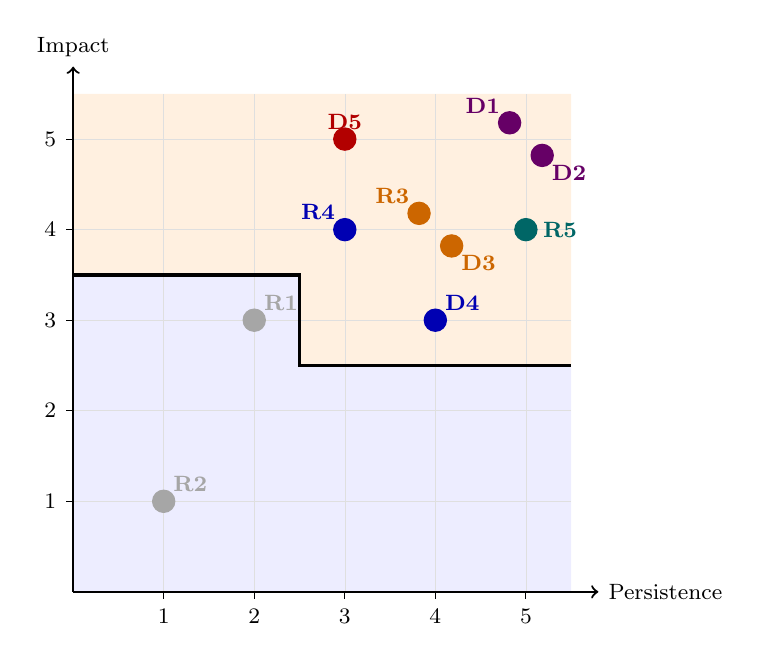
\begin{tikzpicture}[scale=1.15, font=\small]

  % --- Background zones ---
  \fill[orange!12]
    (0,3.5) -- (2.5,3.5) -- (2.5,2.5) -- (5.5,2.5)
    -- (5.5,5.5) -- (0,5.5) -- cycle;
  \fill[blue!7]
    (0,0) -- (5.5,0) -- (5.5,2.5) -- (2.5,2.5)
    -- (2.5,3.5) -- (0,3.5) -- cycle;

  % --- Grid ---
  \draw[gray!25, very thin, step=1] (0,0) grid (5.5,5.5);

  % --- Urgency curve (step polyline) ---
  \draw[very thick, black]
    (0,3.5) -- (2.5,3.5) -- (2.5,2.5) -- (5.5,2.5);

  % --- Axes ---
  \draw[->, thick] (0,0) -- (5.8,0)
    node[right, font=\footnotesize] {Persistence};
  \draw[->, thick] (0,0) -- (0,5.8)
    node[above, font=\footnotesize] {Impact};

  % --- X-axis ticks and labels ---
  \foreach \x in {1,2,3,4,5}{
    \draw (\x, 0) -- (\x,-0.08) node[below, font=\footnotesize] {\x};
  }
  % --- Y-axis ticks and labels ---
  \foreach \y in {1,2,3,4,5}{
    \draw (0,\y) -- (-0.08,\y) node[left, font=\footnotesize] {\y};
  }

  % ============================================================
  % POINTS (P = X-axis, I = Y-axis)
  % Full scale 1--5; points in the same cell slightly offset
  % ============================================================

  % D1 — P=5, I=5 (offset \u2197)
  \filldraw[violet!80!black] (4.82,5.18) circle (3.5pt);
  \node[violet!80!black, font=\footnotesize\bfseries, above left]
    at (4.82,5.18) {D1};

  % D2 — P=5, I=5 (offset \u2198)
  \filldraw[violet!80!black] (5.18,4.82) circle (3.5pt);
  \node[violet!80!black, font=\footnotesize\bfseries, below right]
    at (5.18,4.82) {D2};

  % R5 — P=5, I=4
  \filldraw[teal!80!black] (5,4) circle (3.5pt);
  \node[teal!80!black, font=\footnotesize\bfseries, right]
    at (5,4) {\;R5};

  % D5 — P=3, I=5
  \filldraw[red!70!black] (3,5) circle (3.5pt);
  \node[red!70!black, font=\footnotesize\bfseries, above]
    at (3,5) {D5};

  % R3 — P=4, I=4 (offset \u2197)
  \filldraw[orange!80!black] (3.82,4.18) circle (3.5pt);
  \node[orange!80!black, font=\footnotesize\bfseries, above left]
    at (3.82,4.18) {R3};

  % D3 — P=4, I=4 (offset \u2198)
  \filldraw[orange!80!black] (4.18,3.82) circle (3.5pt);
  \node[orange!80!black, font=\footnotesize\bfseries, below right]
    at (4.18,3.82) {D3};

  % R4 — P=3, I=4
  \filldraw[blue!70!black] (3,4) circle (3.5pt);
  \node[blue!70!black, font=\footnotesize\bfseries, above left]
    at (3,4) {R4};

  % D4 — P=4, I=3
  \filldraw[blue!70!black] (4,3) circle (3.5pt);
  \node[blue!70!black, font=\footnotesize\bfseries, above right]
    at (4,3) {D4};

  % R1 — P=2, I=3
  \filldraw[gray!70] (2,3) circle (3.5pt);
  \node[gray!70, font=\footnotesize\bfseries, above right]
    at (2,3) {R1};

  % R2 — P=1, I=1
  \filldraw[gray!70] (1,1) circle (3.5pt);
  \node[gray!70, font=\footnotesize\bfseries, above right]
    at (1,1) {R2};

\end{tikzpicture}
\caption{Urgency curve --- TPER issues by impact and persistence.
  The polyline separates issues to be fixed immediately (orange zone,
  above the curve) from those to be monitored in the next release
  (blue zone, below the curve).}
\label{fig:urgency-curve}
\end{figure}
% ================================================================

\newpage

% ================================================================
% DESIGN RECOMMENDATIONS --- Phase A Conclusion
% (from designrecco.tex with adaptations)
% ================================================================
\section{Design Recommendations}

\label{sec:design-recommendations}

The design recommendations presented in this section derive
directly from the systematic cross-referencing of results emerged from the heuristic
evaluation, field studies, and preliminary user testing. Each
recommendation is traceable to specific empirical evidence and guideline
violations, and is formulated in operational terms to guide
the implementation of the trainer-mode and the overall redesign
of the TPER ecosystem.

The recommendations are organized by macro-design themes (information
architecture, trainer modeà authentication, accessibility, errorà
support, multilingual, and progress monitoring), reflecting the main
intervention areas identified.

% ================================================================
% MACRO-AREA 1: INFORMATION ARCHITECTURE AND HOME PAGE
% ================================================================

\subsection{Redefinition of Information Architecture and Home Page}

\subsubsection{R1 -- Task-Oriented Home Page}
\label{rec:R1}

\textbf{Recommendation}: Redesign the \texttt{tper.it} home page
introducing a clear visual hierarchy that prioritizes primary actions
for the end user (subscription renewal, trip planning,
timetable consultation) over corporate news and secondary notices.

\textbf{Implementation}: Place the main CTAs in a prominent
block above the page fold, using generously sized buttons
(minimum 44$\times$44px for touch targets) with bold labels.
Corporate news and service notices should be moved to
a secondary section, placed after priority content.

\textbf{Supporting evidence}:
\begin{itemize}
    \item \textbf{Heuristic}: Violation G1 and G7 (homepage unclear,
    visual hierarchy absent).
    \item \textbf{User testing}: Maria B. (79 years) stated: "I don't even know where to start", completing 0 out of 5 tasks. Sergio M.
    (67 years) took 354 seconds for Task 1, blocked by
    disorientation on the homepage. Laura P. (70 years) commented:
    ``The interface is too cluttered, there is too much confusion'' [original Italian: ``L'interfaccia \`e troppo ingombrante, c'\`e troppa confusione''].
    Chris H. (34 years, high competence) took 226 seconds for
    Task 1, confirming the severity even for users with greater
    digital familiarity.
    \item \textbf{Field observation}: None of the TPER counter staff show
    the public website, a sign that the current home page is not perceived as
    a reliable starting point for user interaction.
\end{itemize}

\subsubsection{R2 -- Flat and Linear Information Architecture}
\label{rec:R2}

\textbf{Recommendation}: Restructure the site's information architecture
according to a flat model (flat IA), for the most frequent
transactional functions (purchase, renewal, discounts).

\textbf{Implementation}: Replace the current mixed menu with a
clear horizontal tab structure: \textit{Buy}, \textit{Plan},
\textit{Help}. Each section must present all
available operations on a single screen, avoiding dropdown submenus
that increase cognitive load.

\textbf{Supporting evidence}:
\begin{itemize}
    \item \textbf{Heuristic}: Violation G3 -- Confusing information
    architecture; labels use corporate terminology, the path to
    reach a subscription renewal requires more than three
    non-linear clicks.
    \item \textbf{User testing}: Sergio M. failed T1 and T4 due to
    the unintuitive navigation structure. Laura P. described
    the path to concessions as ``really dispersive'',
    accumulating 7 errors in T3 and T4. Chris H. (34 years, high
    competence) and Maria B. (79 years, minimal competence) both failed
    Task 3, confirming that the complexity of the information
    architecture affects users regardless of digital competence level.
\end{itemize}

\subsubsection{R3 -- Progressive Signposting in the Transactional Flow}
\label{rec:R3}

\textbf{Recommendation}: Introduce a progress indicator
(progress bar) in the purchase and subscription renewal flows,
to orient the user on the number of remaining steps.

\textbf{Implementation}: The progress bar must show:
\begin{enumerate}
    \item the total number of steps;
    \item the current step with a simple text description (e.g. "Step 2 of 4 -- Choose the subscription type");
    \item a graphical completion indicator (e.g. dashed line or
    fill).
\end{enumerate}
The component should be inserted as a static element at the top of each
transactional flow page.

\textbf{Supporting evidence}:
\begin{itemize}
    \item \textbf{Field observation}: The TPER counter operator has an average
    of 3--5 minutes for simple requests, a time window that
    becomes the most binding design constraint. No guided flow can
    exceed this threshold.
    \item \textbf{User testing}: Task 3 was failed by Maria B.
    and Chris H., with an average time spent of 555 s and 498 s respectively
    before abandonment or blocking error.
\end{itemize}


% ================================================================
% MACRO-AREA 2: TRAINER MODE AND CAREGIVER SUPPORT
% ================================================================

\subsection{Trainer-Mode and Support for Assisted Guidance}

\subsubsection{R4 -- Interface Duality (Trainer-Mode / User-Mode)}
\label{rec:R4}

\textbf{Recommendation}: Design a \textit{trainer-mode} that can be activated
via a visible toggle in the lower right corner of the screen,
allowing the intermediary to access guidance tools (contextual
tooltips, step-by-step walkthrough, element highlighting)
without modifying the interface structure for the end user.

\textbf{Implementation}: In trainer-mode:
\begin{itemize}
    \item explanatory labels (tooltips) will appear next to the
    interactive elements the trainer is explaining;
    \item the intermediary will have a step-by-step walkthrough with
    a progress indicator (current step, total steps);
    \item an ``explanation mode'' will be available that highlights with a
    colored border the area of the screen being explained.
\end{itemize}
The two views (trainer and user) must coexist on the same screen
(e.g. split view with side sidebar) during in-person assistance.

\textbf{Supporting evidence}:
\begin{itemize}
    \item \textbf{Heuristic}: Violation G9 and R5 -- catastrophic absence of
    activatable contextual support and no trainer-mode for guiding
    the vulnerable user in a structured and repeatable way.
    \item \textbf{Segmentation}: The three priority segments identify
    different training contexts and intermediary profiles (family member,
    operator, volunteer), requiring modular guidance tools.
    \item \textbf{Market Research}: Interviews with elderly commuters
    (Card \#1) revealed the dynamic of total delegation: the family member
    performs on behalf of the user. The trainer-mode must actively inhibit
    this pattern by shifting controls toward the end user.
\end{itemize}

\subsubsection{R5 -- Progress Persistence (Session Memory)}
\label{rec:R5}

\textbf{Recommendation}: Design a progress persistence system
that allows the user to save the training session state (which
flows have been completed, which step was reached in each flow)
and to resume it later from the same point, without having to start
over from scratch.

\textbf{Implementation}: At the first interruption -- browser close,
logout, or timeout -- the system must automatically save the session
state. On the next access, the user (or intermediary) resumes
automatically from where they left off. Persistence does not require
registration: it must work from the very first access in guest mode.

\textbf{Supporting evidence}:
\begin{itemize}
    \item \textbf{Market Research}: Interviews from Card \#1
    highlighted the frustration of intermediaries in having to repeat
    the same instructions without lasting results.
    \item \textbf{Association context}: Assistance center staff have extended time
    (longer sessions) but rarely leave written material with the user.
    Progress persistence allows resuming the session without starting from scratch.
\end{itemize}

\subsubsection{R6 -- Printable Post-Session Summary}
\label{rec:R6}

\textbf{Recommendation}: At the end of each training session, automatically generate
a summary of completed steps, with annotated screenshots
of key screens, to save as PDF or print.

\textbf{Implementation}: The summary must include:
\begin{enumerate}
    \item a bulleted list of operations performed;
    \item for each operation, the navigational path (e.g.
    ``Home $\rightarrow$ Buy $\rightarrow$ Monthly subscription $\rightarrow$ Payment'').
\end{enumerate}
The document must be formatted with a minimum 14pt font and high
contrast to be readable even by elderly users.

\textbf{Supporting evidence}:
\begin{itemize}
    \item \textbf{Associational context}: The staff at assistance centers
    rarely leaves material with the user at the end of the
    session. The printable summary fills this gap and provides an
    autonomous reference between one session and the next.
\end{itemize}


% ================================================================
% MACRO-AREA 3: AUTHENTICATION AND SPID
% ================================================================

\subsection{Redesign of Authentication: Guest Path}

\subsubsection{R7 -- Guest Path for Basic Operations}
\label{rec:R7}

\textbf{Recommendation}: Introduce a \textit{guest} path for
the renewal of impersonal subscriptions, Boost top-up, and fine
payment, requiring only the card number (or fiscal code
for fines), email address, and payment method, without
mandatory registration.

\textbf{Implementation}: The guest flow must:
\begin{enumerate}
    \item be visible as an option on the login screen
    (``Continue without registration'');
    \item require only the card number and email address (for
    sending the receipt) for renewals; add the fiscal code
    as verification for fines;
    \item redirect to the payment gateway without creating a permanent
    account.
\end{enumerate}
For operations requiring authentication (e.g. ISEE fare
concessions, nominative subscriptions), the system must show
a clear explanation of what data is needed, why, and how long
the procedure takes.

\textbf{Supporting evidence}:
\begin{itemize}
    \item \textbf{Heuristic}: Violation G4 and D5 -- mandatory
    registration is not accompanied by explanations or a guest
    alternative, making the platform inaccessible to the elderly target.
    \item \textbf{User testing}: Task 3 was failed by three
    subjects out of four (Laura P., Chris H., Maria B.) due to
    mandatory registration, regardless of digital competence level.
    \item \textbf{Competitor test (ATAC)}: Also on ATAC, the
    MyAtac registration blocked subjects with lower digital
    competence (Laura P. and Maria B.), while Chris H. completed only
    3 tasks out of 5. The data confirms that mandatory authentication
    is a cross-cutting critical point.
\end{itemize}



% ================================================================
% MACRO-AREA 4: COGNITIVE AND VISUAL ACCESSIBILITY
% ================================================================

\subsection{Cognitive and Visual Accessibility for Elderly and Vulnerable Users}

\subsubsection{R8 -- Large Text, High Contrast, and Clickable Areas}
\label{rec:R8}

\textbf{Recommendation}: Bring the entire site to WCAG 2.1 level
AA compliance, with particular emphasis on:
\begin{itemize}
    \item base text size not less than 16px (or 1rem);
    \item text/background contrast ratio minimum 4.5:1;
    \item clickable areas of at least 44x44px for touch;
    \item modalit\`a ad alto contrasto attivabile da un interruttore visibile
    in home page.
\end{itemize}

\textbf{Supporting evidence}:
\begin{itemize}
    \item \textbf{Heuristic}: Violation G10 and R3 -- small text size,
    insufficient contrast, clickable areas too small for smartphone
    use.
    \item \textbf{ISTAT data}: 72.5\% of 65--74 year-olds use the Internet,
    a share that drops to 35.7\% among over-75s. Digital competence levels at least
    stand at 27.4\% in the 65--74 age group.
    \item \textbf{User testing}: Maria B. (79 years) was unable to distinguish
    an interactive button from a static text string, due to
    insufficient contrast and size.
\end{itemize}

\subsubsection{R9 -- Content with an Encouraging and Inclusive Tone}
\label{rec:R9}

\textbf{Recommendation}: Design the site's content with an encouraging,
reassuring, and non-paternalistic tone, that reduces the digital
anxiety of the vulnerable user and motivates them to continue independently.
The language must convey "you can do it" rather than "this is
an ISEE form".

\textbf{Implementation}: Each flow must include:
\begin{enumerate}
    \item a motivational welcome message at startup (e.g. ``You'll see,
    just one step at a time -- shall we start together?" not just "Proceed");
    \item short texts, in active and positive form (``Fill in your data''
    not "Data must be filled in");
    \item reinforcement micro-text after each completed step (``Perfect,
    this one is done! Let's move on to the next");
    \item a consistent tone throughout the site: friendly but respectful,
    never childish.
\end{enumerate}
Institutional and legal content (fares, regulations) must remain
accurate but be framed by the encouraging tone. This is not about
"simplifying vocabulary" but about designing the emotional relationship
with the user through words.

\textbf{Supporting evidence}:
\begin{itemize}
    \item \textbf{User testing}: Maria B. (79 years) stated: "I don't even know
    where to start" -- the problem is not lexical but a
    lack of emotional guidance to accompany her in the first step.
    \item \textbf{User testing}: Chris H. (Test \#3 TPER) requested
    "clearer guidance" not in a technical sense but as a need for
    accompaniment to make him feel safe in an unfamiliar
    linguistic and cultural context.
    \item \textbf{Criteri di valutazione}: Explicitly seek
    the "Find a tone and a message" (p.98) and that
    "tone and messages are important for motivation" (p.89).
\end{itemize}


% ================================================================
% MACRO-AREA 5: ERROR SUPPORT AND FEEDBACK
% ================================================================

\subsection{Error Support and Contextual Feedback}

\subsubsection{R10 -- Expansive and Guided Error Messages}
\label{rec:R10}

\textbf{Recommendation}: Replace generic error messages
("Error -- try again") with expansive messages explaining:
\begin{enumerate}
    \item what happened (e.g. "The credit card was declined");
    \item why it happened (e.g. "The CVV code entered is incorrect");
    \item how to resolve (e.g. "Check the 3-digit code on the back of the
    card");
    \item alternative actions (e.g. "Try another card or PayPal").
\end{enumerate}

\textbf{Implementation}: Error messages must be displayed in
a high-contrast colored box (text on light red background with a warning
icon), positioned immediately above the field that generated
the error (inline error).

\textbf{Supporting evidence}:
\begin{itemize}
    \item \textbf{Heuristic}: Violation G9 -- the system does not guide the user
    in recovering from common errors (failed payment, expired subscription),
    generating call center calls and counter queues.
    \item \textbf{User testing}: Laura P. and Chris H. abandoned
    the purchase flow after an unexplained error, without attempting
    to try again.
\end{itemize}

\subsubsection{R11 -- Preventive Document Checklist}
\label{rec:R11}

\textbf{Recommendation}: Insert in every flow that requires document
upload (discounts, discounted subscription renewal) a preventive
checklist of all required documents, with visual examples and the option
to download a summary form.

\textbf{Implementation}: The checklist must be shown before starting
the upload flow, with a check icon that the user can activate to mark
each document as "in possession". At the end, the system must generate a
list of missing ones and provide instructions on how to obtain them.

\textbf{Supporting evidence}:
\begin{itemize}
    \item \textbf{Field observation}: Elderly users often do not know in
    advance which documents to bring and must return to the counter on a
    subsequent visit.
    \item \textbf{Heuristic}: The absence of a preventive checklist increases
    counter returns and generates a cycle of dependency on physical
    service.
\end{itemize}


% ================================================================
% MACRO-AREA 6: MULTILINGUAL AND FOREIGN SUPPORT
% ================================================================

\subsection{Multilingual Support for Foreign Users}

\subsubsection{R12 -- English and Arabic Version of Transactional Flows}
\label{rec:R12}

\textbf{Recommendation}: Provide complete translation in English and Arabic
(the two most spoken foreign languages in Emilia-Romagna) of all transactional
flows (purchase, renewal, discounts) and main information
pages (timetables, routes, notices).

\textbf{Implementation}: Language selection must be persistent
(remembered via cookie) and accessible from a fixed selector in the header.
Translations must be professional, not automatic, and validated by
native speakers. For technical texts (SPID, ISEE), provide a simplified
language explanation alongside.

\textbf{Supporting evidence}:
\begin{itemize}
    \item \textbf{User testing}: Chris H. (34 years, English native speaker) failed
    Tasks 3, 4, and 5 due to the language barrier, despite
    high digital competence.
    \item \textbf{ISTAT data}: As of 1\textdegree\ January 2025, 5,422,000
    foreign nationals reside in Italy, with a strong concentration in Emilia-Romagna.
    \item \textbf{Segment [S2] -- The foreign worker}: Introduces
    a double barrier (linguistic and systemic) that no other
    combination presents.
\end{itemize}



% ================================================================
% MACRO-AREA 7: PROGRESS MONITORING
% ================================================================

\subsection{Progress Monitoring and Self-Efficacy}

\subsubsection{R13 -- Progress Dashboard for the Intermediary}
\label{rec:R13}

\textbf{Recommendation}: In trainer-mode, provide the intermediary with a
dashboard displaying:
\begin{enumerate}
    \item the percentage of tasks completed by the user across various flows;
    \item the number of errors made in each flow (aggregated);
    \item an estimate of average time spent per flow.
\end{enumerate}

\textbf{Implementation}: Data must be collected anonymously
and resettable with the user's consent. The dashboard must include a
simplified Likert scale (3 levels: positive, neutral, negative) that the intermediary can have
the user fill out at session end to measure perceived self-efficacy.

\textbf{Supporting evidence}:
\begin{itemize}
    \item \textbf{Business goals}: Progress monitoring is explicitly
    required in the tool's objectives.
    \item \textbf{User testing}: The average SUS of the four TPER tests
    was 37.50/100, well below the acceptability threshold;
    progress monitoring also serves to verify the effectiveness of the redesign.
\end{itemize}


% ================================================================
% RECOMMENDATIONS SUMMARY
% ================================================================
\newpage
\subsection{Summary of Recommendations}

\begin{table}[htbp]
\centering
\caption{Overview of design recommendations by macro-area}
\label{tab:recommendations-summary}
\begin{tabular}{|p{2.8cm}|p{10cm}|}
\hline
\textbf{Macro-area} & \textbf{Recommendations} \\
\hline
Architecture and Home Page & R1 -- Task-oriented home page \\
& R2 -- Flat and linear IA \\
& R3 -- Progressive signposting \\
\hline
Trainer-mode and support & R4 -- Interface duality \\
& R5 -- Progress persistence \\
& R6 -- Printable summary \\
\hline
Authentication & R7 -- Guest path for basic operations \\
\hline
Accessibility & R8 -- Large text and high contrast \\
& R9 -- Encouraging tone content \\
\hline
Error support & R10 -- Expansive error messages \\
& R11 -- Preventive document checklist \\
\hline
Multilingual & R12 -- English and Arabic versions \\
\hline
Progress monitoring & R13 -- Intermediary dashboard \\
\hline
\end{tabular}
\end{table}

\noindent The recommendations listed above constitute the baseline for the
prototyping and development phase of the trainer-mode. It is recommended to
adopt an iterative approach (design--prototype--test--refine) with the
direct involvement of the identified user segments (elderly commuter,
foreign worker) to validate
the effectiveness of the proposed solutions.

\begin{center}
    {\color{primaryColor}\Large\bfseries Persona and Use Case Card} \\[4pt]
    {\color{secondaryColor}\normalsize Phase B --- Feasibility Study} \\[4pt]
    {\color{secondaryColor}\small  This \textit{persona} is the \textbf{protagonist} (i.e., the person for whom we are designing the new tool; this \textit{persona} must be 100\% satisfied by the design; unless there are good reasons, only one \textit{persona} in the cast is the protagonist).}

\vspace{0.3cm}
{\color{borderColor}\hrule}
\vspace{0.5cm}

% ================================================================
% ROW 1: PHOTO + PERSONAL DATA
% ================================================================

\begin{minipage}[t]{0.25\textwidth}
    \centering
    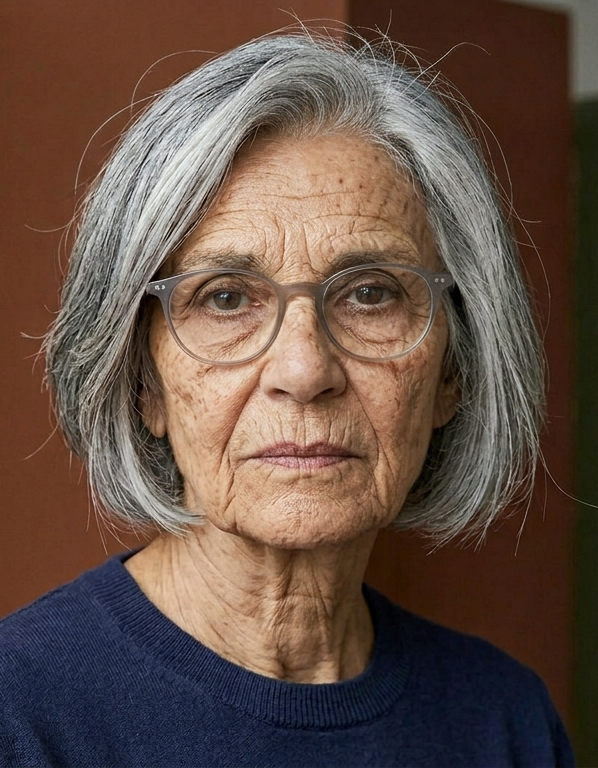
\includegraphics[width=\textwidth,height=5cm,keepaspectratio]
    {images/fatima.png}
    \vspace{0.2cm}
\end{minipage}
\hfill
\begin{minipage}[t]{0.70\textwidth}
    \begin{tcolorbox}[personabox]
        \textbf{\large Fatima Benali}\label{persona:fatima_benali} \\[4pt]
        {\color{secondaryColor}\small\textbf{Meaningful quote:}
        \textit{"I don't understand written Italian words,
        but I know perfectly well which bus to take and where to get off"}} \\[4pt]
        {\color{secondaryColor}\small\textbf{Corresponding segment:}
        Elderly foreigner (68 years old, Moroccan origin,
        literate in Arabic but illiterate in written Italian,
        minimal digital competence, frequent TPL user)}
    \end{tcolorbox}
\end{minipage}

\vspace{0.3cm}

% ================================================================
% PERSONA DESCRIPTION (Basic Facts)
% ================================================================

\begin{tcolorbox}[base]
    \textbf{Persona description} \\[4pt]
    {\small
    \textbf{Età:} 68 anni \hfill
    \textbf{Gender:} Female \hfill
    \textbf{Nazionalità:} Moroccan, resident in Italy for 22 years
    \\[2pt]
    \textbf{Residence:} Bologna, Pilastro district \hfill
    \textbf{Marital status:} Married \\[2pt]
    \textbf{Education:} Primary school completed in Morocco
    in Arabic. She can read and write in Arabic,
    but has never received any education in Italian. \\[2pt]
    \textbf{Language proficiency:} Elementary oral Italian
    (sufficient for routine interactions: market, doctor,
    counter). Written Italian: none. She does not recognize the
    letters of the Latin alphabet and is unable to read
    any Italian word, not even the most common ones.
    She reads and writes correctly in Arabic: she uses WhatsApp
    in Arabic to communicate with family in Morocco
    and with the Al-Amal center group. \\[2pt]
    \textbf{Relevant physical issues:} Mild low vision
    corrected with prescription glasses. Fine motor skills within normal range
    for her age, with no significant limitations to the hands.
    Rapid visual fatigue in front of screens. \\[2pt]
    \textbf{Digital profile:} She owns an Android smartphone
    bought by her son. She uses it daily for
    video calls and WhatsApp messages in Arabic with
    family in Morocco and with friends from the Al-Amal center.
    She has never browsed a website, does not know what
    a browser is, does not know the concept of SPID or ISEE.
    She has never entered data in an online form. \\[2pt]
    \textbf{TPL usage:} She uses TPER transport almost every day
for over twenty years to reach the market, the neighborhood
mosque, and the Al-Amal community center.
She has a discounted monthly subscription that until now
her son Karim renewed at the counter every month.
Since the Al-Amal center started a digital
assistance desk with a dedicated volunteer,
Fatima has turned to her for online procedures.
She knows perfectly lines, stops, connections,
and fare zones of the area where she lives.
    }
\end{tcolorbox}

% ================================================================
% BACKGROUND AND PSYCHOLOGICAL CHARACTERISTICS
% ================================================================

% ================================================================
% BACKGROUND -- replace the paragraphs about Karim and the context
% ================================================================

\begin{tcolorbox}[base]
    \textbf{Background and psychological characteristics} \\[4pt]
    {\small
    Fatima arrived in Italy in 2003, joining her husband
    Rachid (retired factory worker) already living in Bologna.
    She has always been a homemaker and raised three children
    in Italy: the eldest, Karim (38 years old), works in a
    logistics warehouse with night shifts; the second,
    Nadia (34 years old), lives in Modena with her own family;
    the youngest, Youssef (28 years old), studies engineering
    in Bologna and lives away from home. For years it was Karim
    who handled all the family's bureaucratic procedures,
    often in a hurry between shifts. \\[4pt]

    Fatima can read and write in Arabic, but has never
    learned the Latin alphabet: she grew up in Morocco where
    education was in Arabic, and in 22 years of life in Italy
    she has never attended a structured language course.
    She understands spoken Italian in everyday situations,
    but in front of a written Italian word it is like
    being in front of an unknown code:
    she cannot decipher even individual letters.
    She has built an autonomous and dignified life through
    an extraordinary \textbf{visual and spatial memory}:
    she recognizes places by the shape of buildings, shops
    by the colors of signs, buses by number ---
    which she has learned to recognize as a visual form,
    not as a linguistic symbol.
    She can navigate all of Bologna without reading a sign. \\[4pt]

    The turning point in Fatima's digital life
    was the Al-Amal center. About a year ago,
    the association started a \textbf{digital
    assistance desk} run by Sara, a
    28-year-old second-generation volunteer,
    who speaks Arabic and Italian and knows well
    the local bureaucratic procedures. Sara does not
    replace Fatima: she sits next to her, points
    at the screen, waits for her to touch.
    In this structured context --- sitting at a
    table, without Karim's rush between shifts
    --- Fatima feels safe and can
    concentrate. The center has become the place
    where Fatima learns, through imitation and repetition,
    what outside the center seems inaccessible to her. \\[4pt]

    Unlike Liliana, who actively feels the
    frustration of her own digital dependence,
    Fatima lives it with \textbf{pragmatic resignation}:
    she considers it normal for someone to help her with these things,
    just as she helps the other women at the center
    when it comes to navigating the city by transport.
    She does not yet perceive digital autonomy as a
    desirable goal. However, when Sara shows her
    that she could renew the subscription on her own
    without waiting for anyone, she reacts with genuine curiosity:
    \textit{"But can you really do it on your own?
    No one ever told me that"}.
    }
\end{tcolorbox}

\vspace{0.3cm}

% ================================================================
% C&A DIAGRAM
% ================================================================

\begin{tcolorbox}[personabox]
    \textbf{Competences and Abilities Chart (C\&A Diagram)} \\[4pt]
    {\small
    }

    \vspace{0.3cm}

    \begin{center}
    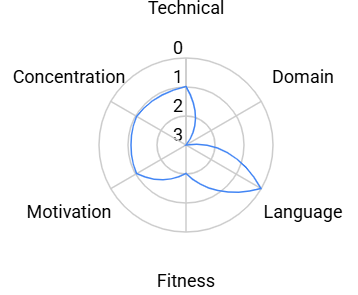
\includegraphics[width=0.85\textwidth]{images/fatima_chart.png}
    \end{center}

    \vspace{0.2cm}

    \begin{center}
    \renewcommand{\arraystretch}{1.3}
    \begin{tabular}{|l|c|c|}
        \hline
        \textbf{Dimension} & \textbf{Score (1--5)} & \textbf{Indicator} \\
        \hline
        Technical competence &
       \textbf{2} &
        \cellcolor{gray!10} \makebox[50pt]{\rule{10pt}{10pt}\rule{10pt}{10pt}\color{lightgray}\rule{10pt}{10pt}\rule{10pt}{10pt}\rule{10pt}{10pt}} \\
        \hline
        Domain competence &
        \textbf{4} &
        \cellcolor{gray!10} \makebox[50pt]{\rule{10pt}{10pt}\rule{10pt}{10pt}\rule{10pt}{10pt}\rule{10pt}{10pt}\color{lightgray}\rule{10pt}{10pt}} \\
        \hline
        Language competence &
        \textbf{1} &
        \cellcolor{gray!10} \makebox[50pt]{\rule{10pt}{10pt}\color{lightgray}\rule{10pt}{10pt}\rule{10pt}{10pt}\rule{10pt}{10pt}\rule{10pt}{10pt}} \\
        \hline
        Physical and visual ability &
        \textbf{3} &
        \cellcolor{gray!10} \makebox[50pt]{\rule{10pt}{10pt}\rule{10pt}{10pt}\rule{10pt}{10pt}\color{lightgray}\rule{10pt}{10pt}\rule{10pt}{10pt}} \\
        \hline
        Motivation &
        \textbf{2} &
        \cellcolor{gray!10} \makebox[50pt]{\rule{10pt}{10pt}\rule{10pt}{10pt}\color{lightgray}\rule{10pt}{10pt}\rule{10pt}{10pt}\rule{10pt}{10pt}} \\
        \hline
        Concentration &
        \textbf{2} &
        \cellcolor{gray!10} \makebox[50pt]{\rule{10pt}{10pt}\rule{10pt}{10pt}\color{lightgray}\rule{10pt}{10pt}\rule{10pt}{10pt}\rule{10pt}{10pt}} \\
        \hline
    \end{tabular}
    \end{center}

    \vspace{0.2cm}
    {\small \textbf{Legend:} \rule{10pt}{10pt} = achieved value \hfill \color{lightgray}\rule{10pt}{10pt}\color{black} = not achieved value}

    \vspace{0.3cm}
    {\small \textit{Note: Unlike Liliana (motivation 3),
    who actively feels the frustration of dependence,
    Fatima experiences dependence as a normal and inevitable condition.
    Her high domain competence (4) is instead a fundamental
    design resource: Fatima already knows lines,
    stops, and fare zones. If the design manages to hook into
    what she already knows --- line numbers, zone
    icons, stop colors --- the learning curve
    is drastically reduced even in the presence of a
    structural language barrier.}}
\end{tcolorbox}

\vspace{0.3cm}

% ================================================================
% ADDITIONAL INTERESTING DETAILS
% ================================================================

% ================================================================
% ADDITIONAL INTERESTING DETAILS -- updated to Al-Amal context
% ================================================================

\begin{tcolorbox}[base,colback=backgroundColor!50]
    \textbf{Additional interesting details} \\[4pt]
    {\small
    \begin{itemize}[leftmargin=*]
        \item Fatima reads and writes fluently in Arabic
        and uses WhatsApp every day to message with
        family still in Morocco and with friends
        from the Al-Amal center. But in front of a screen
        in Italian she is completely disoriented:
        she does not recognize the letters, she cannot rely
        on text to orient herself. She recognizes, however, the TPER
        logo, line colors, and bus numbers
        as visual forms consolidated by daily
        experience. Her mind processes Italian
        through images, not text.

        \item Al-Amal's digital help desk has a
        desktop computer with a stable connection and
        Sara who receives on Tuesday and Thursday afternoons.
        Fatima has learned to show up on Sara's
        days when she needs to do "computer stuff".
        She has already completed two sessions: in the first
        she learned to open the browser, in the second
        she reached the TPER homepage. The subscription
        renewal will be the third session.

        \item At the Al-Amal center she learned to use
        WhatsApp by watching other women do it,
        without anyone explaining it to her in words.
        She learns through visual imitation and repetition,
        not through verbal instruction: the most effective
        learning model for her is
        "watch and repeat", not "read and follow
        instructions". Sara has adapted
        her own teaching method
        to this style: show first, speak later.

        \item She keeps her important documents
        (residence permit, health card,
        TPER subscription) in a transparent envelope
        sorted by color and size. She does not read
        labels: she recognizes documents by their
        shape, color, and photo.
        Sara suggested she always bring
        the envelope to sessions: the TPER card
        will be the starting point for the renewal
        flow.
    \end{itemize}
    }
\end{tcolorbox}

% ================================================================
% USE CASE #1 (Renewal Scenario - Guided Training Session)
% ================================================================
\begin{tcolorbox}[sectionbox,colback=primaryColor!10]
    \textbf{Use Case description \#1: Guided training session for monthly subscription renewal}
\end{tcolorbox}

\vspace{0.3cm}

% --- Use Case Narrative (technical, Scenari.pdf compliant) ---
\begin{tcolorbox}[base]
    {\small
    \textbf{Scenario:} User (technical competence 2/5, language competence 1/5, illiterate in Latin alphabet) attempts monthly subscription renewal via browser in a training session with a human trainer present.

    \textbf{Objective:} Renew TPER monthly subscription via web, completing the procedure without the trainer taking control of the device.

    \textbf{Sequence:}
    \begin{enumerate}
        \item The user opens the browser and types \texttt{tper.it}: a practiced operation, completed successfully in 10 sec.
        \item The homepage presents a dense layout (banners, news, carousel). The user stares at the screen without recognizing visual anchor points. The trainer physically points: "Here."
        \item The user clicks by spatial imitation. The link redirects to \texttt{solweb.tper.it} without notification: interface, colors, and layout change entirely. No warning.
        \item The system requests registration: a 6-field form in Italian. The trainer reads and orally translates each field.
        \item Fiscal Code field: the user takes out the health card but cannot locate the requested data. The trainer physically indicates the position on the card and dictates the 16 characters.
        \item Accumulated registration time: 7 minutes ($\sim$50\% of the session). When the system requests the ``Mi Muovo'' card number, the user cannot find it on the card. The trainer indicates the data.
        \item Typing error on the card number: the system generates an error message in Italian. The user cannot decipher the message and does not know how to correct it. The trainer takes the mouse and corrects.
        \item At payment, the trainer enters the credit card details. The user only presses the final confirmation button.
    \end{enumerate}

    \textbf{Outcome:} Renewal completed (operational success). The user acquires no reproducible skills: the trainer substituted the user in 4 out of 8 steps. The training failure is systemic: mandatory registration consumes attentional resources before the main task.

    \textbf{Times:} 15 minutes total (7 minutes registration + 8 minutes renewal). Registration consumes 50\% of the time on a step unnecessary for the task.
    }
\end{tcolorbox}

% ================================================================
% CONCLUDING CONSIDERATIONS --- IMPACT ON DESIGN
% ================================================================
\begin{tcolorbox}[sectionbox,colback=primaryColor!10]
    \textbf{Concluding considerations --- Impact of persona and use case on design}
\end{tcolorbox}

\vspace{0.3cm}

\begin{tcolorbox}[base]
    {\small
    \textbf{Impact of persona Fatima Benali on design:} \\[4pt]
    Fatima is the only persona in the cast who does not read the Latin alphabet (language competence 1/5, concentration 2/5). Her profile highlights the following design requirements:

    \begin{itemize}[leftmargin=*]
        \item \textbf{RF-01 --- Iconographic, non-textual interface:}
        Every label, button, and message in Italian is unreadable to the user. The interface must communicate via icons, photographs, colors, and visual references to the real public transport experience, not via text.

        \item \textbf{RF-02 --- Learning support through visual imitation:}
        The user learns through "watch and repeat", not through "read and follow instructions". Every flow must be executable by spatial imitation, without requiring textual decoding.

        \item \textbf{RF-03 --- Visual recognition of documents:}
        When the system requests data from a physical document, it must show a visual reproduction of the document with a graphical indication (arrow/highlighter) of the exact position of the data.

        \item \textbf{RF-04 --- Minimum path to the main task:}
        Every non-essential preliminary step (e.g. registration) consumes scarce attentional resources. The flow must minimize steps before the target operation.
    \end{itemize}
    }
\end{tcolorbox}

\vspace{0.3cm}

\begin{tcolorbox}[base]
    {\small
    \textbf{Impact of Use Case \#1 on design:} \\[4pt]
    Even with a dedicated human trainer, the current system prevents the transfer of skills to the user. Requirements emerged:

    \begin{itemize}[leftmargin=*]
        \item \textbf{RF-05 --- Visual continuity across platforms:}
        The transition from \texttt{tper.it} to \texttt{solweb.tper.it} must be signaled to the user with a context indicator (e.g. overlay "You are about to move to the purchase site"). The interface must maintain visual continuity elements (colors, logo, familiar layout).

        \item \textbf{RF-06 --- Guest flow for simple operations:}
        Mandatory registration for renewal consumes 50\% of session time and all the user's attentional capacity. Simple operations (renewal, verification) must be accessible without registration.

        \item \textbf{RF-07 --- Visual filling support:}
        Fields that require data from physical documents (card number, fiscal code) must be accompanied by an image of the document with a visual indication of the required data.

        \item \textbf{RF-08 --- Non-catastrophic errors:}
        Error messages must use icons and non-verbal language to communicate the nature of the problem to users who cannot read the interface language. Red color should be reserved for actual blocks, not for typos.

        \item \textbf{RF-09 --- Trainer mode with guidance tools:}
        The system must offer a mode that allows a trainer (human or digital) to highlight elements, dictate steps, and co-navigate without physically taking control of the device.
    \end{itemize}
    }
\end{tcolorbox}

\vspace{0.3cm}

\end{center}

\begin{center}
    {\color{primaryColor}\Large\bfseries Persona and Use Case Card} \\[4pt]
    {\color{secondaryColor}\normalsize Phase B --- Feasibility Study} \\[4pt]
    {\color{secondaryColor}\small This persona is not the protagonist (i.e., is not the person for whom we are designing the new tool; is a
supporting cast member who must nevertheless be taken into account to ensure an inclusive design).}
\end{center}

\vspace{0.3cm}
{\color{borderColor}\hrule}
\vspace{0.5cm}

% ================================================================
% ROW 1: PHOTO + PERSONAL DATA
% ================================================================

\begin{minipage}[t]{0.25\textwidth}
    \centering
    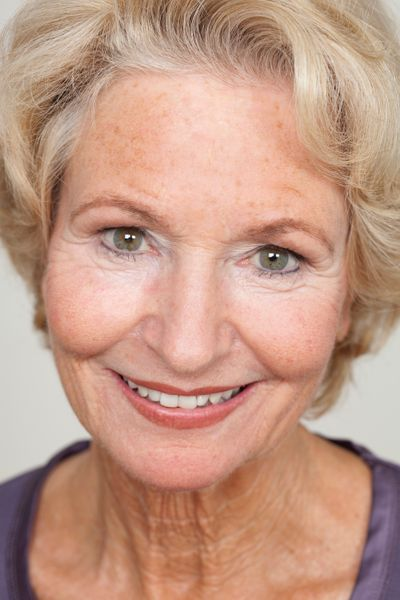
\includegraphics[width=\textwidth,height=5cm,keepaspectratio]{images/liliana.jpg}
    \vspace{0.2cm}
\end{minipage}
\hfill
\begin{minipage}[t]{0.70\textwidth}
    \begin{tcolorbox}[personabox]
        \textbf{\large Liliana Roversi} \\[4pt]
        {\color{secondaryColor}\small\textbf{Meaningful quote:} \textit{"I don't even know where to start, as far as I'm concerned my daughter has to do these things."}} \\[4pt]
        {\color{secondaryColor}\small\textbf{Corresponding segment:} Elderly commuter (over 75, minimal digital competence)}
    \end{tcolorbox}
\end{minipage}

\vspace{0.3cm}

% ================================================================
% PERSONA DESCRIPTION (Basic Facts)
% ================================================================

\begin{tcolorbox}[base]
    \textbf{Persona description} \\[4pt]
    {\small
    \textbf{Età:} 79 years \hfill
    \textbf{Gender:} Female \hfill
    \textbf{Nazionalità:} Italiana \\[2pt]
    \textbf{Residence:} Bologna, San Donato district (suburbs) \hfill
    \textbf{Marital status:} Widow, lives alone \\[2pt]
    \textbf{Education:} Elementary school diploma \\[2pt]
    \textbf{Relevant physical issues:} Presbyopia (uses reading glasses), hand arthritis that reduces fine motor skillsà fine, reduced mobilityà (walks with a cane for long journeys). \\[2pt]
    \textbf{Digital profile:} She owns a smartphone given to her by her daughter, but uses it exclusively for passive scrolling on Facebook (family photos) and WhatsApp calls. She has never used a browser for active navigation, has never filled in an online form. During tests, an initial orientation phase on the computer trackpad was necessary. \\[2pt]
    \textbf{TPL usage:} TPER user for over 40 years. She knows well the lines, stops, and fare zones from physical experience. She used to buy tickets at the newsstand and renew the subscription at the TPER counter in the station. Since many services have migrated online, she depends entirely on her daughter for every digital operation.
    }
\end{tcolorbox}

% ================================================================
% BACKGROUND AND PSYCHOLOGICAL CHARACTERISTICS
% ================================================================

\begin{tcolorbox}[base]
    \textbf{Background and psychological characteristics} \\[4pt]
    {\small
    Liliana was born and raised in Bologna, worked for 35 years as a school aide in a neighborhood elementary school. She retired 14 years ago. Her husband, a former railway worker, passed away 10 years ago; since then she has lived alone in a third-floor apartment without an elevator. She has two children: her eldest daughter, Elena (45 years old, municipal employee), lives in a neighboring town and visits her every Tuesday and Saturday; her younger son, Marco (41 years old), lives in Milan and returns to Bologna once a month. \\[4pt]

    Liliana is a proud woman accustomed to self-sufficiency: she has always managed the home, finances, and bureaucratic procedures independently. Her dependence on her daughter for digital operations is for her a source of strong frustration and shame. She declared: ``\textit{My daughter already has her own problems, I don't want to be a burden}''. \\[4pt]

    Psychologically, Liliana shows a deep \textbf{gap between motivation and self-efficacy}: she wants to learn, but every failed attempt reinforces the belief that she is ``not cut out'' for technology. She fears ``breaking something'' or ``causing damage'' if she clicks in the wrong place. She prefers not to try rather than make a mistake and feel humiliated. \\[4pt]

    She is a methodical and patient person in real life (she loves gardening and cooking, activities that require precision and repetition), but the digital environment disorients her: the density of information, multiple choices, and lack of a ``tactile'' physical path cause her anxiety and decision paralysis.
    }
\end{tcolorbox}

\vspace{0.3cm}

% ================================================================
% C&A DIAGRAM (Radar chart -- Competences and Abilities)
% ================================================================

\begin{tcolorbox}[personabox]
    \textbf{Competences and Abilities Chart (C\&A Diagram)} \\[4pt]
    {\small
    Each dimension is rated on a scale from 1 (very low) to 5 (very high). \\
    Liliana's scores reflect the profile that emerged from user tests and field observations.
    }

    \vspace{0.3cm}

    \begin{center}
    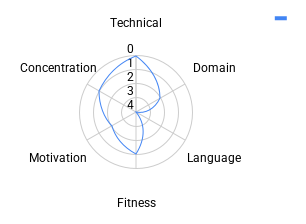
\includegraphics[width=0.85\textwidth]{images/liliana_chart.png}
    \end{center}

    \vspace{0.2cm}

    \begin{center}
    \renewcommand{\arraystretch}{1.3}
    \begin{tabular}{|l|c|c|}
        \hline
        \textbf{Dimension} & \textbf{Score (1--5)} & \textbf{Indicator} \\
        \hline
        Technical competence &
        \textbf{1} &
        \cellcolor{gray!10} \makebox[50pt]{\rule{10pt}{10pt}\color{lightgray}\rule{10pt}{10pt}\rule{10pt}{10pt}\rule{10pt}{10pt}\rule{10pt}{10pt}} \\
        \hline
        Domain competence &
        \textbf{3} &
        \cellcolor{gray!10} \makebox[50pt]{\rule{10pt}{10pt}\rule{10pt}{10pt}\rule{10pt}{10pt}\color{lightgray}\rule{10pt}{10pt}\rule{10pt}{10pt}} \\
        \hline
        Language competence &
        \textbf{5} &
        \cellcolor{gray!10} \makebox[50pt]{\rule{10pt}{10pt}\rule{10pt}{10pt}\rule{10pt}{10pt}\rule{10pt}{10pt}\rule{10pt}{10pt}} \\
        \hline
        Physical and visual ability &
        \textbf{2} &
        \cellcolor{gray!10} \makebox[50pt]{\rule{10pt}{10pt}\rule{10pt}{10pt}\color{lightgray}\rule{10pt}{10pt}\rule{10pt}{10pt}\rule{10pt}{10pt}} \\
        \hline
        Motivation &
        \textbf{3} &
        \cellcolor{gray!10} \makebox[50pt]{\rule{10pt}{10pt}\rule{10pt}{10pt}\rule{10pt}{10pt}\color{lightgray}\rule{10pt}{10pt}\rule{10pt}{10pt}} \\
        \hline
        Concentration &
        \textbf{2} &
        \cellcolor{gray!10} \makebox[50pt]{\rule{10pt}{10pt}\rule{10pt}{10pt}\color{lightgray}\rule{10pt}{10pt}\rule{10pt}{10pt}\rule{10pt}{10pt}} \\
        \hline
    \end{tabular}
    \end{center}

    \vspace{0.2cm}
    {\small \textbf{Legend:} \rule{10pt}{10pt} = achieved value \hfill \color{lightgray}\rule{10pt}{10pt}\color{black} = not achieved value}
\end{tcolorbox}

\vspace{0.3cm}

% ================================================================
% ADDITIONAL INTERESTING DETAILS
% ================================================================

\begin{tcolorbox}[base,colback=backgroundColor!50]
    \textbf{Additional interesting details} \\[4pt]
    {\small
    \begin{itemize}[leftmargin=*]
        \item Liliana has a notebook where her daughter writes ``the instructions'' for digital operations, but every time the site changes (even slightly) the instructions are no longer useful and she freezes.
        \item She still keeps all the old stamped paper tickets in a drawer: for her the ``ticket'' is a physical object, not a digital code.
        \item She talks on the phone with her son in Milan every evening, but has never tried to have anything explained about the smartphone over the phone --- ``I wouldn't understand anyway''.
        \item On Sunday mornings she goes to mass at the neighborhood parish, where she stops to talk with other elderly women from the neighborhood. Many share her same digital frustration, but none know how to overcome it.
    \end{itemize}
    }
\end{tcolorbox}

\newpage

% ================================================================
% USE CASE #1: «The phantom transition»
% ================================================================

\begin{tcolorbox}[sectionbox,colback=primaryColor!10]
    \textbf{Use Case description \#1: Attempted monthly subscription renewal --- the phantom transition between tper.it and solweb.tper.it}
\end{tcolorbox}

\vspace{0.3cm}

% --- Narrative ---
\begin{tcolorbox}[base]
    {\small
    \textbf{Scenario:} User (technical competence 1/5, concentration 2/5) attempts monthly subscription renewal via web in complete autonomy. The usual intermediary (daughter) is not available. Deadline: tomorrow.

    \textbf{Objective:} Renew the TPER monthly subscription via web without human assistance.

    \textbf{Sequence:}
    \begin{enumerate}
        \item The user opens the browser, types \texttt{tper.it} in the Google search bar instead of the address bar: interface recognition error. On the second attempt she reaches the homepage.
        \item The homepage presents news, notices, banners, and carousel without a visual hierarchy between informative content and transactional action. The user scans the page for 45 sec before finding the ``Subscriptions'' item in the top menu.
        \item The user clicks ``Subscriptions'' $\rightarrow$ ``Monthly'' $\rightarrow$ ``Purchase''. The link redirects to \texttt{solweb.tper.it} without notification. The interface changes completely (colors, layout, domain).
        \item The system requires login. The user does not have an account. She looks for a ``Continue without registration'' button: absent.
        \item The user attempts ``Register'': a form with 6+ mandatory fields (name, surname, email, password, confirmation, terms). She tries to fill it in, makes mistakes, deletes, retries for 5 minutes.
        \item After yet another error, the user closes the browser. She contacts the intermediary: ``I couldn't do it. Will you do it for me?''
    \end{enumerate}

    \textbf{Barriers:}
    \begin{itemize}
        \item Address bar vs. search bar recognition (technical competence 1/5).
        \item Transition \texttt{tper.it} $\rightarrow$ \texttt{solweb.tper.it} not signaled: platform switch without context.
        \item No guest path: mandatory registration even for simple operations.
        \item Extended registration form: 6+ fields, password complexity requirements not communicated.
        \item Generic error: the system reports the error but does not indicate how to correct it.
    \end{itemize}

    \textbf{Outcome:} Operation not completed. The intermediary performs the task on behalf of the user. Dependency cycle perpetuated. No skills transferred.

    \textbf{Times:} 15 minutes autonomous attempt + 10 minutes intermediary intervention.
    }
\end{tcolorbox}

\vspace{0.3cm}

% ================================================================
% USE CASE #2: «The labyrinth architecture»
% ================================================================

\begin{tcolorbox}[sectionbox,colback=primaryColor!10]
    \textbf{Use Case description \#2: Failed renewal attempt --- the labyrinth information architecture and absence of trainer mode}
\end{tcolorbox}

\vspace{0.3cm}

\begin{tcolorbox}[base]
    {\small
    \textbf{Scenario:} User (technical competence 1/5, motivation 3/5) attempts renewal with assistance from an intermediary (daughter) acting as trainer. Stated goal: learn the procedure for future autonomy.

    \textbf{Objective:} Renew TPER monthly subscription with trainer assistance, transferring skills for future autonomy.

    \textbf{Sequence:}
    \begin{enumerate}
        \item Homepage: informative layout (news, notices, banners) prevails over transactional actions. The user stares at the screen: ``I don't know where to look.'' The trainer indicates the menu.
        \item Menu: 7+ first-level items. The user hesitates on each. The trainer guides: ``Subscriptions'' $\rightarrow$ ``Monthly''. The page describes fares; the ``Purchase online'' button is below the screen fold. The user does not know she needs to scroll.
        \item Click $\rightarrow$ redirect to \texttt{solweb.tper.it}: interface, colors, and layout change entirely. No notification. The trainer explains the transition.
        \item The system requires login/registration. The trainer attempts guided registration. Password field: complexity requirements not clearly communicated. Repeated errors.
        \item After 3 failed password attempts, the user gives up: ``You do it anyway.'' The trainer completes the registration and purchase.
    \end{enumerate}

    \textbf{Outcome:} The user performs no step independently. Training blocked by: (1) homepage not action-oriented, (2) IA at $\geq$5 depth levels, (3) mandatory registration for renewal. The trainer substitutes for the user. Perceived self-efficacy worsened.

    \textbf{Times:} 25 minutes training session + purchase. Zero skills transferred.
    }
\end{tcolorbox}

\newpage

% ================================================================
% 

% IMPACT OF PERSONA AND USE CASES ON DESIGN
% ================================================================

\begin{tcolorbox}[sectionbox,colback=primaryColor!10]
    \textbf{Concluding considerations --- Impact of persona and use cases on design}
\end{tcolorbox}

\vspace{0.3cm}

\begin{tcolorbox}[base]
    {\small
    \textbf{Impact of persona Liliana Roversi on design:} \\[4pt]
    Profile: technical competence 1/5, motivation 3/5, concentration 2/5. Requirements emerged:

    \begin{itemize}[leftmargin=*]
        \item \textbf{RF-10 --- Clear separation between informative content and transactional action (cfr. D1):} The homepage must visually distinguish ``information'' areas (news, notices) from ``operation'' areas (renewal, purchase, verification), offering immediately recognizable action paths even to users with minimal technical competence.

        \item \textbf{RF-11 --- Flat information architecture for operational flows (cfr. D2):} Transactional flows (renewal, purchase) must not require more than 3 clicks from the entry point. Menu items beyond the second level should be reserved for informative content, not operational.

        \item \textbf{RF-12 --- Trainer/user co-navigation mode (cfr. R5):} The system must offer a shared view that allows the trainer to highlight elements, dictate steps, and guide without physically taking control of the device (e.g. pointing overlay, highlighted steps).

        \item \textbf{RF-13 --- Analog-digital bridge (cfr. R3, R6):} The user must be able to receive printable outputs (paper reminders, QR codes, deadline calendars) to maintain a link with pre-existing analog habits.
    \end{itemize}
    }
\end{tcolorbox}

\vspace{0.3cm}

\begin{tcolorbox}[base]
    {\small
    \textbf{Impact of Use Case \#1 (The phantom transition) on design:} \\[4pt]
    \begin{itemize}[leftmargin=*]
        \item \textbf{RF-14 --- Platform change notification (cfr. R4):} The transition \texttt{tper.it} $\rightarrow$ \texttt{solweb.tper.it} must be signaled with a context indicator (banner, overlay, visual note). The user must know they have changed environment and why.

        \item \textbf{RF-15 --- Guest flow for renewal without registration (cfr. D5):} A subscription renewal does not require prior identification. The system must offer a guest path that requires only the essential transaction data (card number + payment), without mandatory account.
    \end{itemize}
    \vspace{0.2cm}
    \textbf{Impact of Use Case \#2 (The maze architecture) on design:} \\[4pt]
    \begin{itemize}[leftmargin=*]
        \item \textbf{RF-16 --- Direct deep link to actions (cfr. D2):} Every operation must be reachable with $\leq$3 clicks from the homepage. The homepage must expose the main actions (renewal, purchase, verification) as primary cards, not as submenu items.

        \item \textbf{RF-17 --- Action-oriented homepage visual hierarchy (cfr. D1):} Transactional actions must be visually distinct from informative content, with greater visual weight and layout priority (e.g. ``Quick operations'' section in hero, news in footer/secondary).
    \end{itemize}
    }
\end{tcolorbox}

\begin{center}
    {\color{primaryColor}\Large\bfseries Persona and Use Case Card} \\[4pt]
    {\color{secondaryColor}\normalsize Phase B --- Feasibility Study} \\[4pt]
    {\color{secondaryColor}\small This \textit{persona} is \textbf{not} the protagonist (i.e., is not the person for whom we are designing the new tool; is a supporting cast member who must nevertheless be taken into account to ensure an inclusive design).}
\end{center}

\vspace{0.3cm}
{\color{borderColor}\hrule}
\vspace{0.5cm}

% ================================================================
% ROW 1: PHOTO + PERSONAL DATA
% ================================================================

\begin{minipage}[t]{0.25\textwidth}
    \centering
    
\includegraphics[width=\textwidth,height=5cm,keepaspectratio]{images/david.jpg}
    \vspace{0.2cm}
    {\small\itshape Stock photo}
\end{minipage}
\hfill
\begin{minipage}[t]{0.70\textwidth}
    \begin{tcolorbox}[personabox]
        \textbf{\large David Carter} \\[4pt]
        {\color{secondaryColor}\small\textbf{Meaningful quote:} \textit{``I can find the timetable, but once I need to buy or renew something, the process becomes harder to follow and I need clearer guidance in English.''}} \\[4pt]
        {\color{secondaryColor}\small\textbf{Corresponding segment:} Foreign worker (18--35, medium digital competence, associative context)}
    \end{tcolorbox}
\end{minipage}

\vspace{0.3cm}

% ================================================================
% PERSONA DESCRIPTION (Basic Facts)
% ================================================================

\begin{tcolorbox}[base]
    \textbf{Persona description} \\[4pt]
    {\small
    \textbf{Age:} 32 anni \hfill
    \textbf{Gender:} Male \hfill
    \textbf{Nationality:} British (native English speaker) \\[2pt]
    \textbf{Residence:} Bologna, San Vitale area (near university) \hfill
    \textbf{Marital status:} Single, lives in a shared apartment with two other colleagues \\[2pt]
    \textbf{Education:} Degree in Mechanical Engineering (United Kingdom) \\[2pt]
    \textbf{Profession:} Engineer at a multinational company based in Bologna (seconded for 12 months) \\[2pt]
    \textbf{Relevant physical issues:} Nessuno. \\[2pt]
    \textbf{Digital profile:} He uses smartphone, email, Google Maps, banking apps, and online purchase services in English daily. He is familiar with advanced web navigation, two-factor authentication systems, and mobile payment from his country of origin. However, he has never used an Italian public administration portal and does not know how local TPL digital ticketing works. \\[2pt]
    \textbf{TPL usage:} He uses TPER daily to move between home, workplace (Zona Roveri), and city center. He has purchased single tickets via apps and authorized resellers, but has never completed an online subscription renewal. He does not know what fare discounts exist for foreigners or temporary residents.
    }
\end{tcolorbox}

\newpage

% ================================================================
% BACKGROUND AND PSYCHOLOGICAL CHARACTERISTICS
% ================================================================

\begin{tcolorbox}[base]
    \textbf{Background and psychological characteristics} \\[4pt]
    {\small
    David arrived in Bologna about two months ago for a work secondment at the Italian branch of his company. He speaks school-level Italian at a basic level (A2/B1) -- sufficient for simple interactions but not for understanding technical labels, bureaucratic texts, or complex online forms. \\[4pt]

    He is a person accustomed to digital autonomy: in the United Kingdom he manages every aspect of his mobility online (railway tickets, underground subscriptions, bus tickets) through intuitive apps and well-designed websites. The experience with TPER frustrates him because he follows the same navigation strategies that work in London but clash with an interface that assumes knowledge of the Italian context (MI MUOVO, Io Viaggio, Carta Agevolata, ISEE). \\[4pt]

    Psychologically, David shows a \textbf{gap between technical competence and domain competence}: he knows perfectly how to use technology, but lacks the cultural context to interpret the Italian system. This generates a specific sense of powerlessness -- not ``I don't know how to use the computer'' but ``I don't understand what they are asking of me''. The barrier is not emotional (he is not afraid of making mistakes) but \textbf{cognitive-linguistic}: he lacks the lexical and systemic tools to decode the interface. \\[4pt]

    He has a practical and determined attitude: when he encounters an obstacle he actively seeks a solution (asks Italian colleagues for help, searches Google, tries alternative paths). However, after repeated failures on transactional flows, he begins to show signs of \textbf{decision fatigue} -- too many steps, too many unknown terms, too many choices without context.
    }
\end{tcolorbox}

\vspace{0.3cm}

% ================================================================
% C&A DIAGRAM (Competences and Abilities)
% ================================================================

\begin{tcolorbox}[personabox]
    \textbf{Competences and Abilities Chart (C\&A Diagram)} \\[4pt]
    {\small
    Each dimension is rated on a scale from 1 (very low) to 5 (very high). \\
    David's scores reflect the profile that emerged from user tests and field observations.
    }

    \vspace{0.3cm}

    \begin{center}
    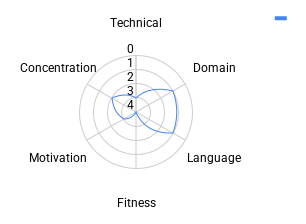
\includegraphics[width=0.85\textwidth]{images/david_chart.png}
    \end{center}

    \vspace{0.2cm}

    \begin{center}
    \renewcommand{\arraystretch}{1.3}
    \begin{tabular}{|l|c|c|}
        \hline
        \textbf{Dimension} & \textbf{Score (1--5)} & \textbf{Indicator} \\
        \hline
        Technical competence &
        \textbf{4} &
        \cellcolor{gray!10} \makebox[50pt]{\rule{10pt}{10pt}\rule{10pt}{10pt}\rule{10pt}{10pt}\rule{10pt}{10pt}\color{lightgray}\rule{10pt}{10pt}} \\
        \hline
        Domain competence &
        \textbf{2} &
        \cellcolor{gray!10} \makebox[50pt]{\rule{10pt}{10pt}\rule{10pt}{10pt}\color{lightgray}\rule{10pt}{10pt}\rule{10pt}{10pt}\rule{10pt}{10pt}} \\
        \hline
        Language competence &
        \textbf{2} &
        \cellcolor{gray!10} \makebox[50pt]{\rule{10pt}{10pt}\rule{10pt}{10pt}\color{lightgray}\rule{10pt}{10pt}\rule{10pt}{10pt}\rule{10pt}{10pt}} \\
        \hline
        Physical and visual ability &
        \textbf{5} &
        \cellcolor{gray!10} \makebox[50pt]{\rule{10pt}{10pt}\rule{10pt}{10pt}\rule{10pt}{10pt}\rule{10pt}{10pt}\rule{10pt}{10pt}} \\
        \hline
        Motivation &
        \textbf{4} &
        \cellcolor{gray!10} \makebox[50pt]{\rule{10pt}{10pt}\rule{10pt}{10pt}\rule{10pt}{10pt}\rule{10pt}{10pt}\color{lightgray}\rule{10pt}{10pt}} \\
        \hline
        Concentration &
        \textbf{3} &
        \cellcolor{gray!10} \makebox[50pt]{\rule{10pt}{10pt}\rule{10pt}{10pt}\rule{10pt}{10pt}\color{lightgray}\rule{10pt}{10pt}\rule{10pt}{10pt}} \\
        \hline
    \end{tabular}
    \end{center}

    \vspace{0.2cm}
    {\small \textbf{Legend:} \rule{10pt}{10pt} = achieved value \hfill \color{lightgray}\rule{10pt}{10pt}\color{black} = not achieved value}
\end{tcolorbox}

% ================================================================
% USE CASE #1: «The renewal that cannot be seen»
% ================================================================

\begin{tcolorbox}[sectionbox,colback=primaryColor!10]
    \textbf{Use Case description \#1: Online subscription renewal completed successfully but fined on board --- the unexplained post-purchase}
\end{tcolorbox}

\vspace{0.3cm}

% --- Narrative ---
\begin{tcolorbox}[base]
    {\small
    \textbf{Scenario:} User (technical competence 4/5, language competence 2/5, domain competence 2/5) already has an account on \texttt{solweb.tper.it} created with assistance. Attempts renewal independently.

    \textbf{Objective:} Renew TPER monthly subscription and use it correctly on board.

    \textbf{Sequence:}
    \begin{enumerate}
        \item The user opens \texttt{solweb.tper.it}, logs in (familiar procedure), navigates to ``Monthly subscription renewal'' and completes payment with credit card. Time: 5 minutes. Linear operation.
        \item The system shows ``Payment successful'' and sends an email with PDF receipt. No additional message on how to make the ticket valid on board. The user saves the receipt on his phone.
        \item The next day, the user gets on the bus. At the check, he shows the PDF receipt. The inspector refuses: ``The subscription must be loaded on Mi Muovo or the TPER app. This is only the receipt.''
        \item The inspector issues a fine of 60\euro{} for travel without a valid ticket. The user paid 50\euro{} for the subscription and receives a 60\euro{} fine.
        \item Post-event: the user consults an Italian colleague and discovers the activation procedure never communicated during checkout. The purchase flow never mentioned the loading step.
    \end{enumerate}

    \textbf{Barriers:}
    \begin{itemize}
        \item \textbf{RF-18} --- The checkout ends with payment confirmation without instructing on how to make the subscription valid on board.
        \item \textbf{RF-19} --- Ecosystem fragmentation (solweb = purchase, Mi Muovo = physical medium, TPER app = digital) never made explicit to the user.
        \item \textbf{RF-20} --- No message during purchase about post-payment steps.
    \end{itemize}

    \textbf{Outcome:} Purchase completed (transactional success). Use failed (experiential failure). Economic damage: 60\euro{} fine + 50\euro{} subscription = 110\euro{} total for a 50\euro{} service.

    \textbf{Times:} 15 minutes purchase + 10 minutes check + 15 minutes intermediary explanation.
    }
\end{tcolorbox}

\vspace{0.3cm}

% ================================================================
% USE CASE #2: "The hidden discount"
% ================================================================

\begin{tcolorbox}[sectionbox,colback=primaryColor!10]
    \textbf{Use Case description \#2: Search for fare discounts --- opaque information and absent language hide real savings}
\end{tcolorbox}

\vspace{0.3cm}

\begin{tcolorbox}[base]
    {\small
    \textbf{Scenario:} User (language competence 2/5, domain competence 2/5) pays full-price subscription (50\euro{}/month) for 3 months. A colleague informs him of discounted fares for ISEE under 16,000\euro{}. The user is unfamiliar with ISEE, Carta Agevolata, DSU.

    \textbf{Objective:} Find out if he is entitled to discounts or concessions on the TPER monthly subscription.

    \textbf{Sequence:}
    \begin{enumerate}
        \item The user searches ``discount'' in the \texttt{tper.it} search bar: 0 results. Tries ``sconti'': 0. Tries ``agevolazioni'': pages with titles ``Carta Agevolata'', ``ISEE'', ``DSU'' --- untranslated terms lacking context for a foreign user.
        \item The user navigates the menu: ``Subscriptions'' $\rightarrow$ ``Discounts''. Page with dense Italian bureaucratic text: requirements, thresholds, resolutions. No language selector present.
        \item The user tries Google Translate: the acronyms (ISEE, DSU) remain unchanged. ``Carta Agevolata'' translated literally, without explanation of meaning.
        \item After 15 minutes of attempts, the user gives up. The next day he asks his colleague, who verifies: the user is entitled to a discounted fare (30\euro{} instead of 50\euro{}).
    \end{enumerate}

    \textbf{Barriers:}
    \begin{itemize}
        \item \textbf{RF-21} --- Internal search does not support synonyms or intents (``discount'' $\neq$ ``agevolazioni'').
        \item \textbf{RF-22} --- Bureaucratic terms (ISEE, DSU) not explained: no tooltip/glossary.
        \item \textbf{RF-23} --- Informative pages not available in English. Google Translate ineffective on acronyms.
    \end{itemize}

    \textbf{Outcome:} Information not discovered independently. The user suffers an economic loss of 60\euro{} over 3 months (150\euro{} paid vs. 90\euro{} due), attributable to the site's informational opacity.

    \textbf{Cost of opacity:} 60\euro{} over 3 months (20\euro{}/month extra cost).
    }
\end{tcolorbox}

\vspace{0.3cm}

% ================================================================
% IMPACT OF PERSONA AND USE CASES ON DESIGN
% ================================================================

\begin{tcolorbox}[sectionbox,colback=primaryColor!10]
    \textbf{Concluding considerations --- Impact of persona and use cases on design}
\end{tcolorbox}
\vspace{0.3cm}

\begin{tcolorbox}[base]
    {\small
    \textbf{Impact of persona David Carter on design:} \\[4pt]
    Profile: technical competence 4/5, domain competence 2/5, language competence 2/5. Requirements emerged:

    \begin{itemize}[leftmargin=*]
        \item \textbf{RF-24 --- Contextual glossary for domain terminology (cfr. D3):} Terms like ``Mi Muovo'', ``Codice Fiscale'', ``ISEE'', ``DSU'', ``Carta Agevolata'' must be accompanied by explanatory tooltips and, for non-Italian users, by contextual translations. For language competence 2/5, unexplained terms block the flow.

        \item \textbf{RF-25 --- Multilingual support in registration and purchase flows (cfr. R12):} The English interface on \texttt{solweb.tper.it} must be available \textit{before} login, not after. The foreign user needs the foreign language precisely during registration and first access.

        \item \textbf{RF-26 --- Intent-based search engine (cfr. R2):} Internal search must support synonyms and semantic queries (``discount'', ``sconti'', ``monthly pass'') beyond exact bureaucratic terminology. For a user unfamiliar with the domain, formulating the right query must not be a prerequisite.

        \item \textbf{RF-27 --- Informative content in clear language (cfr. D2, R3):} Descriptive pages (subscriptions, discounts) must use a non-bureaucratic tone, explaining regulatory concepts (ISEE, DSU, resolutions) in language accessible even to those unfamiliar with the Italian institutional context.
    \end{itemize}
    }
\end{tcolorbox}

\vspace{0.3cm}

\begin{tcolorbox}[base]
    {\small
    \textbf{Impact of Use Case \#1 (The renewal you don't see) on design:} \\[4pt]
    \begin{itemize}[leftmargin=*]
        \item \textbf{RF-28 --- Mandatory post-purchase procedural guide (cfr. R10):} The checkout flow must not end at payment. It must include an ``Instructions for use'' screen explaining how to make the subscription valid on board (loading on Mi Muovo/TPER app). The email receipt must be accompanied by clear procedural instructions.

        \item \textbf{RF-29 --- Explicit mapping of the multi-platform ecosystem (cfr. D5, R4):} The system must explicitly declare the relationships between platforms (solweb = purchase, Mi Muovo = physical medium, TPER app = digital) at the right time, not after the fact. The user must know which platform they are operating on and what happens next.

        \item \textbf{Cost of missing guidance:} A fine of 60\euro{} for a subscription paid 50\euro{} (damage >100\% of the transaction value) is an unacceptable economic consequence generated exclusively by the system's procedural opacity.
    \end{itemize}
    \vspace{0.2cm}
    \textbf{Impact of Use Case \#2 (The hidden discount) on design:} \\[4pt]
    \begin{itemize}[leftmargin=*]
        \item \textbf{RF-30 --- Semantic and intent-based search (cfr. R2):} The internal search engine must return results for ``discount'', ``sconti'', ``risparmio'' as well as ``agevolazioni''. For a user with language competence 2/5 and domain competence 2/5, knowing the exact bureaucratic term cannot be a prerequisite.

        \item \textbf{RF-31 --- Information equity: terminology explained (cfr. D3):} Bureaucratic terms (ISEE, DSU) must be accompanied by explanations in simple language, tooltips, and translations. Terminological opacity selectively affects the users who most need discounts, constituting a problem of equity as well as usability.

        \item \textbf{RF-32 --- Informative pages in English (cfr. R12):} Pages on fares and discounts must be available in English. Google Translate does not translate bureaucratic acronyms, making discount information effectively invisible for non-Italian speakers.
    \end{itemize}
    }
\end{tcolorbox}
\begin{center}
    {\color{primaryColor}\Large\bfseries Persona and Use Case Card} \\[4pt]
    {\color{secondaryColor}\normalsize Phase B --- Feasibility Study} \\[4pt]
    {\color{secondaryColor}\small This \textit{persona} is \textbf{not} the protagonist (i.e., is not the person for whom we are designing the new tool; is a supporting cast member who must nevertheless be taken into account to ensure an inclusive design).}
\end{center}

\vspace{0.3cm}
{\color{borderColor}\hrule}
\vspace{0.4cm}

\begin{minipage}[t]{0.25\textwidth}
    \centering
    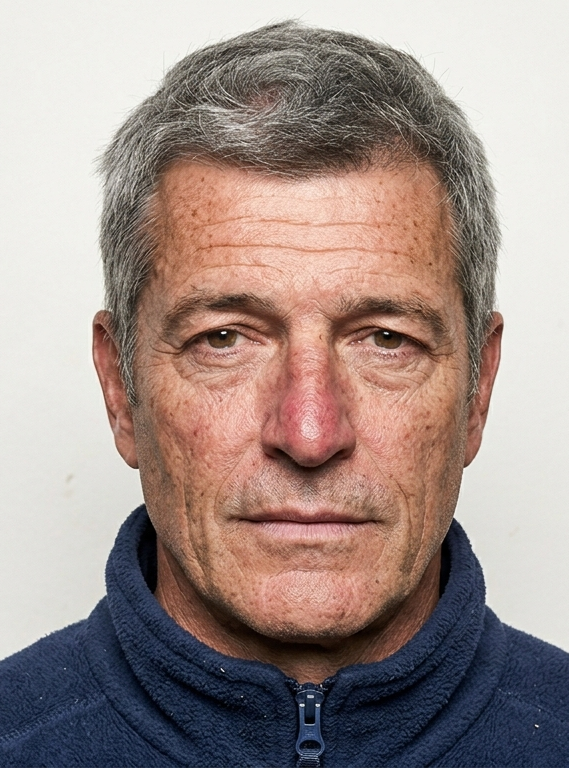
\includegraphics[width=\textwidth,height=5cm,keepaspectratio]
    {images/roberto.png}
    \vspace{0.2cm}
\end{minipage}
\hfill
\begin{minipage}[t]{0.70\textwidth}
    \begin{tcolorbox}[personabox]
        \textbf{\large Roberto Rinaldi}\label{persona:roberto_rinaldi} \\[4pt]
        {\color{secondaryColor}\small\textbf{Meaningful quote:}
        \textit{``Honestly, sitting down at the computer to read pages and pages of instructions makes me lose interest. I prefer going to the counter so the operator does everything, even though it embarrasses me a bit to have to ask a thousand questions if there's a long queue.''}} \\[4pt]
        {\color{secondaryColor}\small\textbf{Corresponding segment:}
        \hyperref[seg:cittadino]{[S3]} The citizen at the counter (Italian, 36--64 years old, low digital competence, institutional and occasional relationship with TPER, strong need for physical assistance).}
    \end{tcolorbox}
\end{minipage}

\vspace{0.3cm}

% ================================================================
% PERSONA DESCRIPTION (Basic Facts)
% ================================================================

\begin{tcolorbox}[base]
    \textbf{Persona description} \\[4pt]
    {\small
    \textbf{Age:} 54 \hfill
    \textbf{Gender:} Male \hfill
    \textbf{Nationality:} Italian
    \\[2pt]
    \textbf{Residence:} Bologna, suburban district (Borgo Panigale) \hfill
    \textbf{Marital status:} Separated \\[2pt]
    \textbf{Profession and Income:} School aide (ATA staff) with a fixed-term contract. He has a low ISEE due to the recent period of unemployment and the rent he pays for a small shared room. \\[2pt]
    \textbf{Language proficiency:} Native Italian speaker. He understands the language perfectly, but gets bored immediately in front of bureaucratic language and dense walls of text typical of institutional sites, preferring to avoid the effort of reading and interpreting them. \\[2pt]
    \textbf{Relevant physical issues:} No serious motor problems; suffers from mild presbiopia (uses reading glasses for close vision) and some back aches caused by manual labor performed in the past. \\[2pt]
    \textbf{Digital profile:} He owns a low-end smartphone that he uses to make calls, send WhatsApp messages to his children, and watch a few videos or news. He does not suffer from technophobia or computer security anxiety, but is extremely lazy in digital learning: if a procedure requires more than two steps or mental application on structured forms, he gets bored and abandons. He has not activated SPID simply because he kept postponing the process, finding it a boring waste of time. \\[2pt]
    \textbf{TPL usage:} Until three months ago, he only used the car. Arriving in Bologna, he found himself without a car and must rely entirely on buses to go to school. He currently pays for single or daily tickets, wasting a lot of money, and does not yet have a subscription. He constantly postpones the purchase out of pure inertia, still not knowing well the lines or fare rules of the service.
    }
\end{tcolorbox}

\vspace{0.3cm}

% ================================================================
% BACKGROUND AND PSYCHOLOGICAL CHARACTERISTICS
% ================================================================

\begin{tcolorbox}[base]
    \textbf{Background and psychological characteristics} \\[4pt]
    {\small
    Roberto worked for thirty years as a factory worker in a small artisan company on the Emilian Apennines, in a town where everyone knew each other and people only moved by car. Due to the company's closure, he went through a period of unemployment. Three months ago he finally obtained a yearly assignment as a school aide and moved to Bologna alone. His children work in other regions and he tends not to bother them for daily bureaucratic matters he considers boring. \\[4pt]

    \textbf{Poor Domain Knowledge and Inertia:} Bologna for Roberto is still a new and dispersive reality. He is not used to the thousand bus lines and the concept of ``fare zones''. Having poor knowledge of the transportation domain, he prefers not to make the effort to study it online, showing strong apathy and a passive attitude toward TPER rules. \\[4pt]

    \textbf{Laziness and Lack of Motivation/Concentration:} His reduced attention does not stem from fear of making mistakes or concerns about data security, but from a deep mental laziness toward digital bureaucracy. In front of an information screen or an online form, Roberto immediately loses concentration; he reads in jumps, gets distracted easily, and decides it is more convenient to have someone else handle the matter. His strategy to save time and cognitive energy is to delegate the entire effort directly to the physical counter operator. \\[4pt]

    \textbf{Shyness in Uncomfortable Situations:} Despite the preference for the physical channel, Roberto is a shy and introverted man who fears the judgment of others. When he shows up at the counter, the idea of having to ask too many questions or slow down the people in line makes him uncomfortable. In these awkward situations he reveals himself as somewhat clumsy: he pulls crumpled papers from his pockets in a confused manner, often apologizes to the clerk, and, if he feels the pressure of the line behind him, tends to hurry up, passively accepting the instructions without delving into his real doubts.
    }
\end{tcolorbox}

\vspace{0.3cm}

% ================================================================
% C&A DIAGRAM
% ================================================================

\begin{tcolorbox}[personabox]
    \textbf{Competences and Abilities Chart (C\&A Diagram)} \\[4pt]
    {\small
    }

     \begin{center}
    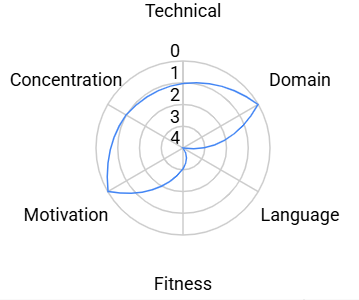
\includegraphics[width=0.85\textwidth]{images/robertochart.png}
    \end{center}

    \vspace{0.3cm}

    \begin{center}
    \renewcommand{\arraystretch}{1.3}
    \begin{tabular}{|l|c|c|}
        \hline
        \textbf{Dimension} & \textbf{Score (1--5)} & \textbf{Indicator} \\
        \hline
        Technical competence &
        \textbf{2} &
        \cellcolor{gray!10} \makebox[50pt]{\rule{10pt}{10pt}\rule{10pt}{10pt}\color{lightgray}\rule{10pt}{10pt}\rule{10pt}{10pt}\rule{10pt}{10pt}} \\
        \hline
        Domain competence &
        \textbf{1} &
        \cellcolor{gray!10} \makebox[50pt]{\rule{10pt}{10pt}\color{lightgray}\rule{10pt}{10pt}\rule{10pt}{10pt}\rule{10pt}{10pt}\rule{10pt}{10pt}} \\
        \hline
        Language competence &
        \textbf{5} &
        \cellcolor{gray!10} \makebox[50pt]{\rule{10pt}{10pt}\rule{10pt}{10pt}\rule{10pt}{10pt}\rule{10pt}{10pt}\rule{10pt}{10pt}} \\
        \hline
        Physical and visual ability &
        \textbf{4} &
        \cellcolor{gray!10} \makebox[50pt]{\rule{10pt}{10pt}\rule{10pt}{10pt}\rule{10pt}{10pt}\rule{10pt}{10pt}\color{lightgray}\rule{10pt}{10pt}} \\
        \hline
        Motivation &
        \textbf{1} &
        \cellcolor{gray!10} \makebox[50pt]{\rule{10pt}{10pt}\color{lightgray}\rule{10pt}{10pt}\rule{10pt}{10pt}\rule{10pt}{10pt}\rule{10pt}{10pt}} \\
        \hline
        Concentration &
        \textbf{2} &
        \cellcolor{gray!10} \makebox[50pt]{\rule{10pt}{10pt}\rule{10pt}{10pt}\color{lightgray}\rule{10pt}{10pt}\rule{10pt}{10pt}\rule{10pt}{10pt}} \\
        \hline
    \end{tabular}
    \end{center}

    \vspace{0.2cm}
    {\small \textbf{Legend:} \rule{10pt}{10pt} = achieved value \hfill \color{lightgray}\rule{10pt}{10pt}\color{black} = not achieved value}

\end{tcolorbox}

\vspace{0.3cm}

% ================================================================
% ADDITIONAL INTERESTING DETAILS
% ================================================================

\begin{tcolorbox}[base,colback=backgroundColor!50]
    \textbf{Additional interesting details} \\[4pt]
    {\small
    \begin{itemize}[leftmargin=*]
        \item When out of inertia he tries to open the web portal, he stops at the homepage: the absence of an ultra-fast path or immediate indications prompts him to close the tab after a few seconds, dismissing the reading with a lazy \textit{``I'll think about it another day''}.
        \item Knowing he has a low ISEE but having no desire to decipher the requirements online, he blindly trusts the word-of-mouth of a colleague who told him to go in person and ask for \textit{``the subscription with ISEE discounts''}. He wrote down this exact phrase on a piece of paper to avoid getting confused or freezing up in front of the clerk due to his shyness.
        \item He represents the classic example of a user who risks showing up physically at the counter without the correct documents (such as the DSU or the valid official ISEE certificate, bringing instead useless paperwork), not because of a digital divide or anxiety problem, but because he performed a superficial and half-hearted preventive check on the public website.
    \end{itemize}
    }
\end{tcolorbox}

% ================================================================
% USE CASE #1: ROBERTO RINALDI
% ================================================================
\begin{tcolorbox}[sectionbox,colback=primaryColor!10]
    \textbf{Use Case description \#1: Attempted discounted subscription request between physical counter and online channel}
\end{tcolorbox}

\vspace{0.3cm}

% --- Use Case Narrative ---
\begin{tcolorbox}[base]
    {\small
    \textbf{Scenario:} User (motivation 1/5, concentration 2/5, technical competence 3/5) attempts to request a discounted subscription. First approach: physical channel (counter). Failure due to missing documentation. Second approach: digital channel (website). Abandonment due to informational complexity.

    \textbf{Objective:} Discover required documents for discounted subscription and start the procedure.

    \textbf{Sequence:}
    \begin{enumerate}
        \item \textbf{Physical:} The user goes to the ticket office (40 minutes waiting). The operator requests current ISEE certification + passport photo. The user only has plastic fiscal code card and pay slip. Operation failed.
        \item \textbf{Counter abandonment:} Social pressure of the queue. The user leaves without asking for information (no reminder, QR code, or instruction received).
        \item \textbf{Digital:} The user searches ``TPER discount subscription'' on Google, lands on the fare discounts page \texttt{tper.it}. Bureaucratic register (ISEE, DSU, brackets, resolutions) exceeds the attention threshold.
        \item \textbf{Site abandonment:} Scrolls quickly, does not find an answer to ``what do I need?''. Closes the tab in $<$2 minutes.
        \item \textbf{Consequence:} Procrastinates indefinitely. Continues to pay full-price rides. The economic need (low ISEE) does not translate into action.
    \end{enumerate}

    \textbf{Barriers:}
    \begin{itemize}
        \item \textbf{RF-33} --- No omnichannel continuity: at the counter, the operator does not provide paper/digital support for resuming from home.
        \item \textbf{RF-34} --- Discount pages in bureaucratic language: incompatible with concentration 2/5.
        \item \textbf{RF-35} --- No preventive pre-counter checklist: the user arrives without the correct documents.
    \end{itemize}

    \textbf{Outcome:} Double failure (physical due to documents, digital due to complexity). The system loses a potential subscriber with real economic need.

    \textbf{Times:} 40 minutes (queue) + 5 minutes (counter) + $<$2 minutes (browsing) = 47 minutes, no result.
    }
\end{tcolorbox}

% ================================================================
% CONCLUDING CONSIDERATIONS --- IMPACT ON DESIGN
% ================================================================
% ================================================================
% CONCLUDING CONSIDERATIONS --- IMPACT ON DESIGN (FOCUS ISTITUZIONALE)
% ================================================================
\begin{tcolorbox}[sectionbox,colback=primaryColor!10]
    \textbf{Concluding considerations --- Impact of persona on design in the institutional context}
\end{tcolorbox}

\vspace{0.3cm}

\begin{tcolorbox}[base]
    {\small
    \textbf{Impact of persona Roberto Rinaldi on design:} \\[4pt]
    Roberto is the only persona in the cast who has no language barriers nor technological anxiety (technical competence 3/5, language competence 5/5), yet he fails. His profile demonstrates that the obstacle is the gap between the effort required by the system and the effort the user is willing to invest (motivation 1/5, concentration 2/5).

    \begin{itemize}[leftmargin=*]
        \item \textbf{RF-36 --- ``Am I entitled to a discount?'' path in $\leq$3 clicks:} With motivation 1/5, the user does not explore dense pages. A guided path is needed that in 2--3 steps tells the user which documents are needed and how to obtain them, without assuming familiarity with bureaucratic terminology.

        \item \textbf{RF-37 --- Non-bureaucratic communication register:} The discount pages use resolutions, brackets, acronyms (ISEE, DSU). For a user with concentration 2/5, even as a native Italian speaker, this register constitutes a barrier. The mother tongue is not enough if the register is wrong.

        \item \textbf{RF-38 --- Content for skim-reading, not for in-depth reading:} The user reads in jumps, scrolls quickly, looks for immediate solutions. Endless pages and downloadable PDFs are the worst format for this profile. The system must offer synthetic content with visible call-to-action without scrolling.

        \item \textbf{RF-39 --- Post-recovery support at the counter:} The social pressure of the queue and the embarrassment of missing documents drive the user away from the physical channel. The system must provide a recovery mechanism (e.g. operator hands over a sheet/QR code with instructions to complete the procedure online) that intercepts the user before they definitively abandon.
    \end{itemize}
    }
\end{tcolorbox}

\vspace{0.3cm}

\begin{tcolorbox}[base]
    {\small
    \textbf{Impact of Use Case \#1 on design:} \\[4pt]
    The double failure (physical channel due to embarrassment, digital channel due to complexity) shows that the system loses users on both channels for different but convergent reasons.

    \begin{itemize}[leftmargin=*]
        \item \textbf{RF-40 --- Proactive physical-digital bridge:} When leaving the counter without a completed procedure, the user must receive a support (sheet/QR code) with instructions on how to resume from home. The two channels must not be treated as separate worlds.

        \item \textbf{RF-41 --- Informative content in citizen-friendly, not bureaucratic, language:} The discount pages must explain ISEE, DSU, brackets in language accessible to those who have just discovered they are entitled to a discount. No technical term without contextual explanation.

        \item \textbf{RF-42 --- Quick path ``Am I entitled to a discount?'' on the homepage:} The homepage must offer a visible quick path that in $\leq$2 steps tells the user which documents are needed. For motivation 1/5, the absence of a shortcut is equivalent to the absence of the service.

        \item \textbf{RF-43 --- Preventive visual pre-counter checklist:} Before going to the counter, the user must be able to consult a visual list of the required documents. 40 minutes of queue + embarrassment + escape are preventable with an upstream check.
    \end{itemize}
    }
\end{tcolorbox}


\newpage
\section{Cast Card}

\subsection{Cast with roles and segments}

\begin{tcolorbox}[base]
\begin{center}
{\small
\renewcommand{\arraystretch}{1.3}
\resizebox{\textwidth}{!}{%
\begin{tabular}{|p{2.3cm}|p{1.8cm}|p{2.7cm}|p{6.5cm}|}
\hline
\textbf{Persona} & \textbf{Role} & \textbf{Segment} & \textbf{Profile summary} \\
\hline
Fatima Benali & \textbf{Protagonist} & Variant S1/S2 & 68 years, Moroccan,
literate in Arabic, illiterate in written Italian, minimal digital
competence, learning through visual imitation \\
\hline
Liliana Roversi & Non-protagonist & \hyperref[seg:anziana]{[S1]} The elderly
commuter & 79 years, Italian, minimal digital competence, lives alone, strong
frustration with digital dependency \\
\hline
David Carter & Non-protagonist & \hyperref[seg:straniero]{[S2]} The foreign
worker & 32 years, British, high technical competence, language and systemic
barrier, seconded to Bologna for 12 months \\
\hline
Roberto Rinaldi & Non-protagonist & \hyperref[seg:cittadino]{[S3]} The citizen
at the counter & 54 years, Italian, low motivation for digital
learning, shyness at the counter, low ISEE \\
\hline
\end{tabular}%
}
}
\end{center}
\end{tcolorbox}

\vspace{0.5cm}

\subsection{Cumulative Chart of Personality Traits}

\begin{figure}[H]
\centering
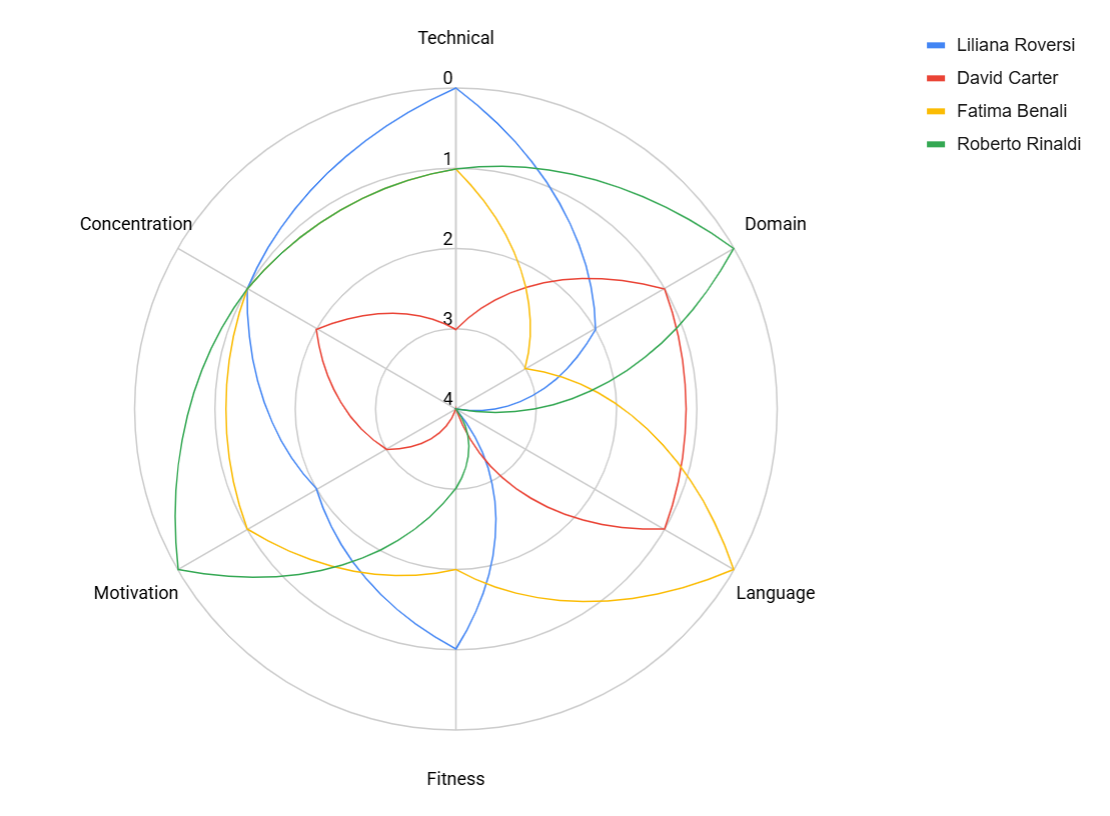
\includegraphics[width=0.95\textwidth]{images/cumulativechart.png}
\caption{Cumulative comparison of personality traits among the four personas.
The chart shows how the profiles are complementary: no persona excels
in all dimensions, and each one's weaknesses correspond to the
strengths of another.}
\label{fig:cumulative-chart}
\end{figure}

\vspace{0.5cm}

\subsection{Impact on Design --- Requirements emerging from Personas}

\begin{tcolorbox}[base]
{\small
\renewcommand{\arraystretch}{1.3}
\begin{tabular}{|p{1.2cm}|p{5cm}|p{5cm}|p{2.8cm}|}
\hline
\textbf{Code} & \textbf{Problem} & \textbf{Solution} & \textbf{Personas} \\
\hline
\textbf{PR-01} & The interface is entirely textual in the Latin
alphabet. Forms ask for data from physical documents without showing where
to find them. Anyone who cannot read text or recognize documents by shape and
color is excluded. & Use universal icons, photographs, color codes.
For each requested data field, show a visual reproduction of the physical
document with the data highlighted. & Fatima (primary), Liliana, Roberto \\
\hline
\textbf{PR-02} & The system assumes learning through reading and
textual decoding, incompatible with those who learn through visual
imitation and repetition (``watch and repeat''). & Flows must be
learnable by observation, not by reading. Provide visual
demonstrations and the ability to repeat steps. & Fatima,
Liliana \\
\hline
\textbf{PR-03} & Every non-essential step before the task (e.g.
registration) consumes attention that will not be recoverable. Fragile
personas have an average concentration of 2/5. & Eliminate unnecessary steps
before the target operation. Offer paths with the fewest
possible steps. & Fatima, Liliana, Roberto \\
\hline
\textbf{PR-04} & Labels and content use bureaucratic terminology
(Mi Muovo, ISEE, DSU, Boost) without explanation. Even native Italian
speakers give up when faced with pages written for insiders. &
Provide inline explanations for every technical term. Write
content in plain language, with progressive disclosure from
summary to detail. & David, Roberto, Fatima \\
\hline
\textbf{PR-05} & The internal search requires the exact terminology of the
domain (``agevolazioni'') and does not support synonyms or queries in other
languages (``sconti'', ``discount''). & Implement a search engine
with support for synonyms, multilingual queries and contextual
suggestions based on real intents. & David, Roberto \\
\hline
\end{tabular}}
\end{tcolorbox}

\vspace{0.5cm}

\subsection{Impact on Design --- Requirements emerging from Use Cases}

\begin{tcolorbox}[base]
{\small
\renewcommand{\arraystretch}{1.3}
\begin{tabular}{|p{1.2cm}|p{5cm}|p{5cm}|p{2.8cm}|}
\hline
\textbf{Code} & \textbf{Problem} & \textbf{Solution} & \textbf{Personas} \\
\hline
\textbf{UR-01} & The transition from \texttt{tper.it} to
\texttt{solweb.tper.it} happens without warning. The user does not know they have
changed platforms nor why the interface is different. For those who
orient themselves by shapes and colors, it feels like landing on another site. &
Explicitly signal the transition with a notice explaining: ``To
complete the operation we are taking you to the purchase
platform. The look changes but you are still on TPER.'' & Fatima, Liliana \\
\hline
\textbf{UR-02} & After payment, the system does not explain what to do with
the purchased ticket. The PDF receipt is not a valid travel ticket,
but the user finds out only when fined on board. & Show a
post-purchase screen with visual step-by-step instructions: where to find
the ticket, how to load it onto the card, how to show it to the inspector.
& David \\
\hline
\textbf{UR-03} & For those who cannot read the interface language, an
error message is not an indication of how to fix it --- it is
confirmation that they broke something. The emotional impact blocks recovery. &
Errors must use non-textual signals (icon, color,
animation) that communicate ``it is a hiccup, not a disaster''. The
error text should be accompanied by a concrete and visual action. &
Fatima \\
\hline
\textbf{UR-04} & When the user leaves the counter without having
completed the procedure, they receive nothing to resume from home. The two
channels (physical and web) do not communicate, and the user who falls into the void between
them is lost. & Give the user a receipt with a QR
code that, scanned from home, takes them back to the incomplete procedure with the
data already entered by the operator and the list of missing documents. &
Roberto \\
\hline
\textbf{UR-05} & For a user with motivation 1/5, the absence of a
``Am I eligible for a discount?'' path is equivalent to the absence of the
service. The information pages require reading and interpreting
bureaucratic texts before discovering eligibility. & Offer an
interactive wizard with a few questions (age, ISEE, residence, frequency
of use) that in less than a minute tells the user which concessions
they are entitled to and which documents are needed. & Roberto, David \\
\hline
\end{tabular}}
\end{tcolorbox}

% ================================================================
% PHASE C: DESIGN PROPOSAL
% ================================================================
\newpage
\section{Phase C: Design Proposal}

Phase C translates recommendations R1--R13 into concrete design artifacts: Information Architecture, structural Blueprints, Wireframes, and a Before/After comparison of the proposed solution. The five deliverables produced are described below.

\vspace{0.3cm}

% ================================================================
\subsection{Information Architecture Card}


\begin{tcolorbox}[colback=primaryColor,colframe=primaryColor,arc=1.5mm,halign=center,valign=center,height=2cm]
 \color{white}\LARGE\bfseries\sffamily INFORMATION ARCHITECTURE CARD \\[0.1cm]
 \color{white!80}\small\sffamily Phase C --- Design Proposal
\end{tcolorbox}

\vspace{0.3cm}

% ===================================================================
% Q1: NECESSITY
% ===================================================================
\section{Need for an IA Phase}

\begin{tcolorbox}[rffield]
\small\textbf{Yes, necessary.} The TPER ecosystem has 6 channels (\texttt{tper.it} info, \texttt{solweb}, Roger, Punti Tper, tobacconists, contactless) with radically different functions, but the \texttt{tper.it} website --- the first point of contact for most users --- provides no structured guidance. Testing (Phase A) confirms that users do not know which channel to use for which purpose.
\end{tcolorbox}

% ===================================================================
% Q2: TOP-DOWN vs BOTTOM-UP
% ===================================================================
\section{Top-Down vs Bottom-Up Approach}

\begin{tcolorbox}[rffield]
\small
\textbf{Mixed approach ($\boxtimes$).}
\begin{itemize}[nosep]
  \item \textbf{Top-down}: From HPHP objectives --- \texttt{tper.it} exclusively informational, structured multi-channel guidance, IT/EN/AR support, route planner as a dedicated page.
  \item \textbf{Bottom-up}: From testing --- ``Where can I buy?'' is the most frequent question (UR-01), maximum depth of 2 clicks, non-corporate labels, separation of useful info / corporate news, suggested channel for each need (UR-02, UR-03), quick wizard to check eligibility for concessions (UR-05).
\end{itemize}
\end{tcolorbox}

% ===================================================================
% Q3: ORGANIZATION \& LABELING
% ===================================================================
\section{Organization and Labeling System}

\begin{tcolorbox}[rffield]
\small
\textbf{Organization by user intent} (currently: by corporate structure). \\

\noindent Menu: \texttt{[Home]} $\cdot$ \texttt{[Pianifica]} $\cdot$ \texttt{[Orari]} $\cdot$ \texttt{[Notizie]} $\cdot$ \texttt{[Dove Comprare]} $\cdot$ \texttt{[Biglietti]} $\cdot$ \texttt{[Abbonamenti]} $\cdot$ \texttt{[Aiuto]}. Depth: 1 click per section, no submenus. \\

\noindent\textbf{Labeling (vs existing):}
\begin{itemize}[nosep]
  \item ``Pianifica'' instead of ``Servizi di mobilit\`a''
  \item ``Dove Comprare'' instead of ``Reti di vendita'' (no ``Acquista'' that promises transactions)
  \item ``Abbonamenti'' instead of ``Mi Muovo''
\end{itemize}
\end{tcolorbox}

% ===================================================================
% Q4: METADATA
% ===================================================================
\section{Metadata Fields}

\begin{tcolorbox}[rffield]
\small
\renewcommand{\arraystretch}{1.1}
\begin{tabular}{|p{2.5cm}|p{5.5cm}|p{5cm}|}
\hline
\textbf{Category} & \textbf{Metadata} & \textbf{Difference} \\
\hline
Travel & \texttt{line, stop, zone, time} & Route planner + user search \\
\hline
Channels & \texttt{channel, operations, requirements, external\_link} & \textbf{New}: each content item associated with recommended channels \\
\hline
Titles & \texttt{type, price, purchase\_channels, documents} & \texttt{purchase\_channels} to guide the user \\
\hline
Guides & \texttt{channel, target, time, language, steps} & \textbf{New}: distinguishes user / intermediary \\
\hline
Language & \texttt{IT, EN, AR} & Structured multilingual support \\
\hline
\end{tabular}
\end{tcolorbox}

% ===================================================================
% Q5: NAVIGATION SYSTEM
% ===================================================================
\section{Navigation System}

\begin{tcolorbox}[rffield]
\small
\begin{enumerate}[nosep,leftmargin=*]
  \item \textbf{Horizontal menu by intent}: \texttt{[Home]} $\cdot$ \texttt{[Pianifica]} $\cdot$ \texttt{[Orari]} $\cdot$ \texttt{[Notizie]} $\cdot$ \texttt{[Dove Comprare]} $\cdot$ \texttt{[Biglietti]} $\cdot$ \texttt{[Abbonamenti]} $\cdot$ \texttt{[Aiuto]}
  \item \textbf{Informational hero}: ``Information channel'' badge + title + subtitle above the fold, followed by 6 quick navigation cards (Pianifica, Dove Comprare, Biglietti, Abbonamenti, Aiuto, Orari).
  \item \textbf{Channel guide banner}: On tickets, subscriptions, and homepage, an ``Are you looking to buy?'' box with direct links to solweb, Roger, and Punti Tper. Automatically activated after 3+ visits to informational pages without clicking on a purchase channel.
  \item \textbf{Channel comparison table}: In ``Dove Comprare'', all 5 channels compared by supported operations and available purchase channels. Replaces the ``Quick channels'' sidebar with an integrated, complete view.
  \item \textbf{Progress bar}: Step-by-step guides with progress indicator
  \item \textbf{Breadcrumb}: \texttt{Home > [Page]} on all main pages and \texttt{Login > Dashboard > Plans} in solweb flows.
  \item \textbf{News section in main menu}: Service news (diversions, strikes, timetables) accessible directly from the menu, filterable by category (Bologna, Ferrara, Bus, Railway, Diversions, Strikes, Parking). Link to institutional site in the footer.
  \item \textbf{Language switcher IT/EN/AR}: Persistent language selector in the header with dynamic translation and RTL support for Arabic.
  \item \textbf{Hamburger menu}: Collapsible menu on mobile with \texttt{aria-expanded} toggle.
  \item \textbf{Persistent info-banner}: ``tper.it is an informational website'' banner on every main page.
  \item \textbf{Channel redirect modal}: ``You are leaving tper.it'' notice when the user clicks links to external channels.
  \item \textbf{404 page}: Error page with return links to main sections.
\end{enumerate}
\end{tcolorbox}

% ===================================================================
% Q6: BROWSING AIDS
% ===================================================================
\section{Browsing Aids}

\begin{tcolorbox}[rffield]
\small
\begin{enumerate}[nosep,leftmargin=*]
  \item \textbf{Channel comparison table}: All 5 channels compared by supported operations with checkmark (\checkmark) and cross ($\times$)
  \item \textbf{Three interactive wizards}: 
    \begin{itemize}[nosep]
      \item \textbf{Dove Comprare}: 3 questions (service $\rightarrow$ channel $\rightarrow$ payment) $\rightarrow$ recommended channel with badge, icon, and link
      \item \textbf{Biglietti}: 5 questions $\rightarrow$ recommended ticket
      \item \textbf{Abbonamenti}: 6 questions $\rightarrow$ recommended subscription, includes the question ``Are you entitled to a concession?'' to check eligibility
    \end{itemize}
  \item \textbf{Visual icons per channel}: Each channel has a universal icon (monitor, smartphone, building, shop, card)
  \item \textbf{Position indicators}: Active menu item highlighted (\texttt{aria-current}), breadcrumb, color-coded cards by content type (6 colors)
  \item \textbf{Pill filters}: On Biglietti and Abbonamenti, filters by zone, duration, type, and concessions with result counter and reset
  \item \textbf{Accordion}: Expandable sections for FAQ (Aiuto) and purchase guides (Abbonamenti)
  \item \textbf{Back-to-top}: Fixed ``Back to top'' button appearing after 400px of scroll
  \item \textbf{Skeleton loading}: Animated placeholders during route planner results loading
  \item \textbf{Accessibility controls in header}: High contrast toggle, font scaling (A+/A-), skip-link to main content
  \item \textbf{Visual reproduction of physical documents}: In the document checklist, each document is accompanied by a visual mockup that highlights in yellow the data to find (e.g. ID card number, tax code, ISEE value). The user recognizes the document by shape and color without needing to read (PR-01).
  \item \textbf{Explanatory tooltips for technical terms}: On mouseover of bureaucratic terms (e.g. ISEE), a box appears with a plain language explanation and guidance on where to obtain the document (PR-04).
  \item \textbf{Non-textual error signals}: Fields with errors show a shake animation, \texttt{[!]} icon next to the input, and red border --- universal visual signals that communicate ``fix here'' without needing to read the message (UR-03).
\end{enumerate}
\end{tcolorbox}

% ===================================================================
% Q7: SEARCH AIDS
% ===================================================================
\section{Search Aids}

\begin{tcolorbox}[rffield]
\small
\begin{enumerate}[nosep,leftmargin=*]
  \item \textbf{Search bar always visible} in the header, expandable from magnifying glass icon. Modal overlay with placeholder: ``Search news, timetables, lines...''
  \item \textbf{Full-text search}: 11 indexed pages (Home, Pianifica, Orari, Notizie, Dove Comprare, Biglietti, Abbonamenti, Aiuto, Login, Sanzioni, Agevolazioni) with real-time results. Multilingual IT/EN/AR support with synonyms (e.g. ``sconto'' finds Biglietti and Abbonamenti, ``discount'' in English, in Arabic). Close via $\times$ button, click outside overlay, or Escape.

  \item \textbf{Autocomplete and contextual suggestions} (design, PR-05): Real-time suggestions as the user types, with automatic language detection and route, channel, or guide proposals based on real intents

\end{enumerate}
\end{tcolorbox}

% ===================================================================
% Q8: CONTENTS \& TASKS
% ===================================================================
\section{Contents and Tasks}

\begin{tcolorbox}[rffield]
\small
\textbf{5 priorities} (from user testing):

\begin{enumerate}[nosep,leftmargin=*]
  \item \textbf{Trip planning} (dedicated page): Route search with departure/destination, transport modes (bus/train/bike/walking), date/time, and simulated results
  \item \textbf{Purchase guide} (Dove Comprare): Comparison table + 3-question wizard (service $\rightarrow$ channel $\rightarrow$ payment) with recommended channel result
  \item \textbf{Abbonamenti}: Types, prices, documents, recommendation wizard, ``Are you entitled to a discount?'' wizard on dedicated page, pill filters, direct link to solweb
  \item \textbf{Biglietti}: Types, prices, zones, recommendation wizard, pill filters, purchase channels
  \item \textbf{Aiuto}: FAQ, step-by-step guides, trainer-mode activation, contacts
  \item \textbf{Solweb}: Complete purchase flow (login $\rightarrow$ dashboard $\rightarrow$ plans $\rightarrow$ documents $\rightarrow$ payment $\rightarrow$ confirmation) with guest variants (impersonal renewal, top-up, fines, card verification) and authenticated ones (purchase and personal renewal). Post-purchase instructions on conferma.html with 3 guided steps: receive the ticket, load it onto the card, show it to the inspector (UR-02).
\end{enumerate}

\noindent\textbf{Trainer-mode}: Activation FAB at the bottom right on all pages, with 5 modules (Rinnovo, Acquista, Pianifica, Biglietto, Ricarica), step-by-step walkthrough with visual highlights, session persistence, and printable summary at the end of each module.
\end{tcolorbox}

% ===================================================================
% Q9: INVISIBLE COMPONENTS
% ===================================================================
\section{Invisible Components}

\begin{tcolorbox}[rffield]
\small
\begin{itemize}[nosep]
  \item \textbf{Trainer session persistence} (\checkmark\ implemented): Saves current step, notes, language, verified documents via \texttt{localStorage}
  \item \textbf{QR code bridge Punto Tper $\rightarrow$ web} (design, UR-04): Receipt with QR code handed at the counter. Scanned from home, it returns to the incomplete procedure with data already pre-filled by the operator and the list of missing documents. Bridges the gap between physical and digital channels for procedures started but not completed
  \item \textbf{Persistent language preferences}: Cookie + browser detection, synchronized via QR
  \item \textbf{Anonymous analytics} (design): Channel visit tracking, guide completion rate
  \item \textbf{Printable summary} (\checkmark\ implemented): Generated in trainer-mode upon completion of each module, with print button and 14pt formatting
  \item \textbf{Multilingual preloading} (\checkmark\ implemented): \texttt{i18n.js} loads IT/EN/AR on startup
  \item \textbf{``Informational website'' disambiguation} (\checkmark\ implemented): ``Are you looking to buy?'' banner activated after 3+ visits to tickets/subscriptions/homepage pages without clicking on purchase channels
\end{itemize}
\end{tcolorbox}

\vspace{0.3cm}

% ================================================================

\newpage

\subsection{Structure Blueprint}

\begin{tcolorbox}[colback=primaryColor,colframe=primaryColor,arc=1.5mm,halign=center,valign=center,height=2cm]
 \color{white}\LARGE\bfseries\sffamily BLUEPRINT \\[0.1cm]
 \color{white!80}\small\sffamily Phase C --- Design Proposal
\end{tcolorbox}

\vspace{0.3cm}


The blueprints presented in this section define the components for content organization and the connections between them, following the course guidelines. Three distinct perspectives were created to represent different aspects of the TPER ecosystem:

\begin{itemize}
    \item \textbf{BP1} --- Information architecture of \texttt{tper.it} (structure perspective)
    \item \textbf{BP2} --- Multi-channel ecosystem (system perspective)
    \item \textbf{BP3} --- User journey from need to purchase (user perspective)
\end{itemize}

\noindent The blueprints were generated with HTML+CSS to ensure professional graphic rendering, then converted to PNG for inclusion in this document.

\vspace{0.3cm}

% =====================================================================
% BP1 --- INFORMATION ARCHITECTURE
% =====================================================================
\section{BP1 --- Information Architecture: tper.it}

\textit{Structure perspective.} This blueprint shows the hierarchical organization of content on \texttt{tper.it}, highlighting the clear separation between informational content (managed directly on the site) and purchase destinations (external channels). Orange arrows indicate redirects to the correct purchase channels.

\begin{figure}[H]
\centering
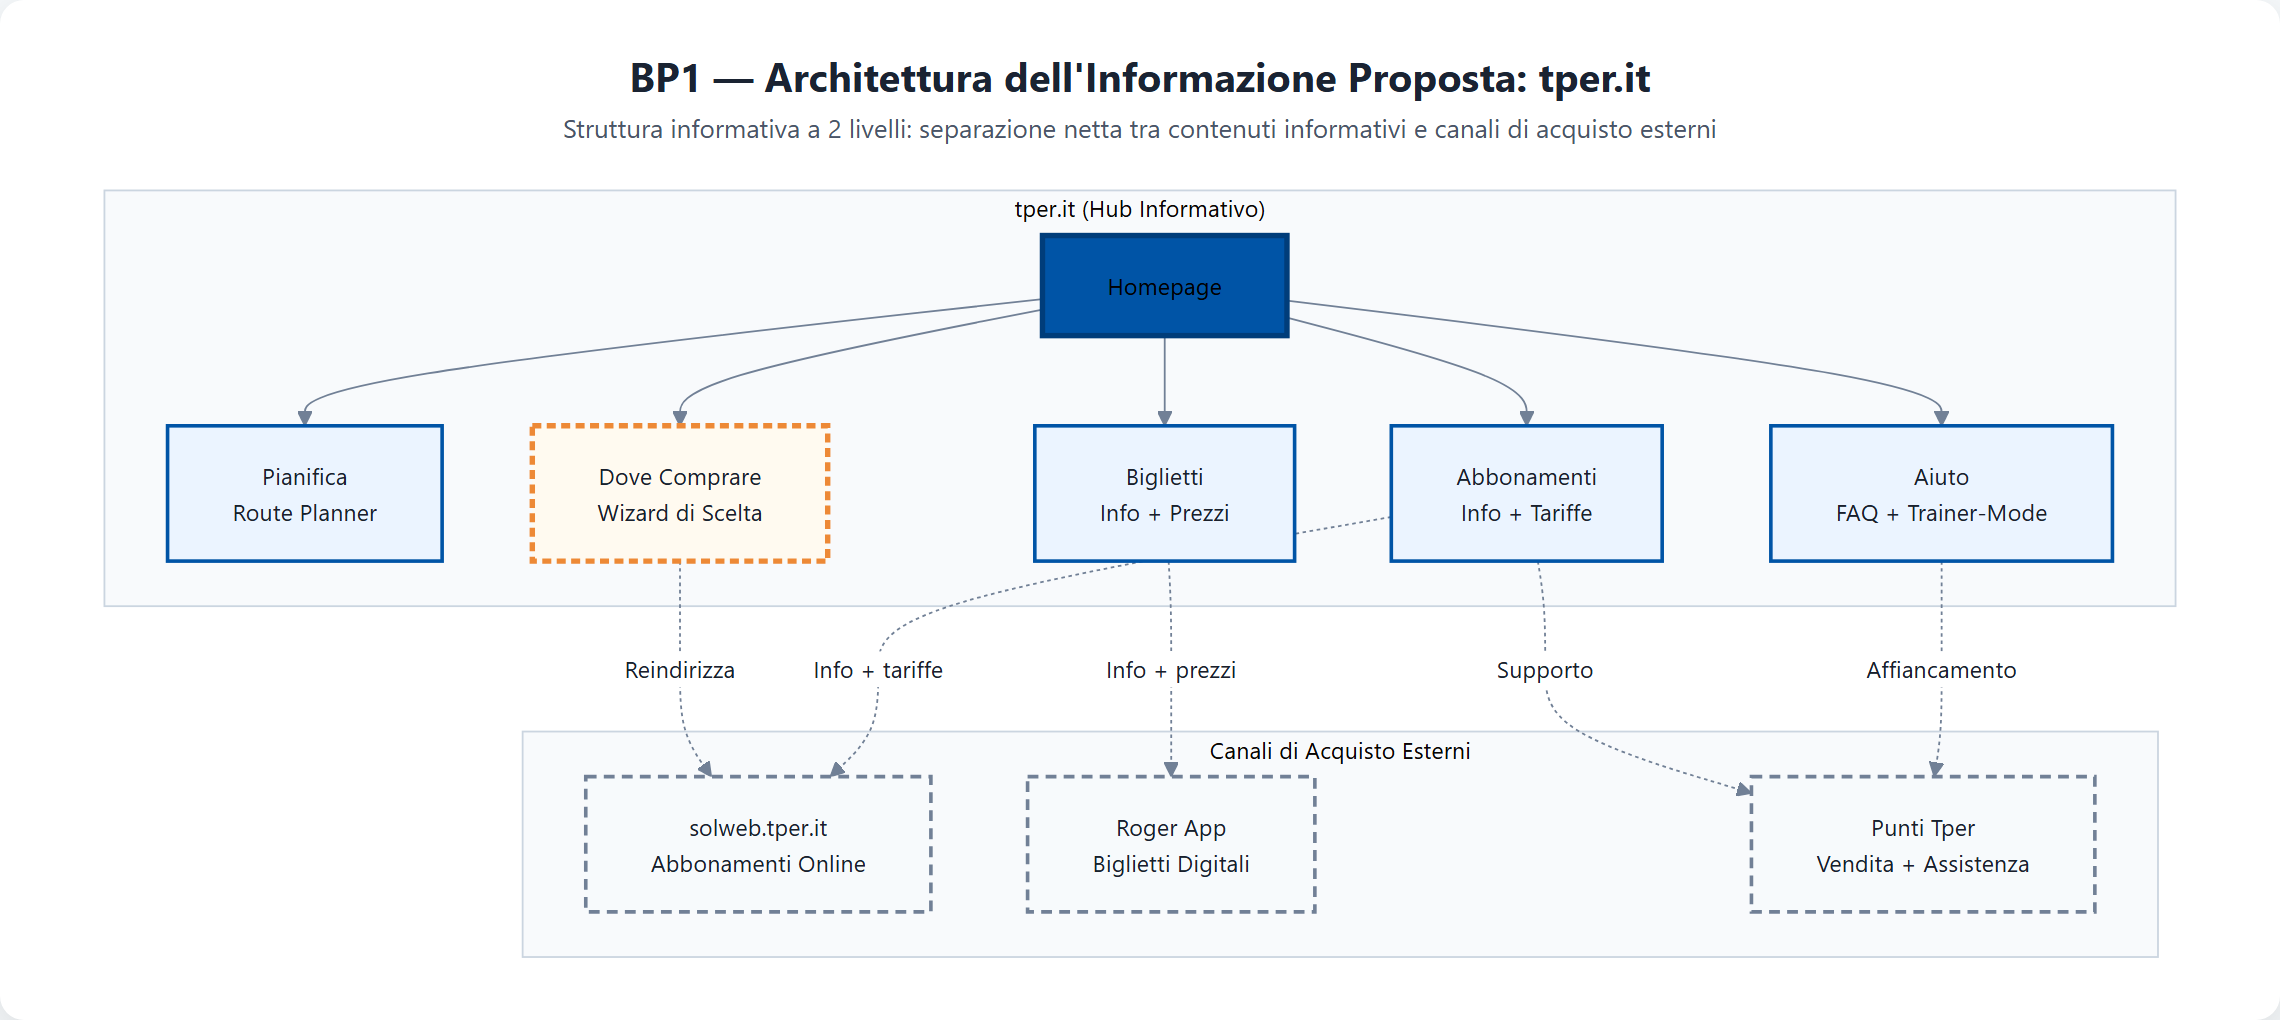
\includegraphics[width=\textwidth]{Blueprint/bp1-ia.png}
\caption{BP1 --- Information Architecture of \texttt{tper.it}}
\label{fig:bp1}
\end{figure}

\subsubsection*{Legend}
\begin{itemize}
    \item \textbf{Blue} --- Informational content managed on \texttt{tper.it}
    \item \textbf{Orange} --- Redirect to external channel for purchase
    \item \textbf{Purple/Green/Others} --- Purchase channels external to the \texttt{tper.it} ecosystem
\end{itemize}

\subsubsection*{Key Elements}
\begin{enumerate}
    \item \textbf{Route Planner as hero}: The primary function of \texttt{tper.it} is trip planning. The From--To search engine is prominently positioned on the homepage.
    \item \textbf{No purchases on tper.it}: Every section involving a financial transaction redirects the user to the appropriate channel (solweb, Roger, Punti Tper, tobacconists, contactless).
    \item \textbf{Clear separation}: Informational content (types, prices, guides) is managed on \texttt{tper.it}. Transactions take place exclusively on external channels.
    \item \textbf{Choice guide}: The ``Dove Comprare'' section acts as a decision hub that directs the user to the most suitable channel for their needs.
\end{enumerate}

\vspace{0.3cm}

% =====================================================================
% BP2 --- MULTI-CHANNEL ECOSYSTEM
% =====================================================================
\section{BP2 --- TPER Multi-Channel Ecosystem}

\textit{System perspective.} This blueprint illustrates the relationships between \texttt{tper.it} (informational channel) and the 5 purchase channels, showing the bridge mechanisms that connect information to transaction.

\begin{figure}[H]
\centering
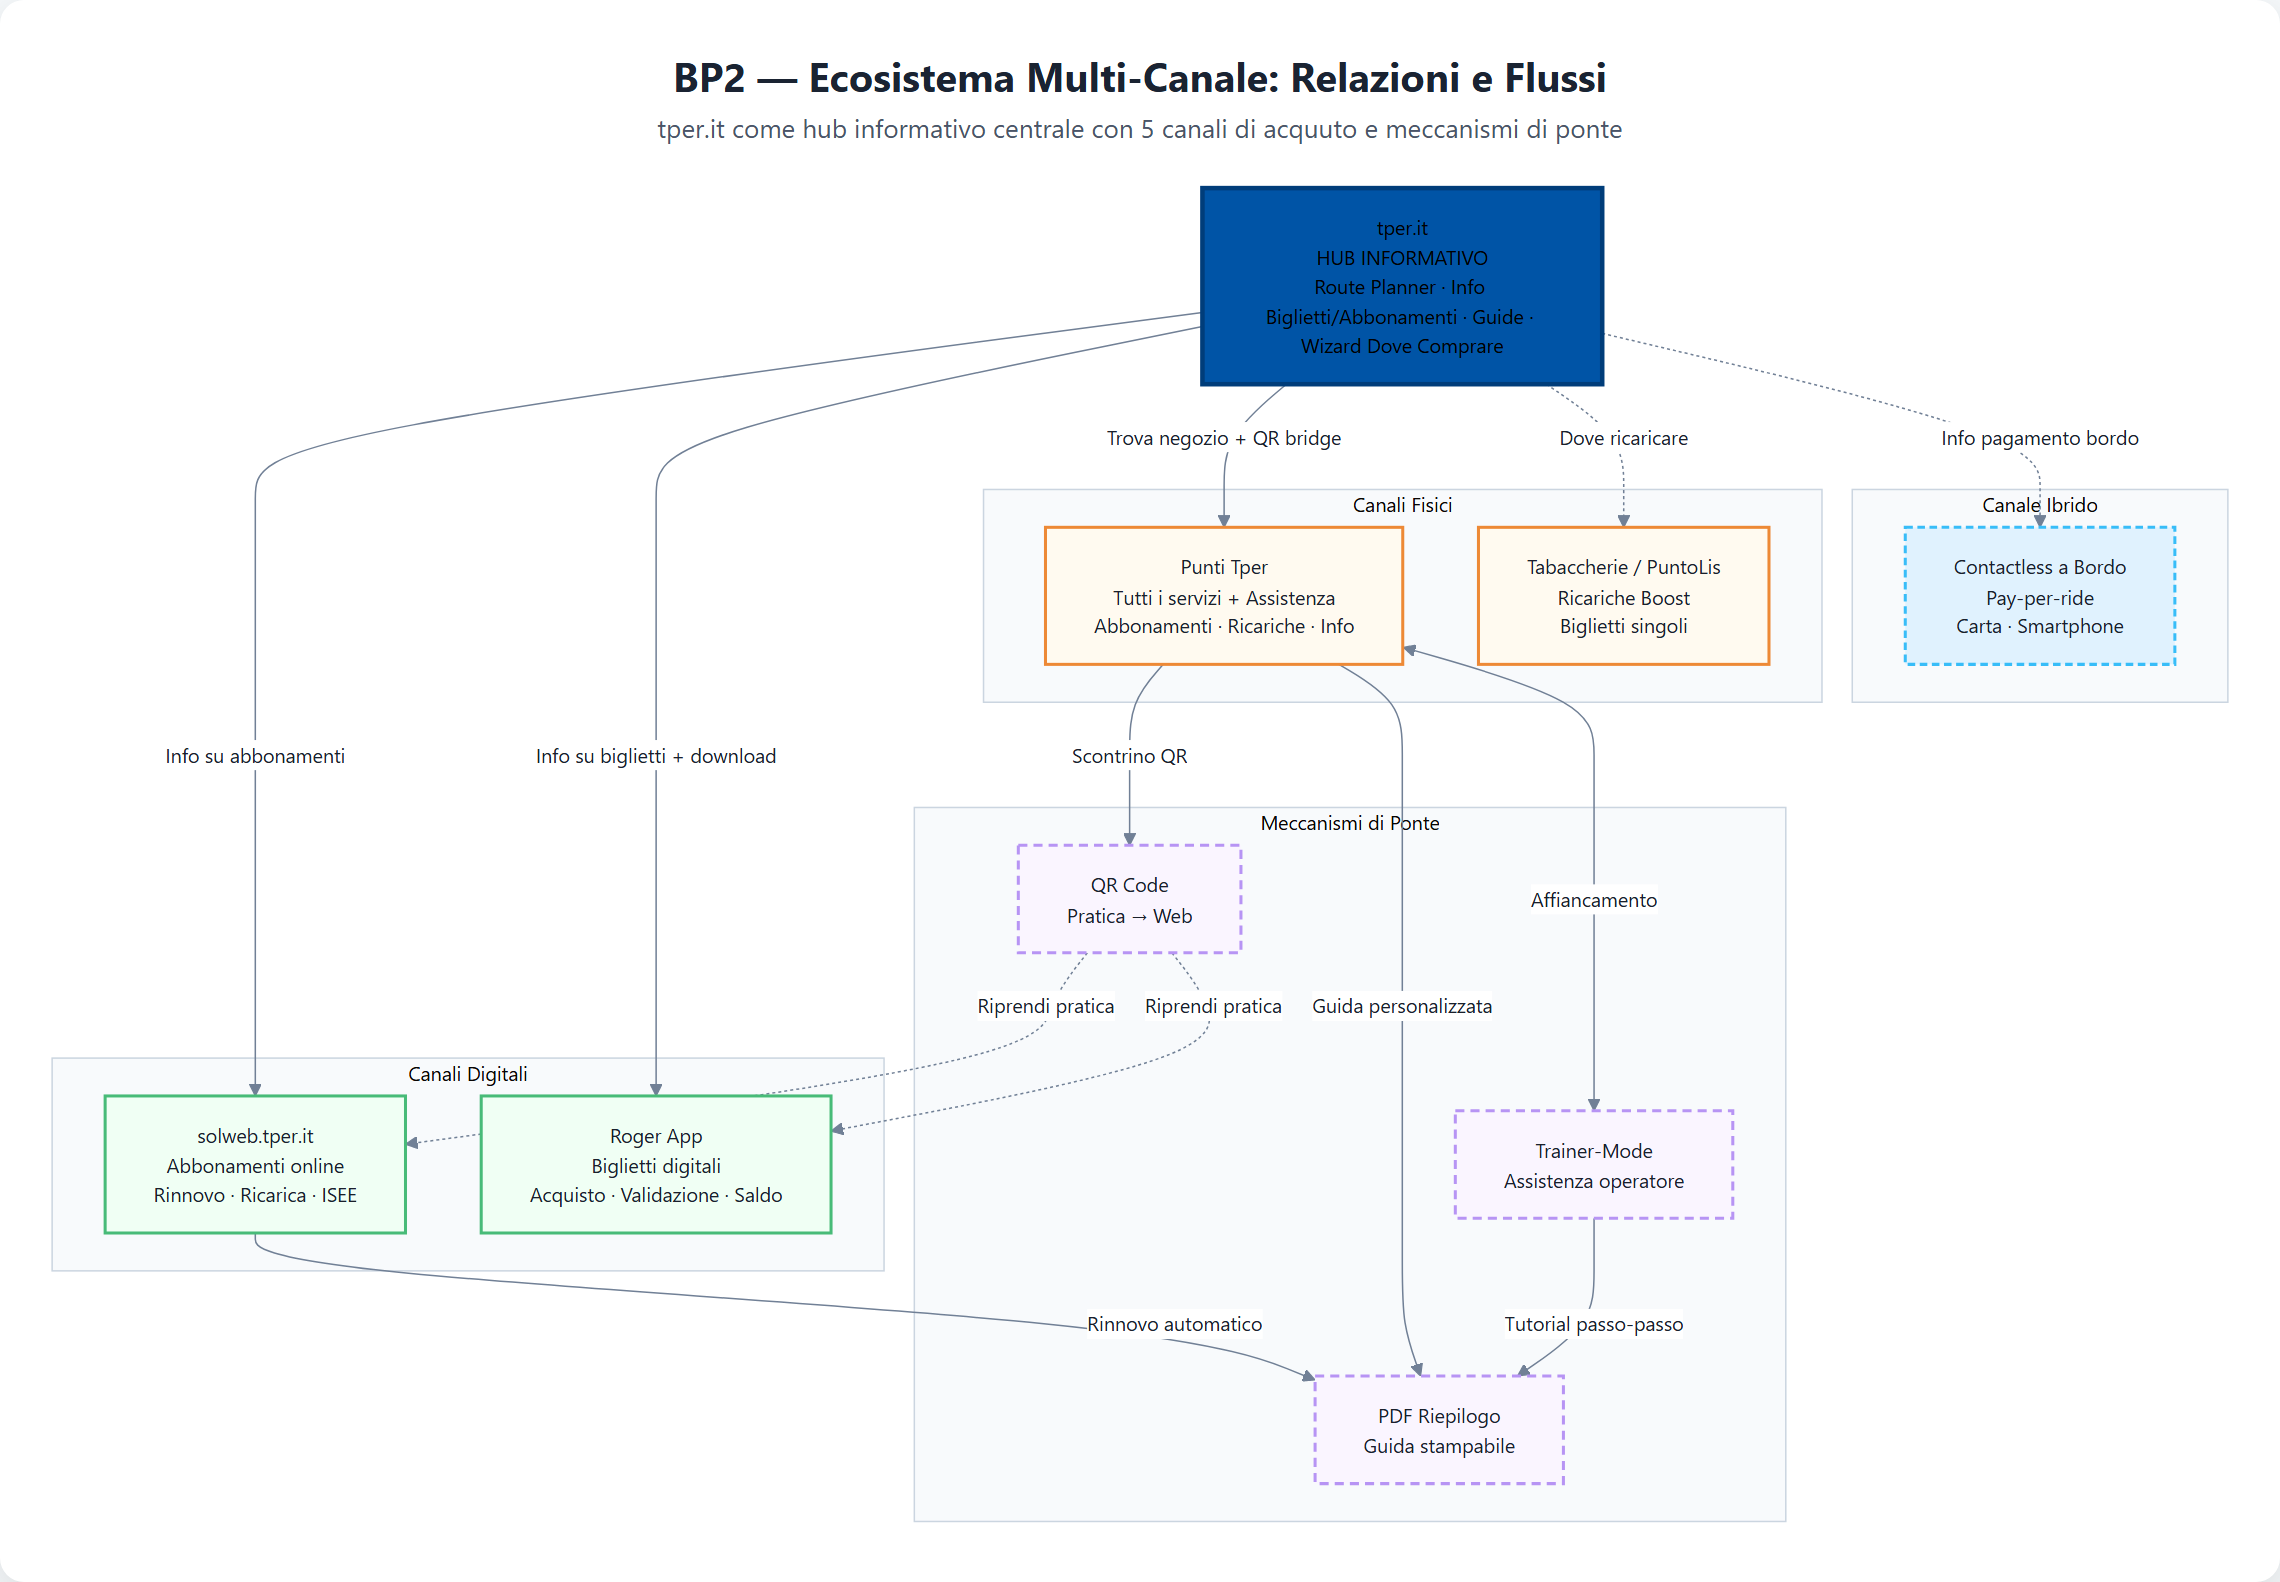
\includegraphics[width=\textwidth]{Blueprint/bp2-ecosystem.png}
\caption{BP2 --- TPER Multi-Channel Ecosystem}
\label{fig:bp2}
\end{figure}

\newpage

\subsubsection*{The 5 Purchase Channels}

\begin{table}[H]
\centering
\small
\renewcommand{\arraystretch}{1.3}
\begin{tabular}{|p{2.5cm}|p{3.5cm}|p{3.5cm}|p{3.5cm}|}
\hline
\textbf{Channel} & \textbf{Type} & \textbf{Functions} & \textbf{Access} \\
\hline
\texttt{solweb}\discretionary{-}{-}{.}\texttt{tper.it} & Digital & Online subscriptions, renewal, top-up, ISEE concessions & Web browser, requires account \\
\hline
Roger App & Digital & Digital tickets, purchase, validation, contact balance & Smartphone (iOS/Android) \\
\hline
Punti Tper & Physical & All services, assistance, top-ups, subscriptions & Physical counter \\
\hline
Tabaccherie / PuntoLis & Physical & Boost top-ups, single tickets & Authorized retailer \\
\hline
Contactless on board & Hybrid & Pay-per-ride with card or smartphone & On TPER vehicle \\
\hline
\end{tabular}
\caption{Overview of the 5 purchase channels of the TPER ecosystem}
\label{tab:canali}
\end{table}

\subsubsection*{Bridge Mechanisms}
\begin{itemize}
    \item \textbf{Web redirects}: External links from \texttt{tper.it} to \texttt{solweb.tper.it} and Roger App download pages
    \item \textbf{QR Code}: Receipt issued at Punti Tper with QR code to resume the procedure from home
    \item \textbf{Printed guides}: Automatically generated PDFs with the complete path (R6)
    \item \textbf{Trainer-Mode}: Counter operators guiding the user in channel selection
\end{itemize}

\vspace{0.3cm}

% =====================================================================
% BP3 --- USER JOURNEY
% =====================================================================
\section{BP3 --- User Journey: from tper.it to Purchase}

\textit{User perspective.} This blueprint traces the typical path of an HPHP user from the moment they arrive on \texttt{tper.it} until purchase completion on the correct channel.

\begin{figure}[H]
\centering
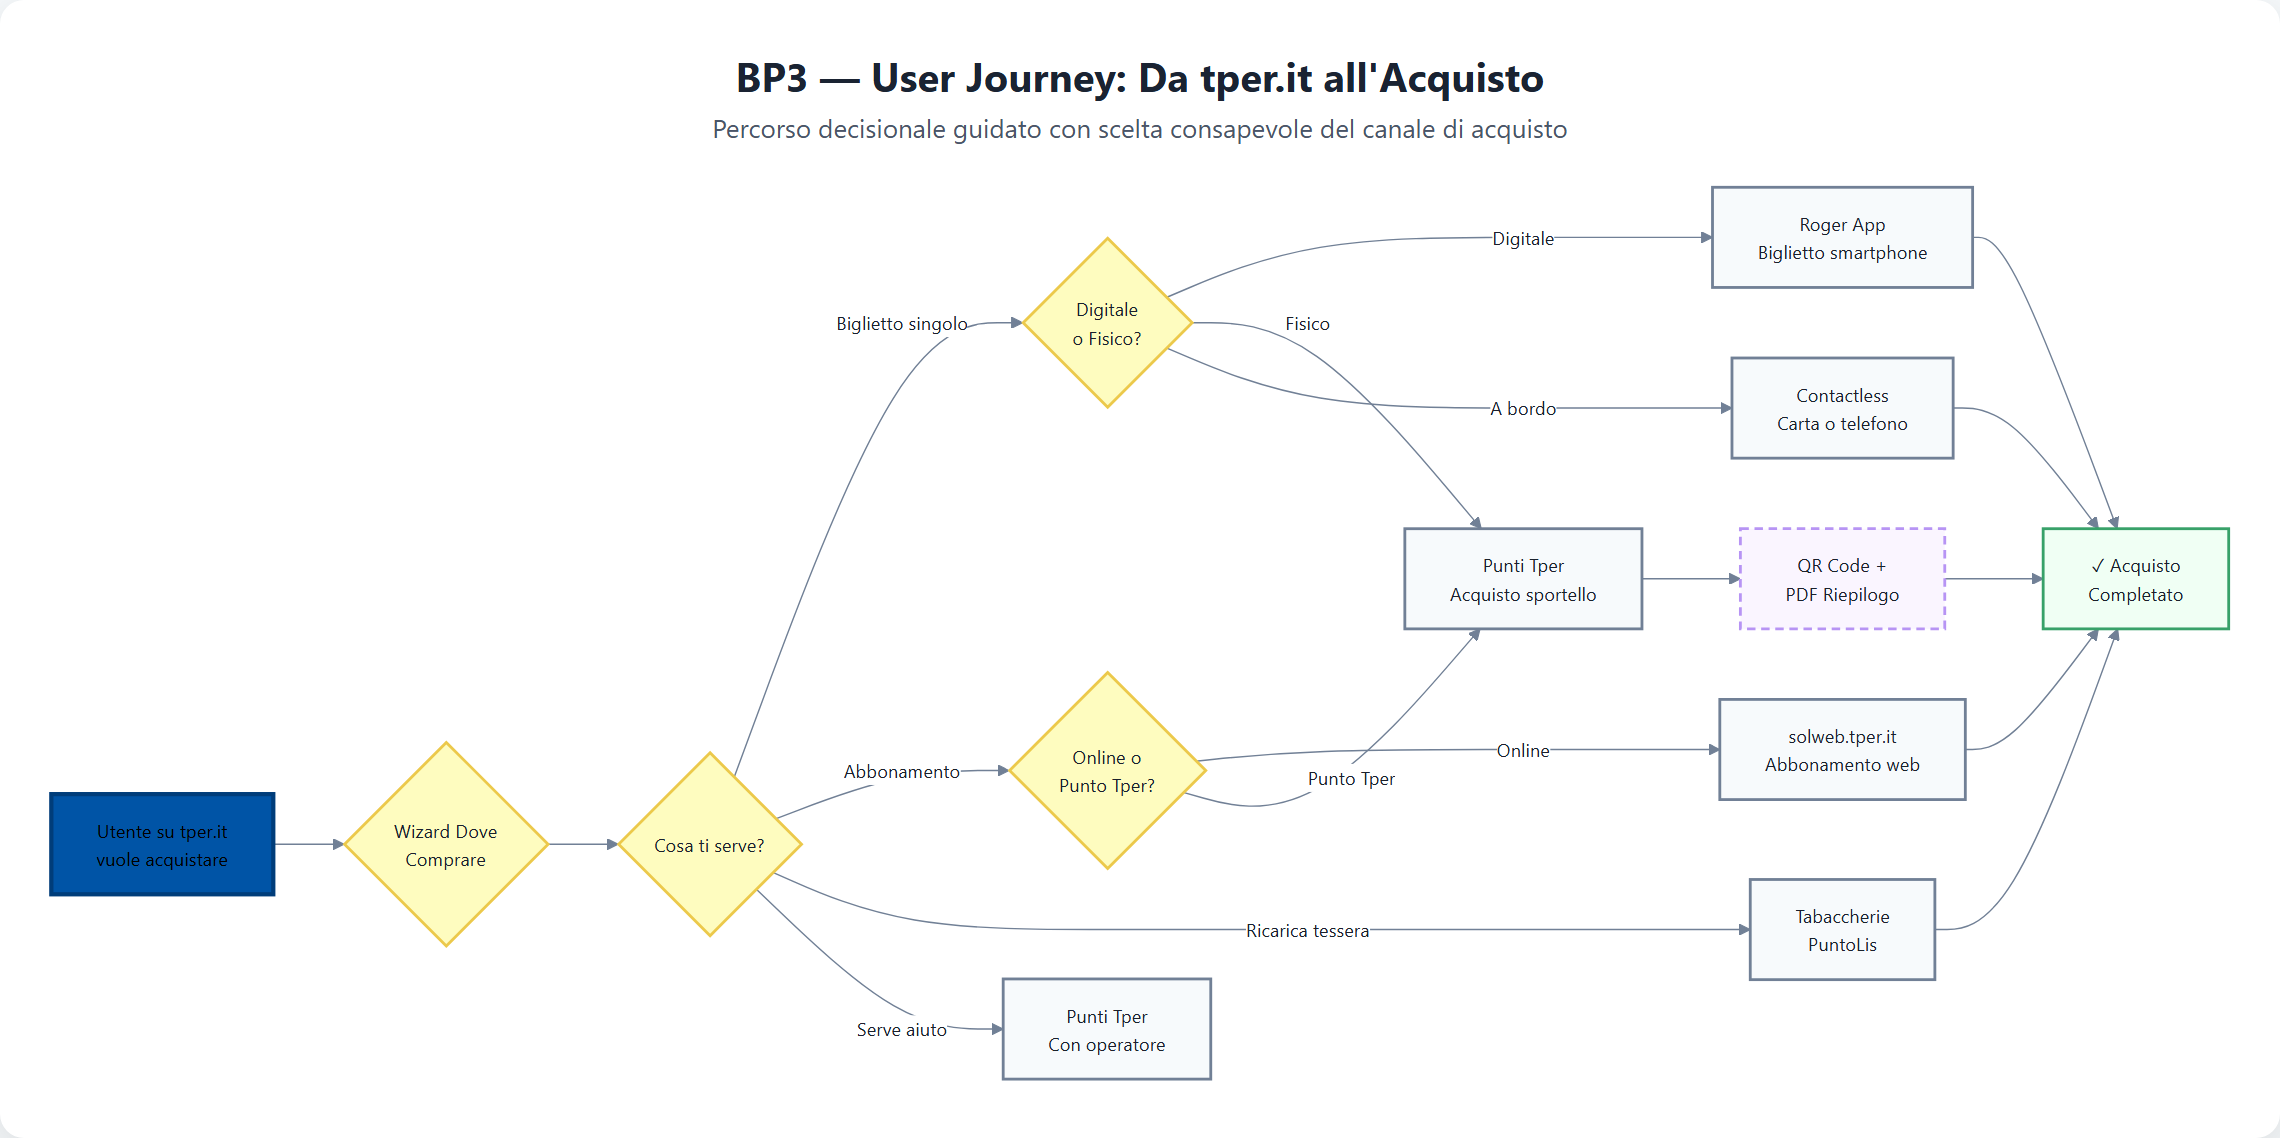
\includegraphics[width=\textwidth]{Blueprint/bp3-journey.png}
\caption{BP3 --- User Journey from \texttt{tper.it} to Purchase}
\label{fig:bp3}
\end{figure}

\subsubsection*{Decision Points}
\begin{enumerate}
    \item \textbf{Need to buy?}: Fork between users looking only for information (timetables, routes) and users who need to purchase.
    \item \textbf{Digital or Physical?}: Choice based on the user's digital preferences and skills.
    \item \textbf{Have an account?}: For the digital channel, distinction between those who already have a solweb account and those who need to use Roger App.
    \item \textbf{What do you need to do?}: For the physical channel, distinction between full purchase (Punti Tper), top-up (tobacconists), or on-board payment (contactless).
\end{enumerate}

\subsubsection*{Trainer-Mode Intervention}
The system activates the assisted mode (Trainer-Mode) in two cases:
\begin{itemize}
    \item \textbf{On request}: The user clicks ``Aiuto'' during the journey
    \item \textbf{After 2 consecutive errors}: The user shows difficulty in navigation or channel selection
\end{itemize}
Trainer-Mode provides: document checklist, channel selection guide, and step-by-step tutorial.

\vspace{0.5cm}

% =====================================================================
% SUMMARY
% =====================================================================
\section{Blueprint Summary}

\begin{table}[H]
\centering
\small
\renewcommand{\arraystretch}{1.3}
\begin{tabular}{|p{1.8cm}|p{3cm}|p{3.5cm}|p{5cm}|}
\hline
\textbf{Blueprint} & \textbf{Perspective} & \textbf{Stakeholders} & \textbf{Covered Elements} \\
\hline
BP1 & Structure & Developers, content managers & Page hierarchy, informational sections, redirects \\
\hline
BP2 & System & IT, product owner, marketing & Channel relationships, bridge mechanisms, types \\
\hline
BP3 & User & Designers, counter operators & Decision path, intervention points, trainer-mode \\
\hline
\end{tabular}
\caption{Overview of the three blueprints and their stakeholders}
\label{tab:riepilogo-bp}
\end{table}

\vspace{0.5cm}

\begin{center}
{\color{secondaryColor}\small
Document compiled based on evidence gathered during Phase A and Phase B \\[4pt]
\textbf{Phase C --- Design Proposal: Blueprint} \\[4pt]
Project: UX Design Project: Help People Help People --- TPER S.p.A.}
\end{center}

\vspace{0.3cm}

% ================================================================

\newpage

\subsection{Wireframe}

\begin{tcolorbox}[colback=primaryColor,colframe=primaryColor,arc=1.5mm,halign=center,valign=center,height=2cm]
 \color{white}\LARGE\bfseries\sffamily WIREFRAMES \\[0.1cm]
 \color{white!80}\small\sffamily Phase C --- Design Proposal
\end{tcolorbox}

\vspace{0.3cm}

The wireframes presented in this section illustrate the key screens of \textbf{tper.it}, the TPER informational portal. Contrary to what was previously assumed, \textbf{tper.it does not allow direct purchases}: it is an informational platform that supports the user in trip planning and in navigating between the physical and digital sales channels of the TPER ecosystem.

\vspace{0.2cm}
\textbf{TPER ecosystem channels:}
\begin{itemize}
    \item \textbf{tper.it} --- Informational: route planning, timetables, ticket types, news, contacts
    \item \textbf{solweb.tper.it} --- Portal for purchasing subscriptions online
    \item \textbf{Roger App} --- App for digital tickets and mobile payments
    \item \textbf{Punti Tper} --- Physical stores for all purchases
    \item \textbf{Tabaccherie / PuntoLis} --- Top-up points
    \item \textbf{Contactless on board} --- Payment per single ride with card
\end{itemize}

\vspace{0.2cm}
\textbf{Graphic conventions:}
\begin{itemize}
    \item Blue boxes = main interactive elements (CTA, navigation)
    \item Gray boxes = informational content / secondary areas
    \item Purple line = Trainer-Mode elements
    \item \texttt{Italic} text = descriptive labels
\end{itemize}

\newpage

% ================================================================
% WF1: HOMEPAGE tper.it (GUEST)
% ================================================================
\section{Wireframe 1: tper.it Homepage --- Unauthenticated User (Guest)}
\label{wf1}

\begin{figure}[H]
\centering
\wfgraphic{Wireframes/screenshot-wf1.png}
\caption{tper.it Homepage --- Unauthenticated user view (Guest)}
\label{fig:wf1}
\end{figure}

\newpage

% ================================================================
% WF2: PIANIFICA (ROUTE PLANNER)
% ================================================================
\section{Wireframe 2: Pianifica --- The Route (Core Function)}
\label{wf2}

\begin{figure}[H]
\centering
\wfgraphic{Wireframes/screenshot-wf2.png}
\caption{Pianifica --- Route search results with informational prices}
\label{fig:wf2}
\end{figure}

\newpage

% ================================================================
% WF3: DOVE COMPRARE (CHANNEL GUIDE)
% ================================================================
\section{Wireframe 3: Dove Comprare --- Channel Guide}
\label{wf3}

\begin{figure}[H]
\centering
\wfgraphic{Wireframes/screenshot-wf3.png}
\caption{Dove Comprare --- Sales channel guide with comparison table}
\label{fig:wf3}
\end{figure}

\newpage

% ================================================================
% WF4: BIGLIETTI (INFORMATIONAL)
% ================================================================
\section{Wireframe 4: Biglietti --- Types and Prices}
\label{wf4}

\begin{figure}[H]
\centering
\wfgraphic{Wireframes/screenshot-wf4.png}
\caption{Biglietti --- Types, prices, and recommended channels}
\label{fig:wf4}
\end{figure}

\newpage

% ================================================================
% WF5: AIUTO + TRAINER-MODE
% ================================================================
\section{Wireframe 5: Aiuto and Trainer-Mode --- Step-by-Step Guide}
\label{wf5}

\begin{figure}[H]
\centering
\wfgraphic{Wireframes/screenshot-wf5.png}
\caption{Aiuto and Trainer-Mode --- FAQ and activatable step-by-step guide}
\label{fig:wf5}
\end{figure}

\newpage

% ================================================================
% WF6: ABBONAMENTI + TRAINER (RENEWAL)
% ================================================================
\section{Wireframe 6: Abbonamenti --- Renewal Trainer}
\label{wf6}

\begin{figure}[H]
\centering
\wfgraphic{Wireframes/screenshot-wf6.png}
\caption{Abbonamenti --- Types and active Renewal trainer-mode with highlight}
\label{fig:wf6}
\end{figure}

\newpage

% ================================================================
% WF7a: SOLWEB PAYMENT
% ================================================================
\section{Wireframe 7a: solweb --- Payment Flow}
\label{wf7a}

\begin{figure}[H]
\centering
\wfgraphic{Wireframes/screenshot-wf7a.png}
\caption{solweb --- Payment with cart summary and payment method}
\label{fig:wf7a}
\end{figure}

\newpage

% ================================================================
% WF7b: SOLWEB CONFIRMATION
% ================================================================
\section{Wireframe 7b: solweb --- Post-Purchase Confirmation}
\label{wf7b}

\begin{figure}[H]
\centering
\wfgraphic{Wireframes/screenshot-wf7b.png}
\caption{solweb --- Confirmation screen with summary and next options}
\label{fig:wf7b}
\end{figure}

\vspace{0.5cm}

% ================================================================
% SUMMARY TABLE
% ================================================================
\section{Wireframe Summary}

\begin{table}[H]
\centering
\small
\renewcommand{\arraystretch}{1.3}
\begin{tabular}{|p{2cm}|p{3cm}|p{4cm}|p{4.5cm}|}
\hline
\textbf{Wireframe} & \textbf{Screen} & \textbf{Main Content} & \textbf{Key Elements} \\
\hline
WF1 & Homepage Guest & Route planner, 4 informational cards (Pianifica, Biglietti, Abbonamenti, Aiuto), Dove Comprare sidebar & Nav tabs, hero search, channels in sidebar, news, contacts \\
\hline
WF2 & Pianifica & Route search form, results with timetables/duration/price, map/list toggle & Core function, Dove Comprare link for each result, informational prices \\
\hline
WF3 & Dove Comprare & 5 channel cards (solweb, Roger, Punti Tper, Tabaccherie, Contactless), comparison table & Cards with CTA, comparison by need, no direct purchase \\
\hline
WF4 & Biglietti & Ticket types with prices and validity, recommended badge, channel legend & Purely informational, channel icons per type, updated prices \\
\hline
WF5 & Aiuto + Trainer-Mode & FAQ by channel, guides section, trainer-mode toggle, 5-step guide & ON/OFF toggle, visible step-by-step, channel indicated for each step \\
\hline
WF6 & Abbonamenti & Subscription types, recommended badge, active Renewal trainer-mode & Trainer highlight, plan comparison, CTA per channel \\
\hline
WF7a & solweb Payment & Cart summary, payment method, card/data form & Transactional flow, breadcrumb, amount summary \\
\hline
WF7b & solweb Confirmation & Purchase confirmation, order summary, next options & Purchased ticket/subscription, print CTA, dashboard \\
\hline
\end{tabular}
\caption{Summary of wireframes produced (tper.it + solweb.tper.it)}
\label{tab:wfsum}
\end{table}

\vspace{0.3cm}

\begin{tcolorbox}[colback=primaryColor!5,colframe=primaryColor,arc=2mm]
\small
\textbf{Important note:} tper.it is an exclusively \textbf{informational} portal. There are no purchase, payment, or transaction flows. Each screen directs the user to the correct channel (\texttt{solweb.tper.it}, Roger App, Punti Tper, Tabaccherie, Contactless on board) to complete the desired operation. This architecture respects the actual channel separation in the TPER ecosystem.
\end{tcolorbox}

% ================================================================
% Comparison Before/After
% ================================================================

\newpage
\section{Comparison Before/After}
\label{sec:comparison}


\begin{tcolorbox}[colback=primaryColor,colframe=primaryColor,arc=3mm,halign=center,valign=center,height=2.5cm]
    \color{white}\LARGE\bfseries BEFORE/AFTER COMPARISON \\[0.2cm]
    \color{white!80}\large UX Design Project: Help People Help People --- TPER S.p.A. \\[0.1cm]
    \color{white!60}\normalsize Phase C --- Design Proposal
\end{tcolorbox}

\vspace{0.5cm}

\section{Introduction}

This Before/After comparison highlights the differences between the current \texttt{tper.it} site and the \texttt{tper 2.0} redesign proposal, developed from the 13 recommendations R1--R13 (Phase B). Each section is anchored to Phase A evidence: 4 subjects tested, only \textbf{6/20 tasks completed (30\%)}, \textbf{average SUS 37.5/100} --- well below the acceptability threshold. Use cases UR-01--UR-05 guided the design decisions.

\vspace{0.2cm}

\textbf{TPER Ecosystem:} \texttt{tper.it} is a \textit{purely informational} site --- it does not allow direct purchases. Transactions occur across 5 specialised channels:
\begin{itemize}[nosep]
    \item \texttt{solweb.tper.it} --- online subscriptions;
    \item \textbf{Roger App} --- digital tickets;
    \item \textbf{Punti Tper} --- physical counters;
    \item \textbf{Tobacconists / PuntoLis} --- top-ups;
    \item \textbf{Contactless onboard} --- instant payment.
\end{itemize}
The redesign transforms \texttt{tper.it} from a generic news container into an \textbf{informational hub and active ecosystem guide}.

\vspace{0.3cm}

% ============================================================
% COMPARISON 1: tper.it HOMEPAGE
% ============================================================
\section{\texttt{tper.it} Home Page}
\label{sec:comparison-home}

\textbf{D1 $\rightarrow$ R1} --- Chaotic homepage (P5,I5) $\rightarrow$ Task-oriented. Maria: \textit{``I don't know where to start''}, avg SUS 37.5/100.

\begin{figure}[H]
\centering
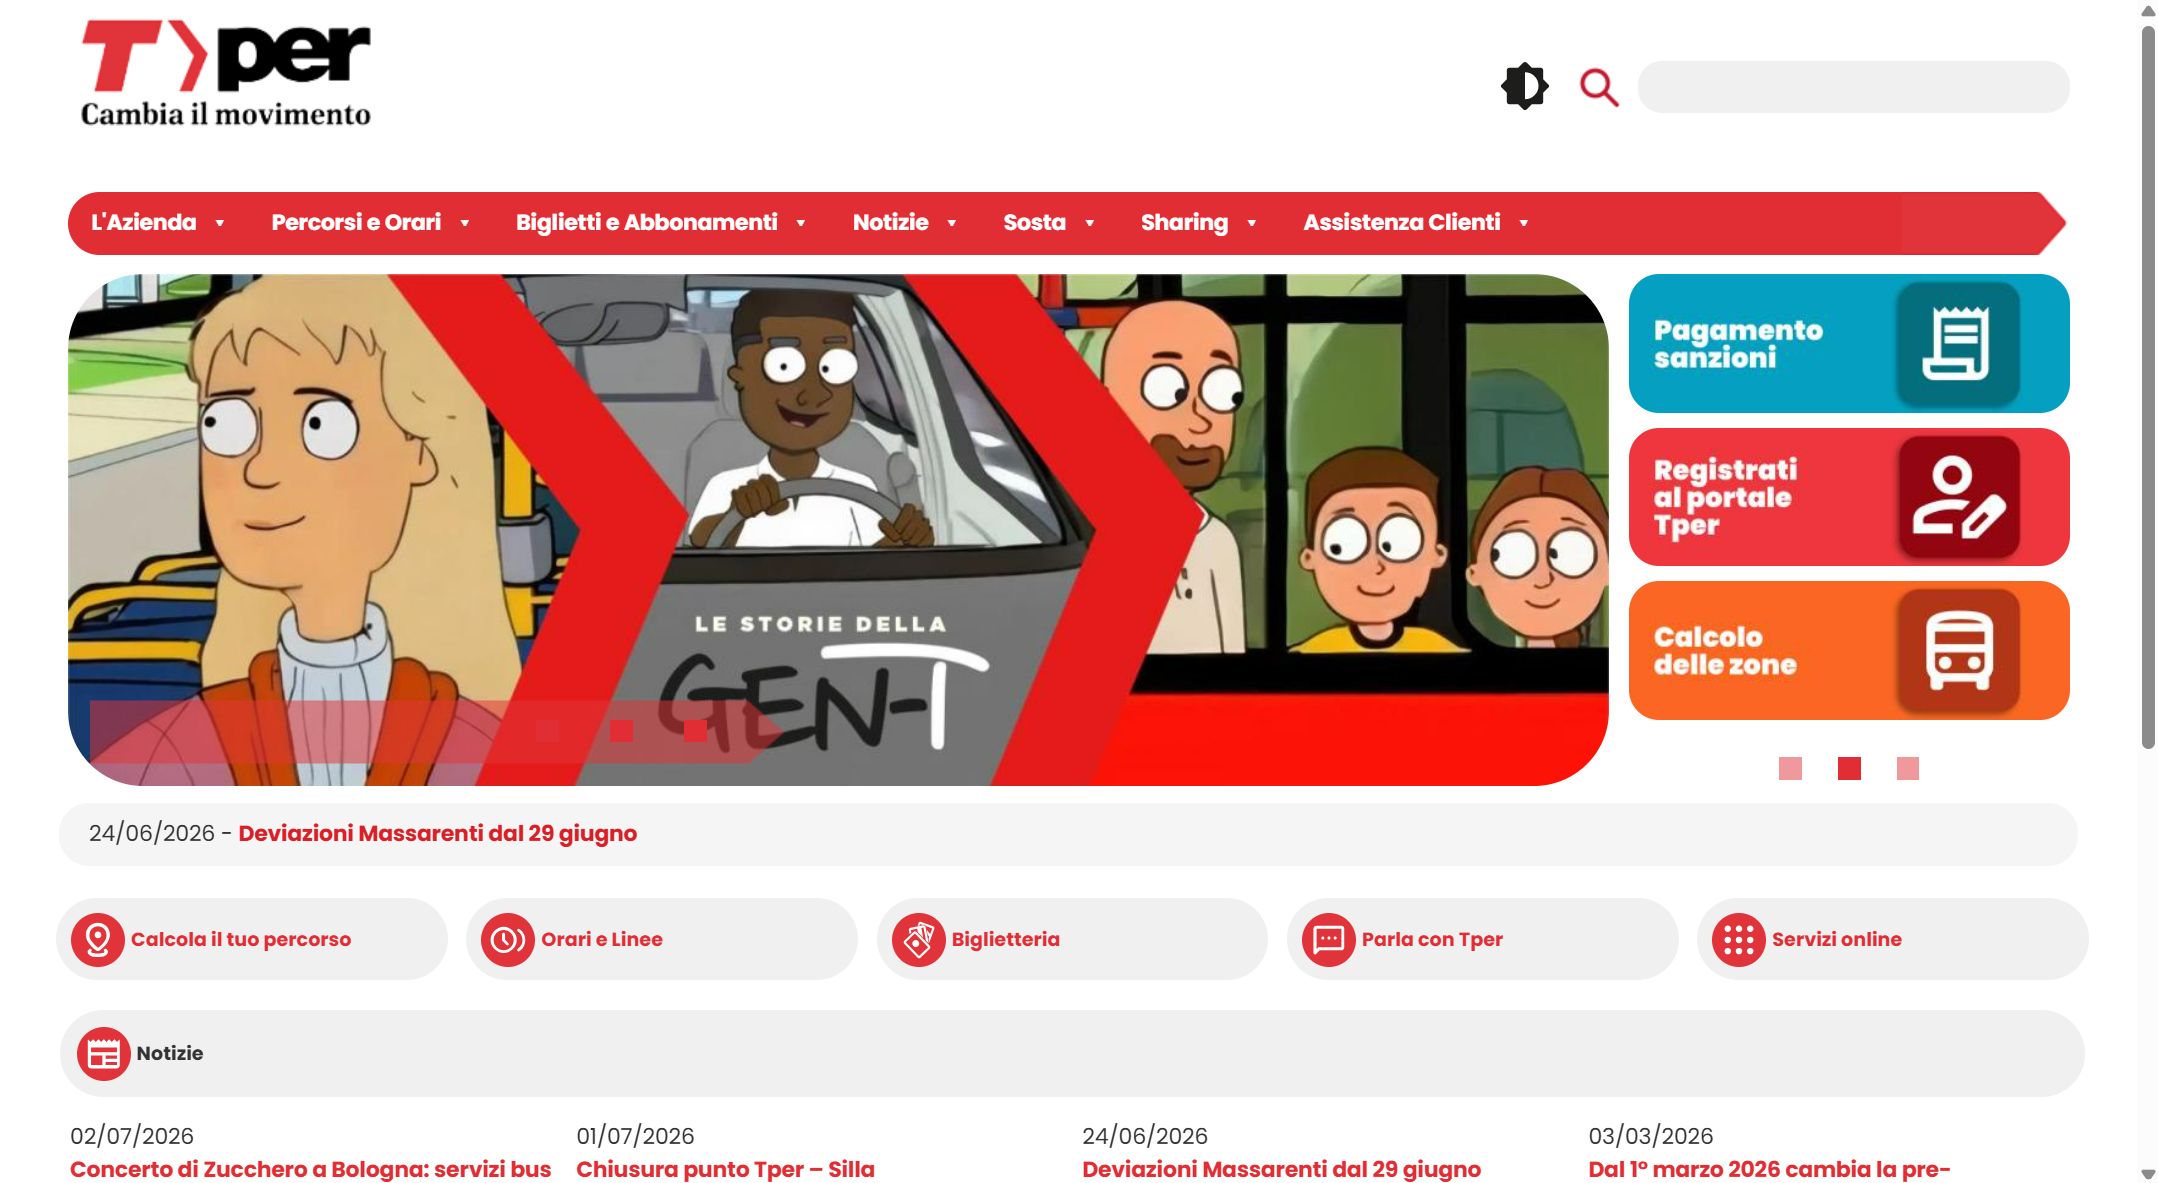
\includegraphics[width=0.85\textwidth]{Tper sito originale/Homepage.png}
\par\small\textit{Before: \texttt{tper.it} live --- corporate news slider, no primary CTA}
\vspace{0.4cm}
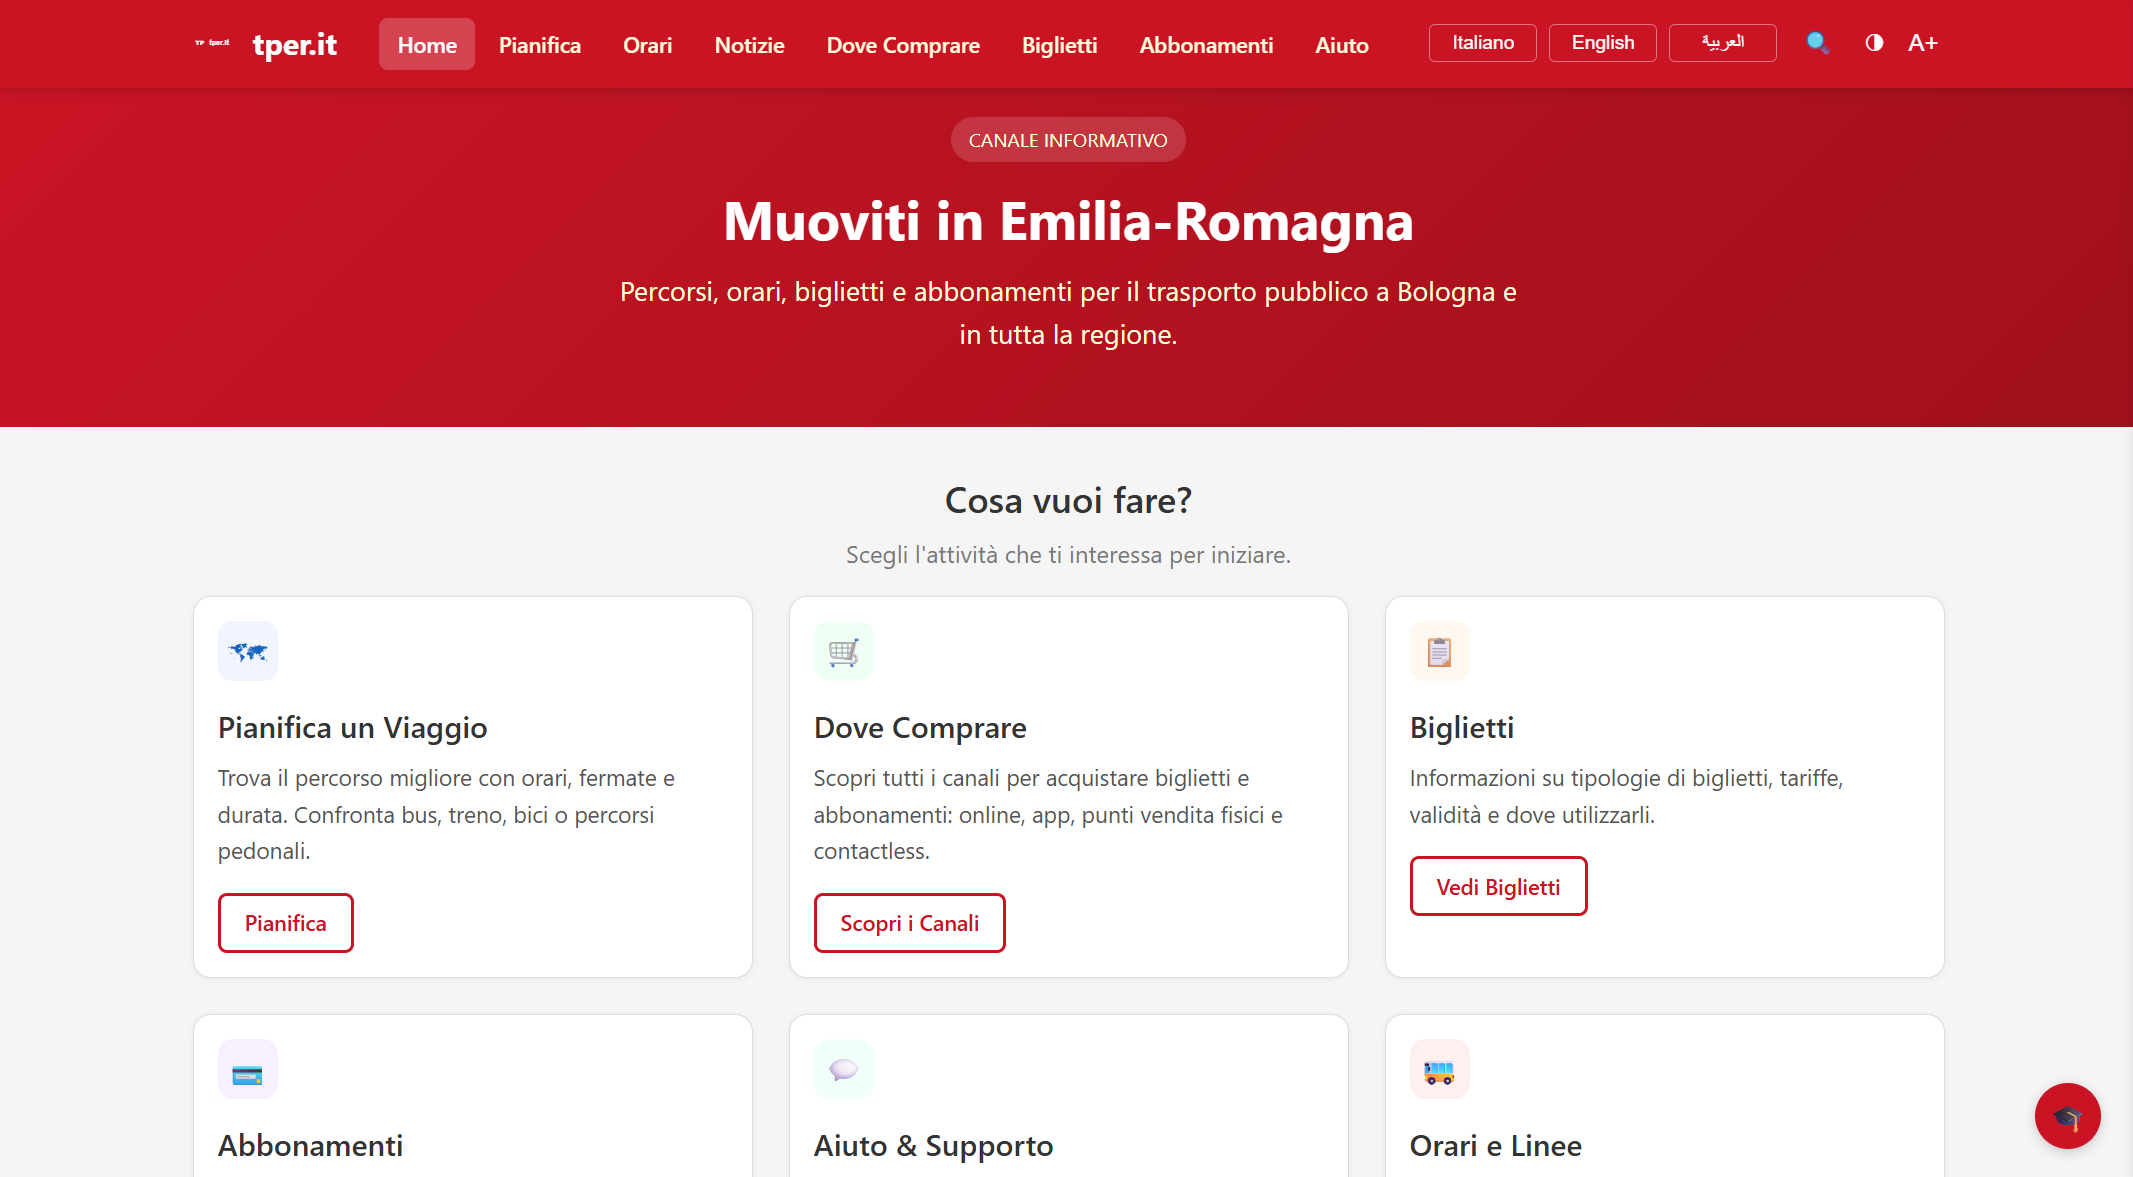
\includegraphics[width=0.85\textwidth]{Redesign Tper 2.0/homepage.png}
\par\small\textit{After: tper 2.0 --- hero route planner + 6 task-oriented cards grid}
\caption{\texttt{tper.it} Homepage}
\label{fig:comparison-home}
\end{figure}

\begin{table}[H]
\centering
\small
\renewcommand{\arraystretch}{1.4}
\begin{tabular}{|p{0.5cm}|p{7cm}|p{7cm}|}
\hline
& \textbf{Before} & \textbf{After} \\ \hline
\cellcolor{primaryColor!15} &
\textit{Current \texttt{tper.it} homepage (live)} &
\textit{\texttt{tper 2.0} redesign homepage} \\ \hline

\raisebox{0.5cm}{\rotatebox{90}{\textbf{Content}}} &
Corporate news slider, press releases, tender notices occupy the homepage. The trip planner is reachable after 2--3 clicks through \textit{Routes and Timetables} $\rightarrow$ \textit{Calculate your route}. No hierarchy between user content and institutional content (Issue D1). &
Hero section dedicated to the trip planner with ``From'' and ``To'' fields already visible. ``What do you want to do?'' grid with 6 task-oriented cards: Plan, Where to Buy, Tickets, Subscriptions, Help, Timetables. Corporate news moved to a separate section (R1). \\ \hline

\raisebox{0.5cm}{\rotatebox{90}{\textbf{CTAs}}} &
Generic text links: ``Online Services'', ``Routes and Timetables'', ``Ticketing'', ``Talk to Tper''. The user must interpret corporate terminology to understand where to go (Issue D3). &
Large buttons with icons and user language: ``Plan a Trip'', ``Where to Buy?'', ``View Tickets'', ``Discover Subscriptions'', ``Go to Help'', ``Check Timetables''. Each card shows a distinctive coloured icon (R2, R9). \\ \hline

\raisebox{0.5cm}{\rotatebox{90}{\textbf{Navigation}}} &
Mega-menu with 7 main items and over 50 sub-items, dominated by institutional content: \textit{Transparent Company}, \textit{Procurement and Suppliers}, \textit{The Company} occupy most of the space. The user gets lost among legal content (Issue D2). &
Flat navigation with 8 task-oriented items: Home, Plan, Timetables, News, \textbf{Where to Buy}, Tickets, Subscriptions, Help. Breadcrumb on all internal pages for orientation. Institutional content available via footer (R2, R3). \\ \hline

\raisebox{0.5cm}{\rotatebox{90}{\textbf{Info}}} &
No indication of the site's informational role. The user searches for transactional functions that do not exist on \texttt{tper.it} (UR-01, UR-03). &
Explicit banner on every page: ``\texttt{tper.it} is an informational website. To purchase tickets and subscriptions please use one of the dedicated channels'' with a link to Where to Buy. Hero badge: ``INFORMATIONAL CHANNEL'' (R1). \\ \hline
\end{tabular}
\caption{Homepage (\texttt{tper.it} live vs tper 2.0)}
\label{tab:comparison-home}
\end{table}

\vspace{0.3cm}

% ============================================================
% COMPARISON 2: solweb HOMEPAGE
% ============================================================
\section{\texttt{solweb.tper.it} Home Page}
\label{sec:comparison-solweb-home}

\textbf{D5 $\rightarrow$ R7} --- Mandatory login (P3,I5) $\rightarrow$ Guest path + 4 quick actions. 3/4 failed T3, unsignalled \texttt{tper.it}$\rightarrow$\texttt{solweb} transition.

\begin{figure}[H]
\centering
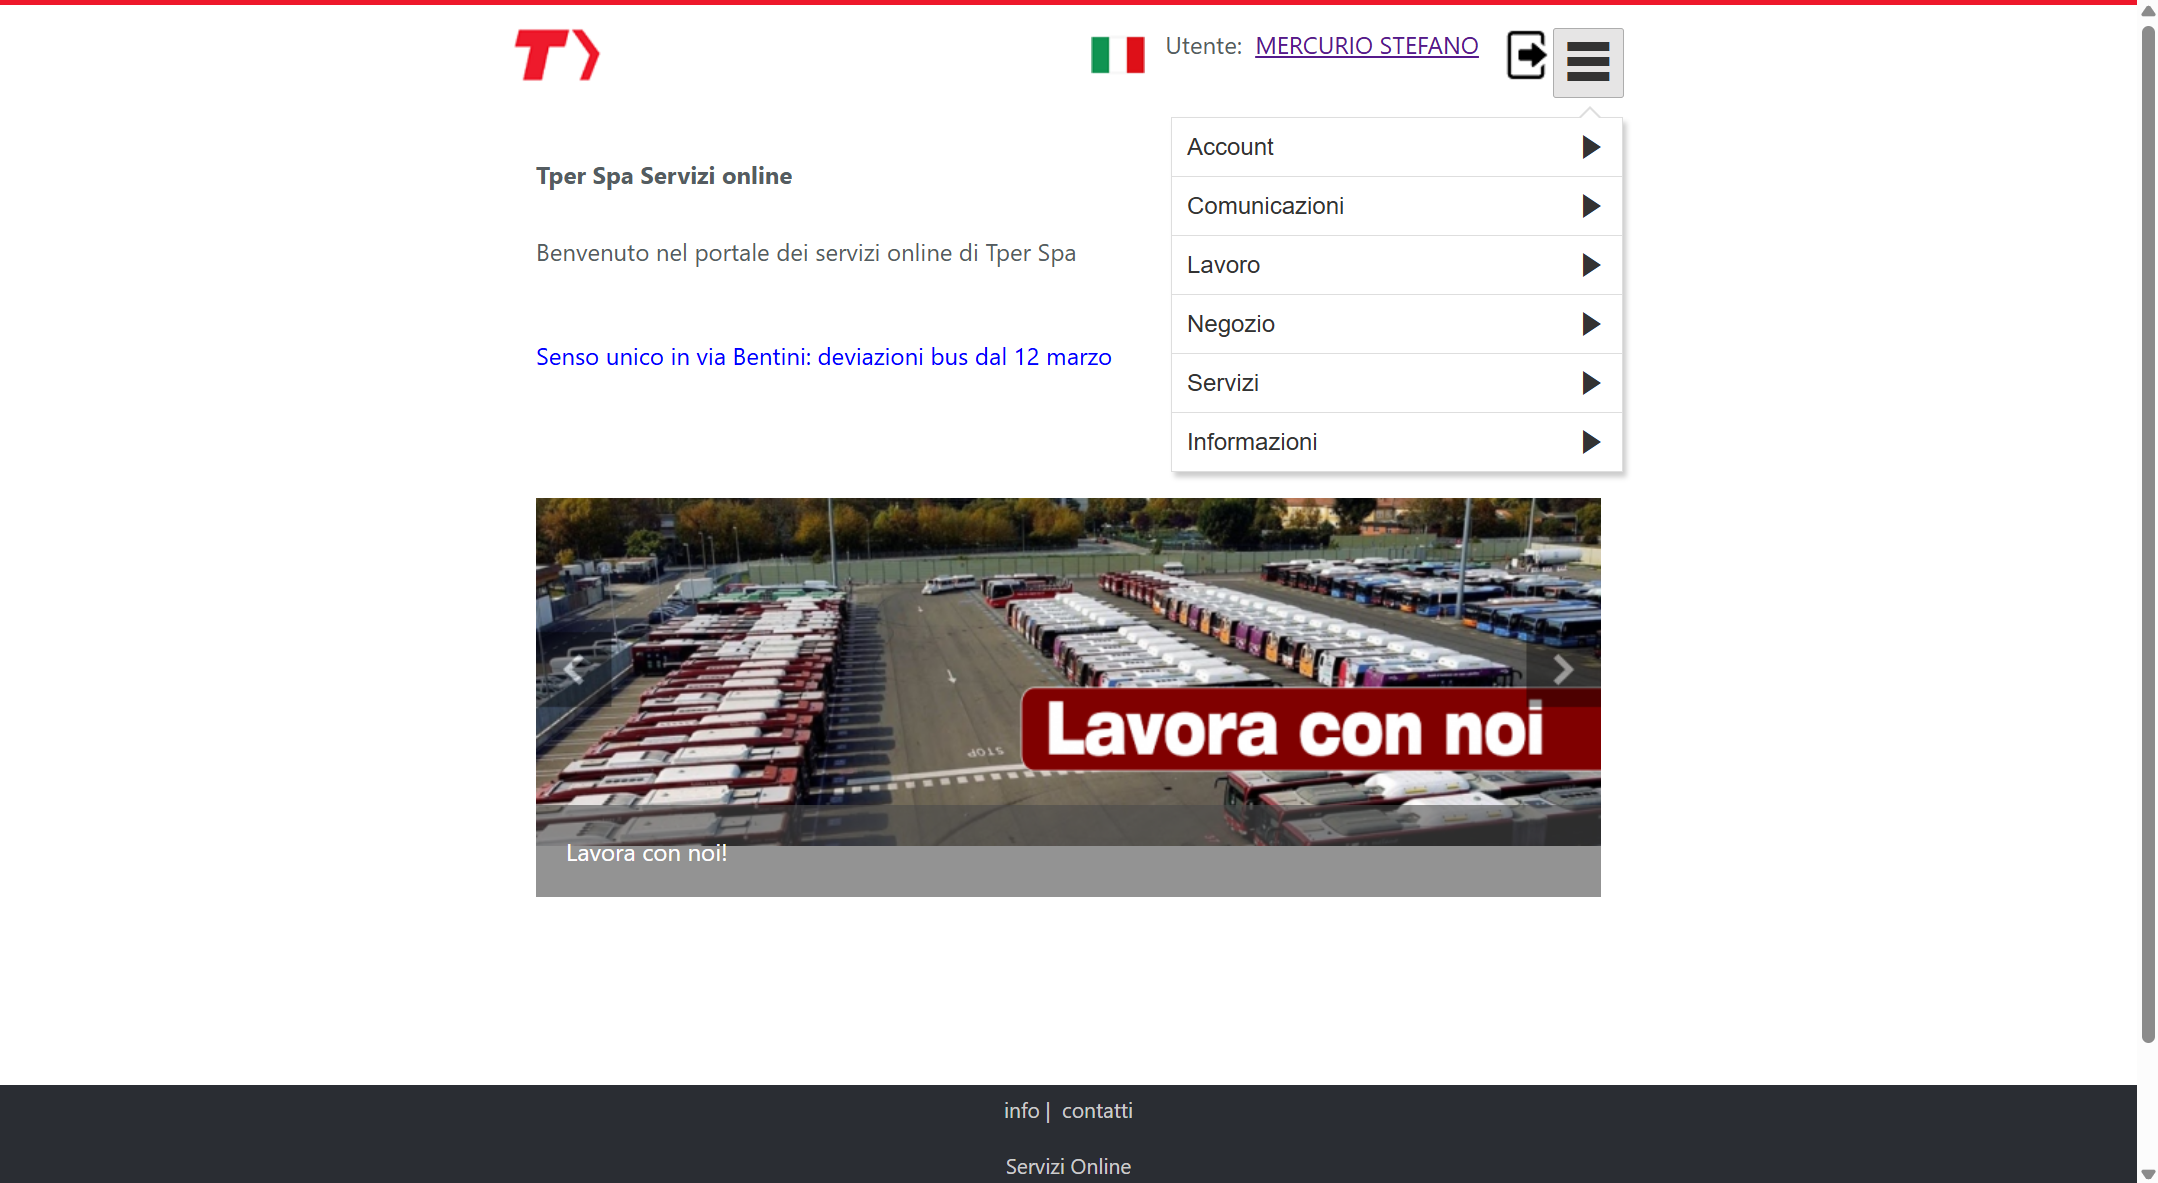
\includegraphics[width=0.85\textwidth]{Tper sito originale/HomepageS.png}\\[2pt]
{\small\textit{+ second view:}}\\[2pt]
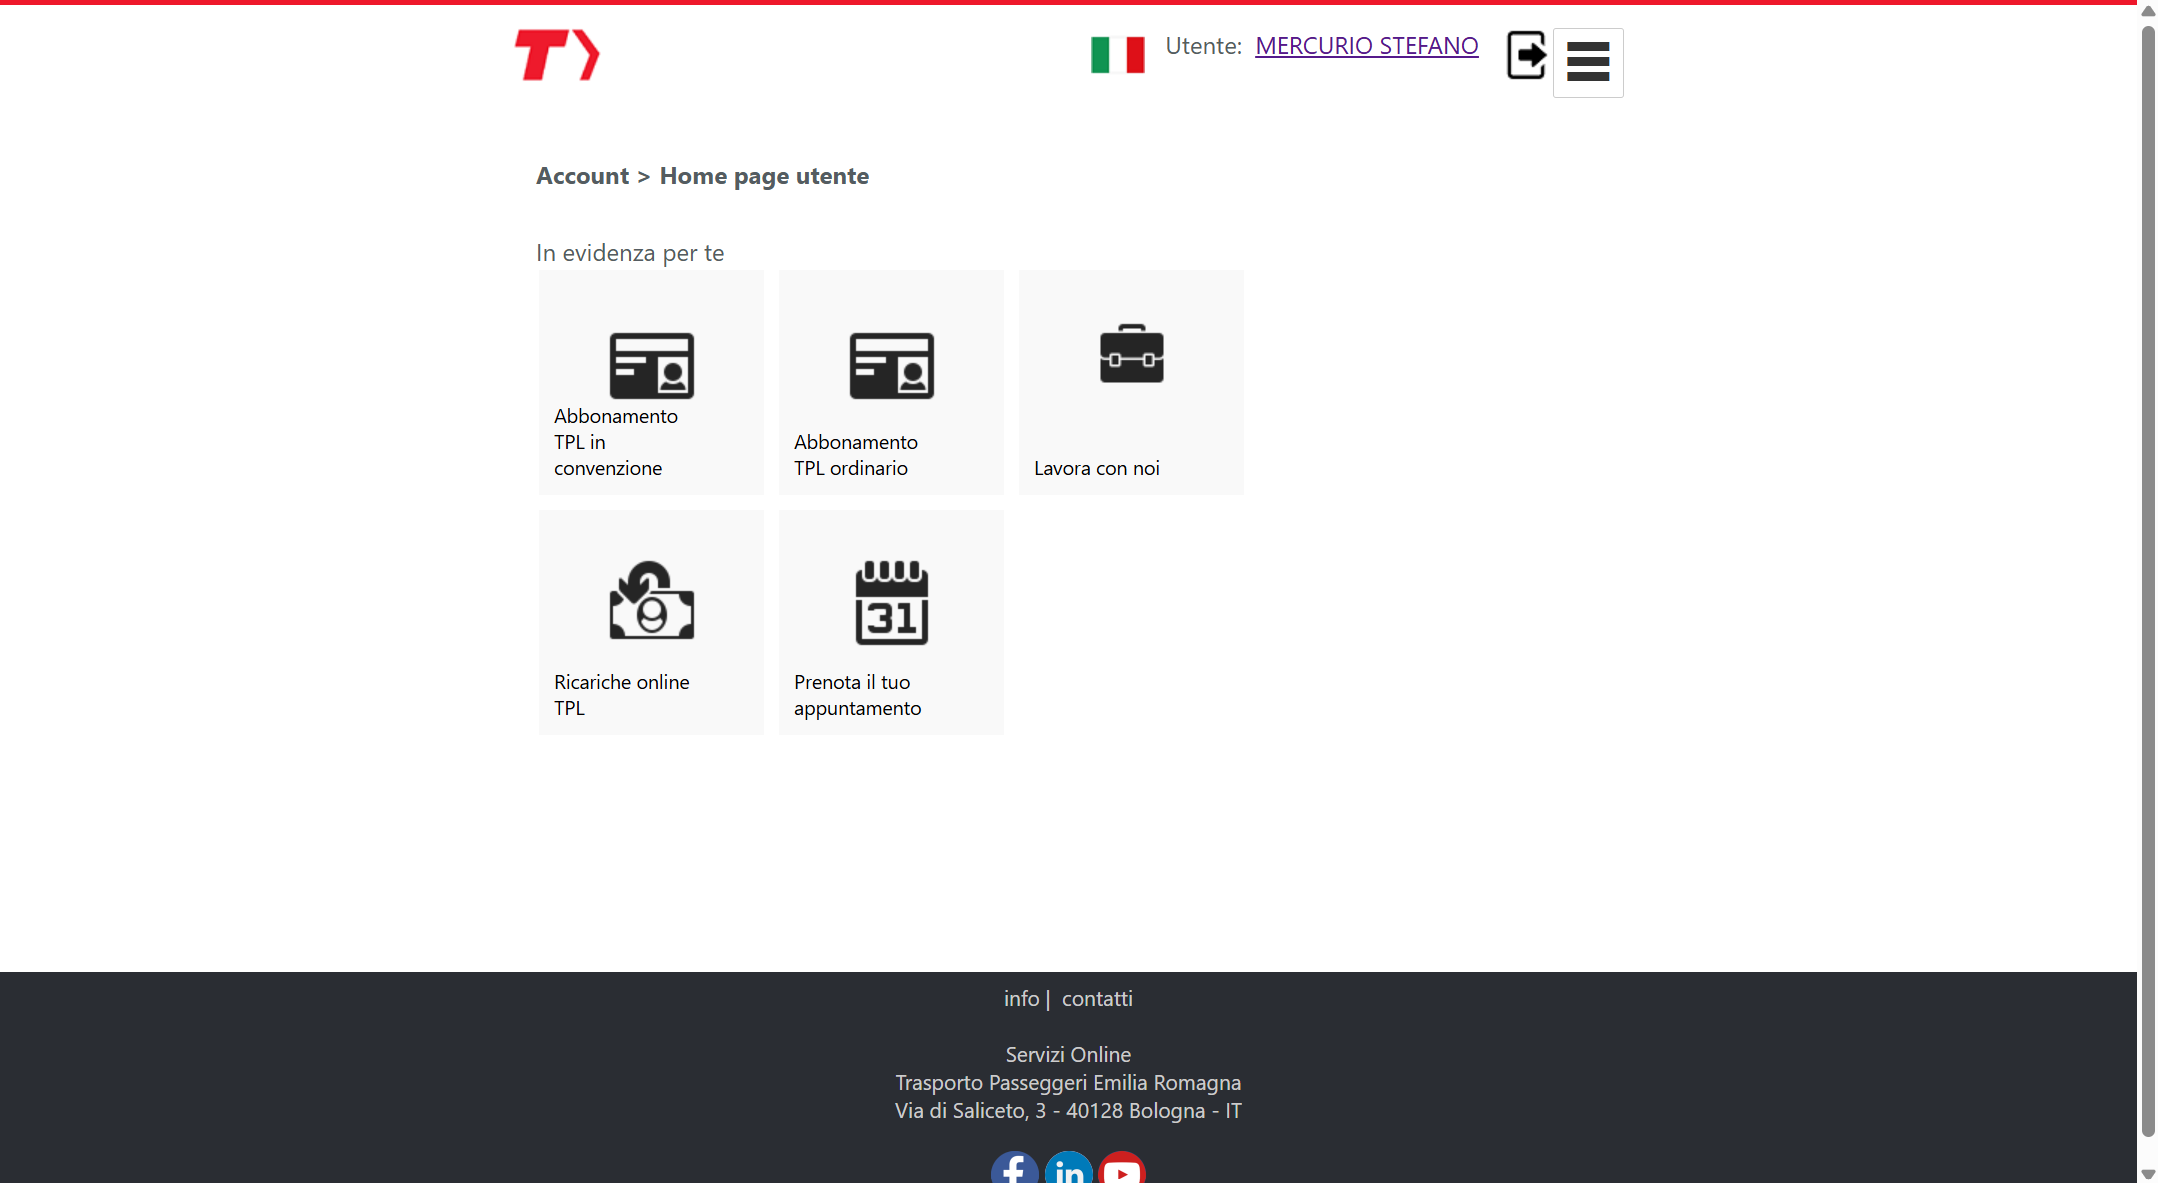
\includegraphics[width=0.85\textwidth]{Tper sito originale/HomepageS2.png}
\par\small\textit{Before: original \texttt{solweb} --- mandatory login, no guest path}
\vspace{0.4cm}
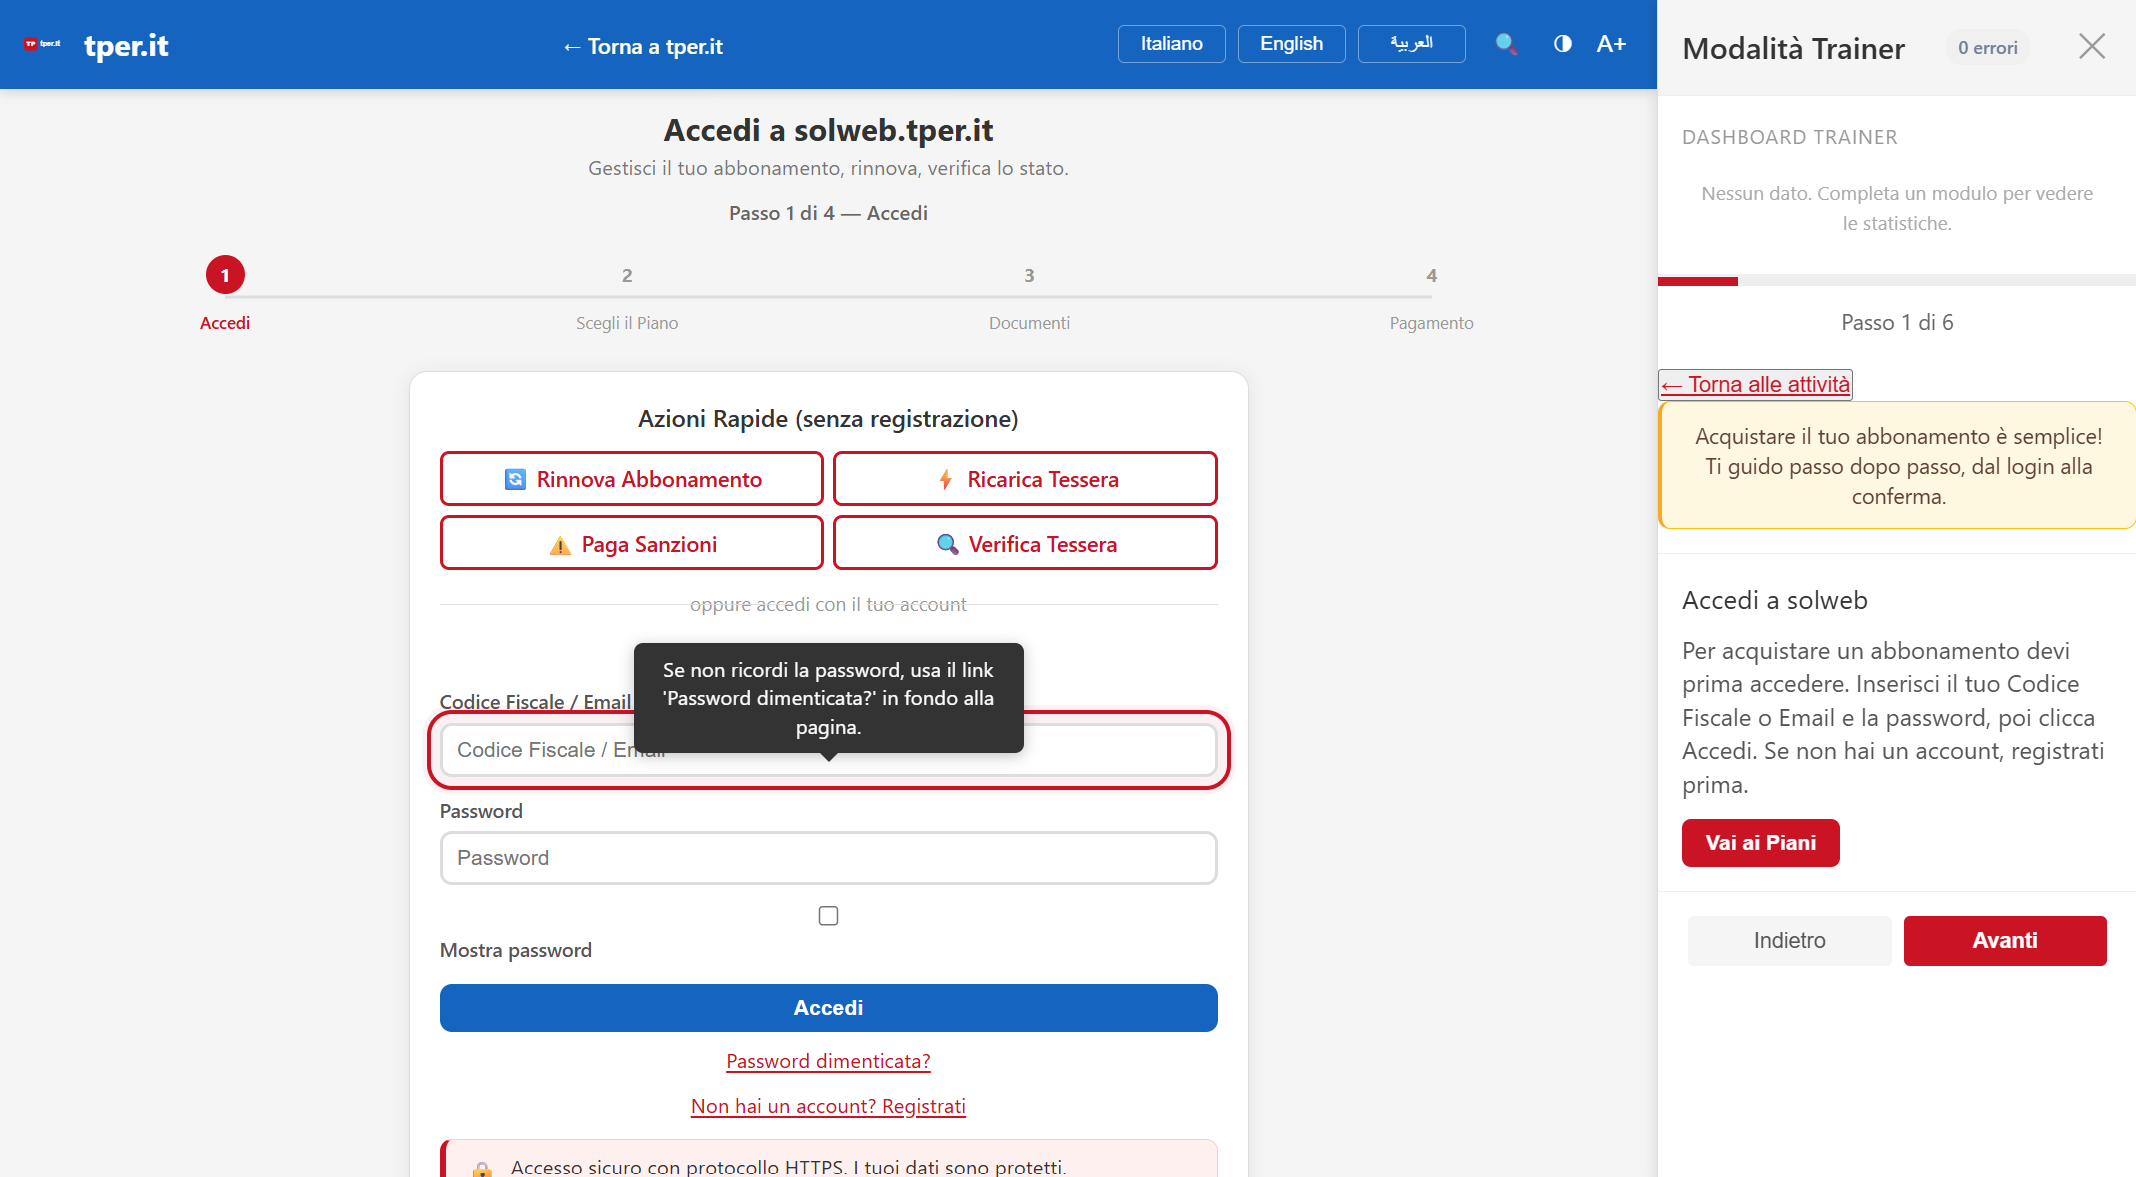
\includegraphics[width=0.85\textwidth]{Redesign Tper 2.0/HomepageS.png}
\par\small\textit{After: solweb 2.0 --- login + 4 quick actions without registration}
\caption{\texttt{solweb.tper.it} Homepage}
\label{fig:comparison-solweb-home}
\end{figure}

\begin{table}[H]
\centering
\small
\renewcommand{\arraystretch}{1.4}
\begin{tabular}{|p{0.5cm}|p{7cm}|p{7cm}|}
\hline
& \textbf{Before} & \textbf{After} \\ \hline
\cellcolor{primaryColor!15} &
\textit{Original solweb portal} &
\textit{solweb 2.0 in the redesign} \\ \hline

\raisebox{0.5cm}{\rotatebox{90}{\textbf{Access}}} &
\textbf{Login only}: username/SPID/CIE required for any operation. No guest alternative. For an elderly user with low digital competence, the mere request to ``create an account'' causes immediate abandonment (Issue D5). &
\textbf{4 quick actions without login}: Impersonal Renewal, Card Top-up, Pay Fines, Verify Card. Login remains available for operations requiring authentication (ISEE, personal subscriptions). 4-step progress bar: Login $\rightarrow$ Choose Plan $\rightarrow$ Documents $\rightarrow$ Payment (R7). \\ \hline

\raisebox{0.5cm}{\rotatebox{90}{\textbf{Transition}}} &
Switch from \texttt{tper.it} to \texttt{solweb} with no warning: domain, interface, colours, and layout all change. The user does not know if they are still on TPER (Issue R4). &
\textbf{Transition modal} before every external link: ``You are about to leave \texttt{tper.it} --- You will be redirected to the external purchase channel'' with the destination URL visible (R9). Solweb header with ``$\leftarrow$ Back to tper.it'' link always visible. \\ \hline

\raisebox{0.5cm}{\rotatebox{90}{\textbf{Orientation}}} &
No indication of where one is within the ecosystem. Interface completely different from \texttt{tper.it}, zero continuity signage. &
Blue header (\#1565C0) distinct from TPER red to signal the platform change. Hero badge ``SUBSCRIPTION PLATFORM'' in the dashboard. Contextual breadcrumbs. \\ \hline

\raisebox{0.5cm}{\rotatebox{90}{\textbf{Operations}}} &
All operations require registration. No distinction between simple operations (top-up, fines) and complex ones (ISEE, personal renewal). &
\textbf{Guest/authenticated separation}: top-up, fines, and card verification accessible without login. Purchase and personal renewal protected by authentication with an explanation of why this is needed (R7). \\ \hline
\end{tabular}
\caption{\texttt{solweb.tper.it} Homepage}
\label{tab:comparison-solweb-home}
\end{table}

\vspace{0.3cm}

% ============================================================
% COMPARISON 3: IA RESTRUCTURING (3v3)
% ============================================================
\section{Information Architecture Restructuring}
\label{sec:comparison-ia-3v3}

\textbf{D2+D3 $\rightarrow$ R2+R9} --- 200+ items, 5 levels $\rightarrow$ Flat nav 8 items. ``Sales Network'' buried 3 levels deep.

\subsection*{The Original Problem}

In the original site, Tickets, Subscriptions, and Tariffs were not three separate pages but \textbf{three sections of the same page}, creating information overload:

\begin{itemize}[nosep]
    \item \textbf{Tickets}: listed tickets + sales channels + tariffs --- too many functions in a single page;
    \item \textbf{Subscriptions}: listed subscriptions + channels + tariffs --- the same duplication as the Tickets section;
    \item \textbf{Tariffs}: a pricing section on the same page, \textbf{redundant} and disconnected from the usage context.
\end{itemize}

Result: the user had to \textbf{scroll through a single page} visually comparing different sections to answer questions like \textit{``which subscription should I buy?''} and \textit{``where do I buy it?''}. The channel guide (``Sales Network'') was buried three navigation levels deep.

\subsection*{The Solution: Separation of Concerns}

The redesign applies the \textbf{one page, one task} principle (R2), eliminating all duplication:

\begin{itemize}[nosep]
    \item \textbf{Tickets}: \textit{only} ticket types + 5-question wizard + filters for zone/validity/channel;
    \item \textbf{Subscriptions}: \textit{only} subscription plans + 7-question wizard + concession eligibility check;
    \item \textbf{Where to Buy}: \textbf{new dedicated section} gathering all channel guidance --- 3-question wizard, 6 channel cards, comparison table 5$\times$7.
\end{itemize}

\textbf{Tariffs} have been \textbf{integrated} directly into Tickets and Subscriptions: the price appears at the exact moment of the product decision, not on a separate page.

\begin{figure}[H]
\centering
\textbf{Before --- Original Site}\\[4pt]
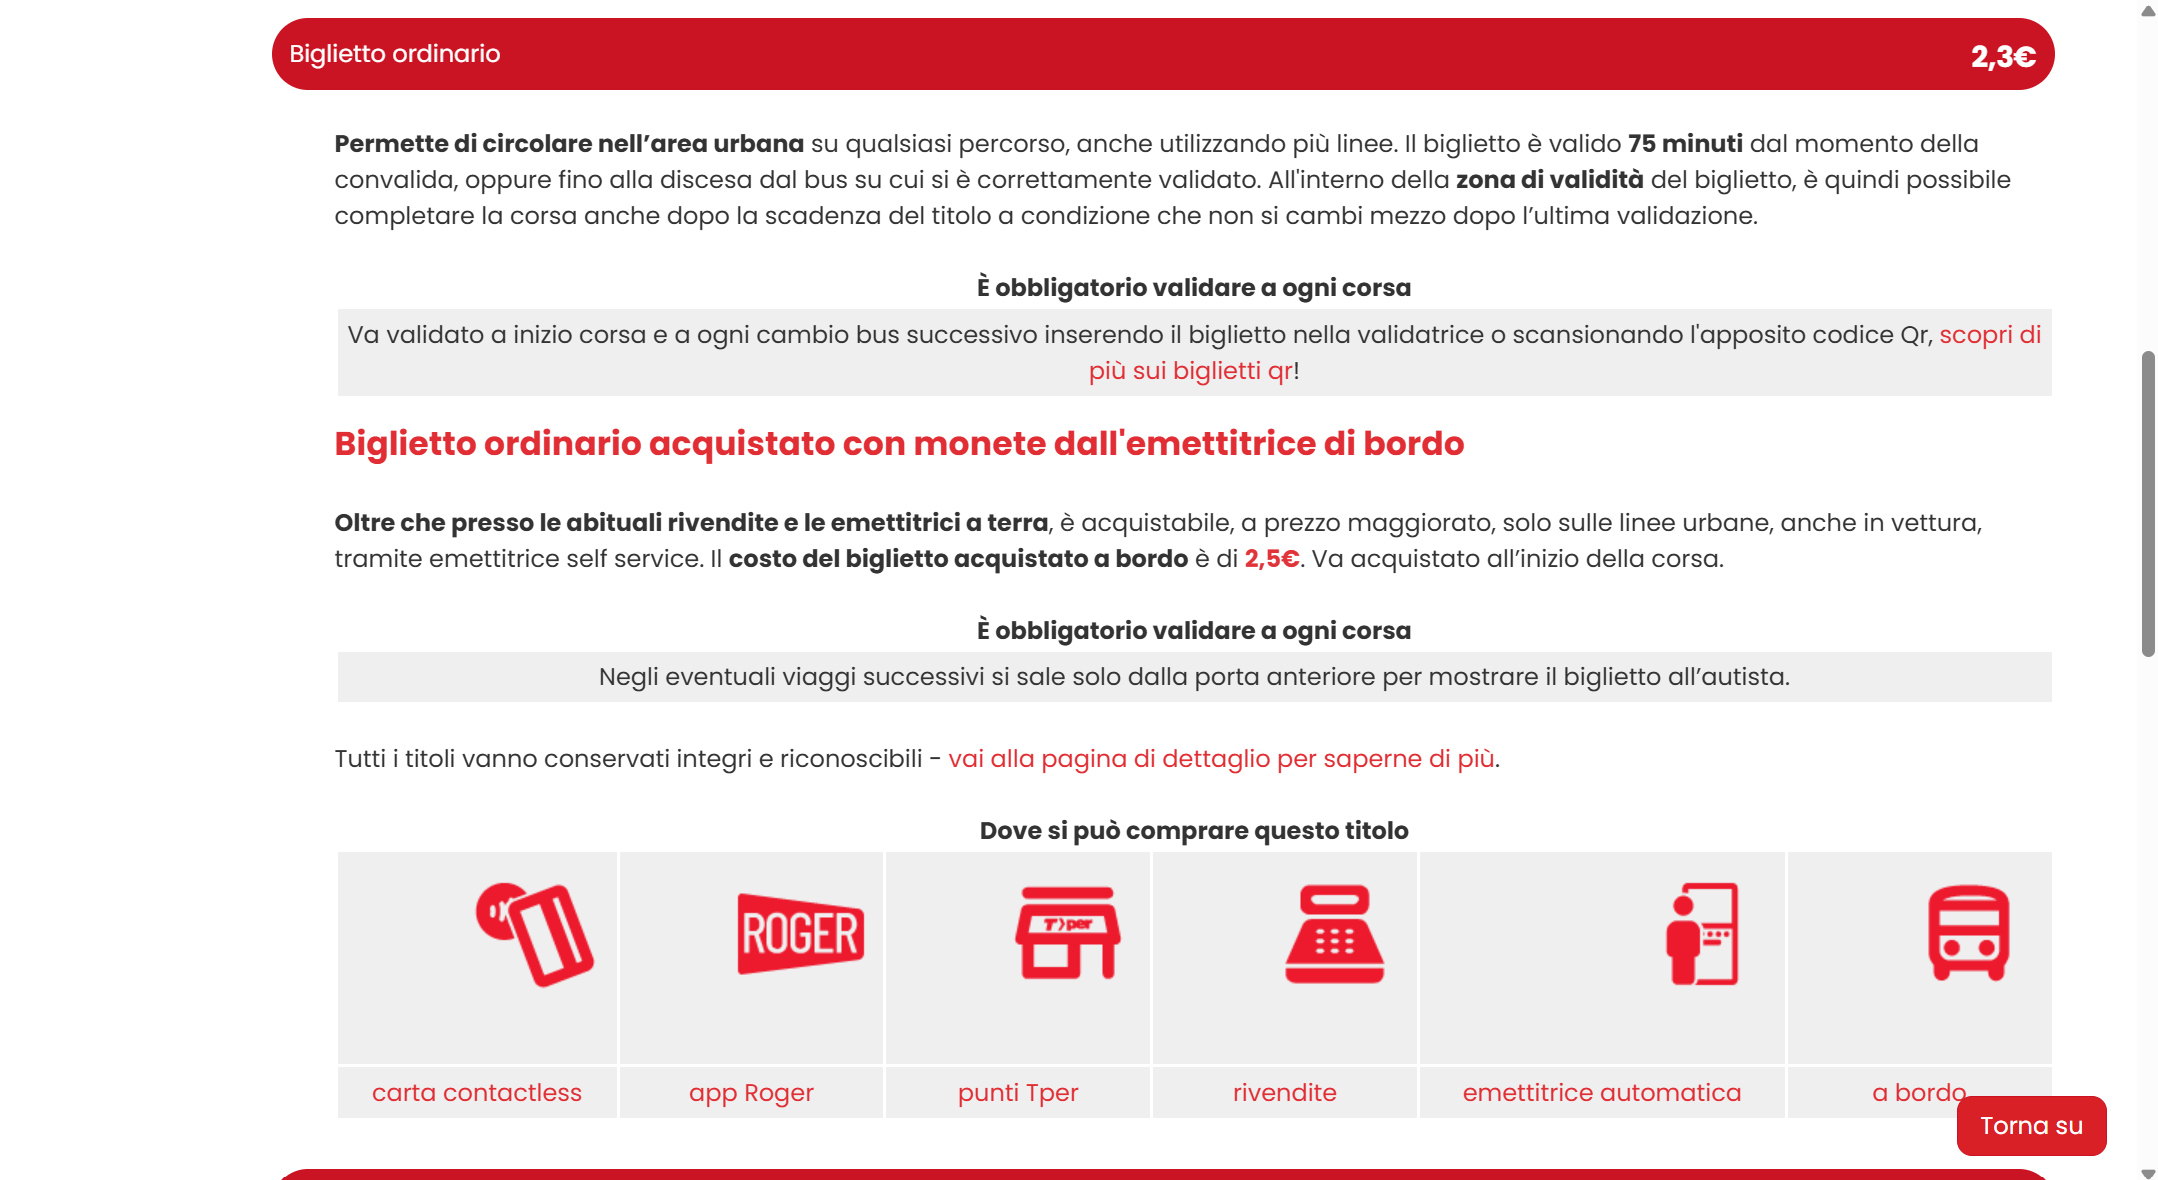
\includegraphics[width=0.332\textwidth]{Tper sito originale/Biglietti.png}\hfill
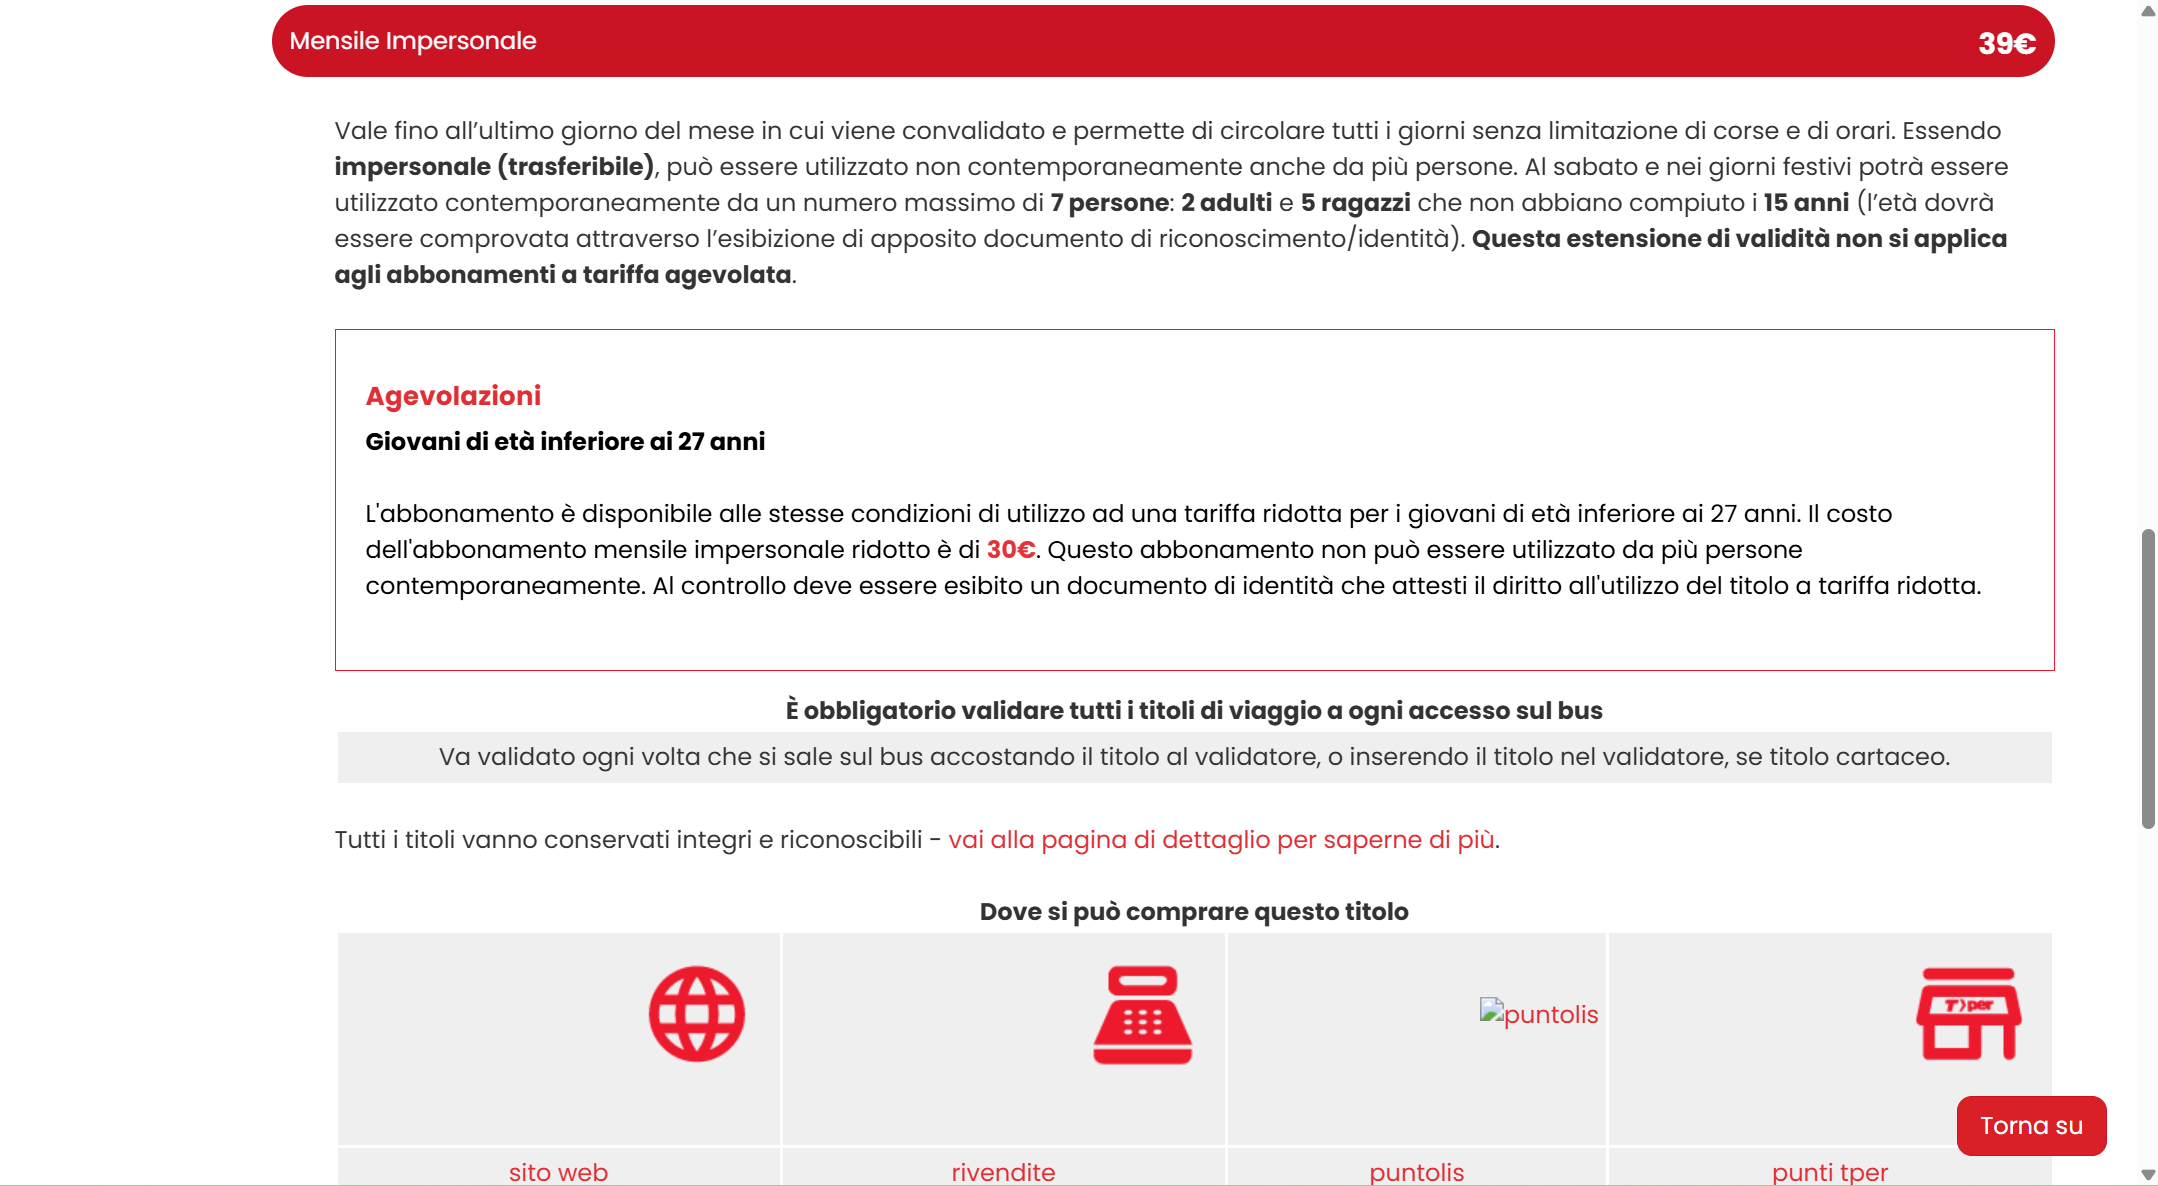
\includegraphics[width=0.332\textwidth]{Tper sito originale/Abbonamenti.png}\hfill
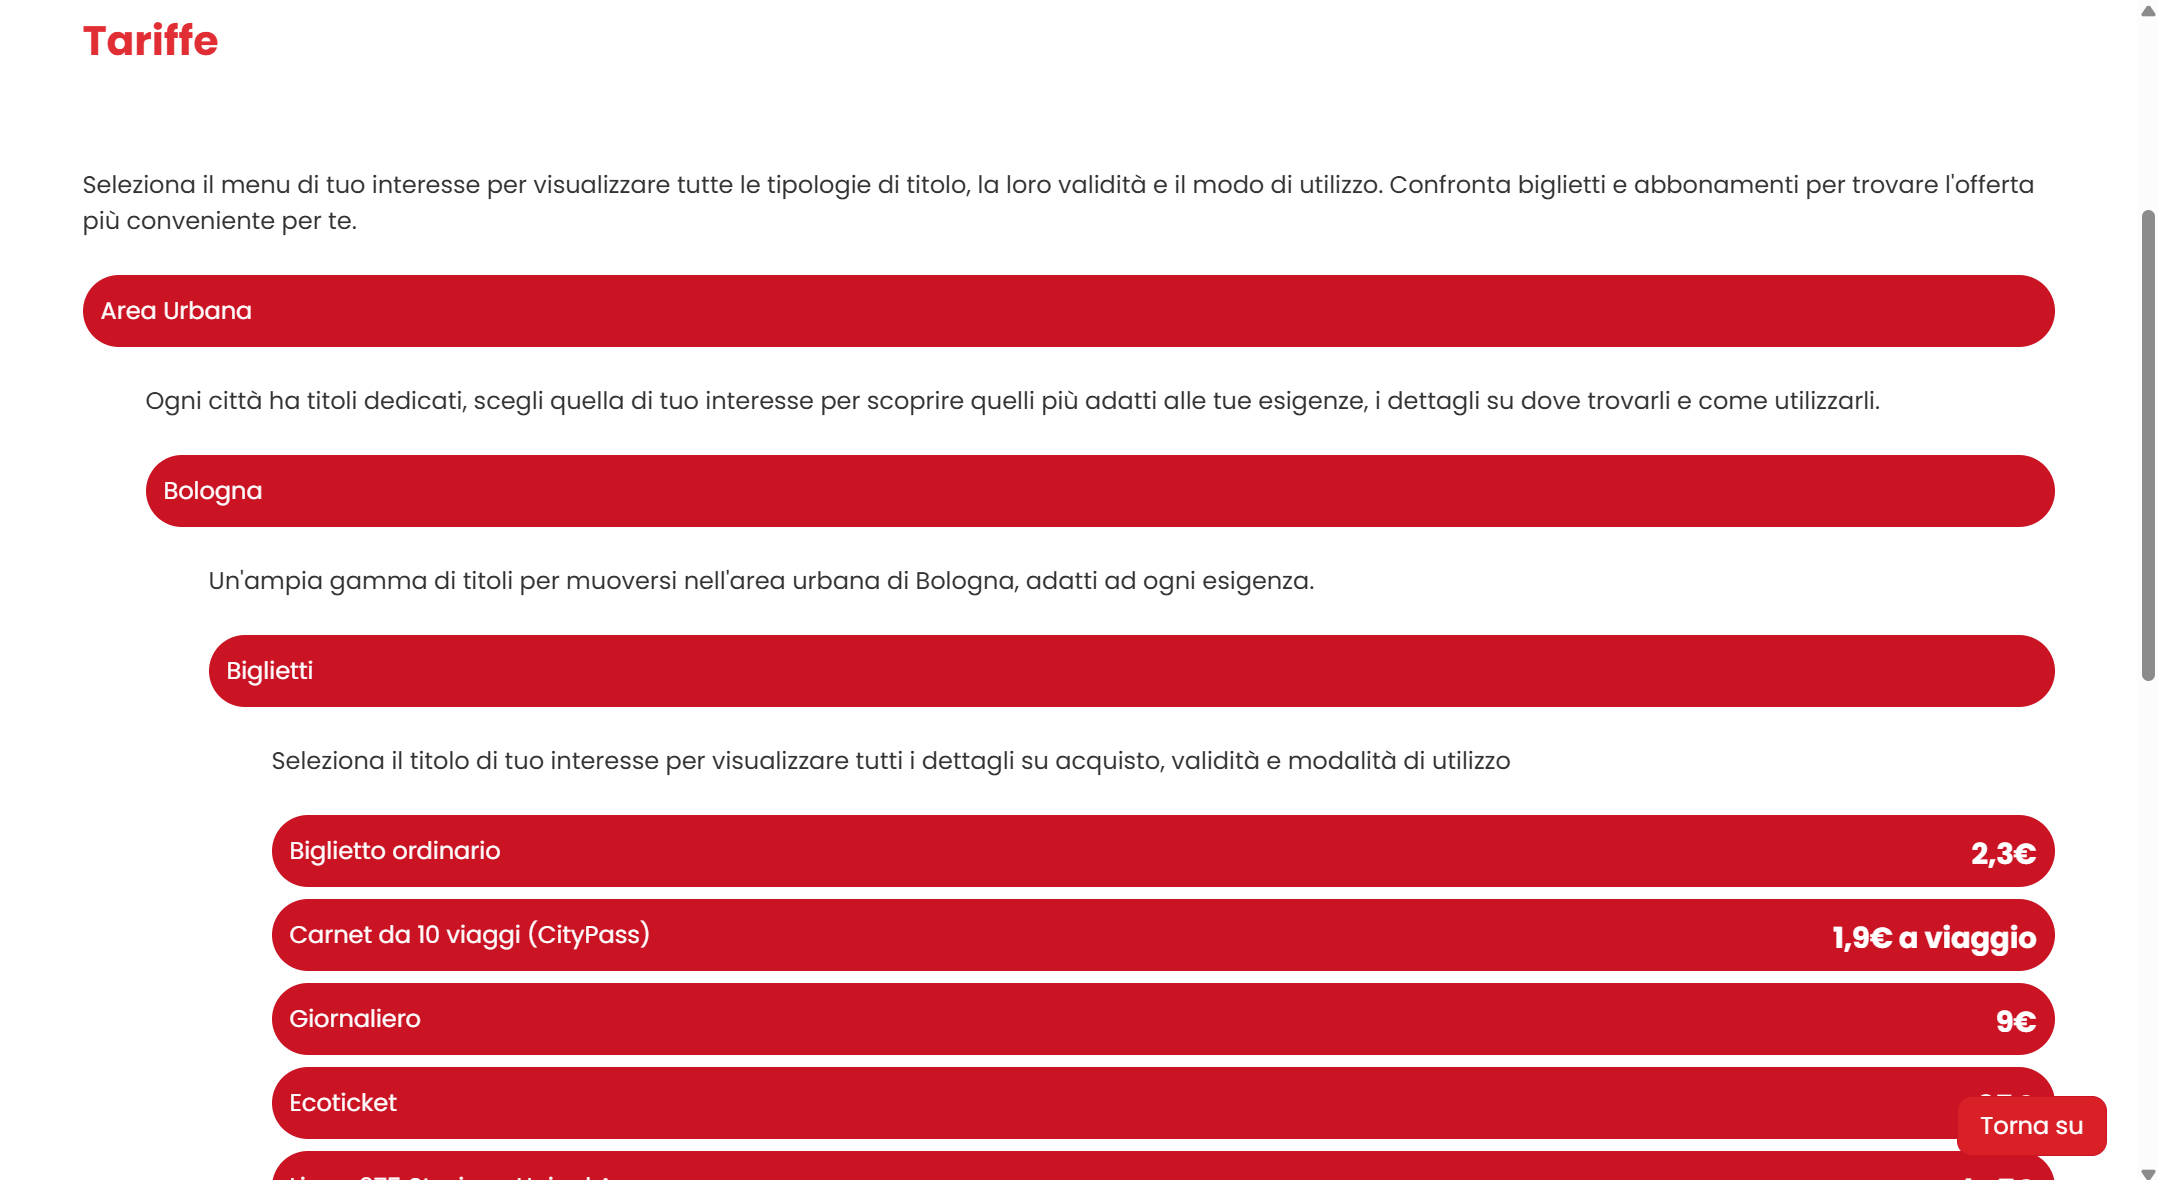
\includegraphics[width=0.332\textwidth]{Tper sito originale/Tariffe.png}\\[2pt]
{\small\textit{Tickets \hspace{3.7cm} Subscriptions \hspace{3.3cm} Tariffs}}\\[2pt]
{\footnotesize A single page with 3 sections: duplicated content, buried channels, corporate terminology}

\vspace{0.5cm}

\textbf{After --- tper 2.0 Redesign}\\[4pt]
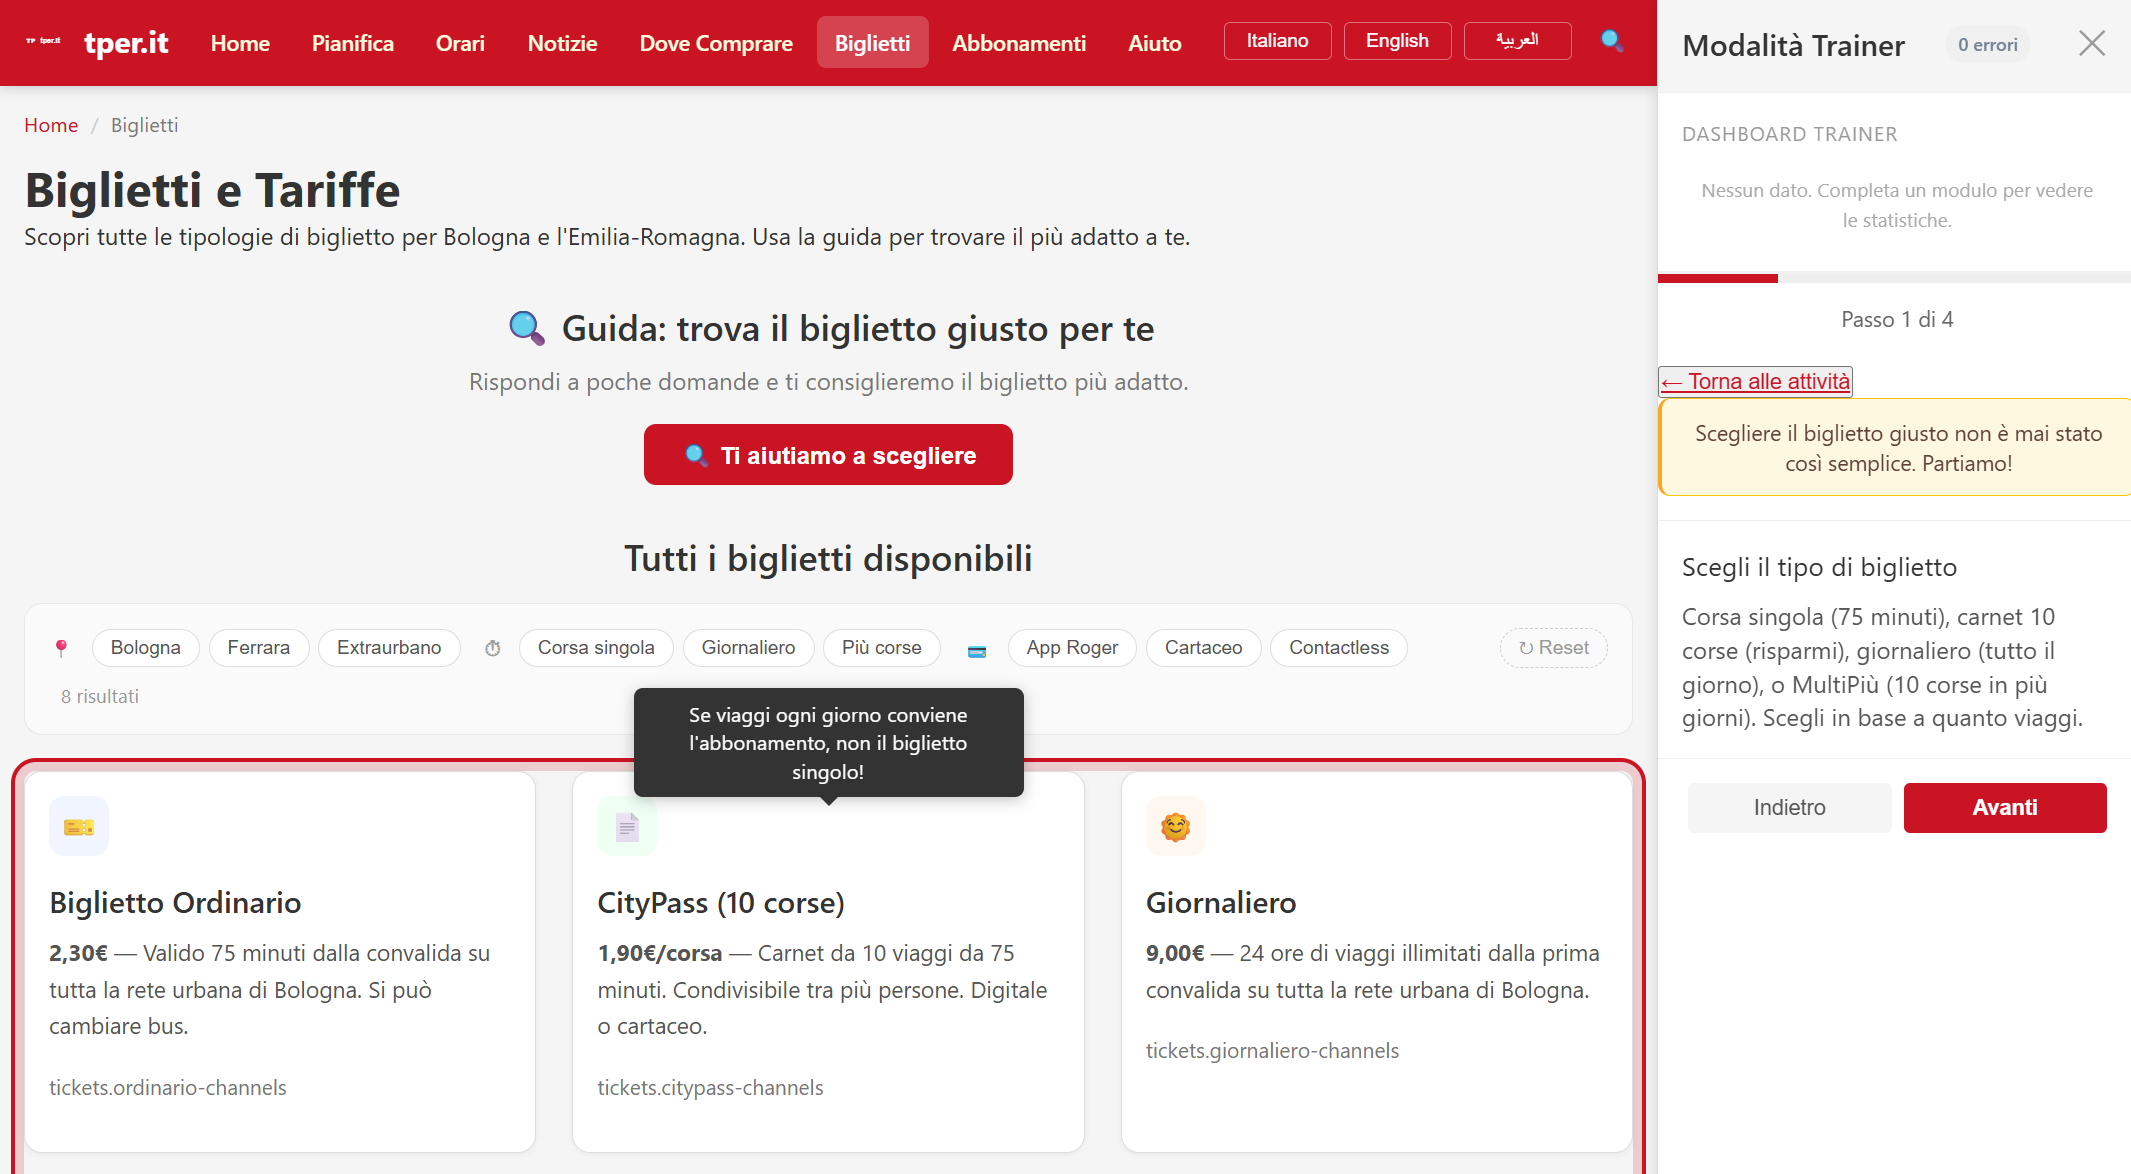
\includegraphics[width=0.332\textwidth]{Redesign Tper 2.0/Biglietti.png}\hfill
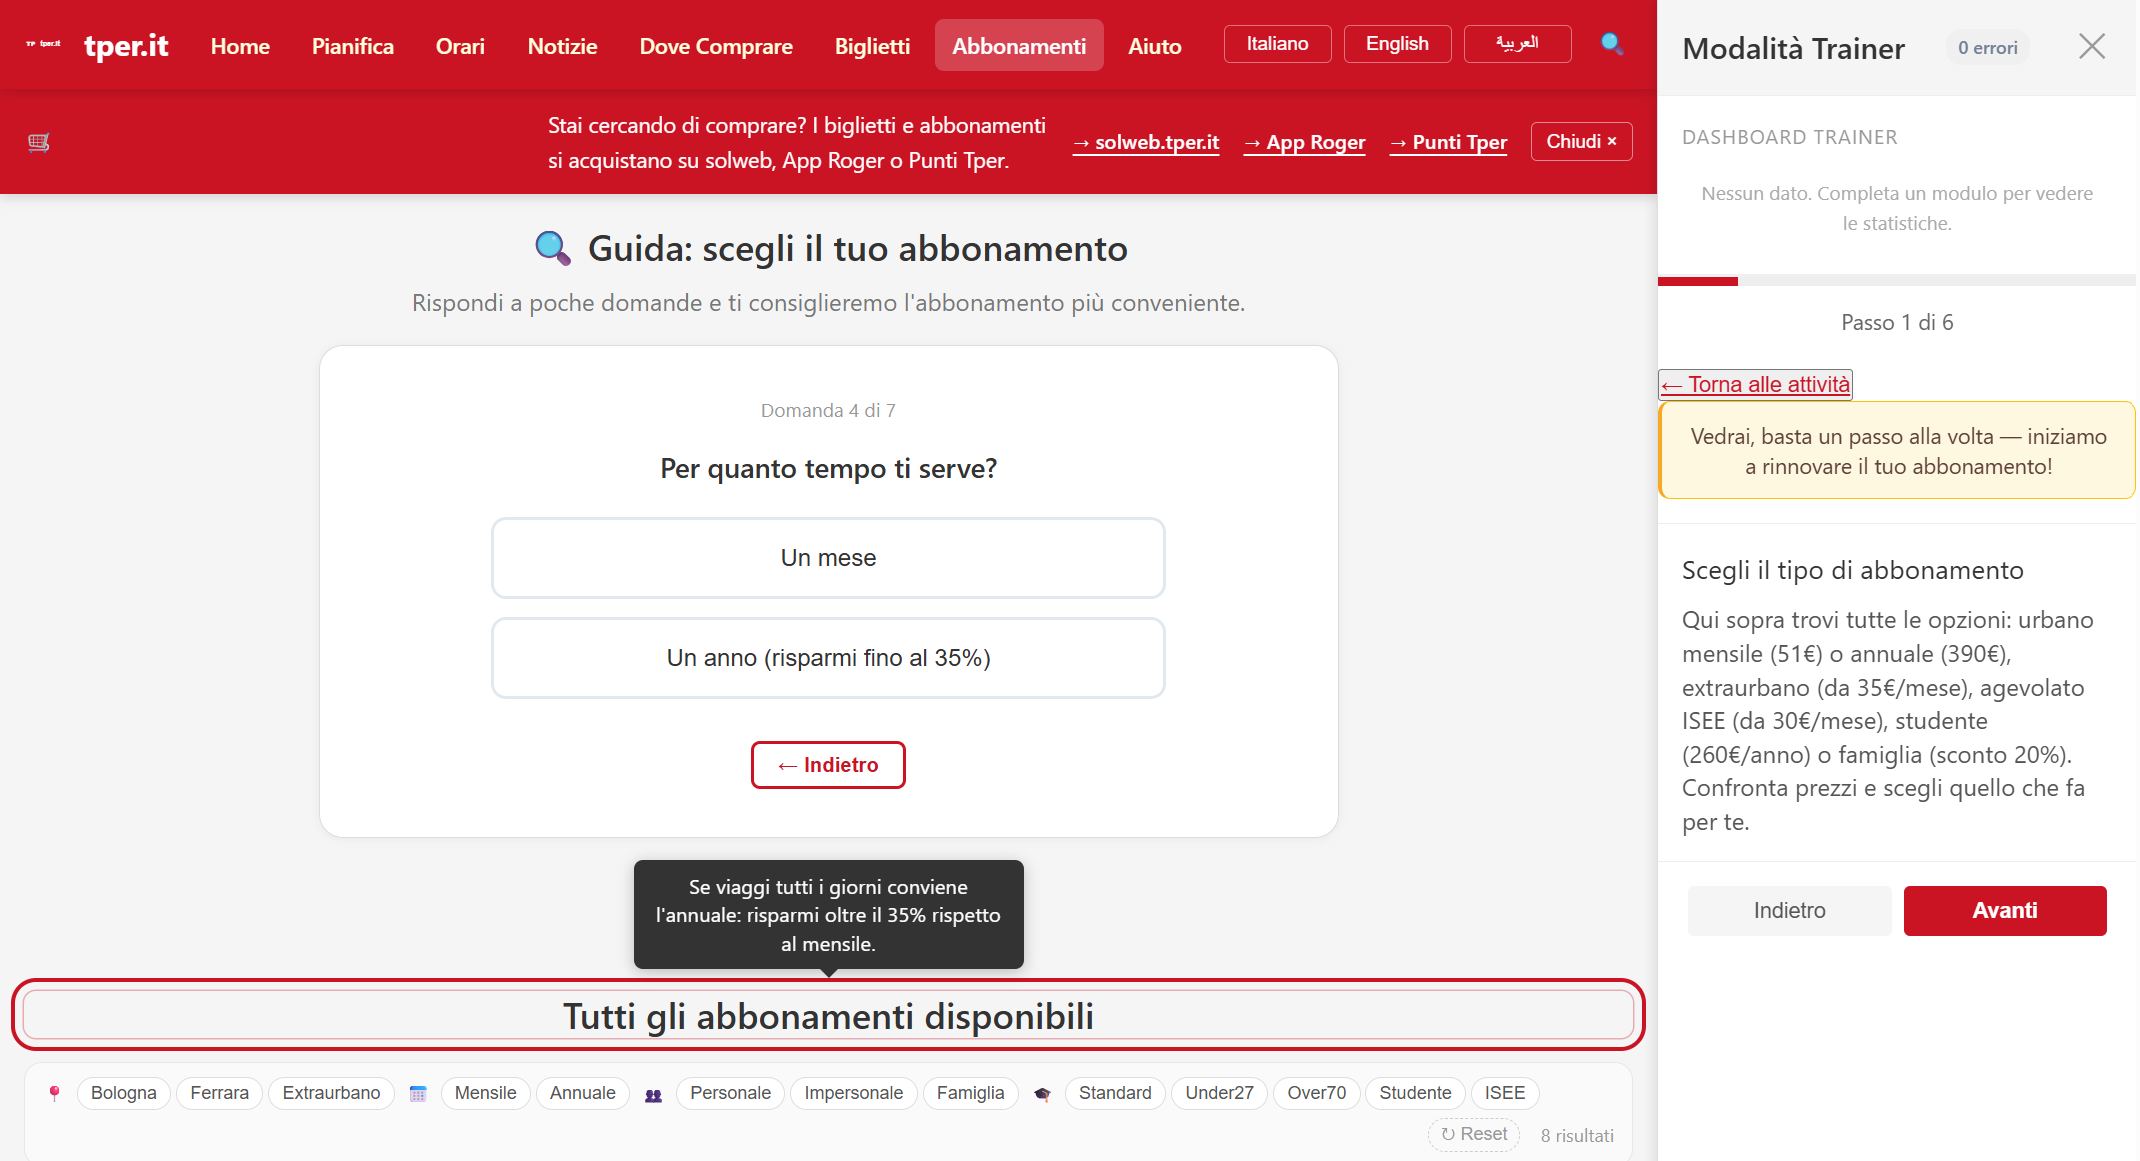
\includegraphics[width=0.332\textwidth]{Redesign Tper 2.0/Abbonamenti.png}\hfill
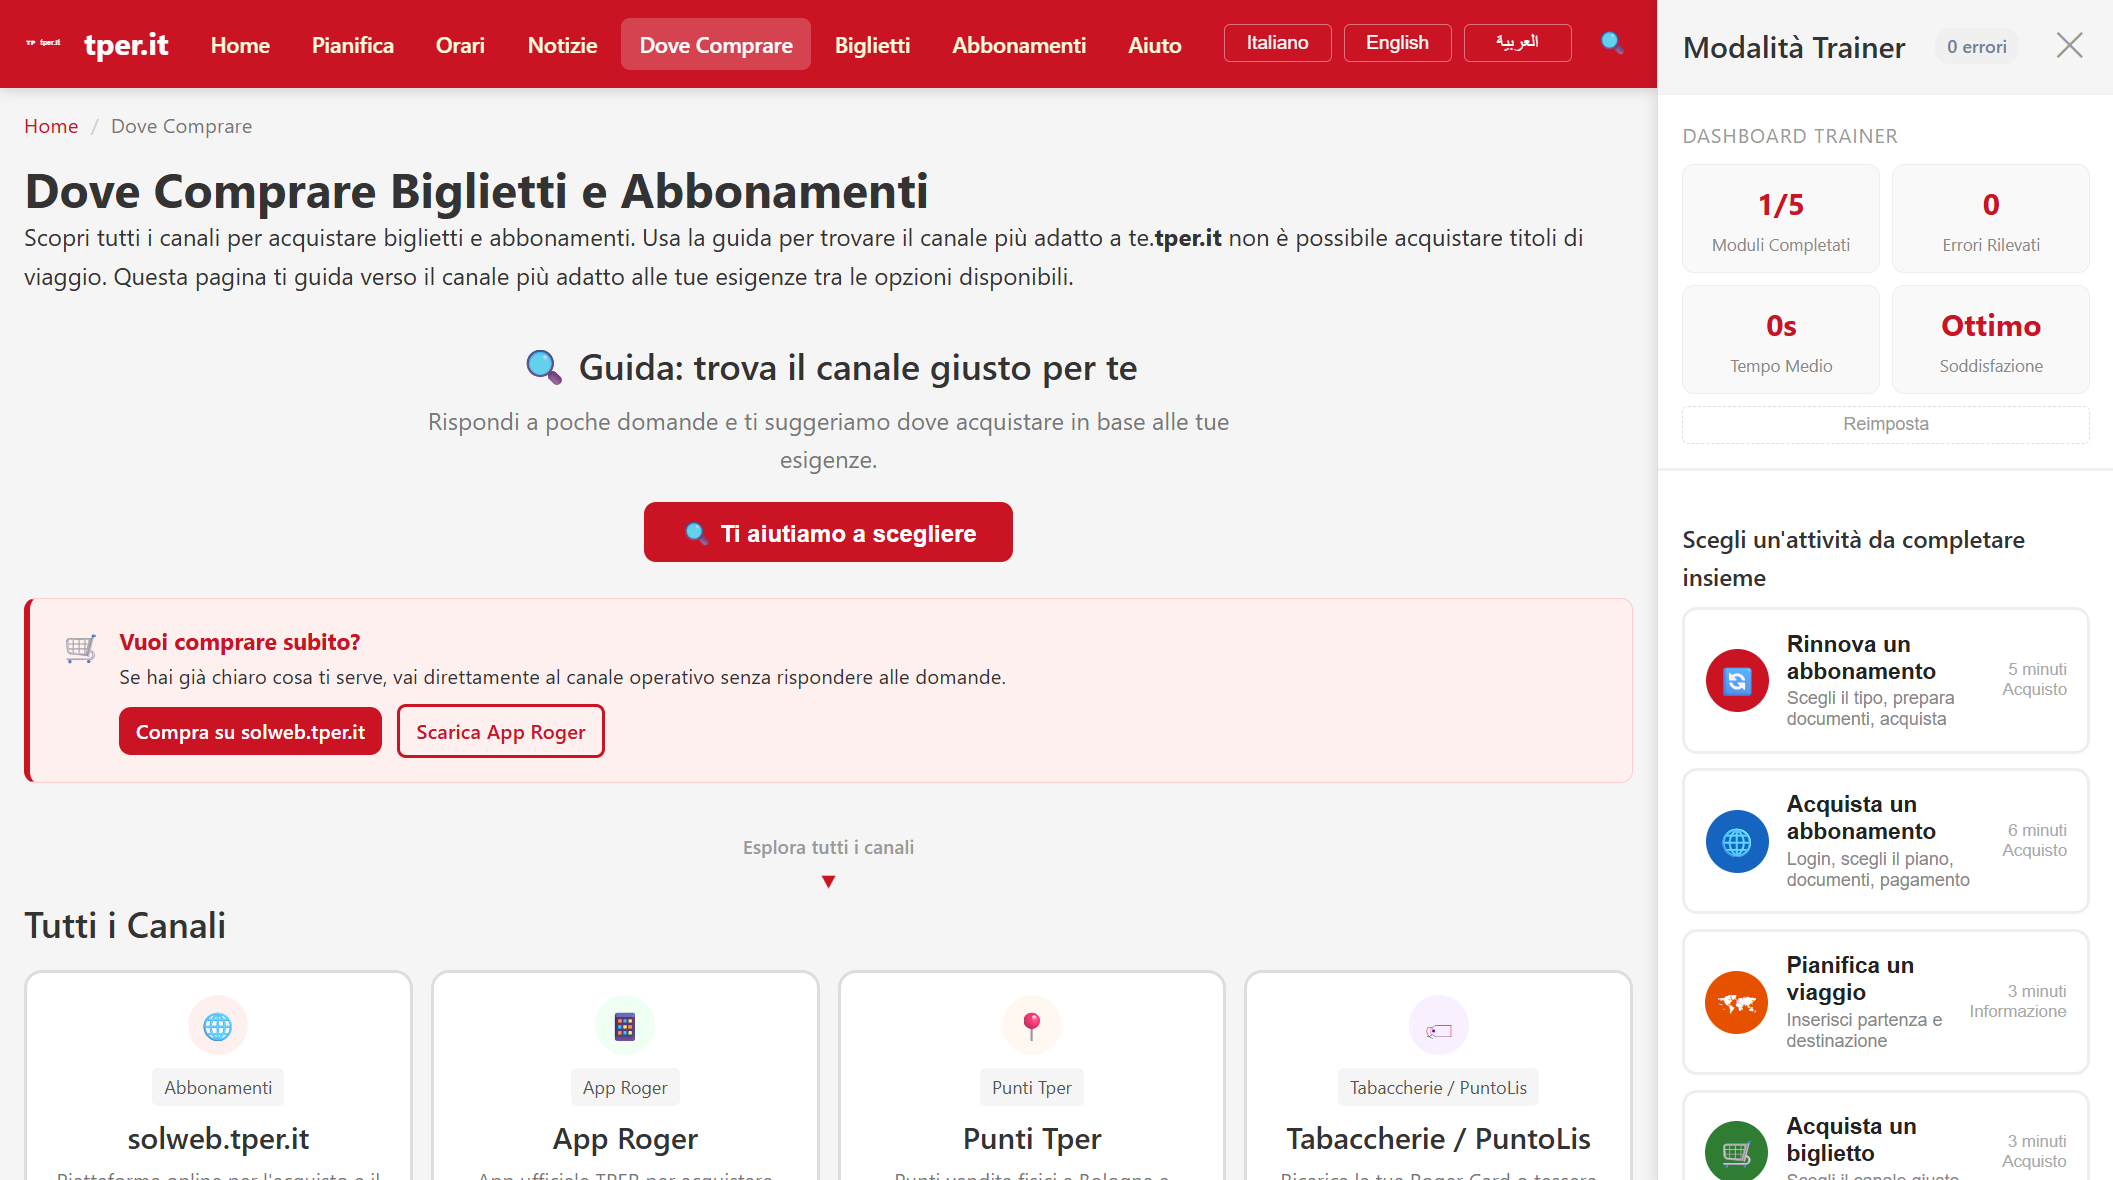
\includegraphics[width=0.332\textwidth]{Redesign Tper 2.0/Dove Comprare.png}\\[2pt]
{\small\textit{Tickets \hspace{3.7cm} Subscriptions \hspace{2.8cm} Where to Buy}}\\[2pt]
{\footnotesize 3 specialised pages: each page has a unique task, tariffs integrated into products}

\caption{3v3 Comparison --- Information Architecture Restructuring}
\label{fig:comparison-ia-3v3}
\end{figure}

\begin{table}[H]
\centering
\small
\renewcommand{\arraystretch}{1.4}
\begin{tabular}{|p{0.5cm}|p{7cm}|p{7cm}|}
\hline
& \textbf{Before (Original)} & \textbf{After (Redesign 2.0)} \\ \hline
\cellcolor{primaryColor!15} &
\textit{A single page, 3 overlapping sections} &
\textit{3 specialised pages} \\ \hline

\raisebox{0.5cm}{\rotatebox{90}{\textbf{Structure}}} &
A single page with 3 overlapping sections and blurred boundaries. Tickets and Subscriptions both contain references to tariffs and channels. The Tariffs section is redundant. 3+ level navigation to reach the channel guide (D2). &
3 pages with clear and distinct responsibilities. Each page has a single task. No duplication. Direct access to each section from the main navigation (max 1 click). Tariffs are displayed in the product context (R2). \\ \hline

\raisebox{0.5cm}{\rotatebox{90}{\textbf{Tickets}}} &
Lists ticket types, but also includes sales channel information and tariff references. The user cannot tell if this is the right page to decide what to buy or where to buy it (D2, D3). &
Page focused exclusively on tickets. 5-question wizard (zone, frequency, duration, app, travel companion). Filter pills for zone/validity/channel with counter and reset. Info banner: ``tper.it is an informational website''. \\ \hline

\raisebox{0.5cm}{\rotatebox{90}{\textbf{Subscriptions}}} &
Lists subscription plans with corporate terminology (MiMuovo, SaltaSu, Prontobus). Includes channels and tariffs. No selection guidance: the user must read all options and deduce which one suits them (UR-05). &
Page focused exclusively on subscriptions. 7-question wizard (action, impersonal?, zone, duration, holder, concession, channel). 4-group filter. Accordion ``How to Purchase or Renew''. Callout to check discount eligibility (R9). \\ \hline

\raisebox{0.5cm}{\rotatebox{90}{\textbf{Channels / Tariffs}}} &
\textbf{Channels}: ``Sales Network'' buried under Tickets and Subscriptions, reachable in 3 clicks. \textbf{Tariffs}: separate pricing section on the same page, disconnected from the usage context --- the user must remember the price while navigating elsewhere to decide (D3). &
\textbf{Where to Buy}: standalone, prominent section in the main navigation. 3-question wizard $\rightarrow$ recommended channel with icon, description, and direct link. Comparison table 5 channels $\times$ 7 operations. \textbf{Tariffs}: integrated into Tickets and Subscriptions --- visible at the moment of decision (R2, R4). \\ \hline

\raisebox{0.5cm}{\rotatebox{90}{\textbf{Impact}}} &
6/20 tasks completed (30\%). Average SUS 37.5/100. Maria B. (79 yrs): 0/5 tasks, 652\,s avg, 13 errors per task. &
Phase D data: Laura P. 4/5 tasks (80\%), SUS 72.5 (+35 points). T4 (concessions): from 195\,s and 7 errors to 57\,s and 0 errors. Separating concerns eliminated the confusion between ``what to buy'' and ``where to buy''. \\ \hline
\end{tabular}
\caption{IA Restructuring: Tickets, Subscriptions, and Channels}
\label{tab:comparison-ia-3v3}
\end{table}

\vspace{0.3cm}



% ============================================================
% COMPARISON 4: CONCESSIONS AND DISCOUNTS
% ============================================================
\section{Concessions and Discounts}
\label{sec:comparison-agevolazioni}

\textbf{UR-05 $\rightarrow$ R9+R11} --- User does not know which discounts they are entitled to $\rightarrow$ 4-question wizard + ISEE tooltip. David Carter pays 50\euro/month for 3 months before discovering he is entitled to 30\euro.

\begin{figure}[H]
\centering
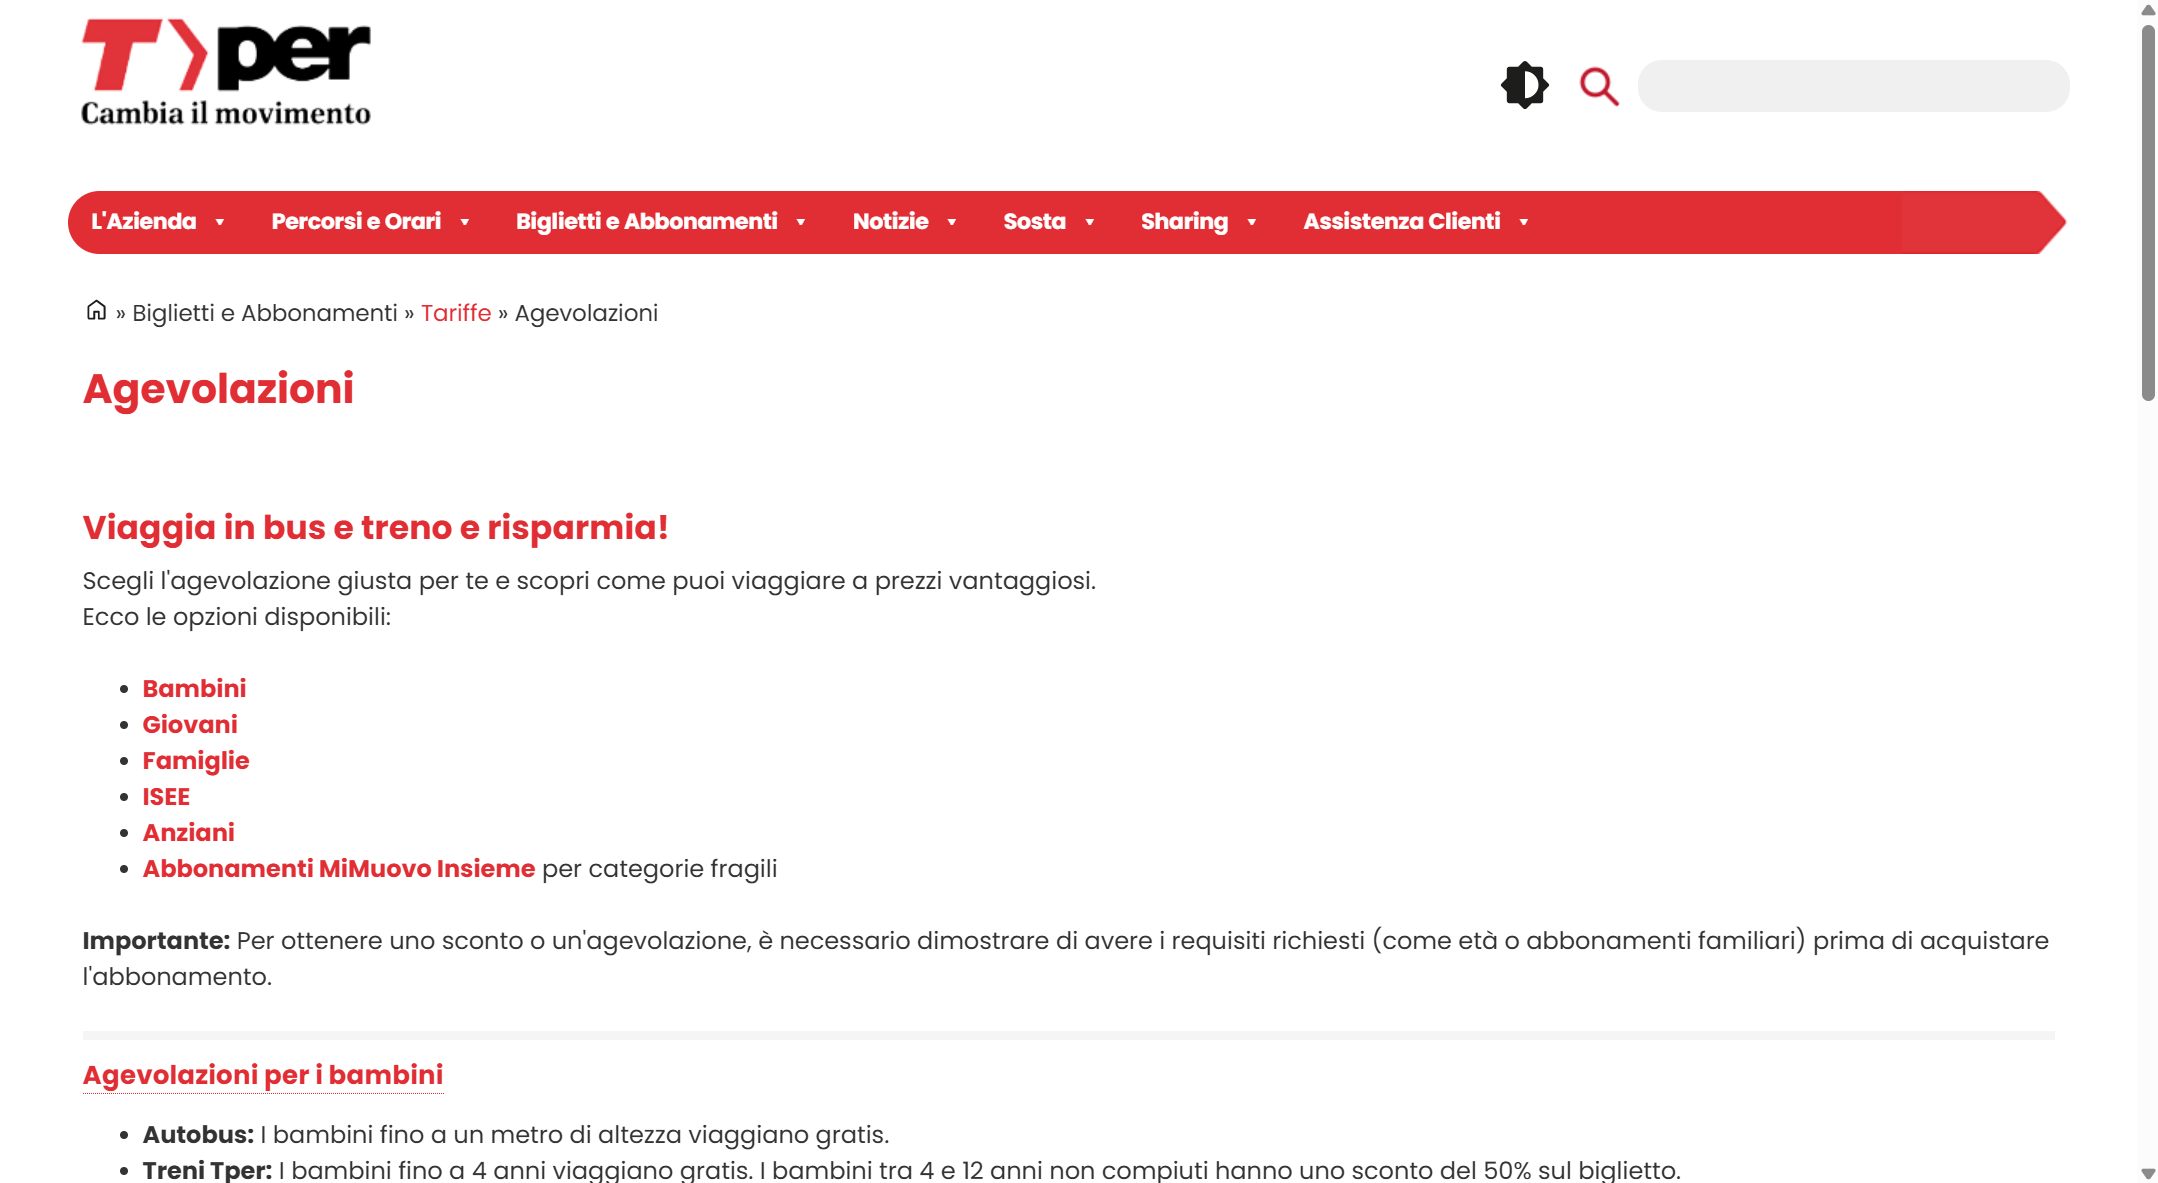
\includegraphics[width=0.85\textwidth]{Tper sito originale/Agevolazioni.png}
\par\small\textit{Before: original concessions page --- bureaucratic language, no guidance}
\vspace{0.4cm}
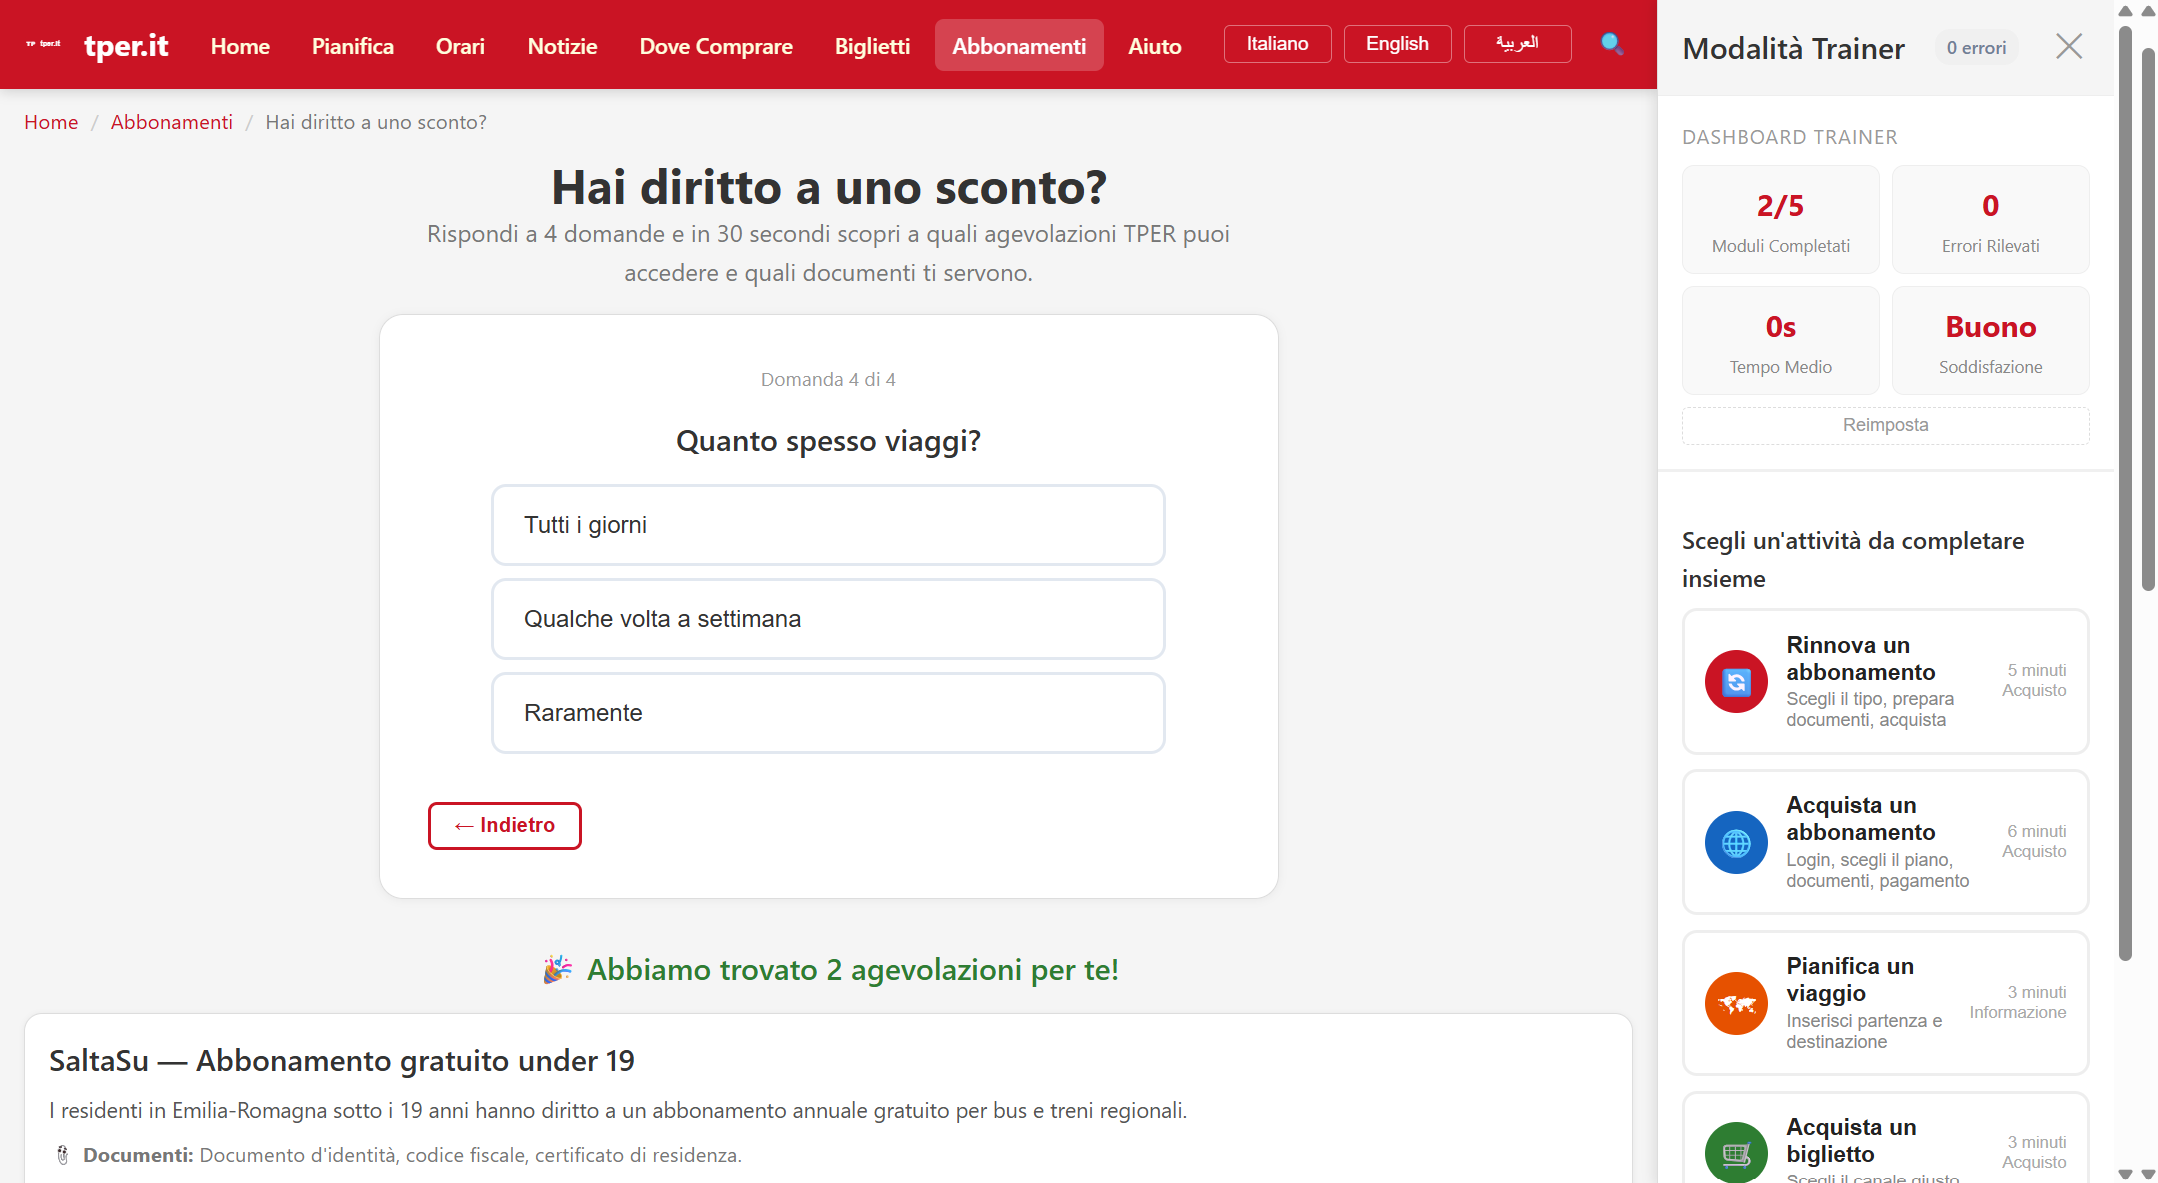
\includegraphics[width=0.85\textwidth]{Redesign Tper 2.0/Agevolazioni.png}
\par\small\textit{After: concessions wizard 2.0 --- 4 questions, personalised results, ISEE tooltip}
\caption{Concessions and Discounts}
\label{fig:comparison-agevolazioni}
\end{figure}

\begin{table}[H]
\centering
\small
\renewcommand{\arraystretch}{1.4}
\begin{tabular}{|p{0.5cm}|p{7cm}|p{7cm}|}
\hline
& \textbf{Before} & \textbf{After} \\ \hline
\cellcolor{primaryColor!15} &
\textit{Original concessions section} &
\textit{Concessions wizard in tper 2.0} \\ \hline

\raisebox{0.5cm}{\rotatebox{90}{\textbf{Access}}} &
Section buried 3+ levels deep in the navigation. Only reachable through ``Subscriptions'' $\rightarrow$ ``Carta Agevolata''. No direct path from the homepage (D2, UR-05). &
\textbf{Dedicated ``Am I entitled to a discount?'' path} visible from the homepage (``Discover Subscriptions'' card) and from the Subscriptions page with a prominent callout ``Find out in 30 seconds which discounts you can access''. Breadcrumb: Home $\rightarrow$ Subscriptions $\rightarrow$ Concessions (R2, R9). \\ \hline

\raisebox{0.5cm}{\rotatebox{90}{\textbf{Language}}} &
Bureaucratic register: ``ISEE'', ``DSU'', ``Carta Agevolata'', ``brackets'', ``resolutions''. No explanation of terms. For a foreign user (David Carter, language competence 2/5), terms remain incomprehensible even with Google Translate (UR-05, Use Case \#2). &
\textbf{Citizen-friendly language} with explanatory tooltips. On hover over ``ISEE'' it shows ``Indicatore della Situazione Economica Equivalente. Certifies the household income. Obtainable free of charge at CAF or online at INPS.'' Same approach for ``DSU'' and ``Carta Agevolata''. Available in IT/EN/AR (R9, R12). \\ \hline

\raisebox{0.5cm}{\rotatebox{90}{\textbf{Wizard}}} &
\textbf{Absent.} The user must read pages of resolutions and brackets to discover if they are entitled to a discount. No interactive guidance. David Carter's test shows 15 minutes of attempts followed by abandonment (Use Case \#2). &
\textbf{4-question wizard}: (1) How old are you? (2) Do you have an ISEE? (3) How often do you use public transport? (4) Who is the subscription for? Each answer filters available discounts in real time. Result: ``We found X discounts for you!'' with name, description, required documents, and direct link (RF-35, R9). \\ \hline

\raisebox{0.5cm}{\rotatebox{90}{\textbf{Documents}}} &
No preventive checklist. Required documents (ISEE, DSU, passport photo, ID) mentioned on separate bureaucratic pages. The user arrives at the counter without the right documents (Roberto, Use Case \#1). &
\textbf{Integrated document checklist} in the wizard results: each discount shows exactly which documents are needed, with tooltips on where to obtain them. Visual document reproduction (e.g. ``ISEE --- first page'' with yellow highlight of the value). ``View Subscriptions'' link to proceed with purchase (R11). \\ \hline

\raisebox{0.5cm}{\rotatebox{90}{\textbf{Impact}}} &
David Carter (Phase A): 3 months paying 50\euro/month instead of 30\euro. Roberto: arrives at the counter without documents and postpones. Average SUS 37.5/100. &
Laura P. (Phase D, T4): from 195\,s and 7 errors to 57\,s and 0 errors. Concessions wizard completed in 30 seconds. ISEE tooltip used spontaneously. SUS 72.5 (+35 points). \\ \hline
\end{tabular}
\caption{Concessions and Discounts}
\label{tab:comparison-agevolazioni}
\end{table}

\vspace{0.3cm}

% ============================================================
% COMPARISON 5: TRIP PLANNING
% ============================================================
\section{Trip Planning}
\label{sec:comparison-planning}

\textbf{D2 $\rightarrow$ R1+R2} --- Route planner on a separate page, reachable via the ``Routes and Timetables'' link on the homepage (1 click), but with no search fields visible directly on the homepage $\rightarrow$ Hero search + dedicated page. Maria: 724\,s, 16 errors, 19 backtracks on T2 (Phase A).

\begin{figure}[H]
\centering
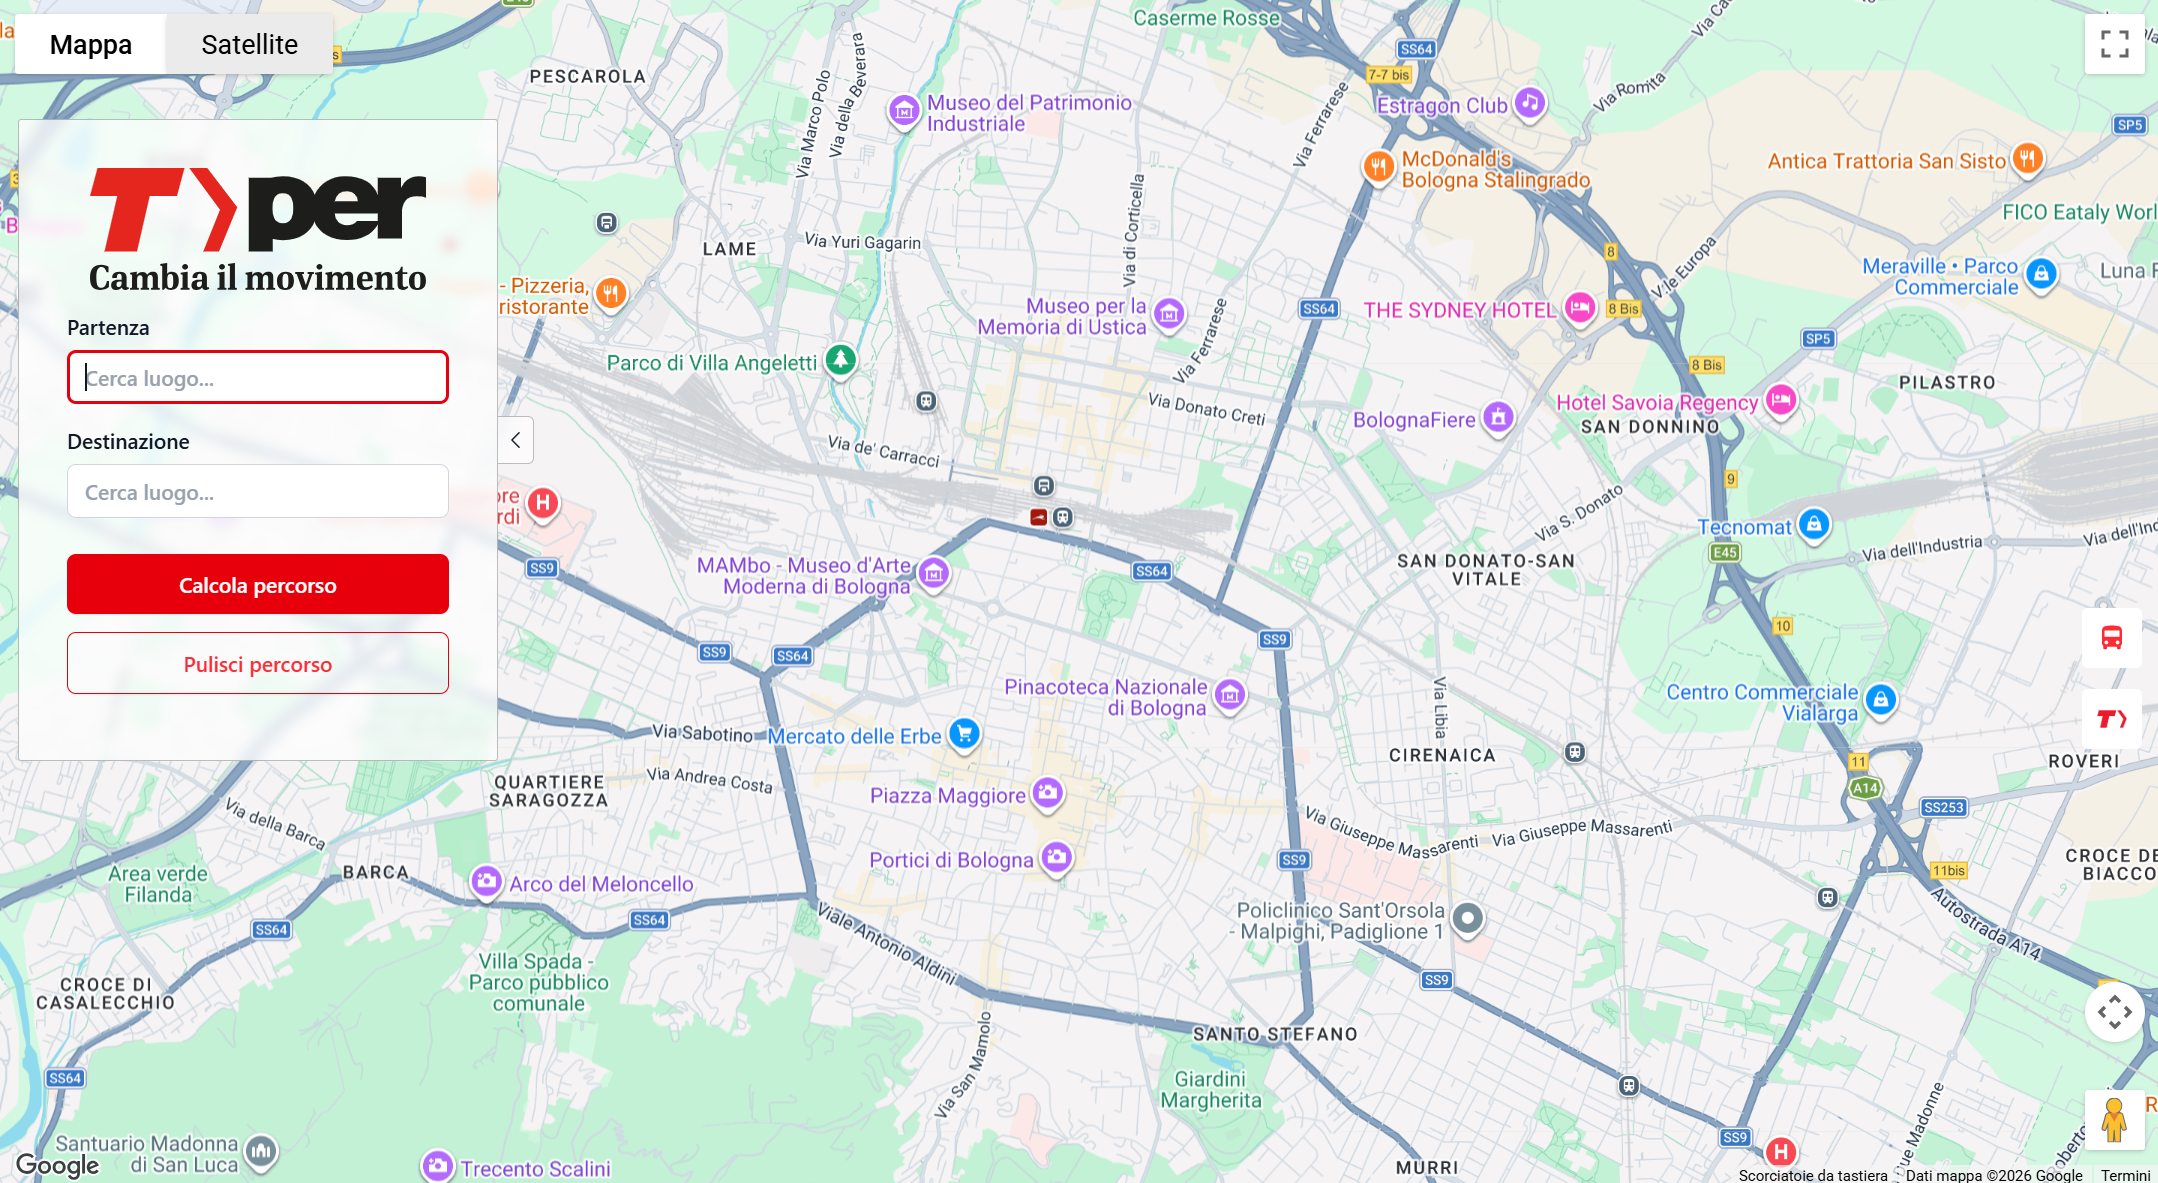
\includegraphics[width=0.85\textwidth]{Tper sito originale/Percorsi.png}
\par\small\textit{Before: original planner --- reachable from the homepage via ``Routes and Timetables'' (homepage link) $\rightarrow$ ``Calculate your route''}
\vspace{0.4cm}
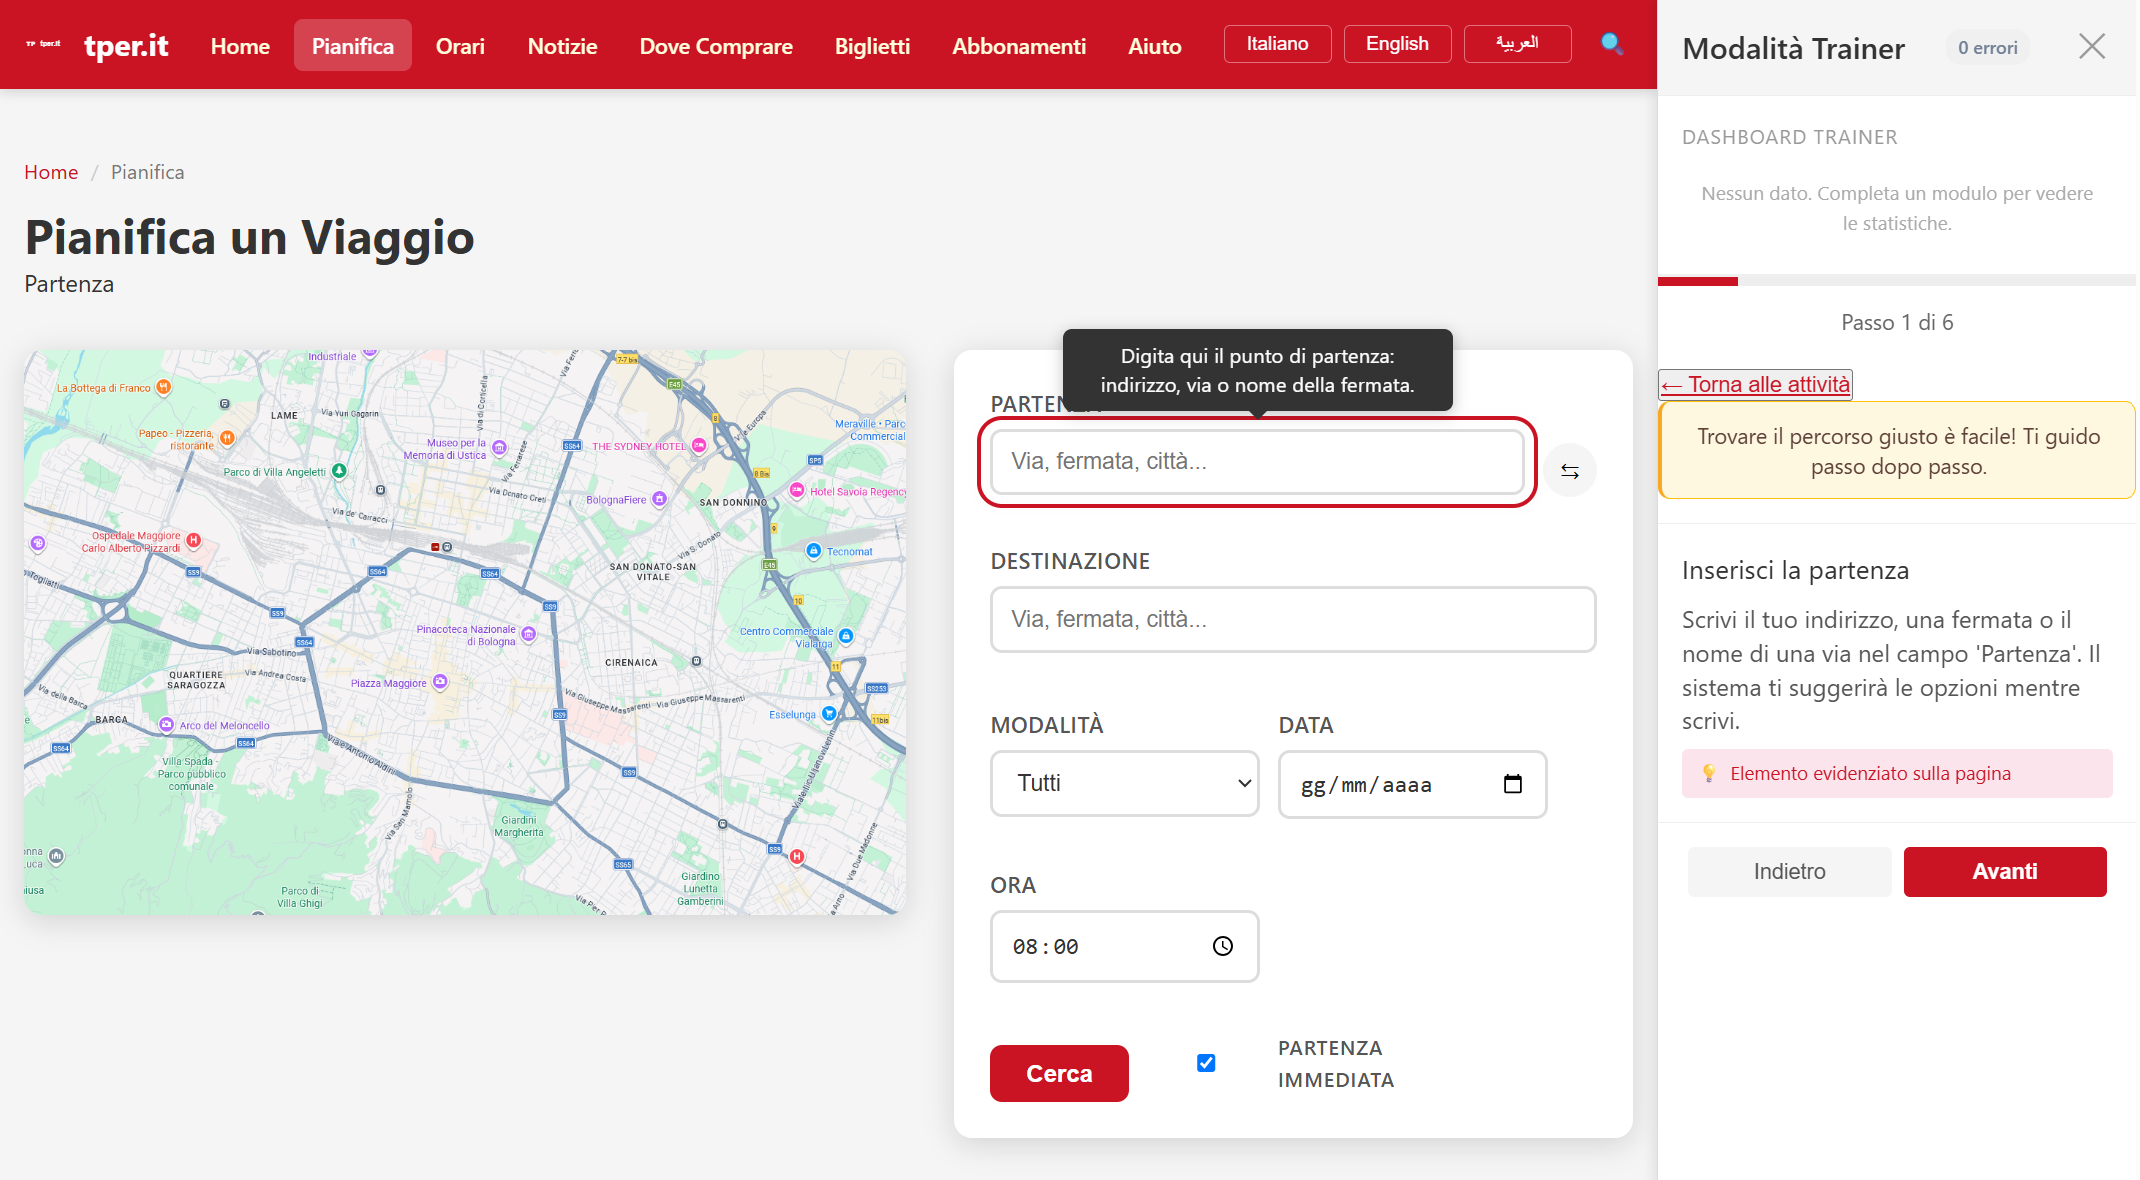
\includegraphics[width=0.85\textwidth]{Redesign Tper 2.0/Percorsi.png}
\par\small\textit{After: trip planner 2.0 --- hero search on homepage + dedicated page with map and form}
\caption{Trip Planning}
\label{fig:comparison-planning}
\end{figure}

\begin{table}[H]
\centering
\small
\renewcommand{\arraystretch}{1.4}
\begin{tabular}{|p{0.5cm}|p{7cm}|p{7cm}|}
\hline
& \textbf{Before} & \textbf{After} \\ \hline
\cellcolor{primaryColor!15} &
\textit{Original \texttt{tper.it} route planner} &
\textit{Trip planning in tper 2.0} \\ \hline

\raisebox{0.5cm}{\rotatebox{90}{\textbf{Access}}} &
``Routes and Timetables'' link visible on the homepage (1 click), leading to the planner page. No search fields visible directly on the homepage. The user must recognise the corporate label ``Routes and Timetables'' to start the task (D3). &
\textbf{Hero search on homepage}: ``From'' and ``To'' fields visible with no clicks needed. ``Plan'' section in main navigation (1 click). ``Plan'' card in the ``What do you want to do?'' grid with distinctive icon (R1, R2). \\ \hline

\raisebox{0.5cm}{\rotatebox{90}{\textbf{Form}}} &
Text search form with no suggestions. Single combined from/to field. No transport mode filter. No interactive map. &
\textbf{Full form}: separate from/to fields with swap button. Transport modes (bus/train/bike/walk). Date and time with ``Depart now'' checkbox. Interactive Bologna map alongside (click to enlarge). Autocomplete on fields (R1). \\ \hline

\raisebox{0.5cm}{\rotatebox{90}{\textbf{Results}}} &
Text list of results without timetables or duration. No price indication. No link to purchase channel. The user must take notes and search elsewhere for how to buy the ticket (UR-01, UR-03). &
\textbf{Structured results} with timetables, duration, and informative price for each option. ``Where to Buy'' link integrated in each result. Map/list toggle. Informational banner: ``On tper.it you cannot purchase --- find out how and where to buy'' (R1, R6). \\ \hline

\raisebox{0.5cm}{\rotatebox{90}{\textbf{Impact}}} &
Maria B. (Phase A): 724\,s, 16 errors, 19 backtracks. Cannot find the planner and gives up after 12 minutes. Average SUS 37.5/100. &
Laura P. (Phase D, T2): 115\,s, 1 error, 0 backtracks. ``Plan'' card recognised immediately. Hero search used without hesitation. SUS 72.5 (+35 points). \\ \hline
\end{tabular}
\caption{Trip Planning}
\label{tab:comparison-planning}
\end{table}

\vspace{0.3cm}

% ============================================================
% COMPARISON 6: TRAINER MODE AND SUPPORT
% ============================================================
\section{Trainer Mode and Support}
\label{sec:comparison-trainer}

\textbf{R5 $\rightarrow$ R4+R5+R6} --- No trainer $\rightarrow$ Sidebar 22 pages, 5 modules, operator script. Maria 0/5 tasks, SUS 27.5.

\begin{figure}[H]
\centering
\fcolorbox{borderColor}{backgroundColor}{%
\begin{minipage}{0.78\textwidth}
\centering
\vspace{1.5cm}
{\large\sffamily\textcolor{secondaryColor}{No Trainer Mode}}\\[4pt]
\small\textit{The original site offered no assisted mode whatsoever.}
\vspace{1.5cm}
\end{minipage}}
\par\small\textit{Before: no trainer mode --- only telephone help desk}
\vspace{0.4cm}
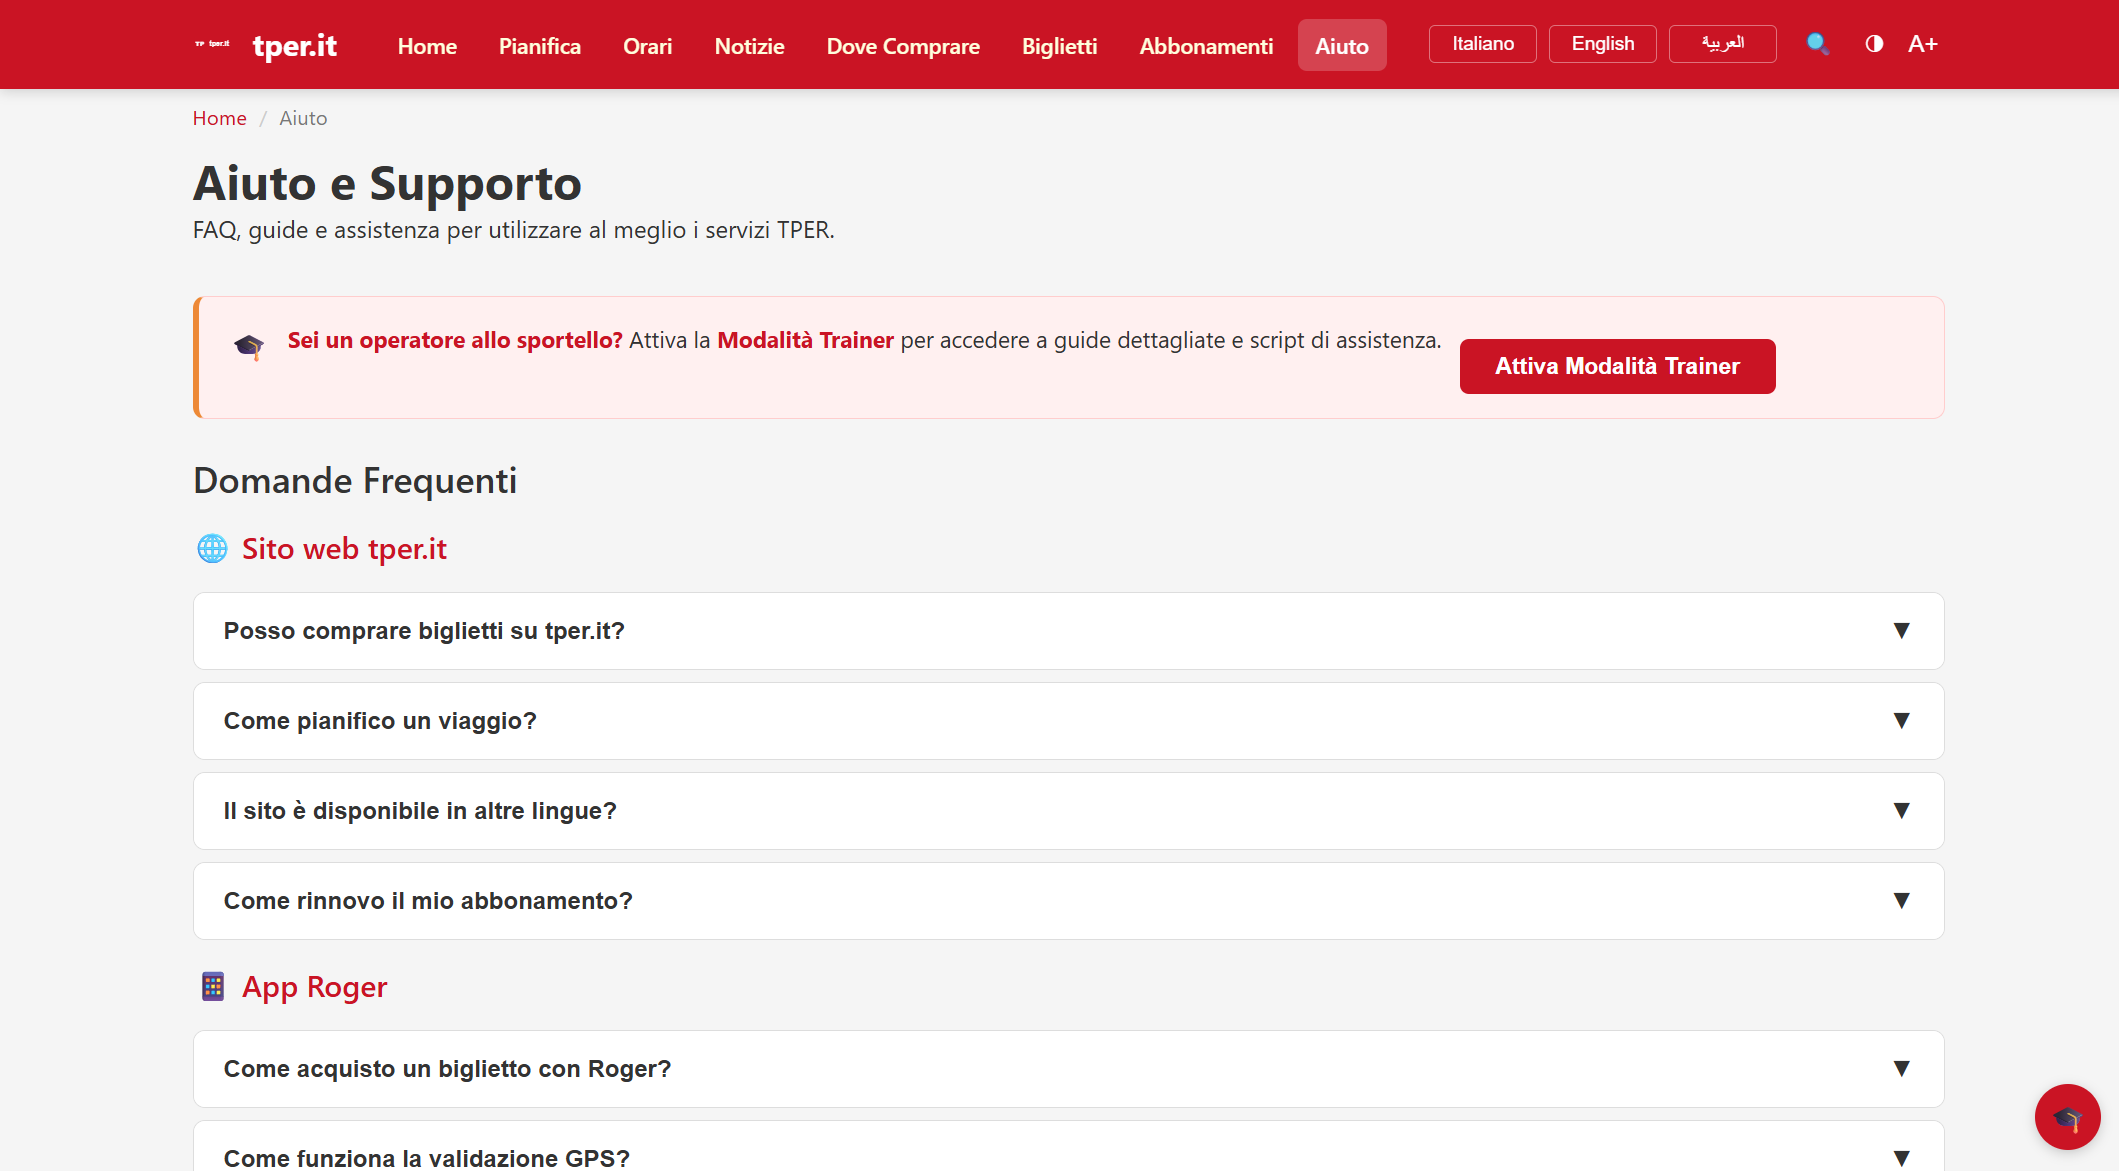
\includegraphics[width=0.85\textwidth]{Redesign Tper 2.0/Aiuto.png}
\par\small\textit{After: Help section with trainer mode, FAQ, step-by-step guides}
\caption{Trainer Mode and Support}
\label{fig:comparison-trainer}
\end{figure}

\begin{table}[H]
\centering
\small
\renewcommand{\arraystretch}{1.4}
\begin{tabular}{|p{0.5cm}|p{7cm}|p{7cm}|}
\hline
& \textbf{Before} & \textbf{After} \\ \hline
\cellcolor{primaryColor!15} &
\textit{Current support on \texttt{tper.it}} &
\textit{Trainer mode and support in tper 2.0} \\ \hline

\raisebox{0.5cm}{\rotatebox{90}{\textbf{Trainer}}} &
\textbf{Non-existent.} No assisted mode for counter operators. No step-by-step guidance mechanism to accompany users with low digital competence in navigating between channels. The only support channel is customer service (phone or email) (R4, R5). &
\textbf{Integrated sidebar} on all 22 pages of the site. 5 trainer modules: Renew, Purchase, Trip, Ticket, Top-up. Each module automatically loads the correct page with highlights on relevant elements. Activation: on request ($\mathcal{T}$ button) (R4, R5). \\ \hline

\raisebox{0.5cm}{\rotatebox{90}{\textbf{Script}}} &
No operational script for counter staff. &
5-step script for operators: (1) Identify the need, (2) Recommend the travel pass, (3) Direct to the correct channel, (4) Explain validation, (5) Confirm and ask if they need anything else (R4). \\ \hline

\raisebox{0.5cm}{\rotatebox{90}{\textbf{FAQ}}} &
Only help desk as a support channel. No interactive guidance, no organised FAQ (R10). &
\textbf{Accordion FAQ grouped by channel}: \texttt{tper.it}, Roger App, Punti Tper and Retailers, Fines, Contactless Onboard. Each section answers the most common questions for that channel. Includes direct links (e.g. from solweb FAQ $\rightarrow$ purchase page) (R9, R10). \\ \hline

\raisebox{0.5cm}{\rotatebox{90}{\textbf{Guides}}} &
Absent. &
3 step-by-step guide cards in the Help section: ``How to purchase on solweb'', ``How to use the Roger App'', ``How to find a Punto Tper''. Each with a direct CTA to the corresponding channel. Interactive wizards on Where to Buy, Tickets, and Subscriptions (R9). \\ \hline

\raisebox{0.5cm}{\rotatebox{90}{\textbf{Persistence}}} &
No session memory. If the user closes the browser or the timeout expires, they lose everything and must start over from scratch. &
\textbf{Auto-save} of the trainer session state in localStorage. The user can resume from the exact point where they left off. Printable summary with annotated screenshots and navigation path (R5, R6). \\ \hline
\end{tabular}
\caption{Trainer Mode and Support}
\label{tab:comparison-trainer}
\end{table}

\vspace{0.3cm}

% ============================================================
% COMPARISON 7: ACCESSIBILITY AND MULTILINGUAL
% ============================================================
\section{Accessibility and Multilingual Support}
\label{sec:comparison-a11y}

\textbf{R3+D3 $\rightarrow$ R8+R12} --- IT only, 10pt, <44px targets $\rightarrow$ IT/EN/AR, 14pt, WCAG AA. Chris 3/5 failed due to language.

\begin{table}[H]
\centering
\small
\renewcommand{\arraystretch}{1.4}
\begin{tabular}{|p{0.5cm}|p{7cm}|p{7cm}|}
\hline
& \textbf{Before} & \textbf{After} \\ \hline
\cellcolor{primaryColor!15} &
\textit{Current state of the \texttt{tper.it} live site} &
\textit{Accessibility and languages in tper 2.0} \\ \hline

\raisebox{0.5cm}{\rotatebox{90}{\textbf{Language}}} &
\textbf{Italian only.} No language selector, no content in English or Arabic. Foreign users completely excluded from online information services. Chris H. (English): 3/5 tasks failed despite high digital competence (R12). &
\textbf{IT + EN + AR.} Three-button language switcher always visible in the header of every page. Complete translation of labels, informational content, FAQ, and wizards. 1,600+ i18n keys in JavaScript files. RTL support for Arabic (R12). \\ \hline

\raisebox{0.5cm}{\rotatebox{90}{\textbf{Font Size}}} &
Small text (10--11pt). Reading difficulty for users over 65, particularly critical for channel names and tariffs. Maria B. could not distinguish buttons from static text (R8). &
\textbf{Minimum 14pt} on all text. \textbf{A+} button in header to further enlarge text with one click. Persistent toggle across pages (R8). \\ \hline

\raisebox{0.5cm}{\rotatebox{90}{\textbf{Contrast}}} &
Contrast not declared, likely below WCAG AA standard for some colour combinations. &
\textbf{Minimum 4.5:1 ratio} (WCAG AA). \textbf{$\blacksquare$} button to toggle high-contrast mode on all pages. Persistent toggle. Completely revised palette in high-contrast mode (R8). \\ \hline


\raisebox{0.5cm}{\rotatebox{90}{\textbf{Touch Targets}}} &
Touch targets below 44$\times$44px in many areas, making smartphone use difficult for users with reduced dexterity. &
\textbf{All interactive targets $\ge$ 44$\times$44px} (WCAG 2.1). Buttons, links, checkboxes, and radio buttons sized for error-free tactile interaction (R8). \\ \hline
\end{tabular}
\caption{Accessibility and Multilingual Support}
\label{tab:comparison-a11y}
\end{table}

\vspace{0.3cm}

% ============================================================
% COMPARISON 8: TONE AND TERMINOLOGY
% ============================================================
\section{Tone and Terminology}
\label{sec:comparison-tone}

\textbf{D3 $\rightarrow$ R9} --- Corporate terminology $\rightarrow$ User language + glosses. ``MiMuovo'', ``Sales Network'' incomprehensible to all.

\begin{table}[H]
\centering
\small
\renewcommand{\arraystretch}{1.4}
\begin{tabular}{|p{0.5cm}|p{7cm}|p{7cm}|}
\hline
& \textbf{Before} & \textbf{After} \\ \hline
\cellcolor{primaryColor!15} &
\textit{Current language on \texttt{tper.it}} &
\textit{Tone and terminology in tper 2.0} \\ \hline

\raisebox{0.5cm}{\rotatebox{90}{\textbf{Tone}}} &
Bureaucratic and institutional. Impersonal phrases, public administration lexicon. Cold and generic error messages. The user feels like an ``applicant'' rather than a customer (Issue D3). &
Encouraging and inclusive. First-person plural language: ``We'll help you choose'', ``No problem, we can try again together''. Error messages with a human tone and way out: ``Didn't find what you were looking for? Try one of these alternatives'' (R9). \\ \hline

\raisebox{0.5cm}{\rotatebox{90}{\textbf{Terms}}} &
Exclusively corporate terminology: \textit{Sales Network}, \textit{Automatic Issuing Machines}, \textit{MiMuovo}, \textit{SaltaSu}, \textit{Prontobus}, \textit{Discobus}. \texttt{solweb} and \textit{Roger} never explained or introduced. The user must know TPER jargon before using the site (Issue D3). &
\textbf{User-centric terminology with glosses}: ``Where to Buy'' (not ``Sales Network''), ``Online Subscriptions (solweb)'', ``Digital Tickets (Roger)'', ``Tobacconists and PuntoLis''. Every technical term is accompanied by an inline explanation or a tooltip on first use. The corporate name remains in parentheses for reference (R2, R9). \\ \hline

\raisebox{0.5cm}{\rotatebox{90}{\textbf{Messages}}} &
Impersonal system messages with no guidance. ``Error --- try again'' without explanation of cause or solution. The user abandons the flow (Issue D4). &
\textbf{Exponential messages} (R10): what happened, why it happened, how to fix it, what to do as an alternative. Contrast-background box with warning icon, positioned inline above the affected field. Micro-reinforcements after each step: ``Perfect, that's done!'' (R9). \\ \hline

\raisebox{0.5cm}{\rotatebox{90}{\textbf{Onboarding}}} &
No first-access path. The user lands on the homepage and must figure everything out alone. Maria B.: \textit{``I don't even know where to start''}. &
\textbf{``First Time'' Tour}: 4 illustrated screens explaining channels through everyday metaphors. Activatable from the Help button. Reassuring language: ``Don't worry, I'll show you where to go'' (R9). \\ \hline
\end{tabular}
\caption{Tone and Terminology}
\label{tab:comparison-tone}
\end{table}






% ================================================================
% Design Card: Final Reflections
% ================================================================

\newpage

\section{Design Card --- Final Reflections}
\label{sec:design-card}


\begin{tcolorbox}[colback=primaryColor,colframe=primaryColor,arc=3mm,halign=center,valign=center,height=2.5cm]
    \color{white}\LARGE\bfseries FINAL REFLECTIONS \\[0.2cm]
    \color{white!80}\large UX Design Project: Help People Help People --- TPER S.p.A. \\[0.1cm]
    \color{white!60}\normalsize Phase C --- Design Proposal
\end{tcolorbox}

\vspace{0.5cm}

\section{How Personas Influenced the Design}

The four personas developed in the Cast Card guided every design decision of Phase C. A cross-cutting theme that emerged from testing is \textbf{confusion about purchase channels}: the TPER ecosystem is structured across multiple channels (solweb, Roger, Punti Tper, tabaccherie, onboard contactless), but the informational website \texttt{tper.it} provided no guidance for orientation. Below is the specific impact of each persona on the proposed design.

\subsection{Impact of Maria Borriello (79, minimal digital literacy, SUS 27.5)}

Maria represents the project's edge case. Her 0 out of 5 completed tasks and an average time of 652 seconds per task imposed non-negotiable design constraints. Maria's main difficulty was not the purchase itself, but understanding \textbf{where} to go to make a purchase:

\begin{itemize}
    \item \textbf{Channel cards with visual icons}: Maria could not distinguish between ``solweb'', ``Roger'', and ``Punto Tper'' because these are technical names with no intuitive meaning. The redesign introduces visual cards with large icons and distinctive colors: a card with a phone symbol for Roger, a card with a computer symbol for solweb, a card with a shop symbol for Punti Tper. Each card shows only the 2--3 main operations in very simple language (``Buy ticket'', ``Top up'', ``Subscription'').
    \item \textbf{``First Visit'' guided tour}: On her first visit, Maria sees an optional introductory window: ``We'll help you get oriented'' with 4 illustrated screens that explain the channels using everyday metaphors (``Like a digital tabaccheria'', ``Like a physical shop'').
    \item \textbf{Large text and high contrast (R8)}: The reading difficulty reported in testing mandated a minimum 14pt font and 4.5:1 contrast ratio, particularly critical for reading channel names.
    \item \textbf{Encouraging tone (R9)}: Maria would abandon the task when she encountered an unfamiliar channel. The new messages guide her: ``Don't worry, let me explain where to go''.
    \item \textbf{Progress bar (R3)}: In the ``Where to Buy'' wizard, Maria always sees where she is in the selection path (``Step 2 of 3: choose how to pay'').
\end{itemize}

\subsection{Impact of Laura Palumbo (70, medium literacy, 7 errors)}

Laura demonstrated that even a few years of age difference and minimal smartphone use produce a significant performance gap. Laura possessed basic digital skills but was overwhelmed by the multitude of options:

\begin{itemize}
    \item \textbf{``Where do you want to buy?'' wizard}: Laura saw 5+ channels and did not know which to choose. The wizard reduces the choice to a guided path of 2--3 simple questions: ``What do you need?'' $\rightarrow$ ``How do you want to pay?'' $\rightarrow$ ``Here is the right channel for you''. Each answer narrows the visible options until only the recommended channel is shown.
    \item \textbf{Channel comparison table}: Laura made manual comparisons by opening 5 tabs. The ``Channel comparison'' table shows at a glance: which operations each channel supports, costs, hours, language. Filterable by desired operation (R2).
    \item \textbf{Separation of informational/transactional content}: Laura got lost between corporate news and actionable content. The homepage was reorganized by usage priority (R1), with the ``Where to Buy'' section always visible and news in a secondary section.
    \item \textbf{Clear labels (R2)}: Laura did not understand ``solweb'' and ``MyAtac'' as channel names. The redesign uses descriptive labels: ``Online Subscriptions (solweb)'', ``Digital Tickets (Roger)'' with the technical name in parentheses as support.
\end{itemize}

\subsection{Impact of Chris Harper (34, high literacy, 226 seconds on Task 1)}

Chris demonstrated that critical issues do not only affect vulnerable users. Despite high digital literacy, Chris wasted valuable time due to channel fragmentation:

\begin{itemize}
    \item \textbf{Upfront channel comparison}: Chris took 226 seconds to navigate between the various channels, visiting 3 different domains before finding the right one. The redesign shows a channel comparison table already on the homepage, allowing Chris to choose the correct channel on the first try, without exploratory navigation.
    \item \textbf{Signaled domain transition (UR-01)}: Chris would go from \texttt{tper.it} to \texttt{solweb.tper.it} without warning and had to reorient. The redesign shows an explicit notice before every redirect: ``You are about to go to \texttt{solweb.tper.it} to complete the subscription purchase'' with a ``Continue'' button and a ``Go back'' button.
    \item \textbf{``Did you mean...?'' cross-links}: Chris often ended up on the wrong channel because the names were ambiguous. The system now recognizes intent: if the user searches for ``subscription'' on a \texttt{tper.it} informational page, a direct link appears: ``Are you trying to buy a subscription? Go to \texttt{solweb.tper.it}'' (UR-03).
    \item \textbf{Preventive checklist (R11)}: Chris had to independently search for which documents were needed for the subscription. The redesign shows a visual ``Required documents'' checklist already in the informational guide, before redirecting to solweb.
\end{itemize}

\subsection{Impact of Fatima Hassan (45, Arabic speaker)}

Fatima highlighted language barriers in navigating between channels, not just in using services:

\begin{itemize}
    \item \textbf{Multilingual channel guide (R12)}: The ``Where to Buy'' guide is fully translated into Arabic and English, including channel descriptions, operation names, and wizard messages. Fatima can choose the right channel in her own language without having to interpret Italian terms.
    \item \textbf{Multi-language synonym search}: The search engine accepts ``biglietto'', ``ticket'', and ``tadhkira'' (ticket in Arabic) and returns the same results, with an indication of the appropriate channel for each purchase type.
    \item \textbf{Universal visual signage}: Channel icons have been designed to be culturally neutral and universally recognizable: phone for Roger, building for Punto Tper, computer for solweb, credit card for contactless. They reduce dependence on written language.
    \item \textbf{Multilingual QR code}: The QR code on a Punto Tper receipt lands on an informational page that detects the device language and automatically presents itself in Arabic, English, or Italian.
\end{itemize}

\vspace{0.3cm}

\section{How Use Cases Influenced the Design}

The Use Cases (UR-01--UR-05) emerging from the Cast Card guided the design choices, with particular attention to channel fragmentation and the resulting confusion:

\begin{itemize}
    \item \textbf{UR-01 (Channel fragmentation)}: Led to the design of \texttt{tper.it} as an \textbf{integrated information hub}. Instead of isolating each channel, the redesign presents a unified view of the TPER ecosystem, with a card for each channel, the supported operations, and direct links. The explicit transition notice prepares the user for the context change.
    \item \textbf{UR-02 (Post-purchase confusion)}: Generated the ``After Purchase'' section for each channel. On \texttt{tper.it}, every product page includes a post-purchase guide: ``Just bought on solweb? Here is how to activate the subscription'' or ``Topped up at a tabaccheria? Check your remaining balance on Roger'' (R6).
    \item \textbf{UR-03 (Wrong-channel errors)}: Led to the implementation of \textbf{intelligent cross-links}. When a user visits an informational page on \texttt{tper.it} describing a product purchasable elsewhere, the system shows a contextual suggestion: ``Did you mean to buy? Go to [correct channel]''. This reduces navigation errors and abandonment (R10).
    \item \textbf{UR-04 (Physical/digital bridge)}: Inspired the \textbf{QR code} system that connects the physical experience (Punto Tper) to the informational one (\texttt{tper.it}). The receipt printed at the counter includes a QR code that leads to the dedicated informational page, with an operation summary, attached documents, and the possibility to continue digitally. The bridge is bidirectional: from the informational page, one can book an appointment at the nearest Punto Tper.
    \item \textbf{UR-05 (Subscription guide)}: Generated the step-by-step ``How to Subscribe'' guide in 5 phases, entirely hosted on \texttt{tper.it} as informational content. Each phase explains what is needed, which documents to prepare, and, at the end, redirects the user to the correct channel (solweb for online purchase, Punto Tper for in-person purchase). Includes an ``Are you eligible for a discount?'' calculator that assesses user eligibility in under a minute.
\end{itemize}

\vspace{0.3cm}

\section{Reflections on the Design Process}

\subsection{Consistency Across Phases}

Phase C is the culmination of a journey that began with the Ethnographic Assessment (Phase A) and continued with the Feasibility Study (Phase B). Every design decision is traceable to the collected evidence:

\begin{itemize}
    \item From user testing $\rightarrow$ to recommendations R1--R13 $\rightarrow$ to Information Architecture $\rightarrow$ to Blueprint $\rightarrow$ to Wireframes.
    \item The Issues (D1--D5, R1--R4) identified in the heuristic analysis found a response in one or more recommendations.
    \item The Personas did not stay as an academic exercise: they guided concrete choices regarding IA depth, text size, language, and navigation modes.
\end{itemize}

\subsection{Critical Decisions}

Some decisions required balancing conflicting needs:

\begin{itemize}
    \item \textbf{Channel guide vs. freedom of choice}: The ``Where to Buy'' wizard guides the user toward the optimal channel, but some expert users (like Chris) might prefer free choice. The solution is to show the recommended channel prominently, but always list all alternatives in an ``Other ways to buy'' section.
    \item \textbf{Information hub vs. corporate content}: Keeping \texttt{tper.it} as a purely informational site means that corporate news and press releases must find space without obscuring the main functions. The choice was to relegate them to a separate ``Company'' section accessible from the footer, while the entire main area is dedicated to the user.
    \item \textbf{Informational completeness vs. simplicity}: Describing 5+ channels with all their nuances risks reproducing the original problem (information overload). The compromise is the filterable comparison table: the user sees everything but can narrow the field by operation type or payment method.
    \item \textbf{Explicit redirects vs. seamless experience}: Showing a warning before redirecting to solweb adds a step, but reduces the disorientation of the domain change. The test with Chris demonstrated that the cost in terms of additional clicks is negligible compared to the benefit of knowing where one is going.
\end{itemize}

\subsection{Contribution of Personas to the Design}

The most significant contribution of the personas was making design decisions ``personal''. When having to choose between two options, the question ``What would Maria do?'' or ``What would Fatima understand?'' provided an unequivocal compass. This ensured that the design remained user-centered even in the most abstract technical choices.

In particular, the theme of \textbf{channel confusion} --- which emerged across all four personas --- became the fulcrum of \texttt{tper.it}'s informational redesign. It was not about improving the purchase (which happens elsewhere), but about acting as an \textbf{informational bridge} between the user and the right channel. This redefined the very mission of the site: no longer a generic information container, but an \textbf{active guide to the TPER ecosystem}.

\subsection{Limitations and Future Developments}

\begin{itemize}
    \item The presented wireframes are in lo-fi format. High-fidelity prototyping with summative user testing is the natural next step (Phase D).
    \item The channel guide and the ``Where to Buy'' wizard are designed to be tested with real users (Maria, Laura, Chris, Fatima) to validate their effectiveness in reducing channel confusion.
    \item The QR code bridge between Punto Tper and \texttt{tper.it} requires technical integration with the physical counter's management system. Technical feasibility was verified in Phase B, but remains to be implemented.
    \item The ``Did you mean...?'' cross-links require an intent recognition engine based on user navigation. A first version can be implemented with static rules, but the natural evolution is the use of machine learning for predictive suggestions.
\end{itemize}

\vspace{0.5cm}

\begin{center}
{\color{secondaryColor}\small
Document describing the impact of personas and use cases on the proposed design \\[4pt]
\textbf{Phase C --- Design Proposal: Final Reflections} \\[4pt]
Project: UX Design Project: Help People Help People --- TPER S.p.A.}
\end{center}


% ================================================================
% Design Summary Card
% ================================================================

\newpage
\section{Design Summary Card}
\label{sec:design-summary}

\begin{tcolorbox}[colback=primaryColor,colframe=primaryColor,arc=1.5mm,halign=center,valign=center,height=2cm]
 \color{white}\LARGE\bfseries\sffamily DESIGN SUMMARY \\[0.1cm]
 \color{white!80}\small\sffamily Phase C --- Design Proposal
\end{tcolorbox}

\vspace{0.3cm}

\subsection*{Design Versions as Submitted}

\begin{table}[H]
\centering
\small
\renewcommand{\arraystretch}{1.3}
\begin{tabular}{|p{2.2cm}|p{3.2cm}|p{2.8cm}|p{4.2cm}|}
\hline
\textbf{Version} & \textbf{Folder} & \textbf{Date / Time} & \textbf{Evaluation Types} \\
\hline
\textbf{V0} 
& \texttt{Website - Finale/} (initial state)
& June 12, 2026, 18:00
& Before formal evaluation \\
\hline
\textbf{V1} 
& \texttt{Website - Finale/} (post-FT fix)
& June 22, 2026, 12:00
& Inspection evaluation --- Cognitive Walkthrough (CW-01--CW-11) \\
\hline
\textbf{Final (v2.0)} 
& \texttt{Website - Finale/} (final version)
& July 3, 2026, 10:00
& \parbox{3.8cm}{\raggedright --- Cognitive Walkthrough (Post-Fix) \\ --- Formative Test (2 subjects) \\ --- Summative Test (2 subjects)} \\
\hline
\end{tabular}
\caption{Design versions submitted for evaluation}
\label{tab:design-versions}
\end{table}

\vspace{0.3cm}

\subsection*{List of Issues Handled During Redesign, Ordered by Importance}

\renewcommand{\arraystretch}{1.3}
\begin{longtable}{|p{0.8cm}|p{3cm}|p{3.5cm}|p{6.5cm}|}
\hline
\textbf{\#} & \textbf{Issue} & \textbf{Ref. Requirement / Test} & \textbf{Wireframe / Blueprint affected} \\
\hline
\endhead
1 & Terminology ambiguity ``Where to Buy'' vs ``Subscriptions'' (\textbf{FT1}, P=5, I=5) 
& Phase A: R1 (Task-Oriented Home Page) \\
& Phase B: Cast Card --- UR-03 \\
 & WF1 (Homepage --- ``What do you want to do?'' grid and channel sidebar) \\
& BP1 (Information Architecture: purchase vs informational sections) \\
& BP3 (User Journey: decision point ``where to buy?'') \\
\hline
2 & Confusion between purchase channels: user does not know which channel to use (\textbf{D2}, R4) 
& Phase A: R2 (Flat IA), R4 (Trainer-Mode) \\
& Phase B: Cast Card --- UR-01 \\
 & Phase D: FT2
 & WF3 (Where to Buy --- channel cards with icons) \\
& BP2 (Multi-Channel Ecosystem: relationships and bridges) \\
\hline
3 & No step-by-step guide for complex operations (\textbf{R5}) 
& Phase A: R5 (Progress Persistence) \\
& Phase B: Cast Card --- UR-05 \\
 & WF5 (Help + Trainer-Mode: 5-step guide) \\
& BP3 (Trainer-Mode intervention along the journey) \\
\hline
4 & Overloaded homepage: company news obscures primary functions (\textbf{D1}, R1) 
& Phase A: R1 (Task-Oriented Home Page) \\
 & WF1 (Homepage: hero search + 4 service cards, news in footer) \\
& BP1 (IA: section reorganization by usage priority) \\
\hline
5 & Terminology barrier: ``solweb'', ``Roger'' as technical names (\textbf{D3}, R2) 
& Phase A: R2 (Descriptive Labels) \\
& Phase B: Cast Card --- Laura, Maria \\
& Phase D: FT1
& WF3 (Channel cards: ``Online subscriptions (solweb)'') \\
& BP2 (Ecosystem: user-centric labeling) \\
\hline
6 & Lack of feedback and error recovery (\textbf{D4}, R10) 
& Phase A: R10 (Exponential Error Messages) \\
 & BP3 (Decision points with recovery messages) \\
& WF5 (Trainer-Mode: encouraging messages) \\
\hline
7 & Mandatory authentication for basic operations (\textbf{D5}, R7) 
& Phase A: R7 (Guest Path) \\
 & BP1 (IA: sections accessible without login) \\
& WF1 (Channel sidebar always visible, even in guest mode) \\
\hline
8 & No multilingual support for foreign users (\textbf{R12}) 
& Phase A: R12 (English and Arabic) \\
& Phase B: Cast Card --- Fatima Hassan
& WF3 (Channel cards and wizard translated into EN/AR) \\
& BP2 (Ecosystem: bridge with multilingual content) \\
\hline
9 & Required documentation not communicated to the user in advance (\textbf{R11}) 
& Phase A: R11 (Preventive Checklist) \\
 & WF4 (Tickets: ``Required documents'' badge) \\
& BP3 (Checklist before redirect to solweb) \\
\hline
10 & No ``First Access'' onboarding (\textbf{FT2}, P=2, I=3) 
& Phase D: FT2, FT6
& WF5 (Guided Tour ``First Time'' 4 screens) \\
& BP3 (Entry point: onboarding before navigation) \\
\hline
\end{longtable}

\vspace{0.3cm}

\begin{tcolorbox}[colback=primaryColor!5,colframe=primaryColor,arc=2mm]
\small
\textbf{Note:} Each issue is related to the requirements from Phase A (R1--R13), Phase B (Cast Card --- Use Case UR-01--UR-05) and Phase D (Cognitive Walkthrough CW-01--CW-11, Formative Test FT1--FT7). The design solutions can be located in the wireframes (WF1--WF7b) and blueprints (BP1--BP3).
\end{tcolorbox}

% ================================================================
% Phase D2: Inspection Card (Cognitive Walkthrough)
% ================================================================

\newpage

\section{Cognitive Walkthrough --- Inspection Card}
\label{sec:inspection-card}


\newcolumntype{L}[1]{>{\raggedright\arraybackslash}p{#1}}
\newcolumntype{C}[1]{>{\centering\arraybackslash}p{#1}}

\begin{tcolorbox}[colback=primaryColor,colframe=primaryColor,arc=3mm,halign=center,valign=center,height=2.5cm]
 \color{white}\LARGE\bfseries INSPECTION CARD \\[0.2cm]
 \color{white!80}\large UX Design Project: Help People Help People --- TPER S.p.A. \\[0.1cm]
 \color{white!60}\normalsize Phase D --- Cognitive Walkthrough
\end{tcolorbox}

\vspace{0.3cm}

% =====================================================================
% INSPECTION DATA (aligned to template)
% =====================================================================
\section{Inspection Data}

\begin{tcolorbox}[colback=backgroundColor,colframe=borderColor,arc=2mm]
\small

\noindent\textbf{Name of version:} TPER Redesign --- v1.0 (Phase C -- Design Proposal)

\vspace{0.3cm}
\noindent\textbf{Inspection context data:}
\begin{itemize}
 \item \textbf{Date:} June 15--16, 2026
 \item \textbf{Team members:} 2 evaluators (design team members)
 \item \textbf{Roles:} Evaluator 1 (narrator, guides the simulation), Evaluator 2 (listener, records critical issues)
 \item \textbf{Mode:} Individual evaluation on static prototype (HTML/CSS), followed by comparison and consensus
\end{itemize}

\vspace{0.3cm}
\noindent\textbf{Inspection method:}
\begin{itemize}
 \item[$\bullet$] \textbf{Cognitive Walkthrough} (selected)
 \item[$\circ$] Formal Action Analysis
 \item[$\circ$] Informal Action Analysis
 \item[$\circ$] Heuristic Analysis
\end{itemize}

\vspace{0.3cm}
\noindent\textbf{Output of inspection:} The 5 analyzed tasks are documented below. For each step, the 4 CW questions (Goal, Visibility, Mapping, Feedback) are evaluated. A qualitative justification is provided for each critical issue detected.

\end{tcolorbox}

\vspace{0.3cm}

% =====================================================================
% INTRODUCTION TO COGNITIVE WALKTHROUGH
% =====================================================================
\section{Introduction to the Cognitive Walkthrough}

\begin{tcolorbox}[colback=backgroundColor,colframe=borderColor,arc=2mm]
\small
The Cognitive Walkthrough is an inspection method that evaluates learnability through simulated task execution. For each step, 4 questions are answered (Goal, Visibility, Mapping, Feedback). Evaluators simulate the profiles of the personas defined in Phase B, assuming minimal digital literacy and a domestic context without assistance.

\vspace{0.2cm}
\noindent\textbf{Selected tasks:}
\begin{enumerate}
 \item Subscription Renewal (Guest Flow)
 \item Subscription Purchase (Login Flow)
 \item Discovering Concessions
 \item Purchase Guide (Where to Buy)
 \item Card Verification and Top-up
\end{enumerate}
\end{tcolorbox}

\vspace{0.5cm}

% =====================================================================
% TASK 1: SUBSCRIPTION RENEWAL (GUEST)
% =====================================================================
\section{Task 1: Subscription Renewal --- Guest Flow}

\begin{tcolorbox}[colback=primaryColor!10,colframe=primaryColor,arc=2mm]
\small
\textbf{User profile:} Liliana (70, low digital literacy) needs to renew her monthly subscription that expires tomorrow. She tries to do it on her own, without assistance.

\textbf{Starting point:} Homepage \texttt{tper.it}. \textbf{Goal:} Complete the renewal without registration.
\end{tcolorbox}

\vspace{0.3cm}

\subsection{Step 1: Finding the ``Where to Buy'' section}

\begin{tcolorbox}[colback=backgroundColor,colframe=borderColor,arc=2mm]
\small
\begin{tabular}{|L{3cm}|L{11cm}|}
\hline
\textbf{User action} & \multicolumn{1}{L{11cm}|}{From the homepage, clicks ``Where to Buy'' in the main navigation or on the ``Where to Buy'' card in the ``What do you want to do?'' grid} \\
\hline
\textbf{Q1 -- Goal} & The user wants to renew a subscription. The term ``Where to Buy'' may not be immediately associated with renewal. \\
\hline
\textbf{Q2 -- Visibility} & The ``Where to Buy'' item is clearly visible in the main menu (position \#4) and as a card on the homepage (green card with cart icon). \\
\hline
\textbf{Q3 -- Mapping} & ``Where to Buy'' suggests purchase, not renewal. The user may hesitate. However, the ``Subscriptions'' card (purple card) is closer to the concept of ``subscription renewal''. \\
\hline
\textbf{Q4 -- Feedback} & Navigation is a simple page transition, no specific feedback. \\
\hline
\end{tabular}

\vspace{0.3cm}
\noindent\textbf{Critical issue:} Q3 is critical: the term ``Where to Buy'' is ambiguous for a renewal operation. The user might click ``Subscriptions'' instead of ``Where to Buy'', moving away from the guided channel selection flow. Although ``Subscriptions'' provides fare information, it does not lead directly to the renewal channel, requiring an additional navigation step.
\end{tcolorbox}

\vspace{0.3cm}

\subsection{Steps 2--3: Using the interactive guide}

\begin{tcolorbox}[colback=backgroundColor,colframe=borderColor,arc=2mm]
\small
\noindent The user clicks ``We'll help you choose'' and answers the 3 questions (service, channel, payment). No critical issues: the guide is clear, options are large and clickable, the ``Question X of 3'' progress bar and the ``Back'' button provide adequate feedback. The wizard takes the user to the result ``solweb.tper.it'' with a direct link.
\end{tcolorbox}

\vspace{0.3cm}

\subsection{Step 4: Reaching solweb and choosing ``Impersonal Renewal''}

\begin{tcolorbox}[colback=backgroundColor,colframe=borderColor,arc=2mm]
\small
\begin{tabular}{|L{3cm}|L{11cm}|}
\hline
\textbf{User action} & \multicolumn{1}{L{11cm}|}{From the guide, gets ``solweb.tper.it'' as the result. Clicks ``Go to solweb'' which leads to \texttt{login.html}. Here, clicks ``Impersonal Renewal'' among the 4 Quick Actions, arriving at \texttt{rinnova.html}. Chooses ``Impersonal Subscription'' and then ``Renew without Login''.} \\
\hline
\textbf{Q1 -- Goal} & The user wants to renew without creating an account. ``Impersonal Renewal'' and ``Renew without Login'' match this need. \\
\hline
\textbf{Q2 -- Visibility} & The ``Quick Actions'' are in a clearly visible section under the login form, with large buttons. The decision screen on \texttt{rinnova.html} shows two side-by-side cards with clear icons and descriptions. \\
\hline
\textbf{Q3 -- Mapping} & ``Impersonal Subscription'' $\rightarrow$ ``Non-nominative. You just need your card number'' $\rightarrow$ ``Renew without Login''. The language is simple and descriptive. \\
\hline
\textbf{Q4 -- Feedback} & The progress bar shows ``Step 1 of 2''. The breadcrumb shows ``Login / Impersonal Renewal''. Good orientation. \\
\hline
\end{tabular}

\vspace{0.3cm}
\noindent The guest flow is clear, options are well explained. The user has a direct path for renewal without needing to create an account.

\vspace{0.2cm}
\noindent\textbf{Critical issue:} \textbf{CW-08 (Medium, Q2).} On \texttt{login.html}, the Quick Actions are at the bottom of the page, below the login form that visually dominates the screen. For Liliana, the login form is the focal point: she risks not noticing the guest options, attempting to log in without credentials, and abandoning the task.
\end{tcolorbox}

\vspace{0.3cm}

\subsection{Step 5: Filling in the renewal form}

\begin{tcolorbox}[colback=backgroundColor,colframe=borderColor,arc=2mm]
\small
\begin{tabular}{|L{3cm}|L{11cm}|}
\hline
\textbf{User action} & \multicolumn{1}{L{11cm}|}{Enters the card number (format TPER-XXXXXX) and clicks ``Confirm and Proceed''} \\
\hline
\textbf{Q1 -- Goal} & The user understands they must enter the card number to identify the subscription to be renewed. \\
\hline
\textbf{Q2 -- Visibility} & The ``Card Number / Subscription Code'' field is the only field on the form. Clearly visible with label and placeholder. \\
\hline
\textbf{Q3 -- Mapping} & ``Card number'' $\rightarrow$ ``identify my subscription'' is a clear mapping. Many users are familiar with this type of form (e.g., phone top-ups). \\
\hline
\textbf{Q4 -- Feedback} & Validation is client-side: if the field is empty, it shows an inline error (\texttt{showFieldError}). On submit, redirect to \texttt{pagamento.html}. Quick feedback. \\
\hline
\end{tabular}

\vspace{0.3cm}
\noindent Minimal and clear form.

\vspace{0.2cm}
\noindent\textbf{Issue identified:} The format ``TPER-XXXXXX'' has no formal client-side validation. A user who enters an incorrect format (e.g., numbers only) will still be redirected to payment, only to discover the error later. It is recommended to add a validation regex with immediate feedback.
\end{tcolorbox}

\vspace{0.3cm}


\vspace{0.3cm}

% =====================================================================
% TASK 2: SUBSCRIPTION PURCHASE (LOGIN FLOW)
% =====================================================================
\section{Task 2: Subscription Purchase --- Login Flow}

\begin{tcolorbox}[colback=primaryColor!10,colframe=primaryColor,arc=2mm]
\small
\textbf{User profile:} David (34, English speaker, high digital literacy) wants to buy an annual subscription. He already has a solweb account. He tries to do everything on his own.

\textbf{Starting point:} ``Where to Buy'' page on \texttt{tper.it}. \textbf{Goal:} Complete the purchase through to confirmation.
\end{tcolorbox}

\vspace{0.3cm}

\subsection{Step 1: Reaching login and signing in}

\begin{tcolorbox}[colback=backgroundColor,colframe=borderColor,arc=2mm]
\small
\begin{tabular}{|L{3cm}|L{11cm}|}
\hline
\textbf{User action} & \multicolumn{1}{L{11cm}|}{From ``Where to Buy'', clicks ``Go to solweb.tper.it'' $\rightarrow$ \texttt{login.html}. Enters email/CF and password, then clicks ``Sign in''.} \\
\hline
\textbf{Q1 -- Goal} & The user knows they must sign in to buy a subscription. The informational banner ``To purchase a subscription, you must sign in'' confirms this. \\
\hline
\textbf{Q2 -- Visibility} & The login form is the main content of the page. The ``Fiscal Code / Email'' and ``Password'' fields are clearly visible. \\
\hline
\textbf{Q3 -- Mapping} & ``Enter your credentials'' $\rightarrow$ ``sign in to your account'' is the universal login mapping. The user recognizes it. However, for an English-speaking user, ``Fiscal Code'' is an unfamiliar Italian concept. \\
\hline
\textbf{Q4 -- Feedback} & On submit, immediate redirect to \texttt{dashboard.html?login=ok}. Clear feedback of successful login. In case of error, an error message with explanation and alternatives. \\
\hline
\end{tabular}

\vspace{0.3cm}
\noindent\textbf{Critical issue:} Q3 is critical: ``Fiscal Code'' is not an international concept. The English-speaking user may not understand what to enter. The placeholder ``or Email'' only partially mitigates the problem: the user must still pause, read, and interpret before finding the alternative.
\end{tcolorbox}

\vspace{0.3cm}

\subsection{Step 2: Dashboard and plan selection}

\begin{tcolorbox}[colback=backgroundColor,colframe=borderColor,arc=2mm]
\small
\begin{tabular}{|L{3cm}|L{11cm}|}
\hline
\textbf{User action} & \multicolumn{1}{L{11cm}|}{On the dashboard (2 cards: ``Purchase'', ``Personal Renewal''), clicks ``Purchase'' $\rightarrow$ \texttt{piani.html} with 3 plans: Monthly (51\euro), Annual (390\euro), Suburban (from 35\euro/month). Chooses Annual and clicks ``Buy Online''.} \\
\hline
\textbf{Q1 -- Goal} & The user wants to buy. ``Purchase'' on the dashboard is explicit. The plans show clear prices and descriptions. \\
\hline
\textbf{Q2 -- Visibility} & The plan cards are large, with highlighted prices and ``Select'' buttons. The progress bar shows ``Step 2 of 4''. \\
\hline
\textbf{Q3 -- Mapping} & ``Select'' on the annual plan $\rightarrow$ ``I want this subscription'' is direct and unambiguous. \\
\hline
\textbf{Q4 -- Feedback} & The progress bar updates, the breadcrumb shows the path. On click, redirect to \texttt{documenti.html}. \\
\hline
\end{tabular}

\vspace{0.3cm}
\noindent Linear flow, visible prices, clear selection.
\end{tcolorbox}

\vspace{0.3cm}

\subsection{Step 3: Document upload}

\begin{tcolorbox}[colback=backgroundColor,colframe=borderColor,arc=2mm]
\small
\begin{tabular}{|L{3cm}|L{11cm}|}
\hline
\textbf{User action} & \multicolumn{1}{L{11cm}|}{On \texttt{documenti.html}, sees the required documents checklist (ID, fiscal code, ID photo). Confirms they have them and clicks ``Proceed to Payment''.} \\
\hline
\textbf{Q1 -- Goal} & The user understands that some documents are needed for the annual subscription. The checklist shows them. \\
\hline
\textbf{Q2 -- Visibility} & The checklist is well structured with icons, descriptions, and notes. \\
\hline
\textbf{Q3 -- Mapping} & ``Do I have these documents?'' $\rightarrow$ ``Confirm and proceed''. The mapping is clear: the user verifies they have what is needed. \\
\hline
\textbf{Q4 -- Feedback} & Progress bar ``Step 3 of 4''. On submit, redirect to \texttt{pagamento.html}. Feedback OK. \\
\hline
\end{tabular}

\vspace{0.3cm}
\noindent The preventive checklist is a good solution to the ``arriving at the counter without documents'' problem.
\end{tcolorbox}

\vspace{0.3cm}

\subsection{Step 4: Payment and confirmation}

\begin{tcolorbox}[colback=backgroundColor,colframe=borderColor,arc=2mm]
\small
\begin{tabular}{|L{3cm}|L{11cm}|}
\hline
\textbf{User action} & \multicolumn{1}{L{11cm}|}{On \texttt{pagamento.html}, sees the order summary (annual plan 390\euro), enters payment details (card, expiry, CVV), clicks ``Pay 390\euro'' $\rightarrow$ redirect to \texttt{conferma.html} with summary and PDF receipt.} \\
\hline
\textbf{Q1 -- Goal} & The user wants to pay to complete the purchase. The summary and total are clearly visible. \\
\hline
\textbf{Q2 -- Visibility} & Complete payment form (cardholder, card number, expiry, CVV). ``Pay'' button with clearly visible amount. \\
\hline
\textbf{Q3 -- Mapping} & ``Fill in your card details'' $\rightarrow$ ``pay the amount shown'' is the e-commerce standard. Universal mapping. \\
\hline
\textbf{Q4 -- Feedback} & After payment, redirect to \texttt{conferma.html} with order summary, confirmation message, and link to download the PDF receipt. Excellent feedback. \\
\hline
\end{tabular}

\vspace{0.3cm}
\noindent Standard and reassuring payment flow.

\vspace{0.2cm}
\noindent\textbf{Issue identified:} \textbf{CW-03 (Medium).} The ``And now? What to do after purchase'' section is present at the bottom of the confirmation page, but it is not very visible: located below the order summary and the receipt download button, it requires the user to scroll below the fold. A user with low digital literacy may not notice the post-purchase instructions and board without a properly usable ticket.
\end{tcolorbox}

\vspace{0.3cm}


\vspace{0.3cm}

% =====================================================================
% TASK 3: DISCOVERING CONCESSIONS
% =====================================================================
\section{Task 3: Discovering Concessions}

\begin{tcolorbox}[colback=primaryColor!10,colframe=primaryColor,arc=2mm]
\small
\textbf{User profile:} Roberto (45, low motivation, low concentration) has heard he might be eligible for a discount on his subscription.

\textbf{Starting point:} ``Subscriptions'' page on \texttt{tper.it}. \textbf{Goal:} Find out if he is eligible for concessions and which documents are needed.
\end{tcolorbox}

\vspace{0.3cm}

\subsection{Step 1: Noticing the concessions banner}

\begin{tcolorbox}[colback=backgroundColor,colframe=borderColor,arc=2mm]
\small
\begin{tabular}{|L{3cm}|L{11cm}|}
\hline
\textbf{User action} & \multicolumn{1}{L{11cm}|}{On the ``Subscriptions'' page, sees a green banner with a trophy icon: ``Not sure if you're eligible for a discount? Discover in 30 seconds which concessions you can access'' with a ``Discover Concessions'' button.} \\
\hline
\textbf{Q1 -- Goal} & The user wants to know if they are eligible for discounts. The banner speaks exactly about this. \\
\hline
\textbf{Q2 -- Visibility} & The banner is at the top of the page, colored (green), with an appealing icon and short text. Very visible. \\
\hline
\textbf{Q3 -- Mapping} & ``Discover Concessions'' $\rightarrow$ ``find out if I am eligible for discounts'' is a direct and clear mapping. \\
\hline
\textbf{Q4 -- Feedback} & Click $\rightarrow$ navigation to \texttt{agevolazioni.html}. Standard page transition. \\
\hline
\end{tabular}

\vspace{0.3cm}
\noindent Well-designed banner: visible, targeted, with a clear CTA.
\end{tcolorbox}

\vspace{0.3cm}

\subsection{Step 2: Launching the wizard and answering questions}

\begin{tcolorbox}[colback=backgroundColor,colframe=borderColor,arc=2mm]
\small
\begin{tabular}{|L{3cm}|L{11cm}|}
\hline
\textbf{User action} & \multicolumn{1}{L{11cm}|}{On \texttt{agevolazioni.html}, clicks ``Discover My Concessions'' $\rightarrow$ answers 4 questions (age, ISEE, residence, travel frequency) by clicking on the options.} \\
\hline
\textbf{Q1 -- Goal} & The user understands that answering simple questions will lead to a personalized result. \\
\hline
\textbf{Q2 -- Visibility} & The questions are large, one at a time, with button options. The ``Question X of 4'' progress bar is visible. \\
\hline
\textbf{Q3 -- Mapping} & ``How old are you?'' $\rightarrow$ select the age range. ``Are you a resident of Bologna?'' $\rightarrow$ simple options. Questions in natural language, not bureaucratic. \\
\hline
\textbf{Q4 -- Feedback} & On clicking each answer, the next question appears immediately. ``Back'' button available. Progress bar updated. Excellent feedback. \\
\hline
\end{tabular}

\vspace{0.3cm}
\noindent Simple wizard, clear questions, non-technical language. The user does not need to know bureaucratic terms to answer.
\end{tcolorbox}

\vspace{0.3cm}

\subsection{Step 3: Reading the results}

\begin{tcolorbox}[colback=backgroundColor,colframe=borderColor,arc=2mm]
\small
\begin{tabular}{|L{3cm}|L{11cm}|}
\hline
\textbf{User action} & \multicolumn{1}{L{11cm}|}{Sees the results screen: ``We found X concessions for you!'' with a card for each concession, description, required documents, and a ``View Subscriptions'' link.} \\
\hline
\textbf{Q1 -- Goal} & The user wants to know if they are eligible for discounts. The results tell them clearly. \\
\hline
\textbf{Q2 -- Visibility} & The results are in colored cards with title, description, and icon. The required documents are listed. \\
\hline
\textbf{Q3 -- Mapping} & ``You are eligible for...'' $\rightarrow$ ``Here is what you need''. The connection is direct: the user understands what to do next. \\
\hline
\textbf{Q4 -- Feedback} & Success message with the number of concessions found. ``Restart'' button to redo the test. ``View Subscriptions'' link for further details. \\
\hline
\end{tabular}

\vspace{0.3cm}
\noindent Personalized, clear result, with an explicit call-to-action.

\vspace{0.2cm}
\noindent\textbf{Issue identified:} \textbf{CW-05 (Minor).} The result does not include a ``Print'' button to take the document list to the counter. For elderly or low-digital-literacy users, paper support is important.

\vspace{0.2cm}
\noindent\textbf{Issue:} \textbf{CW-10 (Medium, Q4).} If the wizard finds no concessions, the message ``No automatic concessions found'' may be perceived as failure. For Roberto (low motivation), this confirms the pointlessness of the attempt. A digital alternative that keeps the user in the flow is missing.
\end{tcolorbox}

\vspace{0.3cm}


\vspace{0.3cm}

% =====================================================================
% TASK 4: PURCHASE GUIDE (WHERE TO BUY)
% =====================================================================
\section{Task 4: Purchase Guide --- Where to Buy}

\begin{tcolorbox}[colback=primaryColor!10,colframe=primaryColor,arc=2mm]
\small
\textbf{User profile:} Fatima (68, Arabic speaker, illiterate in written Italian, minimal digital literacy) visits \texttt{tper.it} for the first time. She does not know the site is informational only. She is looking for a way to ``buy a bus ticket''.

\textbf{Starting point:} Homepage \texttt{tper.it}. \textbf{Goal:} Discover how and where to buy a ticket.
\end{tcolorbox}

\vspace{0.3cm}

\subsection{Step 1: Finding the ``Where to Buy'' section}

\begin{tcolorbox}[colback=backgroundColor,colframe=borderColor,arc=2mm]
\small
\begin{tabular}{|L{3cm}|L{11cm}|}
\hline
\textbf{User action} & \multicolumn{1}{L{11cm}|}{From the homepage, clicks ``Where to Buy'' (green card or navigation).} \\
\hline
\textbf{Q1 -- Goal} & Fatima wants to ``buy''. ``Where to Buy'' exactly matches her need. For a user with 1/5 literacy, the ``Where to Buy'' language is perfect. \\
\hline
\textbf{Q2 -- Visibility} & The ``Where to Buy'' card is the second in the ``What do you want to do?'' grid, clearly visible right after the hero section. Cart icon + clear title. \\
\hline
\textbf{Q3 -- Mapping} & ``Where to Buy'' $\rightarrow$ ``find out where to buy'' is literal and unambiguous. \\
\hline
\textbf{Q4 -- Feedback} & Navigation to \texttt{dove-comprare.html}. The page opens with the explanation that \texttt{tper.it} does not sell directly. \\
\hline
\end{tabular}

\vspace{0.3cm}
\noindent``Where to Buy'' is the best labeling choice for users with low literacy.
\end{tcolorbox}

\vspace{0.3cm}

\subsection{Step 2: Reading the informational banner}

\begin{tcolorbox}[colback=backgroundColor,colframe=borderColor,arc=2mm]
\small
\begin{tabular}{|L{3cm}|L{11cm}|}
\hline
\textbf{User action} & \multicolumn{1}{L{11cm}|}{Arriving on the page, reads the text: ``On tper.it it is not possible to purchase travel passes. This page guides you to the most suitable channel.''} \\
\hline
\textbf{Q1 -- Goal} & Fatima's goal (to buy) is not achievable here. But she must understand that the page will guide her elsewhere. \\
\hline
\textbf{Q2 -- Visibility} & The text is immediately below the h1, in a prominent position. \\
\hline
\textbf{Q3 -- Mapping} & ``It is not possible to purchase... but it guides you to the most suitable channel'' $\rightarrow$ ``I need to go somewhere else, but here I find out where''. The message is clear but may disappoint the user. \\
\hline
\textbf{Q4 -- Feedback} & The page immediately shows the ``We'll help you choose'' button and the channel cards. Fatima has visible options. \\
\hline
\end{tabular}

\vspace{0.3cm}
\noindent\textbf{Critical issue:} A user with 1/5 literacy might feel ``rejected'' by the ``you cannot buy here'' message. However, the interactive guide and cards offer an immediate alternative.

\vspace{0.2cm}
\noindent\textbf{Issue:} \textbf{CW-06 (Medium).} For a very elderly user, the concept of ``informational website'' is abstract. The banner explains that you cannot buy, but does not offer a one-click path for those who do not want to use the guide. It is recommended to add a quick path ``I want to buy now'' that leads directly to an operational channel.

\vspace{0.2cm}
\noindent\textbf{Issue:} \textbf{CW-09 (Medium, Q2).} The language selector uses the abbreviations IT, EN, AR in Latin script. For Fatima, who only reads Arabic, ``AR'' is not a recognizable signal. She may never discover that the site is available in Arabic.
\end{tcolorbox}

\subsection{Step 3: Using the interactive guide}

\begin{tcolorbox}[colback=backgroundColor,colframe=borderColor,arc=2mm]
\small
\begin{tabular}{|L{3cm}|L{11cm}|}
\hline
\textbf{User action} & \multicolumn{1}{L{11cm}|}{Clicks ``We'll help you choose'' $\rightarrow$ answers ``A ticket'' $\rightarrow$ ``No preference'' $\rightarrow$ ``Both / I don't know'' $\rightarrow$ Gets ``Roger App'' as the recommended channel.} \\
\hline
\textbf{Q1 -- Goal} & Fatima understands that the guide will take her to a channel where she can buy. \\
\hline
\textbf{Q2 -- Visibility} & The primary ``We'll help you choose'' button is clearly visible. The options are large. \\
\hline
\textbf{Q3 -- Mapping} & ``A ticket (single ride or carnet)'' $\rightarrow$ Fatima wants ``a bus ticket''. Direct mapping. \\
\hline
\textbf{Q4 -- Feedback} & Progress bar, selectable options, result with card and details. \\
\hline
\end{tabular}

\vspace{0.3cm}
\noindent The guide is simple and accessible even for users with 1/5 literacy.
\end{tcolorbox}

\vspace{0.3cm}


\vspace{0.3cm}

% =====================================================================
% TASK 5: CARD VERIFICATION AND TOP-UP
% =====================================================================
\section{Task 5: Card Verification and Top-up}

\begin{tcolorbox}[colback=primaryColor!10,colframe=primaryColor,arc=2mm]
\small
\textbf{User profile:} Liliana (70, low digital literacy) wants to check the status of her TPER card and top it up. Operations available without login from ``Quick Actions''.

\textbf{Starting point:} Login page \texttt{solweb/login.html}. \textbf{Goal:} Verify the card and top it up.
\end{tcolorbox}

\vspace{0.3cm}

\subsection{Step 1: Finding ``Verify Card'' in Quick Actions}

\begin{tcolorbox}[colback=backgroundColor,colframe=borderColor,arc=2mm]
\small
\begin{tabular}{|L{3cm}|L{11cm}|}
\hline
\textbf{User action} & \multicolumn{1}{L{11cm}|}{On the login page, in the ``Quick Actions'' section, clicks ``Verify Card''.} \\
\hline
\textbf{Q1 -- Goal} & The user wants to verify their card. ``Verify Card'' is explicit. \\
\hline
\textbf{Q2 -- Visibility} & The Quick Actions are in a 4-button grid below the login form. ``Verify Card'' is the last one, but clearly visible. \\
\hline
\textbf{Q3 -- Mapping} & ``Verify Card'' $\rightarrow$ ``check my card's status'' is direct. \\
\hline
\textbf{Q4 -- Feedback} & Click $\rightarrow$ navigation to \texttt{verifica.html}. \\
\hline
\end{tabular}

\vspace{0.3cm}
\noindent Clear operation, accessible without login.
\end{tcolorbox}

\vspace{0.3cm}

\subsection{Step 2: Entering the card number and viewing the result}

\begin{tcolorbox}[colback=backgroundColor,colframe=borderColor,arc=2mm]
\small
\begin{tabular}{|L{3cm}|L{11cm}|}
\hline
\textbf{User action} & \multicolumn{1}{L{11cm}|}{On \texttt{verifica.html}, enters the card number and clicks ``Verify''. Sees the simulated results: status, expiry, subscription type, last top-up.} \\
\hline
\textbf{Q1 -- Goal} & The user wants to know the card's status. The form is focused on this. \\
\hline
\textbf{Q2 -- Visibility} & Single ``Card Number'' field + ``Verify'' button. Minimal and clear. \\
\hline
\textbf{Q3 -- Mapping} & ``Enter the number'' $\rightarrow$ ``see the details''. Standard mapping. \\
\hline
\textbf{Q4 -- Feedback} & The results are shown in a card with status icons (green = active, red = expired) and details. Excellent and immediate feedback. \\
\hline
\end{tabular}

\vspace{0.3cm}
\noindent Simple page, clear visual result.
\end{tcolorbox}

\vspace{0.3cm}

\subsection{Step 3: Topping up the card}

\begin{tcolorbox}[colback=backgroundColor,colframe=borderColor,arc=2mm]
\small
\begin{tabular}{|L{3cm}|L{11cm}|}
\hline
\textbf{User action} & \multicolumn{1}{L{11cm}|}{From the login page, clicks ``Top Up Card'' $\rightarrow$ \texttt{ricarica.html}. Enters the card number, chooses an amount from the presets (10\euro, 20\euro, 50\euro, or custom amount), clicks ``Top Up'' $\rightarrow$ payment.} \\
\hline
\textbf{Q1 -- Goal} & The user wants to top up. ``Top Up Card'' is explicit. \\
\hline
\textbf{Q2 -- Visibility} & Clearly visible button in Quick Actions. On the page, clear form with large, clickable preset amounts. \\
\hline
\textbf{Q3 -- Mapping} & ``Choose an amount'' $\rightarrow$ ``Top Up''. Mapping similar to phone top-ups, familiar to many users. \\
\hline
\textbf{Q4 -- Feedback} & After payment, redirect to \texttt{conferma.html} with summary. \\
\hline
\end{tabular}

\vspace{0.3cm}
\noindent Quick flow, preset amounts reduce cognitive effort.

\vspace{0.2cm}
\noindent\textbf{Issue identified:} \textbf{CW-07 (Minor).} It is not clear to the user what happens after the top-up (e.g., ``when will the funds be available on the card?''). A confirmation message with timing information is recommended.

\vspace{0.2cm}
\noindent\textbf{Issue:} \textbf{CW-11 (Minor, Q1).} After verifying the card, the user does not have a direct link to the top-up. They must remember the path back to the Quick Actions. For Liliana, manually retracing the navigation is an unnecessary obstacle.
\end{tcolorbox}

\vspace{0.3cm}


\vspace{0.3cm}

% =====================================================================
% OVERALL SUMMARY
% =====================================================================
\section{Overall Summary}

\begin{tcolorbox}[colback=backgroundColor,colframe=primaryColor,arc=2mm]
\small

\renewcommand{\arraystretch}{1.3}
\begin{tabular}{|L{3.5cm}|C{1.5cm}|C{3cm}|}
\hline
\textbf{Task} & \textbf{Steps} & \textbf{Issues found} \\
\hline
\#1 Guest Renewal & 5 & CW-01, CW-02, CW-08 \\
\hline
\#2 Login Purchase & 4 & CW-03, CW-04 \\
\hline
\#3 Concessions & 3 & CW-05, CW-10 \\
\hline
\#4 Where to Buy & 3 & CW-06, CW-09 \\
\hline
\#5 Verify/Top-up & 3 & CW-07, CW-11 \\
\hline
\rowcolor{primaryColor!10}
\textbf{Total} & \textbf{18} & \textbf{11 issues} \\
\hline
\end{tabular}

\vspace{0.3cm}
\noindent\textbf{Result:} The Cognitive Walkthrough identified \textbf{11 critical issues} out of 18 analyzed steps (4 moderate severity, 7 minor). No step showed critical issues that would prevent task completion. The problems mainly concern communication (ambiguous labels, post-action messages) rather than the overall system architecture.

\end{tcolorbox}

\vspace{0.3cm}

\subsection{Identified Issues}

\begin{tcolorbox}[colback=accentOrange!5,colframe=accentOrange,arc=1mm]
\small
\renewcommand{\arraystretch}{1.2}
\begin{tabular}{|L{1cm}|L{2.5cm}|L{2cm}|L{9cm}|}
\hline
\textbf{ID} & \textbf{Task} & \textbf{Severity} & \multicolumn{1}{L{9cm}|}{\textbf{Description}} \\
\hline
CW-01 & \#1 Renewal & Minor & ``Where to Buy'' is not immediately associated with ``renewal''. Mitigated by the alternative path via ``Subscriptions''. \\
\hline
CW-02 & \#1 Renewal & Minor & Card format validation missing (TPER-XXXXXX format not validated client-side). \\
\hline
CW-03 & \#2 Purchase & \textbf{Medium} & ``And now? What to do after purchase'' section present but poorly visible (below the fold). The user may not see it and board without a valid ticket. \\
\hline
CW-04 & \#2 Purchase & Minor & ``Fiscal Code'' not international. The placeholder ``or Email'' only partially mitigates. \\
\hline
CW-05 & \#3 Concessions & Minor & Missing ``Print summary'' in the wizard results. \\
\hline
CW-06 & \#4 Guide & \textbf{Medium} & ``You cannot buy on tper.it'' message may disorient vulnerable users. A ``Buy now'' one-click option is needed. \\
\hline
CW-07 & \#5 Top-up & Minor & Missing post-top-up timing communication. \\
\hline
CW-08 & \#1 Renewal & \textbf{Medium} & Quick Actions poorly visible below the dominant login form. Risk of abandonment for users with low digital literacy (Q2 Visibility). \\
\hline
CW-09 & \#4 Guide & \textbf{Medium} & Language selector ``IT/EN/AR'' illegible for those who do not know the Latin alphabet. Fatima may not discover the Arabic version (Q2 Visibility). \\
\hline
CW-10 & \#3 Concessions & \textbf{Medium} & ``No concessions'' result perceived as failure. Missing digital alternative to keep the user in the flow (Q4 Feedback). \\
\hline
CW-11 & \#5 Verify & Minor & No direct link from card verification to top-up. Must remember and retrace the navigation (Q1 Goal). \\
\hline
\end{tabular}
\end{tcolorbox}

\vspace{0.3cm}

\subsection{Recommendations}

\begin{tcolorbox}[colback=backgroundColor,colframe=accentGreen,arc=2mm]
\small
Based on the Cognitive Walkthrough results, the following interventions are recommended:

\begin{enumerate}[leftmargin=*]
 \item \textbf{Improve visibility of the post-purchase section (CW-03):} Move the ``And now? What to do after purchase'' section above the fold, in a prominent position relative to the order summary, or replicate it as a confirmation message before the receipt download.

 \item \textbf{Add a ``Buy now'' path (CW-06):} For users with very low digital literacy, add a ``I want to buy a ticket now'' button on the ``Where to Buy'' page that leads directly to an operational channel (e.g., Roger App), bypassing the guide.

 \item \textbf{Add a print summary (CW-05):} Add a ``Print'' button in the concessions wizard results and in document checklists, to support the analog-digital bridge.

 \item \textbf{Card format validation (CW-02):} Add client-side validation for the ``TPER-XXXXXX'' format with immediate feedback.

 \item \textbf{Top-up timing communication (CW-07):} Add a post-top-up confirmation message indicating fund availability timelines.

 \item \textbf{Improve Quick Actions visibility (CW-08):} Move guest operations above the login form or to a more visible position, so that elderly users notice them before confronting the login form.

 \item \textbf{Language selector with native labels (CW-09):} Add the target-language labels alongside the ``IT/EN/AR'' abbreviations (``Italiano'', ``English'', ``Arabo''), so that every user recognizes their own language.

 \item \textbf{Digital alternative to ``no concessions'' (CW-10):} Replace the failure message with ``View all available subscriptions'' or ``Discover generic reductions'', keeping the user in the digital flow.

 \item \textbf{Direct verification $\rightarrow$ top-up link (CW-11):} Add a ``Top up this card'' button on \texttt{verifica.html} that leads directly to \texttt{ricarica.html} with the card number pre-filled.
\end{enumerate}

\vspace{0.3cm}
\noindent\textbf{Priority:} High (CW-03, CW-06, CW-08, CW-09), Medium (CW-05, CW-07, CW-10), Low (CW-01, CW-02, CW-04, CW-11).
\end{tcolorbox}

\vspace{0.3cm}

\subsection*{Name of Redesigned Version}
\begin{tcolorbox}[colback=backgroundColor,colframe=borderColor,arc=2mm]
\small
TPER Redesign --- v2.0 (Interactive Prototype --- Phase D)
\end{tcolorbox}




% ================================================================
% Phase D2: Formative Test Card
% ================================================================

\newpage

\section{Formative Test --- Redesign User Testing}
\textit{(This test relates to the redesigned tool, Phase C --- v1.0)}

\vspace{0.2cm}

\subsection*{Name of tool}
\begin{tcolorbox}[base]
Redesign TPER --- v1.0 (Interactive Prototype --- Phase C)
\end{tcolorbox}

\vspace{0.2cm}

\begin{center}
  {\color{primaryColor}\large\bfseries Testing protocol}
  \vspace{0.1cm}
  \color{borderColor}\hrule
\end{center}

\vspace{0.2cm}

\subsection*{Testing session setup}
\begin{tcolorbox}[base]
The test sessions were conducted \textbf{in person},
at the subject's home. The device used was
the researcher's laptop, with operating system
\textbf{Windows 11}, browser \textbf{Google Chrome} updated
to the latest available version, screen resolution 1920$\times$1080.
\end{tcolorbox}

\vspace{0.2cm}

\subsection*{Testing method}
\textbf{Discount usability testing} (2--5 people)

\vspace{0.2cm}

\subsection*{List of tasks to test}
\begin{tcolorbox}[base]
\begin{enumerate}[leftmargin=*,itemsep=4pt]
  \item \textbf{Timetable search and consultation:} Find stops and
  timetables for Line 39 (Left peripheral circular).
  \item \textbf{Itinerary planning:} Calculate a
  route starting from Piazza Maggiore to Giardini
  Margherita.
  \item \textbf{Monthly subscription purchase:} Navigate the site
  to find access to purchasing an impersonal monthly
  subscription.
  \item \textbf{Identifying concessions and requirements:}
  Search for requirements and documents for fare reductions
  (ISEE, elderly).
  \item \textbf{Subscription renewal:} Locate the area
  dedicated to renewing the travel pass.
\end{enumerate}
\end{tcolorbox}

\vspace{0.2cm}

\subsection*{Testing methodology}
\textbf{Thinking Aloud} --- the subject speaks aloud
while performing the tasks, explaining what they are trying
to do and what difficulties they encounter. This method was
chosen to collect qualitative data on the user's reasoning,
understand perceptual and cognitive barriers,
and identify friction points in the interface.

\vspace{0.2cm}

\subsection*{Metrics of Tests}
\begin{itemize}[leftmargin=*,itemsep=3pt]
  \item \textbf{Success} --- task completed successfully (S/F).
  \item \textbf{Satisfaction} --- measured at the end of the session
  via SUS scale (10 items).
\end{itemize}
\small Note: time and errors were not measured, since
the \textit{Thinking Aloud} methodology alters the naturalness
of execution and makes quantitative data incomparable
with \textit{bottom line data} tests.

\vspace{0.2cm}

\subsection*{Recruitment of subjects}
\begin{tcolorbox}[base]

\textbf{Mimmo Signati} --- 60 years old, M.\\[0.3cm]
\textit{Digital competence:} 2/5 --- he regularly uses his
smartphone but struggles with the computer; he is familiar
with basic web browsing but not with public administration
portals or complex online purchasing services.\\[0.2cm]
\textit{Domain competence:} Low --- he lives in Calabria and
does not know the Tper system. He visited Bologna in
his youth but has never used local public transport
independently.\\[0.2cm]
\textit{Similarity to the segment:} Partial --- his age (60
years) is below the target segment threshold,
but his digital competence profile and lack of familiarity
with the Tper context represent a real use case for
an occasional user.\\[0.2cm]
\textit{Connection with the researcher:} Uncle of the researcher
(Stefano Mercurio).

\vspace{0.2cm}

\textbf{Giuseppina Borriello} --- 76 years old, F.\\[0.3cm]
\textit{Digital competence:} Very low --- she owns a
smartphone that she uses for phone calls and WhatsApp (only
voice messages, she cannot type). She has never made
online purchases nor used digital public administration services.
She does not own a computer and has never browsed a website
independently.\\[0.2cm]
\textit{Domain competence:} High --- she uses the city bus
daily in Bologna with a subscription managed by
family members.\\[0.2cm]
\textit{Similarity to the segment:} High --- profile
fully matching \textit{The elderly commuter}
[S1], represents the most extreme case of the target segment.
Sister of Maria Borriello (Phase A test).\\[0.2cm]
\textit{Connection with the researcher:} Aunt of the researcher
(Francesco Castaldi).
\end{tcolorbox}

\vspace{0.2cm}

\subsection*{Modality of recruitment of subjects}
\begin{tcolorbox}[base]
Recruitment was conducted through family ties of the
researchers. Mimmo Signati is the uncle of Stefano Mercurio,
recruited as the only subject available during the
testing period for the researcher. Giuseppina Borriello is the aunt of
Francesco Castaldi, already indirectly involved through
her sister Maria Borriello in the Phase A test. The choice of
both subjects is motivated by the need to cover
two distinct profiles: an occasional user with medium-low digital
competence (Mimmo) and a user from the most fragile
segment with near-zero digital competence (Giuseppina).
\end{tcolorbox}

\vspace{0.2cm}

\subsection*{Motivation for choice of subjects}
\begin{tcolorbox}[base]
The subjects were chosen because they were available and
reachable for the researchers during the testing period.
Mimmo Signati, although not perfectly fitting the
target segments (60 years, residence outside Bologna),
represents a real use case: an occasional user
with medium-low digital competence approaching the
site without prior knowledge of the Tper system.
Giuseppina Borriello was chosen to test the
redesign on the most fragile segment (S1 --- elderly with
low digital competence), comparable to her sister
Maria Borriello (Phase A, SUS 27.5) in age and digital
background. The combination of the two profiles --- an occasional
user and an elderly user with minimal competence ---
allows evaluating the redesign's effectiveness on two
complementary segments of real users.
\end{tcolorbox}

% ================================================================
% TEST #1
% ================================================================

\newpage
\begin{center}
  {\color{primaryColor}\large\bfseries Test \#1: Mimmo Signati}\\
  \vspace{0.1cm}
  \color{borderColor}\hrule
\end{center}

\vspace{0.5cm}

\subsection*{Name}
\begin{tcolorbox}[base]
Mimmo Signati
\end{tcolorbox}

\subsection*{Date of test}
\begin{tcolorbox}[base]
June 24, 2026
\end{tcolorbox}

\subsection*{Assistant of test (team member)}
\begin{tcolorbox}[base]
Stefano Mercurio
\end{tcolorbox}

\subsection*{Context of test}
\begin{tcolorbox}[base]
Test sessions were conducted at the subject's home, in a
quiet domestic environment with natural light. Total
duration: approximately 35 minutes (5 tasks + SUS completion).
\end{tcolorbox}

\subsection*{Qualitative data of tests}
\begin{tcolorbox}[base]

\subsubsection*{Task 1: Timetable search}
\noindent\textbf{Outcome:} Success ($\boxtimes$)\\[0.2cm]
The page was found fairly quickly by the
subject. Line 39 was among the directly selectable
options in the popular lines grid, and the task
was completed in a few seconds with zero problems.\\[0.2cm]
\textit{Suggestion:} Add more directly selectable
lines and a search filter to facilitate
navigation on a larger number of lines.

\vspace{0.3cm}

\subsubsection*{Task 2: Itinerary planning}
\noindent\textbf{Outcome:} Success ($\boxtimes$)\\[0.2cm]
Also in this task the page was found very
easily. The primary CTA ``Plan'' was clear
and the task was completed fairly
quickly.\\[0.2cm]
\textit{Suggestion:} Add a link to the corresponding bus
timetable once a route option is selected,
to allow the user to explore further without having to go
back.

\vspace{0.3cm}

\subsubsection*{Task 3: Monthly subscription purchase}
\noindent\textbf{Outcome:} Success ($\boxtimes$)\\[0.2cm]
Here the first problems began. The user, instead of
heading to the ``Where to Buy'' section, goes to the
``Subscriptions'' section and finds it somewhat confusing.
They still manage to click on the solweb link in the
``Impersonal monthly subscription'' card, and the login
page opens. They fill in the credentials and start the
purchase procedure. The task is completed, but the path is
not the one intended by the design.\\[0.2cm]
\textit{Suggestion:} Review the page terminology.
It is not clear that to purchase a subscription you need to go
to ``Where to Buy'' and not to ``Subscriptions'', which instead
provides only information. The informational/transactional separation is
clear in the design but not for the user.

\vspace{0.3cm}

\subsubsection*{Task 4: Concessions and requirements}
\noindent\textbf{Outcome:} Failure ($\square$)\\[0.2cm]
The only task not completed successfully. The user
rushes to the ``Help'' page, since there is no visible
direct path. The ``Concessions'' wizard is reachable
only through the ``Subscriptions'' page, but the user does not
find it. In the ``Help'' section they encounter unexplained
terms (``Roger'', ``Trainer Mode'') and cannot
complete the task satisfactorily. They obtain
partial information about the documents.\\[0.2cm]
\textit{Suggestion:} Explain the technical terms (Roger,
Trainer Mode, Contactless) directly on the Help page,
and add links leading to the corresponding pages.
Create a more visible path to the concessions wizard,
not only through ``Subscriptions''.

\vspace{0.3cm}

\subsubsection*{Task 5: Subscription renewal}
\noindent\textbf{Outcome:} Success ($\boxtimes$)\\[0.2cm]
The user goes back to ``Subscriptions''. This time they open the
interactive guide which asks them as the first question whether they
want to renew. They answer ``yes'' and are taken to the renewal
page. Task completed, but again the naming
``Where to Buy'' failed in its orienting purpose:
the user never considered that section for buying
or renewing.\\[0.2cm]
\textit{Suggestion:} Same as Task 3: unify the
informational and transactional paths, or make it explicit
that ``Subscriptions'' is only informational while ``Buy/Renew''
is the access point for operations.

\end{tcolorbox}

\subsection*{SUS score}
\begin{tcolorbox}[base]
\textbf{SUS Score: 60/100}\\[0.2cm]
\small Score above the minimum acceptability
threshold (50/100). Indicates a fair usability
perception: the system proved usable for informational
tasks (T1, T2) but with criticalities in transactional
flows (T3--T5), particularly regarding terminology
and navigation structure.
\end{tcolorbox}

\subsection*{Outcomes and reflections useful for design}
\begin{tcolorbox}[base]
The test with Mimmo Signati (60 years, digital competence
2/5) confirms the redesign's effectiveness for basic informational
tasks, but highlights criticalities in navigating transactional
flows. With a completion rate of 4/5 (80\%)
mainly to terminology and information architecture.

\medskip

\noindent\textbf{Strengths:}
\begin{itemize}[leftmargin=*]
  \item The task-oriented homepage and primary CTAs
  (\texttt{Pianifica}, \texttt{Orari}) worked
  effectively for informational tasks (T1, T2 completed
  in a few seconds with zero errors).
  \item The interactive guide on ``Abbonamenti'' enabled
  the recovery of the renewal task (T5), demonstrating the usefulness
  of contextual wizards.
\end{itemize}

\medskip

\noindent\textbf{Residual criticalities:}
\begin{itemize}[leftmargin=*]
  \item \textbf{Ambiguous terminology (T3, T5):} The user
  looks for the purchase where the product name is
  (``Abbonamenti''), not where the channel name is
  (``Dove Comprare''). The informational/
  transactional separation, clear in the design, is not intuitive for
  the user.
  \item \textbf{Non-direct benefits path (T4):}
  The only failed task. The user takes refuge on ``Aiuto''
  when they don't find an obvious path. Terms like
  ``Roger'' and ``Trainer Mode'' are not explained on that
  page.
  \item \textbf{Help as implicit fallback:} The user
  uses ``Aiuto'' as a safety net. The page should
  offer direct links to flows instead of merely
  describing them.
\end{itemize}

\medskip

\noindent\textbf{Recommendations:}
\begin{enumerate}[leftmargin=*]
  \item Revise the naming of the ``Abbonamenti'' section:
  it must be clear whether you can purchase there or if it is only
  informational. Alternative: unify ``Abbonamenti'' and
  ``Dove Comprare'' into a single flow ``Acquista/Rinnova''
  with integrated information.
  \item Add explicit links on the Help page to
  the corresponding sections (benefits, renewal, purchase)
  with explained terminology (Roger, Trainer Mode, Contactless).
  \item Create a more visible path to the benefits
  wizard, not only through ``Abbonamenti''.
  \item Maintain the strengths of T1--T2: clear CTAs and
  task-oriented homepage for informational flows.
\end{enumerate}
\end{tcolorbox}

% ================================================================
% TEST #2
% ================================================================

\newpage
\begin{center}
  {\color{primaryColor}\large\bfseries Test \#2: Giuseppina Borriello}\\
  \vspace{0.1cm}
  \color{borderColor}\hrule
\end{center}

\vspace{0.5cm}

\subsection*{Name}
\begin{tcolorbox}[base]
Giuseppina Borriello
\end{tcolorbox}

\subsection*{Date of test}
\begin{tcolorbox}[base]
June 20, 2026
\end{tcolorbox}

\subsection*{Assistant of test (team member)}
\begin{tcolorbox}[base]
Francesco Castaldi
\end{tcolorbox}

\subsection*{Context of test}
\begin{tcolorbox}[base]
Session conducted at the subject's home, in a quiet
domestic environment. Giuseppina does not own a
computer: the test was conducted on the researcher's laptop.
Before the test, a brief orientation on the
trackpad and browser was necessary (about 7 minutes), as the subject
had never used a mouse/trackpad. She is familiar
only with the smartphone for phone calls and WhatsApp voice messages.
Thinking Aloud was explained with a practical example.
Total duration: about 60 minutes (5 tasks + SUS questionnaire).
\end{tcolorbox}

\subsection*{Qualitative data of tests}
\begin{tcolorbox}[base]

\subsubsection*{Task 1: Timetable search}
\noindent\textbf{Outcome:} Success ($\boxtimes$)\\[0.2cm]
First reaction: asks the assistant directly for help without
trying to explore (``Francesco, but where do I click?'' [English]). After
encouragement, she locates the ``Orari'' item in the
navigation menu. On the page, she uses the
search field and types ``39'' with two fingers, slowly. She finds the
line and views the timetables.\\[0.2cm]
\textit{Suggestion:} The tendency to ask for help before
trying is typical of the S1 segment. A ``First
access'' onboarding could reduce this initial dependency.

\vspace{0.3cm}

\subsubsection*{Task 2: Route planning}
\noindent\textbf{Outcome:} Success ($\boxtimes$)\\[0.2cm]
She returns to the homepage and identifies the ``Pianifica'' card in the
``Cosa vuoi fare?'' grid. She fills in the ``From'' (Piazza
Maggiore) and ``To'' (Giardini Margherita) fields without hesitation,
recognizing the From--To format as analogous to Google Maps
on the smartphone. She clicks ``Cerca'' and selects the first
proposed option.\\[0.2cm]
\textit{Suggestion:} Add a link to the selected bus's timetable
to allow further exploration without going
back.

\vspace{0.3cm}

\subsubsection*{Task 3: Monthly pass purchase}
\noindent\textbf{Outcome:} Success ($\boxtimes$)\\[0.2cm]
She heads to ``Dove Comprare'' but remains confused by the
``You cannot purchase on tper.it'' banner. The assistant
explains that the site helps understand where to go. She uses the
``Ti aiutiamo a scegliere'' wizard and gets as a result
``App Roger'' --- an inappropriate channel for a
76-year-old user who has never installed an app. She nevertheless manages
to find the link to solweb on the page and completes the
login and purchase procedure with assistance.\\[0.2cm]
\textit{Suggestion:} The wizard should personalize the
suggested channel based on age and digital competence.
For users over 70, the physical channel (tobacconists, Tper
Points) should be the default option.

\vspace{0.3cm}

\subsubsection*{Task 4: Benefits and requirements}
\noindent\textbf{Outcome:} Success ($\boxtimes$)\\[0.2cm]
She returns to the homepage, scrolls the grid and clicks on
``Abbonamenti''. She immediately notices the green banner
``Scopri in 30 secondi a quali agevolazioni puoi accedere''.
She completes the 4-question wizard quickly. The ISEE
tooltip allows her to answer the question without
confusion (``My grandson told me it's under 10,000'' [English]).
She gets 2 benefits. She spontaneously looks for a
``Print'' button to bring the results to her granddaughter, but doesn't
find it.\\[0.2cm]
\textit{Suggestion:} Add a ``Print'' button in the
benefits wizard results. It is a structural need
of the elderly segment.

\vspace{0.3cm}

\subsubsection*{Task 5: Pass renewal}
\noindent\textbf{Outcome:} Success ($\boxtimes$)\\[0.2cm]
She returns to ``Abbonamenti'' and opens the interactive guide. At the
first question (``Do you want to renew?'' [English]) she answers ``yes'' and is
taken to the renewal page. She chooses ``Impersonal
renewal'' (without registration). She has the physical card
with her and enters the number. She completes the renewal as a
guest. The task was completed, but the path
was not immediate: Giuseppina as well, like Mimmo,
looked for the purchase/renewal where the product name is
(``Abbonamenti'') and not where the channel name is
(``Dove Comprare'').\\[0.2cm]
\textit{Suggestion:} Same problem emerged in Test \#1:
the ``Dove Comprare'' vs ``Abbonamenti'' terminology creates
confusion. Unify or clarify the informational/transactional
distinction.

\end{tcolorbox}

\subsection*{SUS score}
\begin{tcolorbox}[base]
\textbf{SUS Score: 55/100}\\[0.2cm]
\small Score above the minimum acceptability threshold
(50/100). Positive result for a user
with almost no digital competence: the system is usable
independently for the most fragile segment, albeit with room
for improvement. The score is more than double the
SUS of 27.5/100 of her sister Maria Borriello on the original
site (Phase A), confirming the substantial effectiveness of the
redesign.
\end{tcolorbox}


\subsection*{Outcomes and reflections useful for design}
\begin{tcolorbox}[base]
The test with Giuseppina Borriello (76 years, minimal digital
competence) confirms the effectiveness of the redesign for the
most fragile S1 segment. With a completion rate of
5/5 (100\%) and a SUS of 55/100, the system positions itself
above the acceptability threshold and represents a
clear improvement over the Phase A data of her sister
Maria (0\% completion, SUS 27.5).

\medskip

\noindent\textbf{Strengths:}
\begin{itemize}[leftmargin=*]
  \item The ``Cosa vuoi fare?'' grid provided a clear
  entry point, compensating for the lack of a mental
  model of web navigation.
  \item The From--To format in the route planner was
  immediately recognized (analogy with Google Maps).
  \item The benefits wizard and the ISEE tooltip
  worked correctly, making bureaucratic
  language accessible.
  \item The guest flow for renewal enabled
  task completion without registration.
\end{itemize}

\medskip

\noindent\textbf{Residual criticalities:}
\begin{itemize}[leftmargin=*]
  \item \textbf{Absence of onboarding (T1):} Giuseppina
  asked for help before even trying to interact. A
  ``First access'' guide could reduce dependency
  on the human assistant.
  \item \textbf{Ambiguous terminology (T3, T5):} As in
  Test \#1, the user looks for purchase/renewal on
  ``Abbonamenti'' and not on ``Dove Comprare''.
  \item \textbf{No personalization by age (T3):}
  The wizard suggests ``App Roger'' to a 76-year-old user
  who doesn't use apps. The physical channel should be
  the default for over-70s.
  \item \textbf{Print results (T4):} Request that emerged, confirming a structural need of the
  elderly segment.
\end{itemize}

\end{tcolorbox}

% ================================================================
% FINAL CONCLUSIONS
% ================================================================

\newpage
\begin{center}
  {\color{primaryColor}\large\bfseries Final Conclusions}
  \vspace{0.1cm}
  \color{borderColor}\hrule
\end{center}

\vspace{0.2cm}

\subsection*{Conclusions and Design Recommendation}
\begin{tcolorbox}[base]
The formative test involved two subjects representative of the target
segments: Mimmo Signati (60 years, digital competence 2/5) and Giuseppina
Borriello (76 years, minimal digital competence). The overall completion rate
is 90\% (9/10 tasks), with an average SUS score of
57.5/100 --- a +53\% improvement compared to the Phase A average
(37.5/100).

\medskip

\noindent\textbf{Main results:}
\begin{itemize}[leftmargin=*]
  \item Informational tasks (T1, T2) were successfully completed by
  both subjects in a few seconds, confirming the effectiveness of the
  task-oriented homepage and primary CTAs.
  \item Transactional tasks (T3--T5) highlighted terminological
  criticalities: the separation between ``Abbonamenti'' (informational) and
  ``Dove Comprare'' (transactional) is clear in the design but not for
  the user, who instinctively looks for the purchase where the product name
  is.
  \item The S1 segment (Giuseppina, 76 years) achieved 5/5 tasks,
  compared to 0\% completion of her sister Maria on the original site
  (Phase A), demonstrating the effectiveness of the redesign for fragile users.
\end{itemize}

\medskip

\noindent\textbf{Design recommendations:}
\begin{enumerate}[leftmargin=*]
  \item Revise the information architecture by unifying ``Abbonamenti''
  and ``Dove Comprare'' into a single ``Acquista/Rinnova'' flow with
  integrated information, and make contextual wizards accessible
  from multiple entry points (not only from ``Abbonamenti'').
  \item Implement a ``First access'' onboarding overlay to
  reduce dependency on the human assistant in the S1 segment.
  \item Personalize the channel wizard based on age: physical channel
  as default for over-70s.
  \item Add direct links on the ``Aiuto'' page to the corresponding
  sections (benefits, renewal, purchase).
\end{enumerate}
\end{tcolorbox}

\vspace{0.2cm}

\subsection*{SUS Average and Variance}
\begin{tcolorbox}[base]
\begin{center}
\begin{tabular}{lcc}
\toprule
\textbf{Subject} & \textbf{SUS} & \textbf{Tasks completed} \\
\midrule
Mimmo Signati & 60/100 & 4/5 (80\%) \\
Giuseppina Borriello & 55/100 & 5/5 (100\%) \\
\midrule
\textbf{Average} & \textbf{57.5/100} & \textbf{9/10 (90\%)} \\
\bottomrule
\end{tabular}
\end{center}

\medskip

\noindent\textbf{Variance:} 12.5 --- narrow range,
indicating a stable usability perception between the two subjects.\\[0.2cm]
\textbf{Phase A comparison:} the Phase A average was 37.5/100 (Sergio~M.
40/100, Laura~P. 37.5/100, Chris~H. 45/100, Maria~B. 27.5/100). The
redesign records an average improvement of +53\%.
\end{tcolorbox}

\vspace{0.2cm}

\subsection*{Useful Suggestions from Subjects}
\begin{tcolorbox}[base]
The most significant suggestions that emerged during the Thinking
Aloud sessions:

\begin{itemize}[leftmargin=*]
  \item \textbf{Unify ``Abbonamenti'' and ``Dove Comprare'' (both):}
  ``It's not clear that to buy you need to go to Dove Comprare and not
  to Abbonamenti'' [English] (Mimmo). Both subjects looked for the purchase
  and renewal on the product page, not the channel page.

  \item \textbf{Explain technical terminology (Mimmo):} ``Roger'',
  ``Trainer Mode'', ``Contactless'' are not understood. He suggests
  explaining them on the ``Aiuto'' page with links to the corresponding sections.

  \item \textbf{Physical channel as default for over-70s (Giuseppina):} The
  wizard suggested ``App Roger'' to a user who has never
  installed an app in her life.

  \item \textbf{``Print'' button in results (Giuseppina):} Request
  that emerged spontaneously upon completing the benefits wizard: ``My
  grandson told me it's under 10,000, I'd like to bring him this
  sheet'' [English].

  \item \textbf{Link to timetables in route planning (both):}
  Add a link to the selected bus's timetable to
  explore further without going back.

  \item \textbf{``First access'' onboarding (Giuseppina):} ``Francesco,
  but where do I click?'' [English] before even trying --- an initial guide
  would reduce dependency on the assistant.
\end{itemize}
\end{tcolorbox}

\vspace{0.2cm}

\subsection*{Outcomes and Reflections Useful for Design}
\begin{tcolorbox}[base]
The formative test provides three structural insights for the project.

\medskip

\noindent\textbf{1. The informational/transactional separation is invisible
to the user.} The design distinguishes tper.it (information) from solweb
(transaction), but the user does not perceive this boundary. Mimmo and
Giuseppina both look for the purchase on ``Abbonamenti'' because the product name
is the strongest semantic anchor. The recommendation ``Dove
Comprare'' as a gateway to operations is rational but not
intuitive. The information architecture should be reorganized around
user tasks (``Acquista'', ``Rinnova'') rather than channels
(``Dove Comprare'', solweb).

\medskip

\noindent\textbf{2. The S1 segment is recoverable with targeted measures.}
Giuseppina Borriello (76 years, minimal digital competence) completed
5/5 tasks, a result unthinkable on the original site (Maria Borriello,
same demographic profile, 0\% completion, SUS 27.5). The key
success elements: the ``Cosa vuoi fare?'' grid as a visual entry point,
the From--To format familiar from Google Maps, the ISEE tooltip that
makes bureaucratic language accessible. However, the absence of
onboarding and the lack of wizard personalization by age limit
full autonomy.

\medskip

\noindent\textbf{3. Contextual wizards work as rescue net.}
In both tests, the interactive guide on ``Abbonamenti''
enabled the recovery of the purchase and renewal tasks when the user got
lost. This confirms the effectiveness of the trainer-mode approach (R4,
R9). The design lesson is that these wizards should not be
hidden on a single page but made accessible from multiple entry
points.

\medskip

\noindent\textbf{In summary,} the redesign demonstrates a substantial
improvement for both segments. The terminological barrier
in the information architecture remains the critical point to resolve for the
next release, while the low-persistence measures
(onboarding, printing, age personalization) can be implemented
immediately.
\end{tcolorbox}

\vspace{0.2cm}

\subsection*{Urgency Curve}
\begin{figure}[H]
\centering
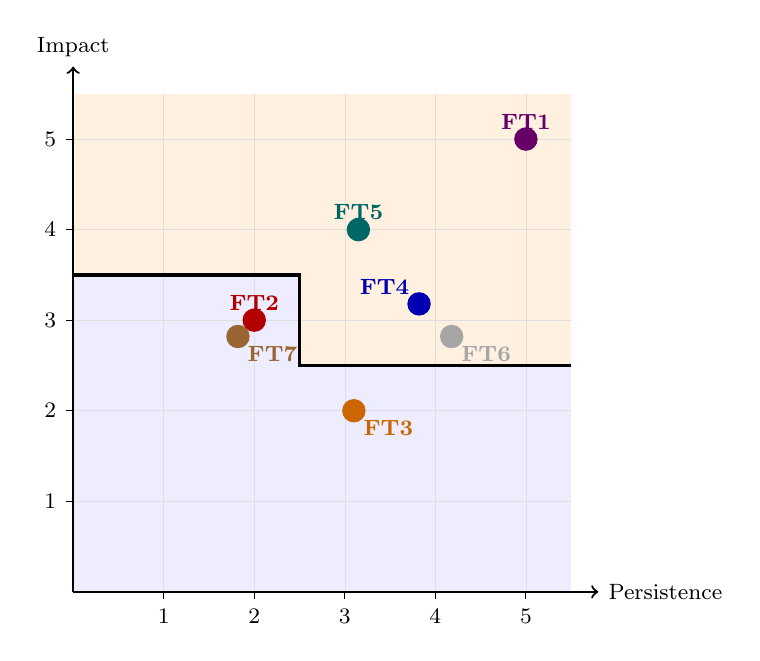
\begin{tikzpicture}[scale=1.15, font=\small]

  % --- Background zones ---
  \fill[orange!12]
    (0,3.5) rectangle (2.5,5.5);
  \fill[orange!12]
    (2.5,2.5) rectangle (5.5,5.5);
  \fill[blue!7]
    (0,0) rectangle (5.5,2.5);
  \fill[blue!7]
    (0,2.5) rectangle (2.5,3.5);

  % --- Grid ---
  \draw[gray!25, very thin, step=1] (0,0) grid (5.5,5.5);

  % --- Urgency curve (stepped polyline) ---
  \draw[very thick, black]
    (0,3.5) -- (2.5,3.5) -- (2.5,2.5) -- (5.5,2.5);

  % --- Axes ---
  \draw[->, thick] (0,0) -- (5.8,0)
    node[right, font=\footnotesize] {Persistence};
  \draw[->, thick] (0,0) -- (0,5.8)
    node[above, font=\footnotesize] {Impact};

  % --- X-axis ticks and labels ---
  \foreach \x in {1,2,3,4,5}{
    \draw (\x, 0) -- (\x,-0.08) node[below, font=\footnotesize] {\x};
  }
  % --- Y-axis ticks and labels ---
  \foreach \y in {1,2,3,4,5}{
    \draw (0,\y) -- (-0.08,\y) node[left, font=\footnotesize] {\y};
  }

  % FT1 --- P=5, I=5
  \filldraw[violet!80!black] (5,5) circle (3.5pt);
  \node[violet!80!black, font=\footnotesize\bfseries, above]
    at (5,5) {FT1};

  % FT2 --- P=2, I=3
  \filldraw[red!70!black] (2,3) circle (3.5pt);
  \node[red!70!black, font=\footnotesize\bfseries, above]
    at (2,3) {FT2};

  % FT3 --- P=3, I=2
  \filldraw[orange!80!black] (3.1,2) circle (3.5pt);
  \node[orange!80!black, font=\footnotesize\bfseries, below right]
    at (3.1,2) {FT3};

  % FT4 --- P=4, I=3 (offset ↖)
  \filldraw[blue!70!black] (3.82,3.18) circle (3.5pt);
  \node[blue!70!black, font=\footnotesize\bfseries, above left]
    at (3.82,3.18) {FT4};

  % FT5 --- P=3, I=4 (offset right)
  \filldraw[teal!80!black] (3.15,4) circle (3.5pt);
  \node[teal!80!black, font=\footnotesize\bfseries, above]
    at (3.15,4) {FT5};

  % FT6 --- P=4, I=3 (offset ↘)
  \filldraw[gray!70] (4.18,2.82) circle (3.5pt);
  \node[gray!70, font=\footnotesize\bfseries, below right]
    at (4.18,2.82) {FT6};

  % FT7 --- P=2, I=3 (offset ↙ from FT2)
  \filldraw[brown!80!black] (1.82,2.82) circle (3.5pt);
  \node[brown!80!black, font=\footnotesize\bfseries, below right]
    at (1.82,2.82) {FT7};

\end{tikzpicture}
\caption{Urgency curve --- issues emerged from the Formative Test. The stepped curve
  separates issues to fix immediately (orange zone, right of the threshold) from those
  to monitor in the next release (blue zone). Issues with equal impact/persistence are
  offset for readability (FT4, FT6).}
\label{fig:urgency-curve-ft}
\end{figure}

\vspace{0.3cm}

\noindent\begin{tabular}{lccc}
\toprule
\textbf{Label} & \textbf{Issue} & \textbf{P} & \textbf{I} \\
\midrule
FT1 & Terminological ambiguity ``Dove Comprare'' vs ``Abbonamenti'' & 5 & 5 \\
FT2 & Absence of ``First access'' onboarding & 2 & 3 \\
FT3 & Channel wizard not personalized by age & 3 & 2 \\
FT4 & Help page without direct links & 4 & 3 \\
FT5 & ``Cannot purchase on tper.it'' message disorienting & 3 & 4 \\
FT6 & Missing ``Print'' button in wizards & 4 & 3 \\
FT7 & Link to timetables in route planning & 2 & 3 \\
\bottomrule
\end{tabular}

\vspace{0.2cm}

\subsection*{Name of Redesigned Version}
\begin{tcolorbox}[base]
Redesign TPER --- v2.0 (Interactive prototype --- Phase D)
\end{tcolorbox}

% ================================================================
% SUMMATIVE TEST CARD
% ================================================================

\newpage

\section{Summative Test Card}
\textit{(This test relates to the final redesigned tool, Phase D --- v2.0)}

\vspace{0.2cm}

\subsection*{Name of tool}
\begin{tcolorbox}[base]
Redesign TPER --- v2.0 (Interactive prototype --- Phase D)
\end{tcolorbox}

\vspace{0.2cm}

\begin{center}
  {\color{primaryColor}\large\bfseries Testing protocol}
  \vspace{0.1cm}
  \color{borderColor}\hrule
\end{center}

\vspace{0.2cm}

\subsection*{Testing session setup}
\begin{tcolorbox}[base]
The testing sessions were conducted \textbf{in person},
at the subject's home. The device used was
the researcher's laptop, with
\textbf{Windows 11} operating system, \textbf{Google Chrome} browser updated
to the latest available version, screen resolution 1920$\times$1080.
The researcher was present in the room and did not interact
with the subject during task execution but limited themselves
to explaining the purpose of the site and the activity, consistent
with the \textit{bottom line data} methodology.
\end{tcolorbox}

\vspace{0.2cm}

\subsection*{Testing method}
\textbf{Discount usability testing} (2--5 people)

\vspace{0.2cm}

\subsection*{List of tasks to test}
\begin{tcolorbox}[base]
\begin{enumerate}[leftmargin=*,itemsep=4pt]
  \item \textbf{Timetable search and consultation:} The user must
  find stops and timetables of a specific line (Line 39:
  Left circular peripheral route).
  \item \textbf{Route planning:} The user must
  use the application's features to
  calculate a route setting origin (Piazza Maggiore) and
  destination (Giardini Margherita).
  \item \textbf{Monthly pass purchase:} The user
  must navigate the redesign's architecture to access
  the purchase of an impersonal monthly pass.
  \item \textbf{Benefits and requirements identification:}
  The user must look for the requirements and necessary documents to
  obtain fare reductions for purchasing an
  annual pass in relation to their condition (ISEE, seniors, etc.)
  \item \textbf{Pass renewal:} The user
  must locate the area dedicated to renewing their travel
  pass.
\end{enumerate}
\end{tcolorbox}

\vspace{0.2cm}

\subsection*{Testing methodology}
\textbf{Bottom line data} --- the subject
performs the tasks alone, without interaction with the researcher.
This mode was chosen to collect clean
quantitative data on completion, time, and errors,
not influenced by verbalization or dialogue with
the facilitator.

\vspace{0.2cm}

\subsection*{Metrics of Tests}
\begin{itemize}[leftmargin=*,itemsep=3pt]
  \item \textbf{Success} --- percentage of tasks
  successfully completed.
  \item \textbf{Time} --- time taken to complete
  each task (in seconds).
  \item \textbf{Errors} --- how many errors and which ones were made.
  \item \textbf{Satisfaction} --- collected at the end of the session
  via the SUS scale (10 items). Target expected $\ge 68/100$
  (good usability) on the final redesign.
\end{itemize}

\vspace{0.2cm}

\subsection*{Recruitment of subjects}
\begin{tcolorbox}[base]

\textbf{Laura Palumbo} --- 70 years, F.\\[0.3cm]
\textit{Technical competence:} Low --- uses the smartphone
only for phone calls and WhatsApp messages.\\[0.2cm]
\textit{Domain competence:} Medium --- uses the city bus
daily in Bologna.\\[0.2cm]
\textit{Similarity to the segment:} High --- profile
fully matching \textit{The elderly commuter}
\hyperref[seg:anziana]{[S1]}.\\[0.2cm]
\textit{Connection to the researcher:} Aunt of the researcher
(Stefano Mercurio).

\vspace{0.2cm}

\textbf{Maria Borriello} --- 79 years, F.\\[0.3cm]
\textit{Technical competence:} Very low --- exclusively passive
use of the smartphone (social networks), no experience
with online purchases or digital services.\\[0.2cm]
\textit{Domain competence:} Low --- uses public transport
occasionally, depends on family members for managing the
travel pass.\\[0.2cm]
\textit{Similarity to the segment:} Very high --- most extreme
case of \textit{The elderly commuter} \hyperref[seg:anziana]{[S1]}:
over 75, very low digital competence.\\[0.2cm]
\textit{Connection to the researcher:} Family connection
through proximity network (Francesco Castaldi).

\end{tcolorbox}

\vspace{0.2cm}

\subsection*{Motivation for choice of subjects}
\begin{tcolorbox}[base]
Both subjects were already involved in the Preliminary
User Testing Phase A on the original TPER site, with the same
5 tasks proposed again here. This allows a \textbf{direct
before/after comparison}:

\begin{itemize}[leftmargin=*]
  \item \textbf{Laura Palumbo} (SUS Phase A 37.5/100, 1/5 tasks
  completed) --- ``moderate'' case of the S1 segment: elderly
  with minimal digital autonomy.
  \item \textbf{Maria Borriello} (SUS Phase A 27.5/100, 0/5 tasks
  completed) --- ``extreme'' case of the S1 segment: over 75
  with only passive device use and no active interaction
  with online services.
\end{itemize}

The combination of the two profiles allows evaluating the effectiveness
of the v2.0 redesign on two levels of digital fragility within
the same age group, quantitatively measuring the
improvement compared to Phase A data.
\end{tcolorbox}

% ================================================================
% SUMMATIVE TEST --- INDIVIDUAL RESULTS
% ================================================================

\newpage
\begin{center}
  {\color{primaryColor}\large\bfseries Test \#1: Laura Palumbo}\\
  \vspace{0.1cm}
  \color{borderColor}\hrule
\end{center}

\vspace{0.5cm}

\subsection*{Name}
\begin{tcolorbox}[base]
Laura Palumbo
\end{tcolorbox}

\subsection*{Date and time of test}
\begin{tcolorbox}[base]
June 28, 2026, 5:00 PM
\end{tcolorbox}

\subsection*{Assistant of test (team member)}
\begin{tcolorbox}[base]
Stefano Mercurio
\end{tcolorbox}

\subsection*{Context of test}
\begin{tcolorbox}[base]
Session conducted at the subject's home, in a
familiar and quiet environment. Total duration: 30 minutes
(5 tasks + SUS questionnaire). No notable events.
\end{tcolorbox}

\subsection*{Quantitative data of tests}
\begin{tcolorbox}[base]
Tests were considered failed when the user gave up.
Times were calculated with a dedicated timer.
\begin{center}
\renewcommand{\arraystretch}{1.4}
\begin{tabular}{clcccc}
\toprule
\textbf{Task} & \textbf{Description} &
\textbf{Outcome} & \textbf{Time (s)} &
\textbf{Errors} & \textbf{Backtrack} \\
\midrule
T1 & Timetable search           & \textbf{S} & 96  & 1 & 0 \\
T2 & Route planning              & \textbf{S} & 115 & 1 & 0 \\
T3 & Pass purchase                & \textbf{F} & 84  & 2 & 3 \\
T4 & Benefits and requirements   & \textbf{S} & 57  & 0 & 0 \\
T5 & Pass renewal                 & \textbf{S} & 163 & 3 & 4 \\
\midrule
\multicolumn{2}{l}{\textbf{Totals / Averages}} &
\textbf{4/5 (80\%)} & \textbf{103.0 s} &
\textbf{1.4} & \textbf{1.4} \\
\bottomrule
\end{tabular}
\end{center}

\vspace{0.3cm}
\small S = Success \quad F = Failure \quad
Errors = wrong clicks or incorrect paths \quad
Backtrack = returns to the previous page
\end{tcolorbox}

\subsection*{SUS score}
\begin{tcolorbox}[base]
\textbf{SUS Score: 72.5/100}\\[0.2cm]
\small Score well above the acceptability threshold
(50/100) and above 68/100, a value indicating \textbf{good
usability} according to the standardized SUS scale. The data marks
an improvement of +35 points compared to the Phase A SUS on the original
site (37.5/100), moving the usage perception from
``unacceptable'' to ``good''.
\end{tcolorbox}

\subsection*{Outcomes and reflections useful for design}
\begin{tcolorbox}[base]
The data record a substantial improvement compared to the Phase A
test on the original site: completion rate from 20\%
(1/5) to 80\% (4/5), average time from 183.8 s to 103.0 s
($-$44\%), average errors from 5.0 to 1.4 ($-$72\%). The SUS went
from 37.5/100 to 72.5/100, exceeding the \textbf{good usability} threshold
(68/100) and moving the usage perception from ``unacceptable'' to
``good'' on the standardized scale.

\medskip

Task T2 (route planning), failed in Phase A with
203 s and 6 errors, was successfully completed in 115 s with
only one error, confirming the effectiveness of the
``Cosa vuoi fare?'' grid and the familiar From--To format.

\medskip

Task T3 is the only failure: the terminological barrier
``Dove Comprare'' vs ``Abbonamenti'' (\textbf{FT1}) has not
yet been completely overcome despite the redirect
banners and contextual wizards. The 3 backtrack and 2 errors
indicate that Laura looked for the purchase on the product
page before finding the correct path.

\medskip

The most significant result is task T4 (benefits):
completed with \textbf{zero errors and zero backtrack} in only
57 seconds --- in Phase A the same task had required 195 s
with 7 errors and 4 backtrack. The 4-question benefits wizard
with the ISEE tooltip worked exactly as designed.
\end{tcolorbox}

% ================================================================
% SUMMATIVE TEST --- TEST #2: MARIA BORRIELLO
% ================================================================

\newpage
\begin{center}
  {\color{primaryColor}\large\bfseries Test \#2: Maria Borriello}\\
  \vspace{0.1cm}
  \color{borderColor}\hrule
\end{center}

\vspace{0.5cm}

\subsection*{Name}
\begin{tcolorbox}[base]
Maria Borriello
\end{tcolorbox}

\subsection*{Date and time of test}
\begin{tcolorbox}[base]
June 30, 2026, 4:30 PM
\end{tcolorbox}

\subsection*{Assistant of test (team member)}
\begin{tcolorbox}[base]
Francesco Castaldi
\end{tcolorbox}

\subsection*{Context of test}
\begin{tcolorbox}[base]
Session conducted at the subject's home, in a
familiar and quiet environment. Total duration: 45 minutes
(5 tasks + SUS questionnaire with assisted reading of items).
The subject showed greater familiarity with the device
compared to the Phase A session, although the initial emotion
when facing the trackpad remained visible. A brief
re-orientation phase (3 minutes) was needed to recall browser use.
\end{tcolorbox}

\subsection*{Quantitative data of tests}
\begin{tcolorbox}[base]
Tests were considered failed when the user gave up.
Times were calculated with a dedicated timer.
\begin{center}
\renewcommand{\arraystretch}{1.4}
\begin{tabular}{clcccc}
\toprule
\textbf{Task} & \textbf{Description} &
\textbf{Outcome} & \textbf{Time (s)} &
\textbf{Errors} & \textbf{Backtrack} \\
\midrule
T1 & Timetable search           & \textbf{S} & 162 & 3 & 2 \\
T2 & Route planning              & \textbf{S} & 188 & 4 & 2 \\
T3 & Pass purchase                & \textbf{F} & 141 & 4 & 6 \\
T4 & Benefits and requirements   & \textbf{S} & 98  & 1 & 1 \\
T5 & Pass renewal                 & \textbf{S} & 235 & 5 & 5 \\
\midrule
\multicolumn{2}{l}{\textbf{Totals / Averages}} &
\textbf{4/5 (80\%)} & \textbf{164.8 s} &
\textbf{3.4} & \textbf{3.2} \\
\bottomrule
\end{tabular}
\end{center}

\vspace{0.3cm}
\small S = Success \quad F = Failure \quad
Errors = wrong clicks or incorrect paths \quad
Backtrack = returns to the previous page
\end{tcolorbox}

\subsection*{SUS score}
\begin{tcolorbox}[base]
\textbf{SUS Score: 71.0/100}\\[0.2cm]
\small Score well above the acceptability threshold
(50/100) and above 68/100, a value indicating \textbf{good
usability} according to the standardized SUS scale. The data marks
an improvement of +43.5 points compared to the Phase A SUS on the original
site (27.5/100), moving the usage perception from
``unacceptable'' to ``good''. The percentage improvement
(+158\%) is the highest recorded across the entire test cycle,
confirming the effectiveness of the redesign precisely for the most
fragile user profile.
\end{tcolorbox}

\subsection*{Outcomes and reflections useful for design}
\begin{tcolorbox}[base]
The data record a radical improvement compared to the Phase A
test on the original site: completion rate from 0\%
(0/5) to 80\% (4/5), average time from 652.0 s to 164.8 s
($-$75\%), average errors from 13.0 to 3.4 ($-$74\%). The SUS went
from 27.5/100 to 71.0/100, exceeding the \textbf{good usability} threshold
(68/100).

\medskip

The most important result is that Maria, who in Phase A had not
managed to complete any task, has now completed 4 out of 5 tasks.
Task T1 (timetable search), failed in Phase A with 698 s and 14
errors, was completed in 162 s with 3 errors, demonstrating
the effectiveness of the ``Cosa vuoi fare?'' grid and the visual
channel cards.

\medskip

Task T4 (benefits) deserves particular attention: in
Phase A it had required 543 s with 10 errors and 13 backtrack,
without success. In the redesign it was completed in 98 s with a single
error. The 4-question benefits wizard, with the ISEE
tooltip and very simple language, worked exactly
as designed for the most fragile users.

\medskip

Task T3 is the only failure, as for Laura: the terminological
barrier ``Dove Comprare'' vs ``Abbonamenti'' (\textbf{FT1})
persists. Maria, in particular, stopped on the
``Abbonamenti'' page of \texttt{tper.it} looking for the
purchase button, without recognizing the redirect banners to
\texttt{solweb.tper.it}. The 6 backtrack and 4 errors indicate
that the banner language needs to be further simplified for
users with minimal competence.

\medskip

The comparison with Laura Palumbo (SUS 72.5) shows that the redesign
reduces the performance gap between the two digital fragility
profiles: Maria went from a gap of 10 SUS points compared
to Laura (27.5 vs 37.5 in Phase A) to only 1.5 points (71.0 vs 72.5)
in the Summative, demonstrating that inclusive design for the extreme
case proportionally benefits most those starting from
more disadvantaged conditions.
\end{tcolorbox}

% ================================================================
% SUMMATIVE TEST --- OVERALL CONCLUSIONS
% ================================================================

\newpage
\begin{center}
  {\color{primaryColor}\large\bfseries Conclusions --- Summative Test}\\
  \vspace{0.1cm}
  \color{borderColor}\hrule
\end{center}

\vspace{0.5cm}

\subsection*{SUS Average and Variance}
\begin{tcolorbox}[base]
\begin{center}
\renewcommand{\arraystretch}{1.3}
\begin{tabular}{lcc}
\toprule
\textbf{Subject} & \textbf{SUS Phase A} & \textbf{SUS v2.0} \\
\midrule
Laura Palumbo  & 37.5/100 & 72.5/100 \\
Maria Borriello & 27.5/100 & 71.0/100 \\
\midrule
\textbf{Average} & \textbf{32.5/100} & \textbf{71.75/100} \\
\textbf{Variance} & 50.0 & 1.13 \\
\bottomrule
\end{tabular}
\end{center}

\medskip

The variance drops drastically from 50.0 (Phase A) to 1.13
(v2.0), indicating that the redesign has equalized the user
experience between the two fragility profiles. Both subjects
exceed the good usability threshold (68/100), with an
average improvement of +39.25 SUS points.

\medskip

The average percentage improvement is +121\%, with a peak
of +158\% for Maria Borriello, confirming that inclusive
design produces proportionally greater benefits for
users with lower digital competence.
\end{tcolorbox}

\subsection*{Overall Conclusions}
\begin{tcolorbox}[base]
The Summative Test on the v2.0 redesign confirms the effectiveness of the
design choices adopted:

\begin{itemize}[leftmargin=*]
  \item \textbf{Completion rate}: from 1/5 (20\%) and 0/5 (0\%)
  in Phase A to 4/5 (80\%) for both subjects --- a result
  that demonstrates the accessibility of the redesign for elderly users
  with different levels of digital fragility.
  \item \textbf{Average time}: average reduction of 59.5\% (from
  652 s to 164.8 s for Maria; from 183.8 s to 103.0 s for Laura).
  \item \textbf{Average errors}: average reduction of 73\% (from 13.0
  to 3.4 for Maria; from 5.0 to 1.4 for Laura).
  \item \textbf{Average SUS}: from 32.5/100 (unacceptable) to
  71.75/100 (good usability), with both subjects above
  the 68/100 threshold.
\end{itemize}

\medskip

The main residual criticality is \textbf{FT1} (terminological
ambiguity ``Dove Comprare'' vs ``Abbonamenti''), which
caused the only failure in both tests. A further
iteration on the language of banners and redirects
could bring completion to 100\%.

\medskip

In conclusion, the TPER v2.0 redesign achieves the design
objective of \textbf{good usability} (SUS $\ge$ 68) for
both profiles of the S1 segment (The elderly commuter),
validating the entire user-centered design process
from Phase A to Phase D.
\end{tcolorbox}

% ================================================================
% PROJECT RECAP
% ================================================================

\newpage
\begin{center}
  {\color{primaryColor}\LARGE\bfseries\sffamily Project Recap}\\[0.3cm]
  \color{borderColor}\hrule
\end{center}

\vspace{0.4cm}

\begin{tcolorbox}[sectionbox]
\small

\noindent\textbf{Phase A --- Research and Analysis}
\begin{itemize}[leftmargin=*]
  \item \textbf{Client:} TPER S.p.A. --- Complex digital ecosystem (6 channels), cognitive, linguistic and terminological barriers for fragile users.
  \item \textbf{Segmentation:} 3 priority combinations --- S1 (elderly commuter), S2 (foreign worker), S3 (citizen at the counter).
  \item \textbf{Assessment:} 10 critical issues on the TPER site (Direct + Reverse Analysis), 10 on competitor ATAC.
  \item \textbf{User Testing:} 4 subjects, average SUS 37.5/100 (unacceptable), 6/20 tasks completed (30\%).
  \item \textbf{Recommendations:} 13 design recommendations (R1--R13) divided into 6 macro-areas.
\end{itemize}

\vspace{0.2cm}

\noindent\textbf{Phase B --- Personas and Cast}
\begin{itemize}[leftmargin=*]
  \item \textbf{Protagonist:} Fatima Benali (68 years, Moroccan, illiterate in written Italian) --- icon of inclusive design.
  \item \textbf{Cast:} 4 personas (Fatima, Liliana, David, Roberto) with C\&A profiles, 5 narrated use cases.
  \item \textbf{Requirements:} 43 functional requirements (RF-01\ldots{}RF-43) + 10 cast requirements (PR-01\ldots{}PR-05, UR-01\ldots{}UR-05).
\end{itemize}

\vspace{0.2cm}

\noindent\textbf{Phase C --- Design}
\begin{itemize}[leftmargin=*]
  \item \textbf{IA:} Mixed top-down/bottom-up approach, label reorganization, 5 metadata fields, 9 navigation aids.
  \item \textbf{Blueprint:} 3 diagrams (IA tree, multi-channel ecosystem, user journey with trainer-mode).
  \item \textbf{Wireframe:} 8 screens (WF1--WF7b) covering the entire tper.it + solweb ecosystem.
  \item \textbf{Comparison:} 5 Before/After comparisons with 16 structural differences.
  \item \textbf{Design Summary:} 10 issues resolved, traceable from Phase A/B requirements to Phase D tests.
\end{itemize}

\vspace{0.2cm}

\noindent\textbf{Phase D --- Validation}
\begin{itemize}[leftmargin=*]
  \item \textbf{Cognitive Walkthrough:} 11 issues (CW-01\ldots{}CW-11) across 5 tasks, 9 recommendations implemented in v2.0.
  \item \textbf{Formative Test:} 2 subjects, average SUS 57.5/100, 90\% completion, urgency curve FT1--FT7.
  \item \textbf{Summative Test:} 2 subjects (same as Phase A), average SUS \textbf{71.75/100} (good usability), completion rate 80\%, error reduction --73\%, variance reduced from 50.0 to 1.13.
\end{itemize}

\vspace{0.2cm}

\begin{center}
\renewcommand{\arraystretch}{1.3}
\begin{tabular}{lcc}
\toprule
\textbf{Key metric} & \textbf{Phase A} & \textbf{Phase D (v2.0)} \\
\midrule
Average SUS & 32.5/100 & \textbf{71.75/100} \\
Tasks completed & 1/10 (10\%) & \textbf{8/10 (80\%)} \\
SUS variance & 50.0 & \textbf{1.13} \\
Average task time & 417.9 s & \textbf{133.9 s} \\
\bottomrule
\end{tabular}
\end{center}

\vspace{0.2cm}
\small Note: Phase A values refer to the subset of the 2 retested subjects (Laura Palumbo and Maria Borriello), not the average of the 4 original subjects.

\vspace{0.2cm}

\noindent The \textbf{Help People Help People} project redesigned the TPER digital experience \textbf{putting the fragile user at the center}: seniors, foreigners, citizens with low digital competence. The quantitative and qualitative results confirm that an inclusive and guided design produces measurable benefits for everyone, and proportionally greater benefits for those starting from more disadvantaged conditions.

\end{tcolorbox}

\end{document}
